% The packages used here are just a sample. You may need others, and may not need some of these. It doesn't hurt to leave them in, unless they start to conflict with other packages you've added. Chapter 2 has example code for equations, figures, tables, citations, abbreviations, etc. If there are sections labeled 'optional' that you don't want, just comment them out. -jg

%\documentclass[reqno,12pt,oneside]{umdiss2-proposal} % right-side equation numbering, 12 point font, print one-sided 
\documentclass[reqno,12pt,oneside]{report} % right-side equation numbering, 12 point font, print two-sided, Chapters start on odd pages. Rackham only accepts one-sided, so this is for personal printings.
%\documentclass[reqno,12pt,twoside,openright]{report} % right-side equation numbering, 12 point font, print two-sided, Chapters start on odd pages. Rackham only accepts one-sided, so this is for personal printings.

\usepackage{rac}         % Use Rackham thesis style file
\usepackage{aas_macros}  % To allow the reading of ADS journal references in the bibliography
\usepackage[intlimits]{amsmath} % Puts the limits of integrals on top and bottom
\usepackage{amsxtra}     % Use various AMS packages
\usepackage{amsthm}
\usepackage{amssymb}
\usepackage{amsfonts}
\usepackage{graphicx}    % Add some packages for figures. Read epslatex.pdf on ctan.tug.org
\usepackage{rotating}
\usepackage{color}
\usepackage{epsfig}
%\usepackage{subfigure}   % To make subfigures. Read subfigure.pdf on ctan.tug.org
\usepackage{subfig}   % To make subfigures. Read subfigure.pdf on ctan.tug.org
\usepackage{verbatim}
%\usepackage{natbib}      % Allows you to use BibTeX
\usepackage[printonlyused]{acronym} % For the List of Abbreviations. Read acronym.pdf on ctan.tug.org
\usepackage{setspace}    % Allows you to specify the line spacing
\usepackage{listings}    % Allows you to write code in a given language 
\usepackage{filecontents}
\usepackage{tabularx}
\usepackage{dcolumn}
\usepackage{hyphenat}
%Change font to Arial
\renewcommand{\sfdefault}{phv} % Arial
\renewcommand{\familydefault}{\sfdefault}
\newcommand{\fixme}[1]{\noindent \textbf{\textcolor{red}{[ Fixme: #1]}}}

\newcolumntype{d}{D{.}{.}{2.1}}
\doublespacing           % \onehalfspacing for 1.5 spacing, \doublespacing for 2.0 spacing.
%\onehalfspacing
\newcommand{\sun}{\ensuremath{\odot}} % sun symbol is \sun
\newcommand{\ignore}[1]{}
\usepackage{pifont}
\newcommand*\mycirc[1]{{\large \ding{\numexpr201+#1\relax}}}
\usepackage{breakurl}

% required to break long URLS sanely
\PassOptionsToPackage{hyphens}{url} \usepackage{hyperref}
\expandafter\def\expandafter\UrlBreaks\expandafter{\UrlBreaks% save the current one 
\do\a\do\b\do\c\do\d\do\e\do\f\do\g\do\h\do\i\do\j% 
\do\k\do\l\do\m\do\n\do\o\do\p\do\q\do\r\do\s\do\t% 
\do\u\do\v\do\w\do\x\do\y\do\z\do\A\do\B\do\C\do\D% 
\do\E\do\F\do\G\do\H\do\I\do\J\do\K\do\L\do\M\do\N% 
\do\O\do\P\do\Q\do\R\do\S\do\T\do\U\do\V\do\W\do\X% 
\do\Y\do\Z\do\*\do\-\do\~\do\'\do\"\do\-}%



%%%%%%%%%%%%%%%%%%%%%%%%%%%%%%%%%%%%%%%%%%%%%%%%%%%%%%%%%%%%%%%%%%%%%%%%%%%%%%%

% Various theorem environments. All of the following have the same numbering
% system as theorem.

\theoremstyle{plain}
\newtheorem{theorem}{Theorem}
\newtheorem{prop}[theorem]{Proposition}
\newtheorem{corollary}[theorem]{Corollary}
\newtheorem{lemma}[theorem]{Lemma}
\newtheorem{question}[theorem]{Question}
\newtheorem{conjecture}[theorem]{Conjecture}
\newtheorem{assumption}[theorem]{Assumption}

\theoremstyle{definition}
\newtheorem{definition}[theorem]{Definition}
\newtheorem{notation}[theorem]{Notation}
\newtheorem{condition}[theorem]{Condition}
\newtheorem{example}[theorem]{Example}
\newtheorem{introduction}[theorem]{Introduction}

\theoremstyle{remark}
\newtheorem{remark}[theorem]{Remark}
%%%%%%%%%%%%%%%%%%%%%%%%%%%%%%%%%%%%%%%%%%%%%%%%%%%%%%%%%%%%%%%%%%%%%%%%%%%%%%%

\numberwithin{theorem}{chapter}     % Numbers theorems "x.y" where x
                                    % is the section number, y is the
                                    % theorem number

%\renewcommand{\thetheorem}{\arabic{chapter}.\arabic{theorem}}

%\makeatletter                      % This sequence of commands will
%\let\c@equation\c@theorem          % incorporate equation numbering
%\makeatother                       % into the theorem numbering scheme

%\renewcommand{\theenumi}{(\roman{enumi})}

%%%%%%%%%%%%%%%%%%%%%%%%%%%%%%%%%%%%%%%%%%%%%%%%%%%%%%%%%%%%%%%%%%%%%%%%%%%%%%

% If printing two-sided, this makes sure that any blank page at the 
% end of a chapter will not have a page number. 
\makeatletter
\def\cleardoublepage{\clearpage\if@twoside \ifodd\c@page\else
\hbox{}
\thispagestyle{empty}
\newpage
\if@twocolumn\hbox{}\newpage\fi\fi\fi}
\makeatother 

%%%%%%%%%%%%%%%%%%%%%%%%%%%%%%%%%%%%%%%%%%%%%%%%%%%%%%%%%%%%%%%%%%%%%%%%%%%%%%

%This command creates a box marked ``To Do'' around text.
%To use type \todo{  insert text here  }.

\newcommand{\todo}[1]{\vspace{5 mm}\par \noindent
\marginpar{\textsc{To Do}}
\framebox{\begin{minipage}[c]{0.95 \textwidth}
\tt\begin{center} #1 \end{center}\end{minipage}}\vspace{5 mm}\par}

%%%%%%%%%%%%%%%%%%%%%%%%%%%%%%%%%%%%%%%%%%%%%%%%%%%%%%%%%%%%%%%%%%%%%%%%%%%%%%%
\begin{document}

\bibliographystyle{ieeetr}    % Set the bibliography style. ieee 
%\bibliographystyle{agu04}    % Set the bibliography style. agu04, plain, alpha, etc.

% Title page as required by Rackham dissertation guidelines
\titlepage{Heterogeneous Memory Management}{Neha Agarwal}{Doctor of Philosophy}
{Computer Science and Engineering}{2017}
{Associate Professor Thomas F. Wenisch, Chair\\
 Professor Ella Atkins, Cognate\\
 Professor Peter M. Chen\\
 Assistant Professor Ronald G. Dreslinski}

% Begin the front matter as required by Rackham dissertation guidelines
\initializefrontsections

% Optional Frontispiece
%\frontispiece{
\includegraphics[width=6in]{figures/cool-picture.png}}

% Optional, but recommended, Copyright page
\copyrightpage{Neha Agarwal}{nehaag@umich.edu}{ORCID iD: 0000-0001-9833-6538}

% Page numbering. If you don't include a frontispiece or copyright page, you'll need to change this for two-sided printing.
\makeatletter
\if@twoside \setcounter{page}{4} \else \setcounter{page}{1} \fi
\makeatother
 
% Optional Dedication page
%\dedicationpage{To--Family\\~\\ Madhu Agarwal (Mummy)\\Bal Krishna Agarwal (Papa)\\
%Shyam Mohan Agarwal (Bhaiya)\\ Khyati Agarwal (Bhabhi)}
\dedicationpage{To--Family}

% Optional Acknowledgements page
\startacknowledgementspage
First and foremost I want to sincerely thank Tom, my PhD advisor, who gave me the
opportunity to pursue the doctoral program with his guidance. Tom is a fantastic
advisor, a statement that I have been saying time and again especially new
students seeking an advisor. In Indian culture we have a special place and
respect for the ``guru'' and I feel that I was fortunate enought to find Tom and
to be able to associate with him as my ``guru''. Tom is a highly energetic,
optimistic, professional, and extremely knowledgeable person. His advising style
is very adaptive and he let's each student learn and work at his/her own pace.
He does not create work pressure, but if you are going off tracks he will for
sure warn you. He is extremely adaptive and flexible advisor be it technically,
administratively, or logistically. Because of his support I was able to explore
different positions in industry and understand the contrasting but complementary
research approaches in academia versus industry. With his guidance I have learnt
to deal with rejections and failures with a positive attitude, which is an
instrumental medicine for PhD journey. No matter how many rejections you get,
his philosophy of keep trying to improve and doing excellent quality research is
what I found most useful as his student. I am thankful to University of
Michigan, CSE department to give me a wonderful opportunity of associating with
Tom, as my advisor.

I also want to take this chance to thank all of my collaborators for their
contributions in making my ideas more concrete and provide me the perspective
that I lacked before. I especially want to mention about the guidance and
support I got from David Nellans. Dave was my internship mentor at NVIDIA.  His
approach of conducting product influential research helped me understand impact
of research on products and business utility for a company.  Dave is also a very
good friend who boosts my moral and motivates me to keep doing good work.
Andr\'es Lagar-Cavilla is another important name in my technical career,
because of whom I got interested in Linux and operating systems. His commitment
to help and support his peers inspires me. His help during my internship at
Google was the stepping stone for my success in my internship project.

I think coming into the PhD program was one of the best decisions of my life. I
got many opportunities to travel in the last six years, exploing different
countires, culutres, and lifestyles. Travel gave me a perspective to meaning of
life. I could go out of my comfort zone, experience people's generosity,
overcome difficulty of not knowing whereabouts of a plcae. I realized that world
is a much bigger and beautiful place and that experience matters more than
success. Travel inspired me to explore new avenues in my research, become
comfortable at switching projects and keep learning new things.

My parents -- Madhu Agarwal and Bal Krishna Agarwal -- are the reason whatever I
am today. Their constant guidance and support in life has been instrumental in
my writing this acknowledgement section today. They have provided me the shade
and comfort at each and every single step in my life even when I didn't ask for
it. They always understand what I need and are always there for me. The feeling
of having them no matter what happened in my professional or personal life is
the biggest gift I have gotten in my life. When things were not going the way I
wanted them to go for very long time and I was doubting myself all the time,
mummy papa were the one who always filled me with confidence and encouraged me
to try even harder. I have called them several times late at nights to talk about
how worried I am, how things are not happening even though I am doing all I can,
they are always there to listen to me quietly and help me move forward. I can't
imagine doing anything without their support. Thanks is a small word for what my
parents have done for me. I can just say that I am lucky enough to have them in
my life. Mummy--Papa this dissertation is your hard work and you confidence in
me to be able to sincerely work and contribute to the world.

Next, I want to talk about my brother, Shyam Mohan Agarwal. He is the person who
loves me so much that at times I think what did I do to receive that much love.
He is the one because of whom I am able to fulfill my dream of studying in
the best institutes of knowledge. His encouragement and belief in me is why I
have the courage to try out new things fearlessly. He looked something in me
since childhood and he knew that I would be a scholar. It has been like he has
foreseen what I will become and then gave me a push to go and get it. With every
achievement of mine it feels like he actually won something. He is the one who
enjoys my success the most. Without him experiencing the joy of what I do my
work is incomplete. He is a true inspiration to me, without whom I am not sure
how I would have a direction to pursue something that I love most doing. I also
want to thank my sister-in-law, Khyati Agarwal, who has been so nice to
accommodate all of us in her life and continued to make our family loving and
happy.

I have also been very fortunate to have come accross several fantastic people and be
friends with them. Gaurav, Pooja, Kataria, Gauri, Tanvi, Mohit, Kunal, Pulkit
are some names very close to my heart that I know will come for me if I need
them at any point in life. They have challenged me in several ways, making me a
better person with every interaction. Countless nights we have just sat together
and just discussed some weired mystery of life or just cribbed about how things
are unfair. These people are treasures I have found in my life and have made my
life so comfortable and loving. They have played a significant role by keeping
me sane during the most self-doubting periods of PhD journey. All of my seniors
Gaurav Chadha, Ankit Sethia, Daya Khudia, and Abhayendra Singh are some of the
people who helped me acclimitize in Ann Arbor and the department during my
foundational years of my PhD.

I want to thank my labmates for being very supportive all throughout my graduate
school. Steve Pelley has been a mentor to me and I always go to him to ask for
all sorts of career advice. Faissal Sleiman is a hard working person who always
inspires me to do the right thing. Akshitha, Vaibhav, Amlan, Aasheesh, Jeff all
have been some of the fantastic, smart, and hard working individuals I have come
across, who are like extended family to me. I also want to acknowledge CSE staff
members Dawn Freysinger, Lauri Johnson, Karen Liska, Denise Duprie, and Stephen
Reger who have helped in every possible way whenever I needed
administrative/logistics support from the department.

Finally, I would like to mention the most significant person Subhasis Das,
because of whom I have been able to survive the graduate school. He is the most
amazing person that has happened to me in this life after having blessed with a
fantastic family. This is the person without whom last five years would have been
extremely hard. Even after living miles away he can bring smile on my face in
seconds and make everything look good again. His presence in my life is
priceless and I can't thank God enough for bringing him in my life.  I will
cherish all the fun we had discussing technical stuff, watching Netflix
together and a getaway from cold Ann Arbor. I have learnt a lot from Subhasis's
technical approach and his philosophy that at times you got to try million
things before something actually starts working or is meaningful. Thanks so much
for being part of my life, without you this journey will be incomplete.


\label{Acknowledgements}

% Optional Preface page
%\startprefacepage
%\input{Preface}
%\label{Preface}

% Table of contents, list of figures, etc.
\tableofcontents     % Required
\listoffigures       % Required if there is more than one figure
\listoftables        % Required if there is more than one table
%\listofmaps          % Required if there is more than one map
%\listofappendices    % Required if there is more than one appendix
%\listofabbreviations % Optional. Abbreviations should be stored in a file named abbr.tex

% Optional in-dissertation Abstract Page
\startabstractpage
{Heterogeneous Memory Management}{Neha Agarwal}{Chair: Thomas F. Wenisch}
Systems from smartphones, data-centers to supercomputers are increasingly
heterogeneous, being composed of different memory technologies. To maximize
performance per dollar, these systems will increasingly use globally-addressable
heterogeneous memory systems, making decisions about memory management critical
to performance. Heterogeneous memory systems pose multi-fold challenges on
system programmability, design and verification. Memory management is a
challenging problem as choices about data placement, movement have to be made at
application runtime desirable in an application-transparent manner, while also
considering different bandwidths, latencies, and costs-per-bit of different
memory technologies. In this thesis we tackle memory management of broadly two
categories of heterogeneous systems: a) CPU-GPU systems with unified virtual
address space, b) Cloud computing platforms that will have deploy cheaper but
slower memory technologies along with DRAMs.
%We discuss the challenges presented by upcoming heterogeneous CPU-GPU memory
%systems and propose solutions to enable their adoption by simplifying the
%programming model and design and verification efforts needed to build such
%complex systems.
We show that current page placement policies are not sufficient to maximize GPU
performance in heterogeneous CPU-GPU memory systems and propose an application
agnostic Bandwidth-Aware (BW-AWARE) placement policy that maximizes GPU
throughput by balancing page placement across the memories based on the
aggregate memory bandwidth available in a system.
%Our results show that BW-AWARE placement outperforms the existing Linux
%INTERLEAVE and LOCAL policies by 35\% and 18\% on average for GPU compute
%workloads.  We build upon BW-AWARE placement by developing a compiler-based
%profiling mechanism that provides programmers with information about GPU
%application data structure access patterns.  Combining this information with
%simple program-annotated hints about memory placement, our hint-based page
%placement approach performs within 90\% of oracular page placement on average,
%largely mitigating the need for costly dynamic page tracking and migration.
%
%Historically, GPU-based HPC applications have had a substantial memory
%bandwidth advantage over CPU-based workloads due to using GDDR rather than DDR
%memory.  However, past GPUs required a restricted programming model where
%application data was allocated up front and explicitly copied into GPU memory
%before launching a GPU kernel by the programmer. Recently, GPUs have eased this
%requirement and now can employ on-demand software page migration between CPU
%and GPU memory to obviate explicit copying.  In the near future, CC-NUMA
%GPU-CPU systems will appear where software page migration is an optional choice
%and hardware cache-coherence can also support the GPU accessing CPU memory
%directly.
To enhance programmability we explore dynamic page migration policies that do
not require any programmer annotation.
%We describe the trade-offs and considerations in relying on hardware
%cache-coherence mechanisms versus using software page migration to optimize the
%performance of memory-intensive GPU workloads.
We show that page migration decisions based on page access frequency
alone are a poor solution and that a broader solution using virtual
address-based program locality to enable aggressive memory prefetching combined
with bandwidth balancing is required to
maximize performance.
%We present a software runtime system requiring minimal hardware support that,
%on average, outperforms CC-NUMA-based accesses by 1.95$\times$, performs 6\%
%better than the legacy CPU to GPU {\tt memcpy} regime by intelligently using
%both CPU and GPU memory bandwidth, and comes within 28\% of oracular page
%placement, all while maintaining the relaxed memory semantics of modern GPUs.
%
To address the design and verification challenges of implementing hardware cache
coherence in heterogeneous CPU-GPU systems 
%Cache coherence is ubiquitous in shared memory multi\hyp{}processors because it
%provides a simple, high performance memory abstraction to programmers.  Recent
%work suggests extending hardware cache coherence between CPUs and GPUs to help
%support programming models with tightly coordinated sharing between CPU and GPU
%threads.  However, implementing hardware cache coherence is particularly
%challenging in systems with discrete CPUs and GPUs that may not be produced by
%a single vendor. Instead,
we propose selective caching, wherein we disallow GPU caching of any memory that
would require coherence updates to propagate between the CPU and GPU, thereby
decoupling the GPU from vendor-specific CPU coherence protocols.
%We propose several architectural improvements to offset the performance penalty
%of selective caching including aggressive request coalescing, CPU-side coherent
%caching for GPU-uncacheable requests, and CPU--GPU interconnect optimizations.
%Moreover, current GPU workloads access many read-only memory pages; we exploit
%this property to allow promiscuous GPU caching of these pages, relying on
%page-level protection, rather than hardware cache coherence, to ensure
%correctness.   These optimizations bring a selective caching GPU implementation
%to within 93\% of a hardware cache-coherent implementation without the need to
%integrate CPUs and GPUs under a single hardware coherence protocol.

The advent of denser/cheaper memory technologies has renewed interest in
two-tiered main memory schemes, where cold data are shifted to slow memory to
enable greater capacity or reduce cost.  Past research on two-tiered main memory
has assumed a 4KB page size.  However, our recent work demonstrates that 2MB
(transparent) huge pages are performance critical in Cloud applications.  We
propose to develop a transparent huge-page-aware two-tiered memory solution,
targeting virtualized cloud applications, which integrates support for dynamic
page migration and transparent huge pages, achieving both the capacity/cost
advantages of two-tiered memory and performance advantages of huge pages. Hot
regions within otherwise cold huge pages present a central challenge to our
objective. We propose translation facades, a 4KB translation that remaps a
portion of a 2MB mapping with an alternate physical address or permissions, to
facilitate remapping hot portions of cold huge pages.

\label{abstract}

\startthechapters 
% The individual files for each of the chapters are put here.
% Save each chapter of your thesis to a seperate tex file
% and then use the \input command to include this file in your
% thesis.  For instance you can save a file to "intro.tex" and 
% then type %{\color{red}
%\begin{itemize}
%\item New memory technologies
%\item Why is virtual address shared space is a challenge with the advent of
%these new technologies
%
%\item How is CPU--GPU space changing in terms
%of high bandwidth but lower latency interconnects
%\item Present opportunities and challenges
%\item Combine intro of first 3 GPU papers
%
%\item Google Proposal
%\item How cheaper but slower mem technologies can lead to boosting perf/dollar
%in data-centers
%\item Present opportunities and challenges
%\end{itemize}
%}
%
The emergence of {\it heterogeneous memory systems} has resulted in a need for
new memory management policies that are able to fully exploit these systems.
While traditional memory management techniques largely assume a ``homogeneous''
main memory, future systems are likely to have two or more different types of
main memories attached to them -- thus the term ``heterogeneous'' memory
systems. An example of such system is the recently announced NVIDIA's Pascal
GPU~\cite{pascal}, which is slated to have high bandwidth connection to the host
CPU by NVLink~\cite{NVLINK} and thus can access host memory seamlessly.  Another
example is Intel's 3-D XPoint technology~\cite{xpoint}, which provides a slow
but cheaper and large capacity non-volatile memory (NVRAM) along with a regular
DRAM based memory attached to the same CPU node.  There are several aspects of
such systems that have not been studied before:

\begin{enumerate}
\item
\textbf{Different bandwidths:}
Different memory technologies will typically have differences in their
bandwidths, e.g., a GPU connected to on-board GDDR and host-side DDR memories
can have a bandwidth differential of $\approx$ 2 -- 8 $\times$ between the two
memory technologies. Since GPUs are sensitive to main memory bandwidth, the
metric to optimize for in such systems is the total available bandwidth to the
GPU from the two memory sources. While prior work on Non-Uniform Memory Access
(NUMA) has closely looked at data placement strategies to optimize the total
memory {\it access latency} in the presence of different memory zones with
different access latencies, we show that such policies are not suited to
optimizing the total memory {\it bandwidth}. Instead, we propose {\it
Bandwidth-Aware Placement} (BW-AWARE), which directly maximizes the overall
bandwidth, and show that it can significantly increase application throughput
for several GPU applications.

\item
\textbf{Different coherency domains:} 
In a heterogeneous CPU-GPU memory system, implementing hardware cache coherence
between the CPU and the GPU can lead to a significant challenges because of
design and verification involved particularly if the two domains are designed by
separate vendors. We introduce {\it Selective Caching}, a coherence policy that
disallows GPU caching of any memory that would require coherence updates to
propagate across the two domains. This approach decouples the cache-coherence
protocols in CPUs and GPUs, thus improving cross-vendor design cycle time.

\item
\textbf{Different costs per bit:}
Different memory technologies can have different costs.  For example, recently
announced non-volatile memory technology~\cite{xpoint} is projected to be
significantly cheaper than regular DRAM, while also being significantly higher
latency. Their lower cost per bit makes them a good candidate for use in
data-centers, where main memory cost can be up to $\approx$ 30\% of the total
cost of ownership (TCO). However, their low speed means that only {\it cold},
i.e., infrequently accessed data can be placed in such memories. However, placing more
cold data in the slower memories conflicts with efficient virtual memory usage
by transparent huge page (THP), which can provide 10-15\% performance gains in
large memory footprint data-center applications. We study how to reap the
benefits of huge pages while also placing as much data in slow memory as
possible, to improve performance per dollar in data-centers.
\end{enumerate}

Below, we describe each of these three problems in detail and give a brief
sketch of our proposed solution to these problems.

\section{Bandwidth-asymmetric Systems}
To date, GPU-attached Bandwidth-Optimized (BO) memory has been allocated and
managed primarily as through explicit, programmer-directed function calls.
To make best use of the bandwidth available to GPU programs, programmers
manually copy the data over the relatively slow PCIe bus to the GPU memory, and
--- only then --- launch their GPU kernels.  This up-front data allocation and
transfer has been necessary since transferring data over the PCIe bus is a high
overhead operation, and a bulk transfer of data amortizes this overhead. This
data manipulation overhead also results in significant porting challenges when
retargeting existing applications to GPUs, particularly for high-level languages
that make use of libraries and dynamic memory allocation during application
execution.

\begin{figure}[t]
    \centering
    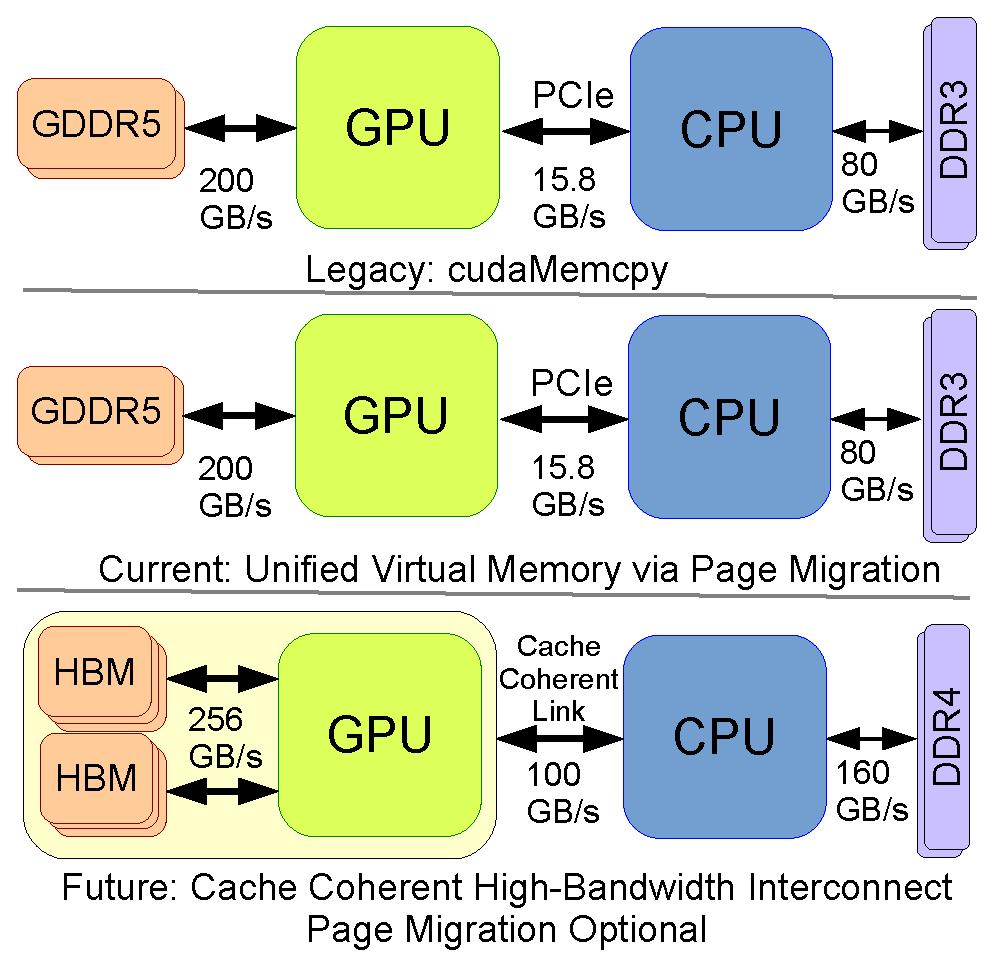
\includegraphics[width=0.7\columnwidth]{hpca2015/figures/architecture.eps}
    \caption{System architectures for legacy, current, and future mixed GPU-CPU systems.}
    \label{fig:arch-hpca2015}
\end{figure}

Recognizing the obstacle this programming model poses to the wider adoption of
GPUs in more parallel applications, programming systems like NVIDIA's CUDA,
OpenCL, and OpenACC are evolving to shared virtual address space between CPU and
GPU~\cite{UVM}. Concurrently, CPU-GPU architectures are evolving to have unified
globally addressable memory systems in which both the GPU and CPU can access any
portion of memory at any time, regardless of its physical location.  Today this
unified view of memory is layered on top of legacy hardware designs by
implementing software-based runtimes that dynamically copy data on demand
between the GPU and CPU~\cite{cuda}. As depicted in
Figure~\ref{fig:arch-hpca2015}, over the next several years it is expected that
GPU and CPU systems will move away from the PCIe interface to a fully cache
coherent (CC) interface ~\cite{AMDHSA}. These systems will provide high
bandwidth ($5-10x$ higher) and low latency ($10x$ lower) between the non-uniform memory
access (NUMA) pools attached to discrete processors by layering coherence
protocols on top of physical link technologies such as NVLink~\cite{NVLINK},
Hypertransport~\cite{AMDHT}, or QPI~\cite{INTELQPI}.   CC-NUMA access to
CPU-attached memory from the GPU makes the software page migration used today an
optional feature thanks to the improved bandwidth, latency, and access
granularity that cache coherence can provides.

As heterogeneous CPU-GPU systems move to a transparent unified memory system,
the OS and runtime systems need information about other aspects of memory zones
such as their bandwidths instead of only the access latency information that is
exposed today via Advanced Configuration and Power Interface (ACPI). In CC-NUMA
systems today, latency information alone is adequate as CPUs are generally more
performance sensitive to memory system latency rather than other memory
characteristics. In contrast, massively parallel GPUs and their highly-threaded
programming models have been designed to gracefully handle long memory
latencies, instead demanding high bandwidth. Unfortunately, differences in
bandwidth capabilities, read versus write performance, and access energy are not
exposed to software; making it difficult for the operating system, runtime, or
programmer to make good decisions about memory placement in these GPU-equipped
systems. In this thesis we investigate the effect on GPU performance of exposing
memory system bandwidth information to the operating system/runtime and user
applications to improve the quality of dynamic page placement and migration
decisions.

\section{Different Coherence Domains}
%Technology trends indicate an increasing number of systems designed with CPUs,
%accelerators, and GPUs coupled via high-speed links. Such systems are likely to
%introduce unified shared CPU-GPU memory with shared page tables. In fact, some
%systems already feature such implementations~\cite{AMDKaveri}.
Introducing globally visible shared memory improves programmer productivity by
eliminating explicit copies and memory management overheads. Whereas this
abstraction can be supported using only software page-level protection
mechanisms~\cite{UVM, HSA}, hardware cache coherence can improve performance by
allowing concurrent, fine-grained access to memory by both CPU and GPU.
%If the CPU and GPU have separate physical memories, page migration may also be
%used to optimize page placement for latency or bandwidth by using both near and
%far memory~\cite{Dashti2013,Agarwal2015b,Meswani2015,Chou2015}.

%Some CPU--GPU systems will be tightly integrated into a system on chip (SoC)
%making on-chip hardware coherence a natural fit, possibly even by sharing a
%portion of the on-chip cache hierarchy~\cite{HSA,AMDAPU,Hechtman2014}.  However,
%the largest GPU implementations consume nearly 8B transistors and have their own
%specialized memory systems~\cite{NVIDIA8BILLION}.  Power and thermal constraints
%preclude single-die integration of such designs.  Thus, many CPU--GPU systems
%are likely to have discrete CPUs and GPUs connected via dedicated off-chip
%interconnects like NVLINK (NVIDIA), CAPI (IBM), HT (AMD), and QPI (INTEL) or
%implemented as multi-chip modules~\cite{NVLINK,CAPI,AMDHT,INTELQPI,Chen92}.
%The availability of these high speed off-chip interconnects has led both
%academic groups and vendors like NVIDIA to investigate how future GPUs may
%integrate into existing OS controlled unified shared memory regimes used by
%CPUs~\cite{Pichai2014,Power2014,Agarwal2015,Agarwal2015b}.

Despite the programmability benefits of CPU-GPU cache coherence, designing such
a system can involve several hurdles. Prior studies~\cite{Hong2012} have shown
that coherence implementations are a major source of hardware design bugs.
Extending a CPU coherence implementation to a GPU over a long-latency
interconnect ($approx$ 100ns)  will only increase the design cost of such a system.
Also, if the CPUs and GPUs are to be manufactured by different vendors, a high
level of coordination has to be done between those two vendors -- including
coordination on the specification of coherence implementation and verification
efforts. Such hurdles make CPU-GPU cache coherence an unattractive option to
deploy in a product.

Current CPUs have up to 18 cores per socket~\cite{INTELXEONE5V3} but GPUs are
expected to have hundreds of streaming multiprocessors (SMs) each with its own
cache(s) within the next few years. Hence, extending traditional hardware
cache-coherency into a multi-chip CPU-GPU memory system requires coherence
messages to be exchanged not just within the GPU but over the CPU-GPU
interconnect. Keeping these hundreds of caches coherent with a traditional HW
coherence protocol, as shown in Figure~\ref{fig:motivation}, potentially
requires large state and interconnect bandwidth~\cite{Kelm2010,johnson2011}.
Some recent proposals call for data-race-free GPU programming models, which
allow relaxed or scoped memory consistency to reduce the frequency or hide the
latency of enforcing coherence~\cite{Hechtman2014}.  However, irrespective of
memory ordering requirements, such approaches still rely on hardware
cache-coherence mechanisms to  avoid the need for software to explicitly track
and flush modified cache lines to an appropriate scope at each synchronization
point. Techniques like region coherence~\cite{Power2013} seek to scale coherence
protocols for heterogeneous systems, but require pervasive changes throughout
the CPU and GPU memory systems.
%Such approaches also incur highly coordinated design and verification effort by
%both CPU and GPU vendors~\cite{Hong2012} that is challenging when multiple
%vendors wish to integrate existing CPU and GPU designs in a timely manner.

Due to the significant challenges associated with building such cache-coherent
systems, in this thesis, we architect a GPU \textit{selective caching}
mechanism.  This mechanism provides the conceptual simplicity of CPU-GPU
hardware cache coherence and maintains a high level of GPU performance (93\% of
hardware cache-coherent system), but does not actually implement hardware cache
coherence between the CPU and GPU.
%In our proposed selective caching GPU, the GPU does not cache data that resides
%in CPU physical memory, nor does it cache data that resides in the GPU memory
%that is actively in-use by the CPU on-chip caches.
%This approach is orthogonal to the memory consistency model and leverages the
%latency tolerant nature of GPU architectures combined with upcoming low-latency
%and high-bandwidth interconnects to enable the benefits of shared memory.

\section{Proposal: Cheaper Memory Technologies}
Upcoming memory technologies, such as Intel's recently-announced XPoint-3D
memory~\cite{xpoint}, are projected to be $10x$ denser and $2x$ cheaper per
bit than DRAM while providing the byte-addressable load-store interface of
conventional main memory.  Improved capacity and cost per bit comes at the price
of higher access latency, projected to fall somewhere in the range of 500ns to
several microseconds.  The impending commercial availability of such devices has
renewed interest in two-tiered physical memory, wherein part of a system's
physical address space is implemented with the slower, cheaper memory
technology.  Slow memory can result in a net TCO win if the cost savings of
replaced DRAM outweigh cost increase due to reduced program performance or by
enabling a higher peak memory capacity per server than is economically viable
with DRAM alone.  

%Our preliminary results indicate that over half of the memory footprint of
%representative cloud applications (e.g., Cassandra) are identified as cold by
%Linux’s kstaled mechanism, indicating that the corresponding pages have an
%inter-access interval exceeding 120s.  Analytic modeling suggests these pages
%could be shifted to a memory with a 3us access time with negligible (<3\%)
%performance degradation.

%%It's an interesting problem
%Prior academic work has considered two approaches to two-tiered memory: via a
%paging mechanism~\cite{1,2}, wherein accesses to slow memory invoke a page fault that
%must transfer data to fast memory before an access may proceed, and via a
%migration mechanism (as in cache coherent NUMA multiprocessors)~\cite{XXX}, wherein no
%software fault is required.  In the latter scenario, a migration mechanism seeks
%to shuffle pages between tiers to maximize fast-memory accesses.  

%It's an unsolved problem
Prior academic work on two-tiered memory has assumed migration/paging at 4KB
page granularity.  Huge pages, implemented via Linux's Transparent Huge Page
(THP) mechanism, are now ubiquitous and critical for data-center applications,
boosting application performance by 10-15\%.
%Recent work~\cite{JeffPaper} has demonstrated that 2MB huge pages are particularly
%performance-critical under virtualization.  
%For example, our study demonstrates a 20\% throughput improvement for Hadoop and
%a 40\% speedup on random memory probes when using huge pages under
%virtualization.  
However, huge pages thwart prior two-tiered memory proposals for two reasons:
(1) it is too expensive to frequently migrate pages at 2MB granularity, and (2)
hot regions occur within otherwise cold 2MB huge pages can hurt performance if
placed in the slower memory. 

%Here is my idea
We propose to develop a transparent huge-page-aware two-tiered memory solution
that integrates support for dynamic page migration and transparent huge pages,
achieving both the capacity/cost advantages of two-tiered memory and performance
advantages of huge pages.  Our focus is on cloud computing scenarios where a
high-memory-footprint application, such as Cassandra, Aerospike, or MySQL, runs
under virtualization and may co-run with other, competing applications.  Hot
regions within otherwise cold huge pages present a central challenge to our
objective; existing x86-Linux provides no mechanism to carve out a 4KB hot
region within a 2MB cold page.

%So, we propose translation facades, a 4KB
%translation that remaps a portion of a 2MB mapping with an alternate physical
%address or permissions.  Current x86-Linux requires non-overlapping mappings due
%to hard-coded page table structure and because TLB entries are replaced
%independently, hence, an uncached 4KB facade to a cached 2MB translation could
%lead to a mis-translation. We will pursue implementations of translation
%facades along two paths. (1) Hardware support: we will extend x86 page table and
%TLB design to support facades. (2) Virtualization: Our existing study of huge
%pages under virtualization demonstrate that a majority of the benefit can be
%obtained if host pages are 2MB even if guest pages are 4KB.  We will investigate
%if the two-level translation from guest to host to machine addresses can be
%exploited to emulate hardware support for translation facades.

%Bulleted list of contributions
We propose to develop a Linux prototype that will to estimate the properties of
a system with the following properties:

\begin{enumerate}
\item
We will measure hot and cold memory fractions at 4KB granularity and within 2MB
huge pages to measure two-tiered memory opportunity. We will use kstaled (an
optional extension to the Linux kernel that tracks pages that have not been
accessed over a fixed time interval) and BadgerTrap~\cite{badgertrap} (a tool to
intercept TLB misses in software) to facilitate this characterization. 

\item
We will develop methods to track hot and cold memory regions at run-time.  A
key challenge lies in efficiently tracking hot regions within an otherwise-cold
huge page, as kstaled provides visibility only at page granularity.  We propose
to investigate sampling methods, e.g., by probabilistically demoting huge pages
or leveraging performance counter infrastructure. 

\item
We will develop an online migration mechanism that can shift data between
fast and slow memory tiers while the application is concurrently executing.  We
draw experience from existing NUMA migration and THP memory defragmentation. We
will implement the migration mechanism in the Linux kernel.

\item
We will develop translation facades, a mechanism that remaps a
portion of a 2MB mapping with an alternate physical address or permissions
(using BadgerTrap to emulate performance) and investigate novel page table and
TLB organizations to support facades.
\end{enumerate}

\section{Contributions}
In this thesis we make following contributions:

\begin{itemize}
\item
We show that existing CPU-oriented page placement policies are not only 
sub-optimal for placement in GPU-based systems, but simply do not have the 
appropriate information available to make informed decisions when optimizing for 
bandwidth-asymmetric memory systems. Exposing additional bandwidth information 
to the OS, as is done for latency today, will be required for optimized decision 
making.

\item
We show that placing all pages in the bandwidth optimized memory is not the best
performing page placement policy for GPU workloads.  We propose a new
bandwidth-aware (BW-AWARE) page placement policy that can outperform Linux's
current bandwidth-optimized INTERLEAVE placement by 35\% and the default latency
optimized LOCAL allocation policy by as much as 18\%, when the application
footprint fits within bandwidth-optimized memory capacity.  

%\item
%For \emph{memory capacity constrained} systems (i.e. bandwidth-optimized memory
%capacity is insufficient for the workload footprint), we demonstrate that using
%simple application annotations to inform the OS/runtime of hot versus cold data
%structures can outperform the current Linux INTERLEAVE and LOCAL page placement
%policies.  Our annotation based policy combined with bandwidth information can
%outperform these page placement policies by 19\% and 12\% respectively, and get
%within 90\% of oracle page placement performance.

\item
We show that counter-based metrics to determine when to migrate pages from the
CPU to GPU are insufficient for finding an optimal migration policy to exploit
GPU memory bandwidth.  In streaming workloads, where each page may be accessed
only a few times, waiting for $N$ accesses to occur before migrating a page will
actually limit the number of accesses that occur after migration, reducing the
efficacy of the page migration operation.

\item
TLB shootdown and refill overhead can significantly degrade the performance of
any page migration policy for GPUs\@. We show that combining reactive migration
with virtual address locality information to aggressively prefetch pages can
mitigate much of this overhead, resulting in increased GPU throughput (35\%).

%\item
%The legacy intuition to migrate all data to the GPU local memory in an attempt
%to maximize bandwidth fails to leverage the bandwidth available via the new
%CC-NUMA interface.  A page migration policy which is aware of this differential
%and balances migration with CC-NUMA link utilization will outperform either GPU
%or GPU memory being used in isolation.

\item 
We present a software based memory migration system that, on average,
outperforms CC-NUMA based accesses by 1.95$\times$, performs 6\% better than the
legacy CPU to GPU {\tt memcpy} approach by intelligently using both CPU and GPU
memory bandwidth, and comes within 28\% of oracular page placement, all while
maintaining the relaxed memory semantics of modern GPUs.

%\vspace{-.025in}
\item
We propose GPU selective caching, which can provide a CPU--GPU system that
provides a unified shared memory without requiring hardware cache-coherence
protocols within the GPU or between CPU and GPU caches.

\item
We identify that much of the improvement from GPU caches is due to coalescing 
memory accesses that are spatially contiguous within a cache line.  Leveraging
aggressive request coalescing, GPUs can achieve much of the performance benefit
of caching (80\%), without caches.

%\item
%We propose a small on-die CPU cache specifically to handle uncached requests
%that will be issued at sub-cache line granularity from the GPU. This cache helps both 
%shield the CPU memory system from the bandwidth hungry GPU and supports
%improved CPU--GPU interconnect efficiency by implementing variable-sized transfer granularity.

\item
We demonstrate that a large fraction (60\%) of GPU-accessed data is read-only.
Allowing the GPU to cache this data and relying on page protection mechanisms
rather than hardware coherence to ensure correctness closes the performance gap
between a selective caching and hardware cache-coherent GPU for many
applications.
\end{itemize}
. 

 \chapter{Introduction}
 \label{chap:intro}
 %{\color{red}
%\begin{itemize}
%\item New memory technologies
%\item Why is virtual address shared space is a challenge with the advent of
%these new technologies
%
%\item How is CPU--GPU space changing in terms
%of high bandwidth but lower latency interconnects
%\item Present opportunities and challenges
%\item Combine intro of first 3 GPU papers
%
%\item Google Proposal
%\item How cheaper but slower mem technologies can lead to boosting perf/dollar
%in data-centers
%\item Present opportunities and challenges
%\end{itemize}
%}
%
The emergence of {\it heterogeneous memory systems} has resulted in a need for
new memory management policies that are able to fully exploit these systems.
While traditional memory management techniques largely assume a ``homogeneous''
main memory, future systems are likely to have two or more different types of
main memories attached to them -- thus the term ``heterogeneous'' memory
systems. An example of such system is the recently announced NVIDIA's Pascal
GPU~\cite{pascal}, which is slated to have high bandwidth connection to the host
CPU by NVLink~\cite{NVLINK} and thus can access host memory seamlessly.  Another
example is Intel's 3-D XPoint technology~\cite{xpoint}, which provides a slow
but cheaper and large capacity non-volatile memory (NVRAM) along with a regular
DRAM based memory attached to the same CPU node.  There are several aspects of
such systems that have not been studied before:

\begin{enumerate}
\item
\textbf{Different bandwidths:}
Different memory technologies will typically have differences in their
bandwidths, e.g., a GPU connected to on-board GDDR and host-side DDR memories
can have a bandwidth differential of $\approx$ 2 -- 8 $\times$ between the two
memory technologies. Since GPUs are sensitive to main memory bandwidth, the
metric to optimize for in such systems is the total available bandwidth to the
GPU from the two memory sources. While prior work on Non-Uniform Memory Access
(NUMA) has closely looked at data placement strategies to optimize the total
memory {\it access latency} in the presence of different memory zones with
different access latencies, we show that such policies are not suited to
optimizing the total memory {\it bandwidth}. Instead, we propose {\it
Bandwidth-Aware Placement} (BW-AWARE), which directly maximizes the overall
bandwidth, and show that it can significantly increase application throughput
for several GPU applications.

\item
\textbf{Different coherency domains:} 
In a heterogeneous CPU-GPU memory system, implementing hardware cache coherence
between the CPU and the GPU can lead to a significant challenges because of
design and verification involved particularly if the two domains are designed by
separate vendors. We introduce {\it Selective Caching}, a coherence policy that
disallows GPU caching of any memory that would require coherence updates to
propagate across the two domains. This approach decouples the cache-coherence
protocols in CPUs and GPUs, thus improving cross-vendor design cycle time.

\item
\textbf{Different costs per bit:}
Different memory technologies can have different costs.  For example, recently
announced non-volatile memory technology~\cite{xpoint} is projected to be
significantly cheaper than regular DRAM, while also being significantly higher
latency. Their lower cost per bit makes them a good candidate for use in
data-centers, where main memory cost can be up to $\approx$ 30\% of the total
cost of ownership (TCO). However, their low speed means that only {\it cold},
i.e., infrequently accessed data can be placed in such memories. However, placing more
cold data in the slower memories conflicts with efficient virtual memory usage
by transparent huge page (THP), which can provide 10-15\% performance gains in
large memory footprint data-center applications. We study how to reap the
benefits of huge pages while also placing as much data in slow memory as
possible, to improve performance per dollar in data-centers.
\end{enumerate}

Below, we describe each of these three problems in detail and give a brief
sketch of our proposed solution to these problems.

\section{Bandwidth-asymmetric Systems}
To date, GPU-attached Bandwidth-Optimized (BO) memory has been allocated and
managed primarily as through explicit, programmer-directed function calls.
To make best use of the bandwidth available to GPU programs, programmers
manually copy the data over the relatively slow PCIe bus to the GPU memory, and
--- only then --- launch their GPU kernels.  This up-front data allocation and
transfer has been necessary since transferring data over the PCIe bus is a high
overhead operation, and a bulk transfer of data amortizes this overhead. This
data manipulation overhead also results in significant porting challenges when
retargeting existing applications to GPUs, particularly for high-level languages
that make use of libraries and dynamic memory allocation during application
execution.

\begin{figure}[t]
    \centering
    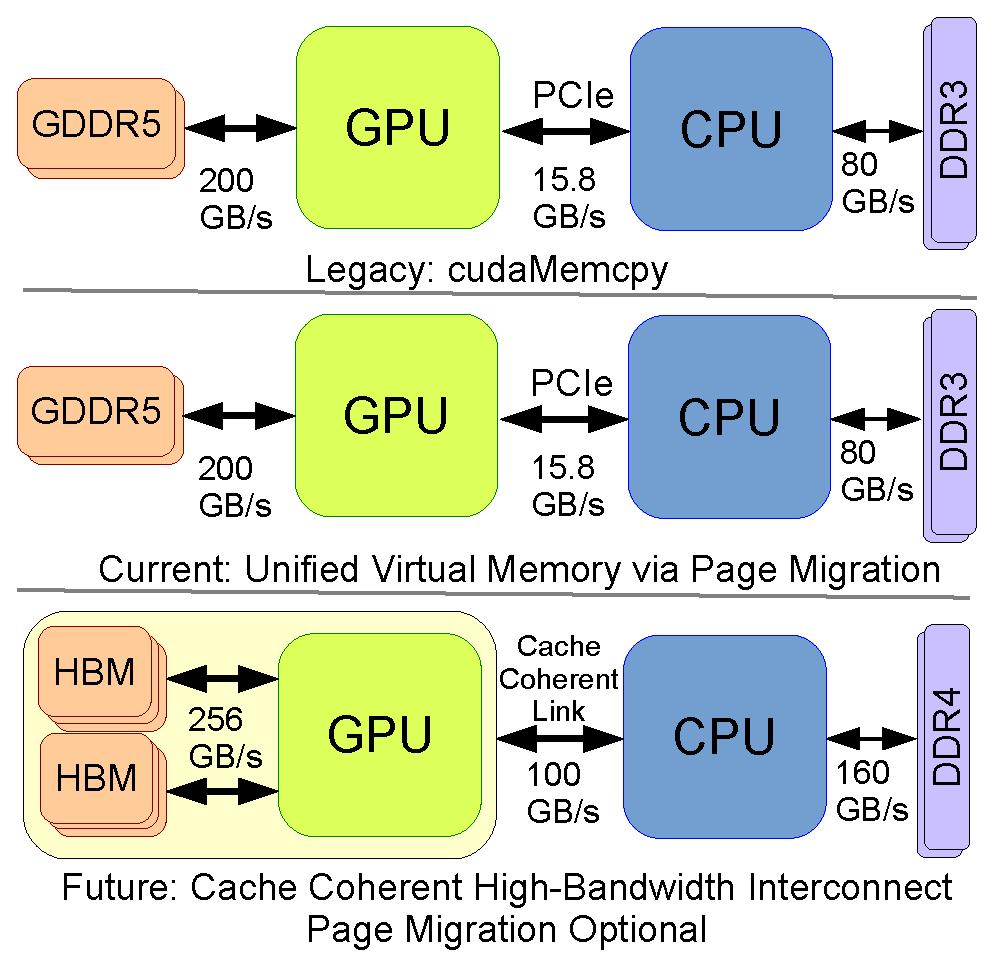
\includegraphics[width=0.7\columnwidth]{hpca2015/figures/architecture.eps}
    \caption{System architectures for legacy, current, and future mixed GPU-CPU systems.}
    \label{fig:arch-hpca2015}
\end{figure}

Recognizing the obstacle this programming model poses to the wider adoption of
GPUs in more parallel applications, programming systems like NVIDIA's CUDA,
OpenCL, and OpenACC are evolving to shared virtual address space between CPU and
GPU~\cite{UVM}. Concurrently, CPU-GPU architectures are evolving to have unified
globally addressable memory systems in which both the GPU and CPU can access any
portion of memory at any time, regardless of its physical location.  Today this
unified view of memory is layered on top of legacy hardware designs by
implementing software-based runtimes that dynamically copy data on demand
between the GPU and CPU~\cite{cuda}. As depicted in
Figure~\ref{fig:arch-hpca2015}, over the next several years it is expected that
GPU and CPU systems will move away from the PCIe interface to a fully cache
coherent (CC) interface ~\cite{AMDHSA}. These systems will provide high
bandwidth ($5-10x$ higher) and low latency ($10x$ lower) between the non-uniform memory
access (NUMA) pools attached to discrete processors by layering coherence
protocols on top of physical link technologies such as NVLink~\cite{NVLINK},
Hypertransport~\cite{AMDHT}, or QPI~\cite{INTELQPI}.   CC-NUMA access to
CPU-attached memory from the GPU makes the software page migration used today an
optional feature thanks to the improved bandwidth, latency, and access
granularity that cache coherence can provides.

As heterogeneous CPU-GPU systems move to a transparent unified memory system,
the OS and runtime systems need information about other aspects of memory zones
such as their bandwidths instead of only the access latency information that is
exposed today via Advanced Configuration and Power Interface (ACPI). In CC-NUMA
systems today, latency information alone is adequate as CPUs are generally more
performance sensitive to memory system latency rather than other memory
characteristics. In contrast, massively parallel GPUs and their highly-threaded
programming models have been designed to gracefully handle long memory
latencies, instead demanding high bandwidth. Unfortunately, differences in
bandwidth capabilities, read versus write performance, and access energy are not
exposed to software; making it difficult for the operating system, runtime, or
programmer to make good decisions about memory placement in these GPU-equipped
systems. In this thesis we investigate the effect on GPU performance of exposing
memory system bandwidth information to the operating system/runtime and user
applications to improve the quality of dynamic page placement and migration
decisions.

\section{Different Coherence Domains}
%Technology trends indicate an increasing number of systems designed with CPUs,
%accelerators, and GPUs coupled via high-speed links. Such systems are likely to
%introduce unified shared CPU-GPU memory with shared page tables. In fact, some
%systems already feature such implementations~\cite{AMDKaveri}.
Introducing globally visible shared memory improves programmer productivity by
eliminating explicit copies and memory management overheads. Whereas this
abstraction can be supported using only software page-level protection
mechanisms~\cite{UVM, HSA}, hardware cache coherence can improve performance by
allowing concurrent, fine-grained access to memory by both CPU and GPU.
%If the CPU and GPU have separate physical memories, page migration may also be
%used to optimize page placement for latency or bandwidth by using both near and
%far memory~\cite{Dashti2013,Agarwal2015b,Meswani2015,Chou2015}.

%Some CPU--GPU systems will be tightly integrated into a system on chip (SoC)
%making on-chip hardware coherence a natural fit, possibly even by sharing a
%portion of the on-chip cache hierarchy~\cite{HSA,AMDAPU,Hechtman2014}.  However,
%the largest GPU implementations consume nearly 8B transistors and have their own
%specialized memory systems~\cite{NVIDIA8BILLION}.  Power and thermal constraints
%preclude single-die integration of such designs.  Thus, many CPU--GPU systems
%are likely to have discrete CPUs and GPUs connected via dedicated off-chip
%interconnects like NVLINK (NVIDIA), CAPI (IBM), HT (AMD), and QPI (INTEL) or
%implemented as multi-chip modules~\cite{NVLINK,CAPI,AMDHT,INTELQPI,Chen92}.
%The availability of these high speed off-chip interconnects has led both
%academic groups and vendors like NVIDIA to investigate how future GPUs may
%integrate into existing OS controlled unified shared memory regimes used by
%CPUs~\cite{Pichai2014,Power2014,Agarwal2015,Agarwal2015b}.

Despite the programmability benefits of CPU-GPU cache coherence, designing such
a system can involve several hurdles. Prior studies~\cite{Hong2012} have shown
that coherence implementations are a major source of hardware design bugs.
Extending a CPU coherence implementation to a GPU over a long-latency
interconnect ($approx$ 100ns)  will only increase the design cost of such a system.
Also, if the CPUs and GPUs are to be manufactured by different vendors, a high
level of coordination has to be done between those two vendors -- including
coordination on the specification of coherence implementation and verification
efforts. Such hurdles make CPU-GPU cache coherence an unattractive option to
deploy in a product.

Current CPUs have up to 18 cores per socket~\cite{INTELXEONE5V3} but GPUs are
expected to have hundreds of streaming multiprocessors (SMs) each with its own
cache(s) within the next few years. Hence, extending traditional hardware
cache-coherency into a multi-chip CPU-GPU memory system requires coherence
messages to be exchanged not just within the GPU but over the CPU-GPU
interconnect. Keeping these hundreds of caches coherent with a traditional HW
coherence protocol, as shown in Figure~\ref{fig:motivation}, potentially
requires large state and interconnect bandwidth~\cite{Kelm2010,johnson2011}.
Some recent proposals call for data-race-free GPU programming models, which
allow relaxed or scoped memory consistency to reduce the frequency or hide the
latency of enforcing coherence~\cite{Hechtman2014}.  However, irrespective of
memory ordering requirements, such approaches still rely on hardware
cache-coherence mechanisms to  avoid the need for software to explicitly track
and flush modified cache lines to an appropriate scope at each synchronization
point. Techniques like region coherence~\cite{Power2013} seek to scale coherence
protocols for heterogeneous systems, but require pervasive changes throughout
the CPU and GPU memory systems.
%Such approaches also incur highly coordinated design and verification effort by
%both CPU and GPU vendors~\cite{Hong2012} that is challenging when multiple
%vendors wish to integrate existing CPU and GPU designs in a timely manner.

Due to the significant challenges associated with building such cache-coherent
systems, in this thesis, we architect a GPU \textit{selective caching}
mechanism.  This mechanism provides the conceptual simplicity of CPU-GPU
hardware cache coherence and maintains a high level of GPU performance (93\% of
hardware cache-coherent system), but does not actually implement hardware cache
coherence between the CPU and GPU.
%In our proposed selective caching GPU, the GPU does not cache data that resides
%in CPU physical memory, nor does it cache data that resides in the GPU memory
%that is actively in-use by the CPU on-chip caches.
%This approach is orthogonal to the memory consistency model and leverages the
%latency tolerant nature of GPU architectures combined with upcoming low-latency
%and high-bandwidth interconnects to enable the benefits of shared memory.

\section{Proposal: Cheaper Memory Technologies}
Upcoming memory technologies, such as Intel's recently-announced XPoint-3D
memory~\cite{xpoint}, are projected to be $10x$ denser and $2x$ cheaper per
bit than DRAM while providing the byte-addressable load-store interface of
conventional main memory.  Improved capacity and cost per bit comes at the price
of higher access latency, projected to fall somewhere in the range of 500ns to
several microseconds.  The impending commercial availability of such devices has
renewed interest in two-tiered physical memory, wherein part of a system's
physical address space is implemented with the slower, cheaper memory
technology.  Slow memory can result in a net TCO win if the cost savings of
replaced DRAM outweigh cost increase due to reduced program performance or by
enabling a higher peak memory capacity per server than is economically viable
with DRAM alone.  

%Our preliminary results indicate that over half of the memory footprint of
%representative cloud applications (e.g., Cassandra) are identified as cold by
%Linux’s kstaled mechanism, indicating that the corresponding pages have an
%inter-access interval exceeding 120s.  Analytic modeling suggests these pages
%could be shifted to a memory with a 3us access time with negligible (<3\%)
%performance degradation.

%%It's an interesting problem
%Prior academic work has considered two approaches to two-tiered memory: via a
%paging mechanism~\cite{1,2}, wherein accesses to slow memory invoke a page fault that
%must transfer data to fast memory before an access may proceed, and via a
%migration mechanism (as in cache coherent NUMA multiprocessors)~\cite{XXX}, wherein no
%software fault is required.  In the latter scenario, a migration mechanism seeks
%to shuffle pages between tiers to maximize fast-memory accesses.  

%It's an unsolved problem
Prior academic work on two-tiered memory has assumed migration/paging at 4KB
page granularity.  Huge pages, implemented via Linux's Transparent Huge Page
(THP) mechanism, are now ubiquitous and critical for data-center applications,
boosting application performance by 10-15\%.
%Recent work~\cite{JeffPaper} has demonstrated that 2MB huge pages are particularly
%performance-critical under virtualization.  
%For example, our study demonstrates a 20\% throughput improvement for Hadoop and
%a 40\% speedup on random memory probes when using huge pages under
%virtualization.  
However, huge pages thwart prior two-tiered memory proposals for two reasons:
(1) it is too expensive to frequently migrate pages at 2MB granularity, and (2)
hot regions occur within otherwise cold 2MB huge pages can hurt performance if
placed in the slower memory. 

%Here is my idea
We propose to develop a transparent huge-page-aware two-tiered memory solution
that integrates support for dynamic page migration and transparent huge pages,
achieving both the capacity/cost advantages of two-tiered memory and performance
advantages of huge pages.  Our focus is on cloud computing scenarios where a
high-memory-footprint application, such as Cassandra, Aerospike, or MySQL, runs
under virtualization and may co-run with other, competing applications.  Hot
regions within otherwise cold huge pages present a central challenge to our
objective; existing x86-Linux provides no mechanism to carve out a 4KB hot
region within a 2MB cold page.

%So, we propose translation facades, a 4KB
%translation that remaps a portion of a 2MB mapping with an alternate physical
%address or permissions.  Current x86-Linux requires non-overlapping mappings due
%to hard-coded page table structure and because TLB entries are replaced
%independently, hence, an uncached 4KB facade to a cached 2MB translation could
%lead to a mis-translation. We will pursue implementations of translation
%facades along two paths. (1) Hardware support: we will extend x86 page table and
%TLB design to support facades. (2) Virtualization: Our existing study of huge
%pages under virtualization demonstrate that a majority of the benefit can be
%obtained if host pages are 2MB even if guest pages are 4KB.  We will investigate
%if the two-level translation from guest to host to machine addresses can be
%exploited to emulate hardware support for translation facades.

%Bulleted list of contributions
We propose to develop a Linux prototype that will to estimate the properties of
a system with the following properties:

\begin{enumerate}
\item
We will measure hot and cold memory fractions at 4KB granularity and within 2MB
huge pages to measure two-tiered memory opportunity. We will use kstaled (an
optional extension to the Linux kernel that tracks pages that have not been
accessed over a fixed time interval) and BadgerTrap~\cite{badgertrap} (a tool to
intercept TLB misses in software) to facilitate this characterization. 

\item
We will develop methods to track hot and cold memory regions at run-time.  A
key challenge lies in efficiently tracking hot regions within an otherwise-cold
huge page, as kstaled provides visibility only at page granularity.  We propose
to investigate sampling methods, e.g., by probabilistically demoting huge pages
or leveraging performance counter infrastructure. 

\item
We will develop an online migration mechanism that can shift data between
fast and slow memory tiers while the application is concurrently executing.  We
draw experience from existing NUMA migration and THP memory defragmentation. We
will implement the migration mechanism in the Linux kernel.

\item
We will develop translation facades, a mechanism that remaps a
portion of a 2MB mapping with an alternate physical address or permissions
(using BadgerTrap to emulate performance) and investigate novel page table and
TLB organizations to support facades.
\end{enumerate}

\section{Contributions}
In this thesis we make following contributions:

\begin{itemize}
\item
We show that existing CPU-oriented page placement policies are not only 
sub-optimal for placement in GPU-based systems, but simply do not have the 
appropriate information available to make informed decisions when optimizing for 
bandwidth-asymmetric memory systems. Exposing additional bandwidth information 
to the OS, as is done for latency today, will be required for optimized decision 
making.

\item
We show that placing all pages in the bandwidth optimized memory is not the best
performing page placement policy for GPU workloads.  We propose a new
bandwidth-aware (BW-AWARE) page placement policy that can outperform Linux's
current bandwidth-optimized INTERLEAVE placement by 35\% and the default latency
optimized LOCAL allocation policy by as much as 18\%, when the application
footprint fits within bandwidth-optimized memory capacity.  

%\item
%For \emph{memory capacity constrained} systems (i.e. bandwidth-optimized memory
%capacity is insufficient for the workload footprint), we demonstrate that using
%simple application annotations to inform the OS/runtime of hot versus cold data
%structures can outperform the current Linux INTERLEAVE and LOCAL page placement
%policies.  Our annotation based policy combined with bandwidth information can
%outperform these page placement policies by 19\% and 12\% respectively, and get
%within 90\% of oracle page placement performance.

\item
We show that counter-based metrics to determine when to migrate pages from the
CPU to GPU are insufficient for finding an optimal migration policy to exploit
GPU memory bandwidth.  In streaming workloads, where each page may be accessed
only a few times, waiting for $N$ accesses to occur before migrating a page will
actually limit the number of accesses that occur after migration, reducing the
efficacy of the page migration operation.

\item
TLB shootdown and refill overhead can significantly degrade the performance of
any page migration policy for GPUs\@. We show that combining reactive migration
with virtual address locality information to aggressively prefetch pages can
mitigate much of this overhead, resulting in increased GPU throughput (35\%).

%\item
%The legacy intuition to migrate all data to the GPU local memory in an attempt
%to maximize bandwidth fails to leverage the bandwidth available via the new
%CC-NUMA interface.  A page migration policy which is aware of this differential
%and balances migration with CC-NUMA link utilization will outperform either GPU
%or GPU memory being used in isolation.

\item 
We present a software based memory migration system that, on average,
outperforms CC-NUMA based accesses by 1.95$\times$, performs 6\% better than the
legacy CPU to GPU {\tt memcpy} approach by intelligently using both CPU and GPU
memory bandwidth, and comes within 28\% of oracular page placement, all while
maintaining the relaxed memory semantics of modern GPUs.

%\vspace{-.025in}
\item
We propose GPU selective caching, which can provide a CPU--GPU system that
provides a unified shared memory without requiring hardware cache-coherence
protocols within the GPU or between CPU and GPU caches.

\item
We identify that much of the improvement from GPU caches is due to coalescing 
memory accesses that are spatially contiguous within a cache line.  Leveraging
aggressive request coalescing, GPUs can achieve much of the performance benefit
of caching (80\%), without caches.

%\item
%We propose a small on-die CPU cache specifically to handle uncached requests
%that will be issued at sub-cache line granularity from the GPU. This cache helps both 
%shield the CPU memory system from the bandwidth hungry GPU and supports
%improved CPU--GPU interconnect efficiency by implementing variable-sized transfer granularity.

\item
We demonstrate that a large fraction (60\%) of GPU-accessed data is read-only.
Allowing the GPU to cache this data and relying on page protection mechanisms
rather than hardware coherence to ensure correctness closes the performance gap
between a selective caching and hardware cache-coherent GPU for many
applications.
\end{itemize}


 \chapter{Background and Motivation}
 \label{chap:background}
 \begin{itemize}
\item Take backgrounds from different papers
\end{itemize}


% \chapter{Methodology}
% \label{chap:methodology}
% \section{Overall framework for Heterogeneous CPU-GPU Systems}
To evaluate BW-AWARE page placement, we simulated a heterogeneous memory system
attached to a GPU comprised of both bandwidth-optimized GDDR and
cost/capacity-optimized DDR where the GDDR memory is attached directly to the
GPU\@.  {\color{black} No contemporary GPU system is available which supports
cache-coherent access to heterogeneous memories.  Commonly available
PCIe-attached GPUs are constrained by interconnect bandwidth and lack of
cache-coherence; while cache-coherent GPU systems, such as AMD's Kaveri, do not
ship with heterogeneous memory. 

Our simulation environment is based on GPGPU-Sim~\cite{gpgpusimIspass09} which
has been validated against NVIDIA's Fermi class GPUs and is reported to match
hardware performance with up to 98.3\% accuracy~\cite{gpgpusimManual}}.  We
modified GPGPU-Sim to support a heterogeneous GDDR5-DDR4 memory system with the
simulation parameters listed in Table~\ref{tab:methodology-basic}.  We made several
changes to the baseline GTX-480 model to bring our configuration in-line with
the resources available in more modern GPUs, including a larger number of MSHRs
and higher clock frequency.

As noted in Section~\ref{heterogeneous_background}, attaching the
capacity-optimized memory directly to the GPU is functionally equivalent to
remote CPU attached memory, but with different latency parameters.  To simulate
an additional interconnect hop to remote CPU-attached memory, we model a fixed,
pessimistic, additional 100 cycle latency to access the DDR4 memory from the
GPU\@. This overhead is derived from the single additional interconnect hop
latency found in SMP CPU-only designs such as the Intel XEON~\cite{INTELXEON}\@.
Our heterogeneous memory model contains the same number of MSHRs per memory
channel as the baseline memory configuration.  The number of MSHRs in the
baseline configuration is sufficient to effectively hide the additional
interconnect latency to the DDR memory in Figure~\ref{fig:latency}. Should MSHR
quantity become an issue when supporting two level memories, previous work has
shown that several techniques can efficiently increase MSHRs with only modest
cost~\cite{ref:tuck:scalablemisshandling, ref:minikin:prefetch}.

\begin{table}[t]
\begin{center}
%\begin{small}
\begin{tabular}{|l|l|}
\hline
Simulator & GPGPU-Sim 3.x\\
\hline
GPU Arch & NVIDIA GTX-480 Fermi-like\\
\hline
GPU Cores& 15 {\color{black}SMs} @ 1.4Ghz\\
\hline
L1 Caches & 16kB/SM, 3 cycle latecy \\
\hline
L1 MSHRs & 64 Entries/L1\\
\hline
L2 Caches & 128kB/Channel, 120 cycle lat.\\
\hline
L2 MSHRs & 128 Entries/L2 Slice\\
\hline
%\hline
%\multicolumn{2}{|c|}{Memory system}\\
%\hline
%GPU-Local GDDR5 & 8-channels, 200GB/sec aggregate\\
%\hline
%GPU-Remote DDR4& 4-channels, 80GB/sec aggregate\\
%\hline
%DRAM Timings & \multicolumn{1}{|l|}{RCD=RP=12,RC=40,CL=WR=12}\\
%\hline
%GPU-CPU &  100 GPU core cycles\\
%Interconnect Latency & \\
%\hline
\end{tabular}
\caption{Simulation environment for heterogeneous CPU-GPU memory system.}
\label{tab:methodology-basic}
%\end{small}
\end{center}
\vspace{-0.15in}
\end{table}


 \chapter{Page Placement Strategies for GPUs within Heterogeneous
Memory Systems}
 \label{chap:asplos2015}
 %\begin{abstract}
\vspace{0.05in}
Systems from smartphones to supercomputers are increasingly 
heterogeneous, being composed of both CPUs and GPUs.  To maximize cost and 
energy efficiency, these systems will increasingly use globally-addressable 
heterogeneous memory systems, making choices about memory page 
placement critical to performance. In this work we show that current page 
placement policies are not sufficient to maximize GPU performance in these
heterogeneous memory systems. We propose two new page placement policies that 
improve GPU performance: one application agnostic and one using 
application profile information. Our application agnostic policy, 
bandwidth-aware (BW-AWARE) placement, maximizes GPU throughput by balancing page 
placement across the memories based on the aggregate memory bandwidth available in a 
system.  {\color{black}Our simulation-based results show that} BW-AWARE placement outperforms the existing Linux INTERLEAVE and LOCAL 
policies by 35\% and 18\% on average for GPU compute workloads. We build upon 
BW-AWARE placement by developing a compiler-based profiling mechanism
that provides programmers with information about GPU application 
data structure access patterns.  Combining this information with simple program-annotated hints about memory placement, our hint-based page placement approach 
performs within 90\% of oracular page placement on average, largely mitigating the 
need for costly dynamic page tracking and migration.
\end{abstract}

%\vspace{-0.05in}
\section{Introduction}
%\vspace{-0.05in}
GPUs are now ubiquitous in systems ranging from mobile phones to datacenters like 
Amazon's elastic compute cloud (EC2) and HPC installations like Oak Ridge 
National Laboratory's Titan supercomputer.
%In all of these systems, GPUs are increasingly being used for processing beyond
%traditional computer graphics, including image processing, computer vision,
%machine learning, physical dynamics in games, and modeling high energy particle
%interactions. Regardless of the class of system being considered, GPU/CPU
%architectures are evolving towards general-purpose cache coherent non-uniform
%memory access (CC-NUMA) designs with both CPUs  and GPUs being able to access a
%unified globally-addressable memory~\cite{HSA}.  While some of these systems
%may share a single homogeneous pool of memory, an increasing number of systems
%use heterogeneous memory technologies.  Specifically, cost and/or energy
%concerns are driving memory system architects to provide a pool of
%high-bandwidth memory as well as a higher-capacity pool of lower-cost and/or
%lower-power memory.
Figure~\ref{fig:arch} shows several processor and memory topology options that
are likely to be common over the next several years. While traditional systems
are likely to continue using commodity DDR3 and soon DDR4, many future GPUs and
mobile systems are moving to also include higher bandwidth, but capacity
limited, on-package memories such as High Bandwidth Memory (HBM) or Wide-IO2
(WIO2)\@. Regardless the type of machine, both memories will be globally
accessible to maximize aggregate capacity and performance, making all systems
non-uniform memory access (NUMA) due to variations in latency, bandwidth, and
connection topology. Depending on the memories paired the bandwidth ratio
between the bandwidth-optimized (BO) and capacity or cost optimized (CO) memory
pools may be as low as 2$\times$ or as high as 8$\times$.

\begin{figure}[t]
    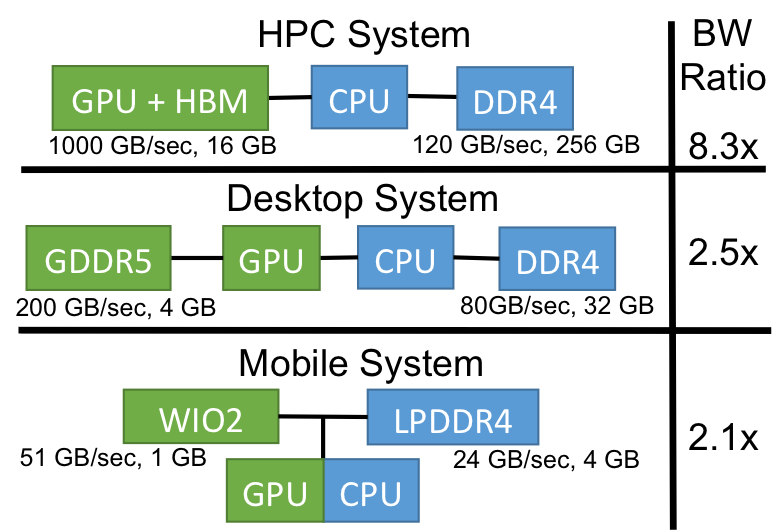
\includegraphics[width=\columnwidth]{asplos2015/figures/arch}
    \caption{BW-Ratio of high-bandwidth vs high-capacity memories for likely future HPC, desktop, and mobile systems}
    \label{fig:arch}
\end{figure}

%To date, GPU-attached bandwidth optimized (BO) memory has been allocated and
%managed primarily as the result of explicit, programmer-directed function calls.
%As heterogeneous GPU/CPU systems move to a transparent unified memory system,
%the OS and runtime systems will become increasingly responsible for memory
%management functions such as page placement, just as they are in CPU-only NUMA
%systems today. In CC-NUMA systems, the notion of local versus remote memory
%latency is exposed to the operating system via the Advanced Configuration and
%Power Interface (ACPI). The latency differences between local and remote memory
%account for the additional latency incurred due to accessing remote memory
%across the system interconnect.  In these systems, latency information, alone,
%is adequate, as CPUs are generally more performance sensitive to memory system
%latency, rather than other memory characteristics.

Massively parallel GPUs and their highly-threaded programming models can
tolerate long memory latencies but, these throughput oriented processors demand
high bandwidth. However, due to lack of exposure of difference in bandwidth
capabilities differential of main memory technologies OS or the programmer, they
cannot make the best memory management decisions to exploit the memory bandwidth
of heterogeneous CPU-GPU system. In this thesis we explore the effect on GPU
performance of exposing memory system bandwidth information to the operating
system/runtime and user applications to improve the quality of dynamic page
placement decisions.

We explore two OS page placement policies:\\
1) Application agnostic Bandwidth-Aware (BW-AWARE) page placement policy that
can outperform Linux's current bandwidth-optimized INTERLEAVE placement by 35\%
and the default latency optimized LOCAL allocation policy by as much as 18\%,
when the application footprint fits within bandwidth-optimized memory capacity.  
\\
2) For \emph{memory capacity constrained} systems (i.e. bandwidth-optimized memory
capacity is insufficient for the workload footprint), we demonstrate that using
simple application annotations to inform the OS/runtime of hot versus
cold data structures can outperform the current Linux
INTERLEAVE and LOCAL page placement policies.  Our annotation
based policy combined with bandwidth information can outperform these
page placement policies by 19\% and 12\% respectively, and get within
90\% of oracle page placement performance.

%Contributions of this work include:
%
%\begin{enumerate}
%\item
%We show that existing CPU-oriented page placement policies are not only 
%sub-optimal for placement in GPU-based systems, but simply do not have the 
%appropriate information available to make informed decisions when optimizing for 
%bandwidth-asymmetric memory.  Exposing additional bandwidth information 
%to the OS, as is done for latency today, will be required for optimized decision 
%making.
%\item 
%Perhaps counter-intuitively we show that, placing all pages in the 
%bandwidth optimized memory is not the best performing page placement 
%policy for GPU workloads.  We propose and {\color{black}simulate} a new bandwidth-aware (BW-AWARE) page 
%placement policy that can outperform Linux's current bandwidth-optimized 
%INTERLEAVE placement by 35\% and the default latency optimized LOCAL allocation 
%policy by as much as 18\%, when the application footprint fits 
%within bandwidth-optimized memory capacity.  
%\item 
%For \emph{memory capacity constrained} systems (i.e. bandwidth-optimized memory
%capacity is insufficient for the workload footprint), we demonstrate that using
%simple application annotations to inform the OS/runtime of hot versus
%cold data structures can outperform the current Linux
%INTERLEAVE and LOCAL page placement policies.  Our annotation
%based policy combined with bandwidth information can outperform these
%page placement policies by 19\% and 12\% respectively, and get within
%90\% of oracle page placement performance.
%\end{enumerate}

%%\vspace{-0.05in}
\section{Motivation and Background}
\label{background}
%\vspace{-0.05in}

\subsection{{Heterogeneous CC-NUMA Systems}}
\label{heterogeneous_background}
%\vspace{-0.05in}
Systems using heterogeneous CPU and GPU computing resources
have been widely used for several years.  Until recently, the GPU 
has been managed as a separate accelerator, requiring 
explicit memory management by the programmer to transfer data to and 
from the GPU's address space and (typically) the GPU's locally-attached
memory.  To increase programmer productivity and broaden the classes
of workloads that the GPU can execute, recent systems have introduced
automatic memory management enabling the CPU and GPU to access a unified
address space and transparently migrate data at a page-level 
granularity~\cite{UVM}.
The next step in this evolution is making the GPU a cache-coherent peer
to the CPU in the memory system, which is the stated goal of a number
of commercial vendors~\cite{HSA}.

\begin{figure}[t]
    \subfloat[Bandwidth sensitivity] {
        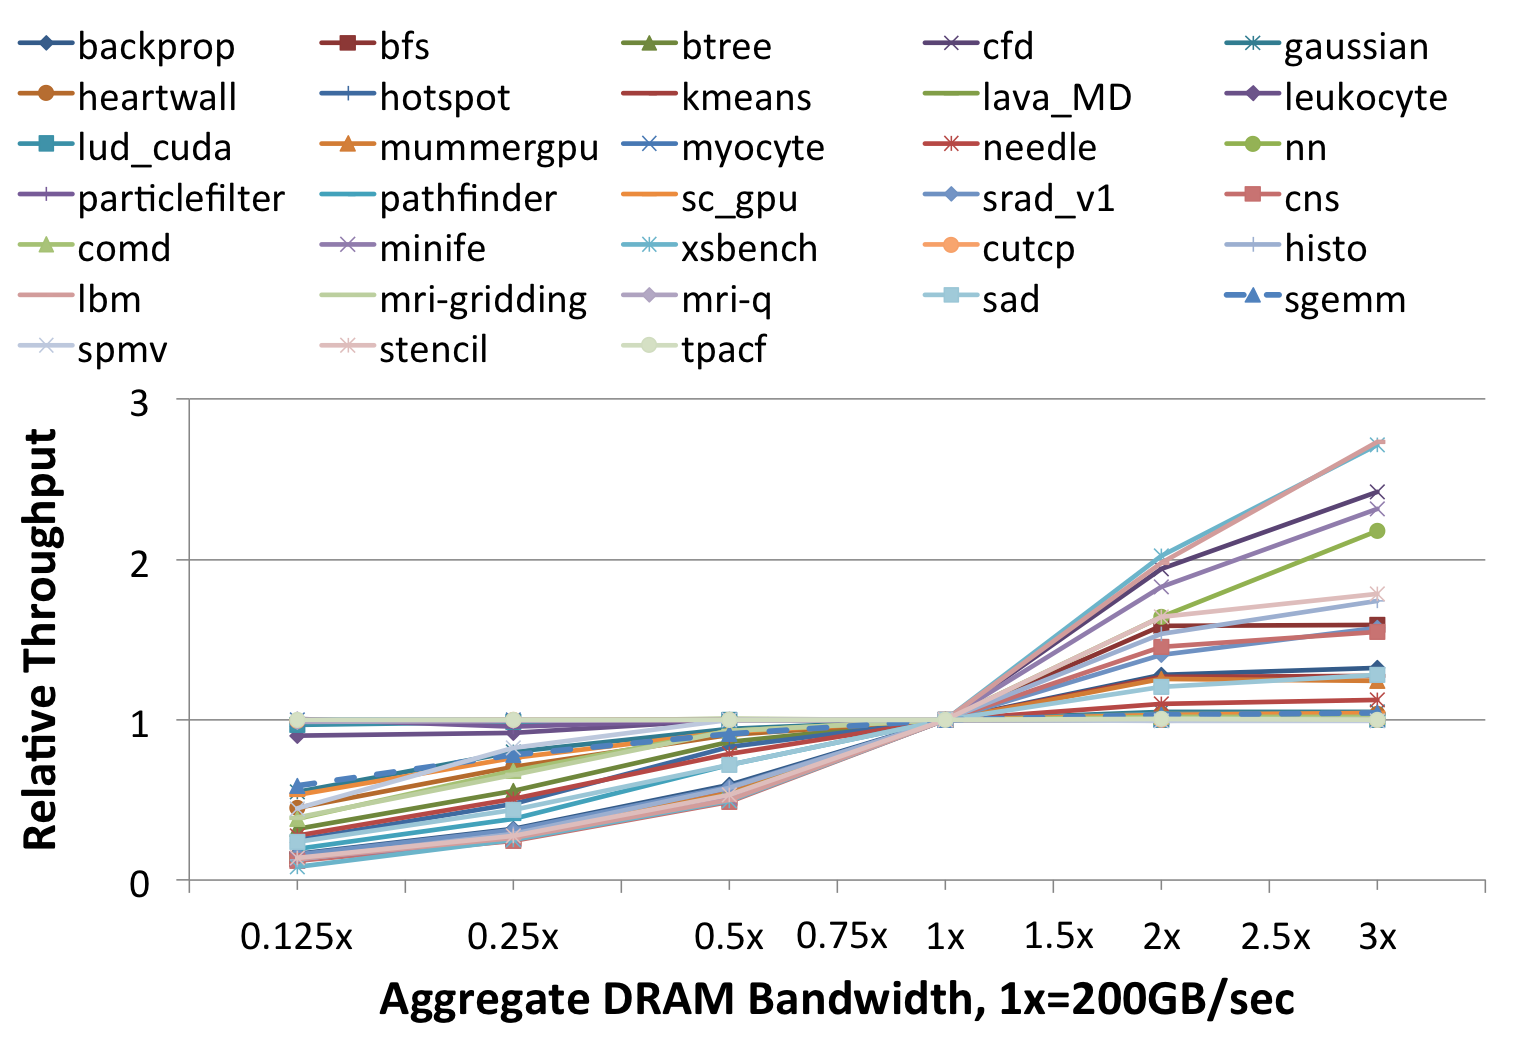
\includegraphics[width=\columnwidth]{asplos2015/figures/bandwidth-1.png}
        \label{fig:bandwidth}
    }
    \\
    \subfloat[Latency sensitivity] {
        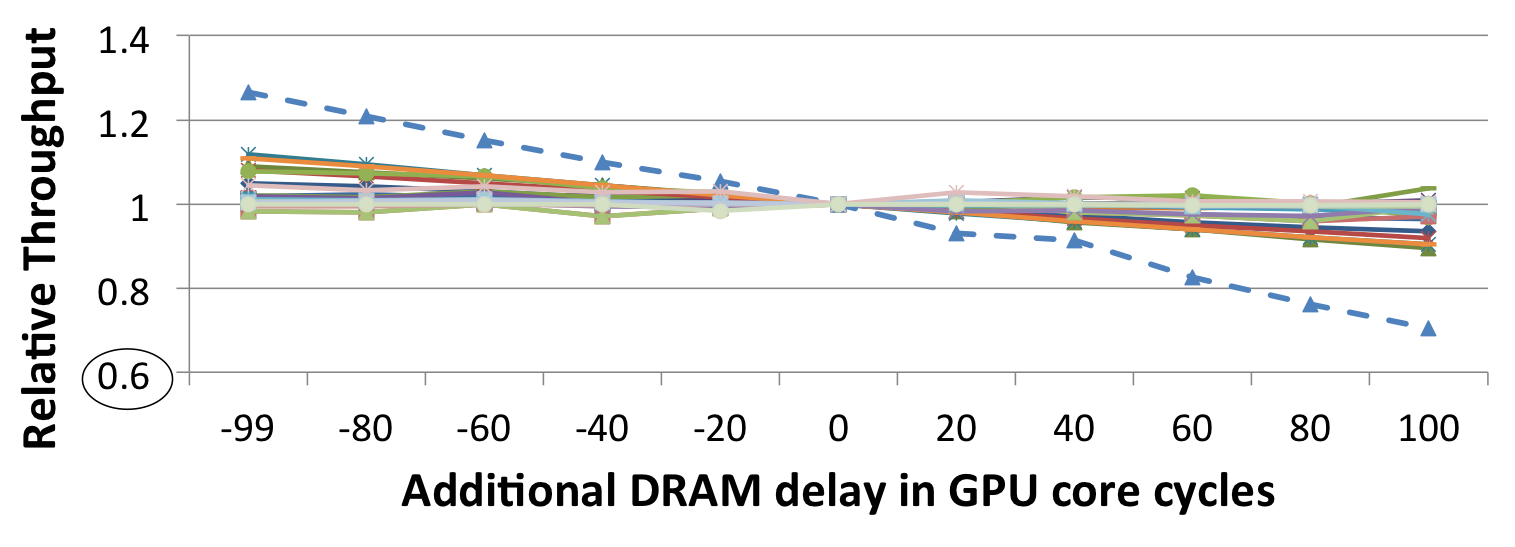
\includegraphics[width=\columnwidth]{asplos2015/figures/latency-1.png}
        \label{fig:latency}
    }
    \caption{GPU performance sensitivity to bandwidth and latency changes.}
    \label{fig:bwlatencysensitivity}
\end{figure}

While some heterogeneous CPU/GPU systems share a single unified physical memory~\cite{AMDAPU},
discrete GPUs are already using specialized DRAM optimized to meet their high bandwidth demands.  
To highlight the sensitivity of GPU performance to memory characteristics, Figures~\ref{fig:bandwidth} and~\ref{fig:latency} show the
performance variation as memory bandwidth and latency vary for a variety of GPU compute benchmarks from the
Rodinia~\cite{Che2009} and {\color{black}Parboil~\cite{Parboil} suites, as well as a number of recent HPC~\cite{comd,cns,minife,xsbench}
workloads. Most of these GPU workloads are
sensitive to changes in bandwidth, while showing much more modest
sensitivity to varying the latency; only {\tt sgemm} stands
out as highly latency sensitive among these 33 workloads. Some application kernels are
neither bandwidth nor latency sensitive and do not see significant performance variation
as modifications are made to the memory subsystem.} While GPU-equipped systems generally require bandwidth-optimized memories to achieve peak performance,
these memory technologies have significant cost, capacity, and/or energy disadvantages over alternative DRAM technologies.

The most common bandwidth-optimized (BO) memory technology today is GDDR5~\cite{GDDR5}.  Providing a per-pin
data rate of up to 7Gbps, this memory technology is widely used with discrete GPUs used in HPC,
workstation, and desktop systems.  Due to the high data rates, GDDR5 systems require significant energy per access
and are unable to support high-capacity multi-rank systems.
In contrast, the roadmap for the next several years of cost/capacity-optimized (CO) DRAM (DDR4 and LPDDR4) 
provides a per-pin data rate that reaches only 3.2 Gbps.  However, these CO DRAM technologies provide similar latency at 
a fraction of the cost and lower energy per access compared to the BO GDDR5 memories.
Looking forward, systems requiring more bandwidth and/or reduced energy per access are moving to  
die-stacked DRAM technologies~\cite{HBM,WIDEIO2}.  These bandwidth-optimized stacked memories are 
significantly more energy-efficient than off-package memory technologies like GDDR5, DDR4, and LPDDR4.  
Unfortunately, the number of DRAM die that can be economically stacked in a single package is limited, 
necessitating systems to also provide a pool of off-package capacity-optimized DRAM.

This disaggregation of memory into on-package and off-package pools is one factor motivating
the need to revisit page placement within the context of GPU performance.  Future GPU/CPU systems are 
likely to take this disaggregation further and move capacity-optimized memory not 
just off the GPU package, but across a high speed interconnect where it is physically attached to the CPU
rather than the GPU, or possibly further~\cite{Lim2009}.  
In a CC-NUMA system, the physical location of this capacity-optimized memory only changes the latency and bandwidth
properties of this memory pool -- it is functionally equivalent regardless of being CPU or GPU locally attached.  A robust
page placement policy for GPUs will abstract the on-package, off-package, and remote memory properties into
performance and power characteristics based on which it can make optimized decisions.

\subsection{Current OS NUMA Page Placement}
\label{linux_background}
%\vspace{-0.05in}
In modern symmetric multiprocessor (SMP) systems, each socket typically
consists of several {\color{black}cores} within a chip multi-processor (CMP) that share 
last-level caches and on-chip memory controllers~\cite{INTELXEON}. The number of
memory channels connected to a processor socket is often limited by the
available pin count.  To increase the available memory bandwidth and capacity 
in a system, individual sockets can be connected via a cache coherent interconnect 
fabric such as Intel's Quick Path~\cite{INTELQPI}, AMD's HyperTransport~\cite{AMDHT},
or NVIDIA's NVLink~\cite{NVLINK}.  A single socket, the processors
within it, and the physically attached memory comprise what an operating system
sees as a local NUMA zone.  Each socket is a separate NUMA zone. While a
processor within any given zone can access the DRAM within any other zone, there
is additional latency to service this memory request compared to a locally
serviced memory request because the request must be routed first to its
own memory controller, across the socket interconnect, and through the remote
memory controller.

Operating systems such as Linux have recognized that, unless necessary, it is
typically better for applications to service memory requests from their own
NUMA zone to minimize memory latency.  To get the best performance out of these NUMA
systems, Linux learns system topology information from the Advanced Configuration
and Power Interface (ACPI) System Resource
Affinity Table (SRAT) and memory latency information from the ACPI 
System Locality Information Table (SLIT)\@. After discovering this information,
Linux provides two basic page placement policies that can be specified by 
applications to indicate where they prefer their physical memory pages to be placed
when using standard {\tt malloc} and {\tt mmap} calls to allocate memory.

\emph{LOCAL:} The default policy inherited by user processes is
\emph{LOCAL} in which physical page allocations will be from memory within the 
local NUMA zone of the executing process, unless otherwise specified or due to capacity
limitations.  This typically results in allocations from memory
physically attached to the CPU on which the process is running, thus minimizing
memory access latency.

\emph{INTERLEAVE:} The second available allocation policy, which processes
must specifically inform the OS they would like to use, is \emph{INTERLEAVE}\@. This
policy allocates pages round-robin across all (or a subset)
of the NUMA zones within the SMP system to balance bandwidth across the memory pools.
The downside of this policy is that the additional bandwidth comes at the expense of
increased memory latency. Today, the OS has no knowledge about the relative 
bandwidth of memories in these different NUMA zones because SMP
systems have traditionally had bandwidth-symmetric memory systems.

In addition to these OS placement policies, Linux provides a library interface called \textit{libNUMA}
for applications to request memory allocations from
specific NUMA zones.  This facility provides low-level control over memory placement
but requires careful programming because applications running on different systems will often have
different NUMA-zone layouts.  Additional difficulties arise because there is no performance
feedback mechanism available to programmers when making memory placement decisions, nor are they
aware of which processor(s) their application will be running on while writing their application.

With the advent of heterogeneous memory systems, the assumptions
that operating system NUMA zones will be symmetric in bandwidth, latency, and power characteristics break down.  
The addition of heterogeneous GPU and CPU computing resources further stresses the page placement
policies since processes may not necessarily be migrated to help 
mitigate performance imbalance, as 
certain phases of computation are now pinned to the type of processor executing the program.
As a result, data placement policies combined with bandwidth-asymmetric
memories can have significant impact on GPU, and possibly CPU, performance.

% move related work up to the background and motivation
\subsection{Related Work}
\label{related_work}
%\vspace{-0.05in}
With the introduction of symmetric multiprocessors, significant work has examined optimal placement of processes and memory
in CC-NUMA systems~\cite{Wilson2001,Bolosky1989,Brecht1993,LaRowe1992,Verghese1996,Iyer1998}.
While much of this early work focused on placing processes and data in
close proximity to each other,  more recent work has recognized that
sharing patterns, interconnect congestion, and even queuing
delay within the memory controller are important metrics to consider when
designing page and process placement policies~\cite{AUTONUMA,Dashti2013,Tam2007,Zhuravlev2010,Knauerhase2008,Blagodurov2011,awasthinellans10}.
Nearly all of these works focus on improving traditional CPU throughput
where reduced memory latency is the primary driver of memory system performance.
Recent work from Gerofi et al.~\cite{Gerofi2014} examines TLB replacement policies for the Xeon Phi
co-processor with a focus on highly parallel applications with large data
footprints.

Using non-DRAM technologies or mixed DRAM technologies for main memory systems to improve power
consumption on traditional CPUs has also been
explored by several groups~\cite{Kultursay2013,Phadke11mlpaware2011,Mogul2009,Bheda2011,Ramos2011,Nil2012,pavlovic2013}.  
Much of this work has focused on overcoming the performance
peculiarities that future non-volatile memory (NVM) technologies may have compared to existing DRAM designs.
In addition to mixed technology off-package memories, upcoming on-package memories provide opportunities
for latency reduction by increasing the number of banks available to the application~\cite{Dong2010}
and may one day be configurable to balance bandwidth application needs with power
consumption~\cite{Zhao2012}.
An alternative to treating heterogeneous memory systems as a flat
memory space is to use one technology as a cache for the other~\cite{jiang2011,Meza2012}.  While this
approach has the advantage of being transparent to the programmer, 
{\color{black}OS, and runtime systems}, 
few implementations~\cite{Sim2012} take advantage of the additive bandwidth available
when using heterogeneous memory.

In the GPU space, Zhao et al.~\cite{zhao2013} have explored the affect 
of hybrid DRAM-NVM systems on GPU compute workloads, making the observation that modern GPU designs are very
good at hiding variable memory system latency. Wang et al.~\cite{Wang2013} explore a mixed NVM-DRAM
system that uses compiler analysis to identify near-optimal data placement across kernel invocations
for their heterogeneous memory system. While their system 
does not significantly improve performance, it offers improved power 
efficiency through use of NVM memory and shows that software based page 
placement, rather than hardware caching, can be a viable 
alternative to managing heterogeneous memory for use with GPUs.


%\vspace{-0.05in}
\section{BW-AWARE Page Placement}
\label{bwawareplacement}
%\vspace{-0.05in}
Using all available memory bandwidth is a key driver to maximizing 
performance for many GPU workloads.
To exploit this observation, we propose a new OS page placement algorithm which
accounts for the bandwidth differential between different bandwidth-optimized and 
capacity-optimized memories
when making page placement decisions.  This section discusses the need,
implementation, and results for a bandwidth-aware (BW-AWARE) page placement
policy for systems where the application footprint fits within BO memory, the
common case for GPU workloads today.  Later in Section~\ref{binaryinstrument},
we discuss an extension to BW-AWARE placement for systems where memory placement
decisions are constrained by the capacity of the
bandwidth-optimized memory.  Both HPC systems trying to maximize in-memory
problem footprint and mobile systems which are capacity limited by cost and
physical part dimensions may soon encounter these capacity constraints with
heterogeneous memories.

\subsection{Bandwidth Maximized Page Placement}
\label{unconstrained}
%\vspace{-0.05in}
The goal of bandwidth-aware page placement is to enable a GPU
to effectively use the total combined bandwidth of {\color{black}\emph{all} the} memory in the
system.  Because GPUs are able to hide high memory latency without stalling
their pipelines, all memories in a system can be used to service GPU requests, 
even when those memories are off-package or require one or more hops
through a system interconnect to access.
To exploit bandwidth-heterogeneous memories,
our BW-AWARE policy places physical memory pages in the ratio of aggregate 
bandwidths of the memories in the system without requiring any knowledge of page
access frequency. Below we derive that this placement policy is optimal for maximizing
bandwidth.

Consider a system with bandwidth-optimized and capacity-optimized
memories with bandwidths $b_B$ and $b_C$ respectively, where unrestricted
capacity of both memories are available. Let $f_B$ represent fraction of data
placed in the BO memory and $1-f_B$ in the CO memory.  Let us assume there are total of
N memory accesses uniformly spread among different pages. Then the total amount
of time spent by the BO memory to serve $N*f_B$ memory accesses is $N*f_B/b_B$ and
that by the CO memory to serve $N(1-f_B)$ memory accesses is $N(1-f_B)/b_C$.  Since
requests to these two memories are serviced in parallel, the total time T to serve the
memory requests is: 
%\[
%T=max(N*f_B/b_B, N(1-f_B)/b_C)
%\]
$$T=max(N*f_B/b_B, N(1-f_B)/b_C)$$
To maximize performance, T must be minimized. Since, $N*f_B/b_B$ and
$N(1-f_B)/b_C$ are linear in $f_b$ and $N*f_B/b_B$ is increasing function while
$N(1-f_B)/b_C$ is decreasing, the minimum of T occurs when both are equal:
%\[T_{opt}=N*f_B/b_B = N(1-f_B)/b_C\]
$$T_{opt}=N*f_B/b_B = N(1-f_B)/b_C$$
Therefore,
%\[f_{Bopt}=b_B/(b_B+b_C)\]
$$f_{Bopt}=b_B/(b_B+b_C)$$

Because we have assumed that all pages are accessed uniformly, the optimal page
placement ratio is the same as the bandwidth service ratio between the bandwidth-optimized
and capacity-optimized memory pools. From this derivation we make two additional
observations.  First, BW-AWARE placement will generalize to an optimal policy
where there are more than two technologies by placing pages in the bandwidth ratio
of all memory pools. Second, a practical implementation
of a BW-AWARE policy must be aware of the bandwidth provided by the various
memory pools available within a system. Hence there is a need for a new System
Bandwidth Information Table (SBIT), much like there is already a ACPI System
Locality 
Information Table (SLIT) which exposes memory latency information to the operating
system today. We will re-visit the assumption of uniform page access later in Section~\ref{annotation}.  

\begin{table}[t]
\begin{center}
\begin{small}
\begin{tabular}{|l|l|}
%\hline
%Simulator & GPGPU-Sim 3.x\\
%\hline
%GPU Arch & NVIDIA GTX-480 Fermi-like\\
%\hline
%GPU Cores& 15 {\color{black}SMs} @ 1.4Ghz\\
%\hline
%L1 Caches & 16kB/SM \\
%\hline
%L2 Caches & Memory Side 128kB/DRAM Channel\\
%\hline
%L2 MSHRs & 128 Entries/L2 Slice\\
%\hline
\hline
\multicolumn{2}{|c|}{Memory system}\\
\hline
GPU-Local GDDR5 & 8-channels, 200GB/sec aggregate\\
\hline
GPU-Remote DDR4& 4-channels, 80GB/sec aggregate\\
\hline
DRAM Timings & \multicolumn{1}{|l|}{RCD=RP=12,RC=40,CL=WR=12}\\
\hline
GPU-CPU &  100 GPU core cycles\\
Interconnect Latency & \\
\hline
\end{tabular}
\caption{Memory system configuration for heterogeneous CPU-GPU system.}
\label{tab:bw-methodology}
\end{small}
\end{center}
\vspace{-0.15in}
\end{table}

\subsection{Experimental Results}
%\vspace{-0.05in}

While it would be ideal to evaluate our page placement policy on a real CC-NUMA
GPU/CPU system with a heterogeneous memory system, such systems are not available today.
Mobile systems containing both ARM CPU cores and NVIDIA GPU cores exist today in products
such as the NVIDIA Shield Portable, but use a single LPDDR3 memory system.
Desktop and HPC systems today have heterogeneous memory attached to CPUs and discrete
GPUs but these processors are not connected through a cache coherent interconnect.  They require explicit user 
management of memory if any data is to be copied from the host CPU memory to the GPU memory or vice versa
over the PCIe interconnect. Pages can not be directly placed into GPU memory on allocation by the operating system.
Without a suitable real system to experiment on, we turned to simulation to evaluate our
page placement improvements.

%\vspace{0.05in}
\subsubsection{Methodology}
To evaluate BW-AWARE page placement, we simulated a heterogeneous memory system
attached to a GPU comprised of both bandwidth-optimized GDDR and
cost/capacity-optimized DDR where the GDDR memory is attached directly to the
GPU\@.  We discuss our baseline simulation environment in
Chapter~\ref{chap:methodology}.
%No contemporary GPU system is available which supports cache-coherent access to
%heterogeneous memories.  Commonly available PCIe-attached GPUs are constrained
%by interconnect bandwidth and lack of cache-coherence; while cache-coherent GPU
%systems, such as AMD's Kaveri, do not ship with heterogeneous memory.  Our
%simulation environment is based on GPGPU-Sim~\cite{gpgpusimIspass09} which has
%been validated against NVIDIA's Fermi class GPUs and is reported to match
%hardware performance with up to 98.3\% accuracy~\cite{gpgpusimManual}.  We
%modified GPGPU-Sim to support a heterogeneous GDDR5-DDR4 memory system with the
%simulation parameters listed in Table~\ref{tab:methodology}.
We model a baseline system with 200GB/s of GPU-attached memory bandwidth and
80GB/s of CPU-attached memory bandwidth, providing a bandwidth ratio of
$2.5\times$\@ as shown in Table~\ref{tab:bw-methodology}.
%We made several changes to the baseline GTX-480 model to bring our
%configuration in-line with the resources available in more modern GPUs,
%including a larger number of MSHRs and higher clock frequency.
With a focus on memory system performance, we evaluate GPU workloads which are
sensitive to memory bandwidth or latency from three benchmark suites:
Rodinia~\cite{Che2009}, Parboil~\cite{Parboil} and recent
HPC~\cite{comd,cns,minife,xsbench} workloads; those which are compute-bound see
little change in performance due to changes made to the memory system.  For the
remainder of the evaluation in this chapter we show results for 19 benchmarks,
17 of which are sensitive to memory bandwidth while also providing {\tt comd}
and {\tt sgemm} results to represent applications which are memory insensitive
and latency sensitive respectively.

%As noted in Section~\ref{heterogeneous_background}, attaching the capacity-optimized memory
%directly to the GPU is functionally equivalent to remote CPU attached memory,
%but with different latency parameters.  To simulate an additional interconnect hop
%to remote CPU-attached memory, we model a fixed, pessimistic, additional 100 cycle latency to access
%the DDR4 memory from the GPU\@. This overhead is derived from the single additional interconnect
%hop latency found in SMP CPU-only designs such as the Intel XEON~\cite{INTELXEON}\@.

%Our heterogeneous memory model contains the same number of MSHRs per memory
%channel as the baseline memory configuration.  The number of MSHRs in the
%baseline configuration is sufficient to effectively hide the additional
%interconnect latency to the DDR memory in Figure~\ref{fig:latency}. Should MSHR
%quantity become an issue when supporting two level memories, previous work has
%shown that several techniques can efficiently increase MSHRs with only modest
%cost~\cite{ref:tuck:scalablemisshandling, ref:minikin:prefetch}.

%Paging model talk
Implementing a BW-AWARE placement policy requires adding another mode ({\tt
MPOL\_BWAWARE}) to the {\tt set\_mempolicy()} system call in Linux\@. When a
process uses this mode, the Linux kernel will allocate pages from the two memory
zones in the ratio of their bandwidths.  These bandwidth ratios may be obtained
from future ACPI resources or dynamically determined by the GPU runtime at
execution time.

\begin{figure}[t]
    \centering
    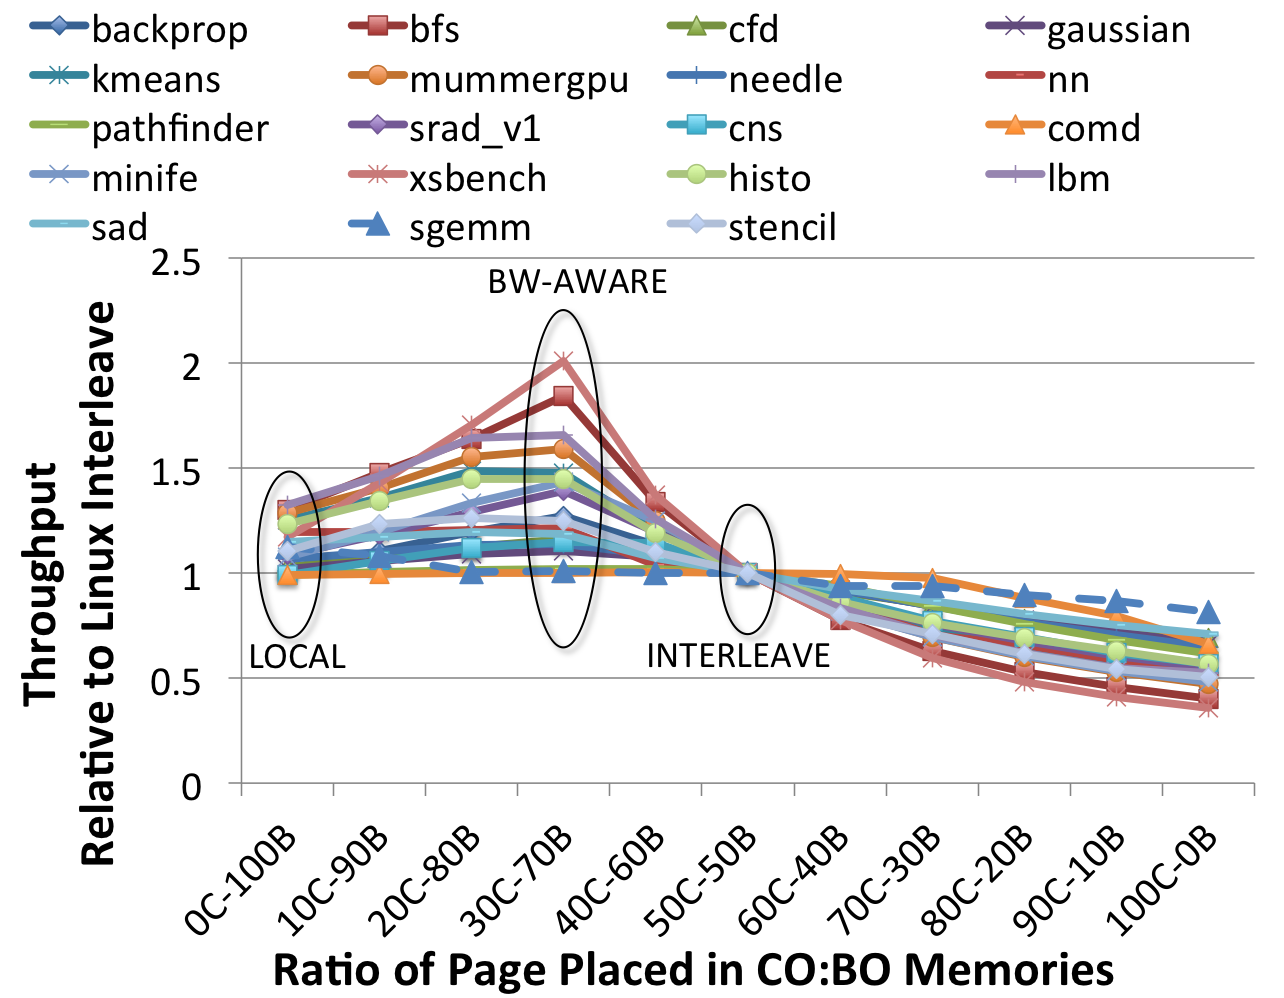
\includegraphics[width=0.9\columnwidth]{asplos2015/figures/bw-aware-2.png} 
    \caption{GPU workload performance with different page placement policies.
$xC$-$yB$ policy represents $x:y$ data transfer ratio from CO and BO memory respectively.}
    \label{fig:baseline}
\end{figure}

%\vspace{0.05in}
\subsubsection{BW-AWARE Performance}
We define our BW-AWARE page placement policy $xC$-$yB$, where $x$ and $y$ denote the
percentage of pages placed in a given memory technology, $C$ stands for capacity-optimized
memory and $B$ stands for bandwidth-optimized memory. By definition $x+y=100$. For our baseline
system with 200GB/sec bandwidth-optimized memory and 80GB/sec of capacity-optimized memory the
aggregate system bandwidth is 280GB/sec.  In this
notation, our BW-AWARE policy will then be $x=80/280=28\%$ and $y=200/280=72\%$, represented as
$28C$-$72B$. However, for simplicity we will round this to $30C$-$70B$ for use as the 
placement policy.  For processes running on the GPU, the LOCAL policy
would be represented as $0C$-$100B$; $50C$-$50B$ corresponds to the bandwidth spreading Linux
INTERLEAVE policy.

To achieve the target $30C$-$70B$ bandwidth ratio, we implemented BW-AWARE placement as follows.
On any new physical page allocation, a random number in the range $[0,99]$
is generated.  If this number is $\geq30$, the page is allocated from the bandwidth-optimized memory; 
otherwise it is allocated in the capacity-optimized memory. A LOCAL allocation policy can avoid the
comparison if it detects either B or C has the value zero.  While this implementation does
not exactly follow the BW-AWARE placement ratio due to the use of random numbers, in practice this 
simple policy converges quickly towards the BW-AWARE ratio.  This approach also requires no history
of previous placements {\color{black} nor makes any assumptions about the frequency of access to pages}, 
minimizing the overhead for making placement decisions which are on the 
software fast-path for memory allocation.

Figure~\ref{fig:baseline} shows the application performance as we vary the ratio of pages placed in 
each type of memory from 100\% BO to 100\% CO\@. 
For all bandwidth-sensitive applications, the maximum performance is
achieved when using the correct BW-AWARE $30C$-$70B$ placement ratio.  We
find that, on average, a BW-AWARE policy performs 18\% better than the Linux
LOCAL policy and 35\% better than the Linux INTERLEAVE policy. However, for latency sensitive
applications, such as {\tt sgemm}, the BW-AWARE policy may perform worse than a LOCAL
placement policy due to an increased number of accesses to higher latency remote
CO memory. The BW-AWARE placement policy suffers a worse case performance degradation of
12\% over the LOCAL placement policy in this scenario.

%This degradation is expected
% since performance degrades by 9\% when the memory latency is 140 cycles
% (Figure~\ref{fig:latency}), which
% is very near to average memory latency (130 cycles = 70\%*100 + 30\%*200).}
%All of the applications we examined appear to be able to tolerate the additional 
%interconnect latency when using a remote capacity-optimized memory.

Because the current Linux INTERLEAVE policy is identical to BW-AWARE for a bandwidth-symmetric
DRAM $50C$-$50B$ memory technology pairing, we believe a BW-AWARE placement policy could simply
replace the current Linux INTERLEAVE policy without having significant negative side
affects on existing CPU or GPU workloads.  Because maximizing bandwidth is more important
than minimizing latency for GPU applications, BW-AWARE placement may be a good candidate
to become the default placement policy for GPU-based applications.
% It is worth noting that there are some GPU applications that are known to be
% sensitive to DRAM latency {\color{red}({\tt sgemm} in our case)}, 
% and using the LOCAL page placement policy may still be preferred.

\begin{figure}[t]
    \centering
    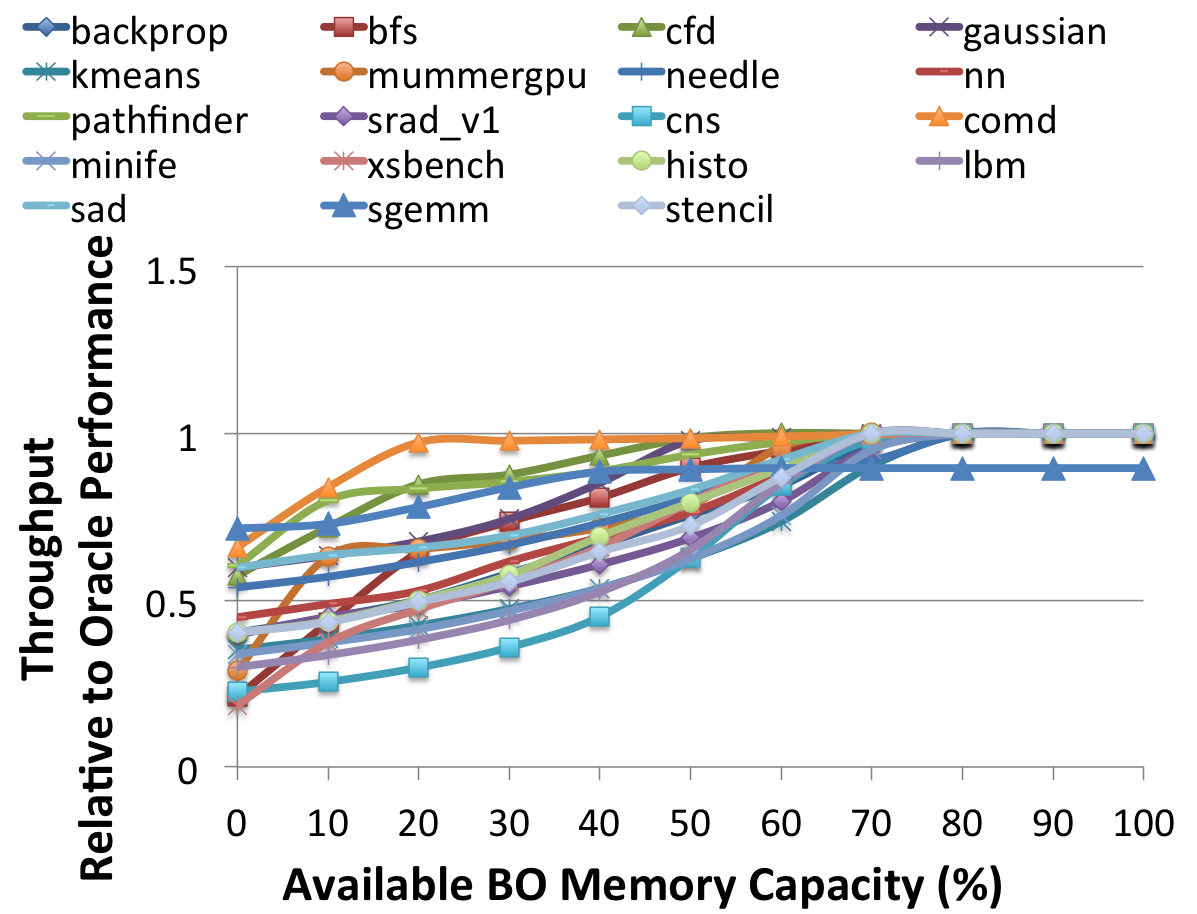
\includegraphics[width=0.9\columnwidth]{asplos2015/figures/bwaware-capacity.png}
    \caption{Performance of BW-AWARE placement as application footprint exceeds
available high-bandwidth
    memory capacity.}
    \label{fig:capacityconstrained}
\end{figure}

%\vspace{0.05in}
\subsubsection{Effective Improvement in Problem Sizing}
Figure~\ref{fig:capacityconstrained} shows the application throughput as we
reduce the capacity of our bandwidth-optimized memory pool as a fraction of the
total application footprint.  BW-AWARE placement is able to achieve near peak
performance even when only 70\% of the application footprint fits within the BO
memory because BW-AWARE placement places only 70\% of pages in BO memory, with
the other 30\% is placed in the less expensive capacity-optimized memory.  Thus,
GPU programmers who today tune their application footprint to fit entirely in
the GPU-attached BO memory could gain an extra 30\% effective memory capacity by
exploiting the CPU-attached CO memory with a BW-AWARE placement policy.
However, as the bandwidth-optimized memory capacity drops to less than 70\% of
application footprint, performance begins to fall off. This effect is due to the
ratio of bandwidth service from the two memory pools no longer matching the
optimal ratio of $30C$-$70B$, with more data being serviced from the capacity
optimized ratio than is ideal. Applications which are insensitive to memory
bandwidth (shown as having little change in Figure~\ref{fig:baseline}), tend to
maintain their performance at reduced capacity points (shown as having little
change in Figure~\ref{fig:capacityconstrained}), because the average bandwidth
reduction does not strongly affect their performance.  Conversely, those
applications with strong BW-performance scaling tend to see larger performance
reduction as the average bandwidth available is reduced, due to capacity
constraints forcing a disproportionate number of memory accesses to the lower
bandwidth CO memory.  The performance at 70\% memory capacity does not exactly
match 100\% of ideal because the actual ratio of bandwidth in our system is
$28C$-$72B$ not $30C$-$70B$.

\begin{figure}[t]
    \centering
    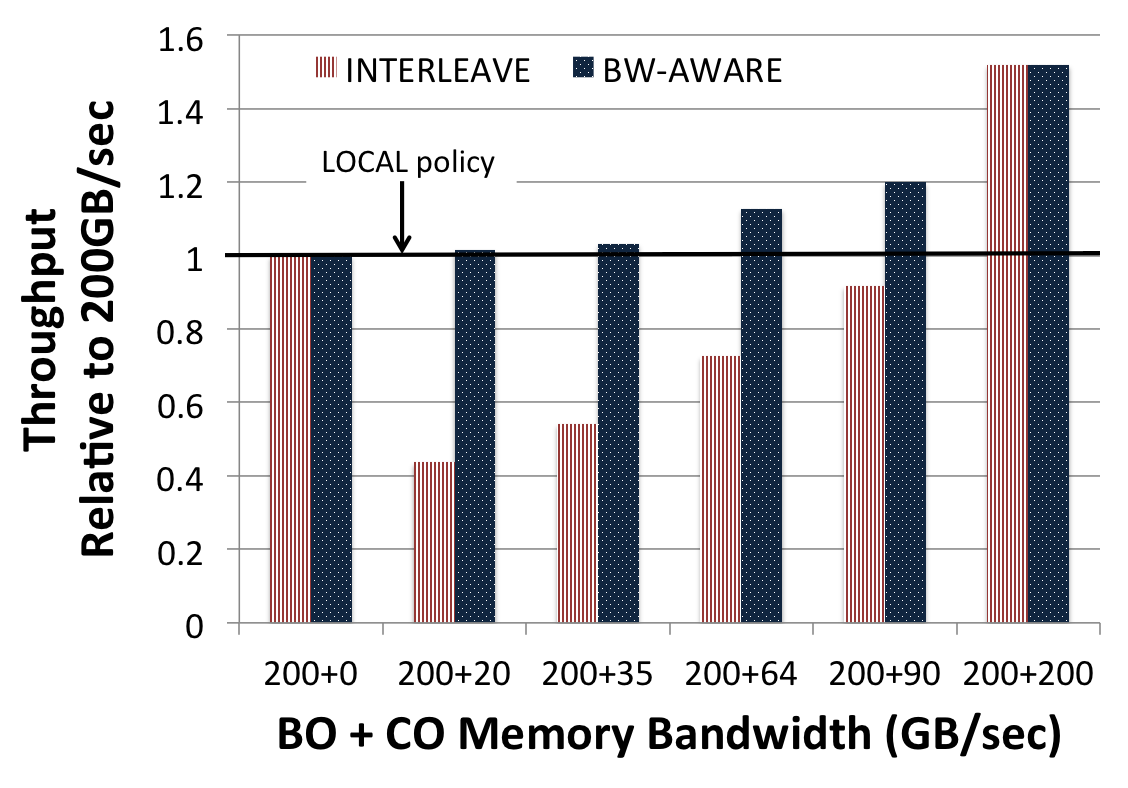
\includegraphics[width=0.9\columnwidth]{asplos2015/figures/sensitivitytobwratio.png}
    \caption{Performance comparison between BW-AWARE, INTERLEAVE, and LOCAL page placement
policies while varying the memory bandwidth ratio.}
    \label{fig:sensitivitytobwratio}
\end{figure}

%\vspace{0.05in}
\subsubsection{Sensitivity to NUMA BW-Ratios} 
Heterogeneous memory systems are likely to come in a variety of configurations.
For example, future mobile products may pair energy efficient and
bandwidth-optimized Wide-IO2 memory with cost-efficient and higher capacity
LPDDR4 memory.  Using the mobile bandwidths shown in
Figure~\ref{fig:arch-asplos2015}, this configuration provides an additional 31\%
in memory bandwidth to the GPU versus using the bandwidth-optimized memory
alone.  Similarly, HPC systems may contain GPUs with as many as 4 on-package
bandwidth-optimized HBM stacks and high speed serial interfaces to bulk capacity
cost/capacity-optimized DDR memory expanders providing just 8\% additional
memory bandwidth.  While we have explored BW-AWARE placement in a desktop-like
use case, BW-AWARE page placement can apply to all of these configurations.  

Figure~\ref{fig:sensitivitytobwratio} shows the average performance of BW-AWARE, INTERLEAVE, and LOCAL
placement policies as we vary the additional bandwidth available from the
capacity-optimized
memory from 0GB/s--200GB/s.
As the bandwidth available from capacity-optimized memory increases, the LOCAL policy
fails to take advantage of it by neglecting to allocate any pages in the capacity-optimized memory.
The Linux INTERLEAVE policy, due to its fixed round-robin allocation, loses performance
in many cases because it oversubscribes the capacity-optimized memory, resulting in less
total bandwidth available to the application.  On the other hand, BW-AWARE placement
is able to exploit the bandwidth from the capacity-optimized memory regardless the 
amount of additional bandwidth available.  Because BW-AWARE placement performs identically to
INTERLEAVE for symmetric memory and outperforms it in all heterogeneous cases, we believe that
BW-AWARE placement is a more robust default policy than INTERLEAVE when considering bandwidth-sensitive 
GPU workloads.

%\vspace{-0.05in}
\section{Understanding Application Memory Use}
\label{constrainedcapacity}
%\vspace{-0.05in}

\begin{figure}[t]
    \centering
    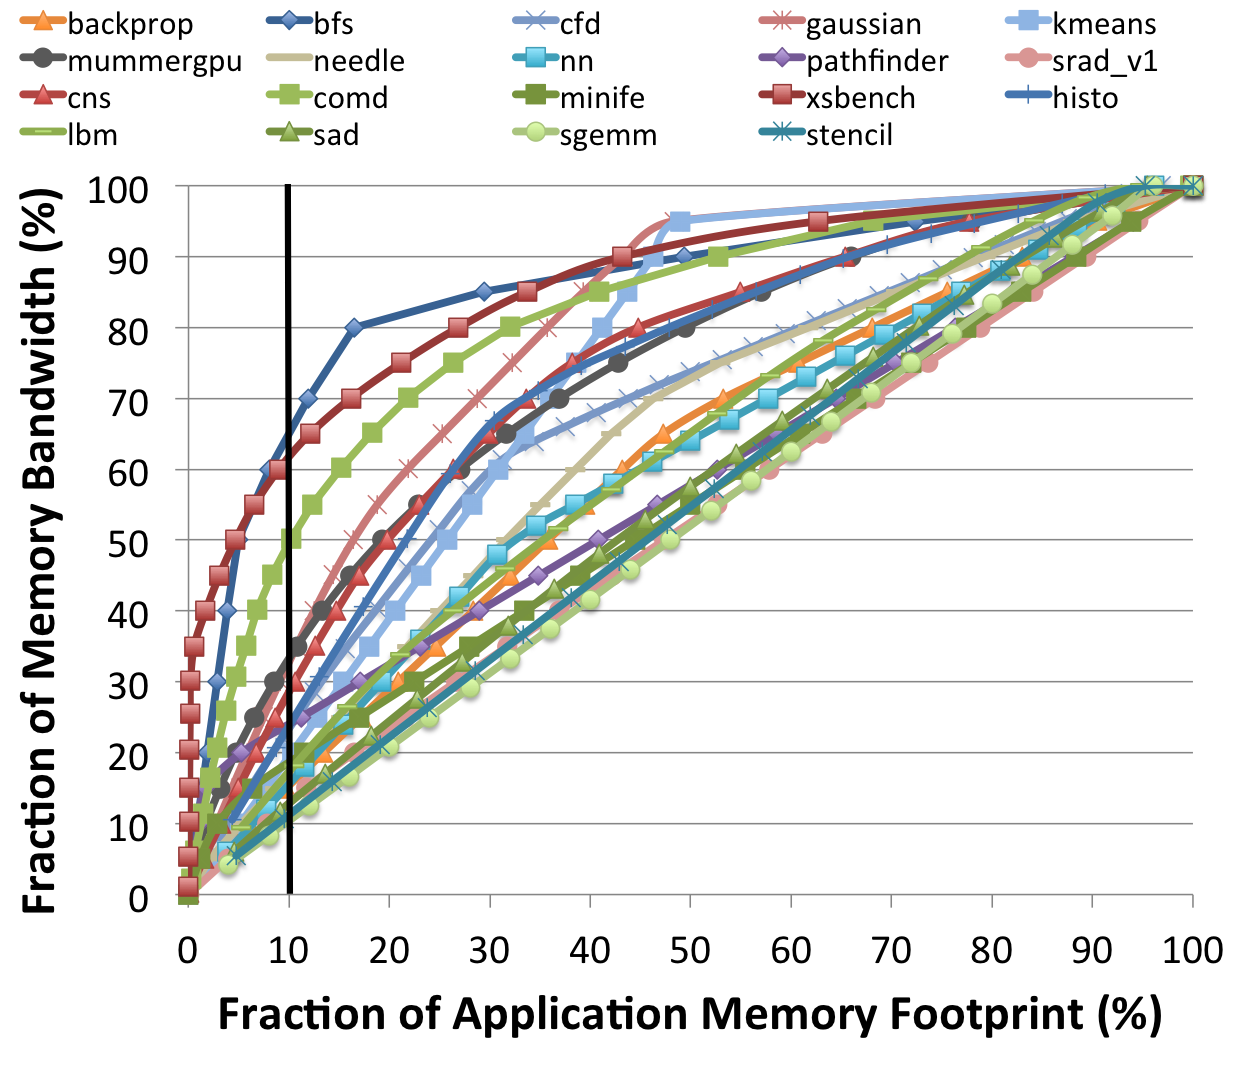
\includegraphics[width=0.9\columnwidth]{asplos2015/figures/cdf.png} 
    \caption{Data bandwidth cumulative distribution function with pages sorted from hot (most memory accesses) to cold (least memory accesses).}
    \label{fig:cdf}
\end{figure}

Section~\ref{bwawareplacement} showed that optimal BW-AWARE placement requires
the majority of the application footprint to fit in the bandwidth-optimized memory
to match the bandwidth service ratios of the memory pools.
However, as shown in Figure~\ref{fig:arch-asplos2015}, systems may have bandwidth-optimized
memories that comprise less than 10\% the total memory capacity, particularly those using
on-package memories which are constrained by physical dimensions. If the application footprint
grows beyond the bandwidth-optimized capacity needed for BW-AWARE placement, the operating system
has no choice but to steer remaining page allocations into the capacity-optimized memory.
Unfortunately, additional pages placed in the CO memory will skew the
ratio of data transferred from each memory pool away from the optimal BW-AWARE ratio.

For example, in our simulated system if the bandwidth-optimized memory
can hold just 10\% of the total application memory footprint, then a BW-AWARE placement would end up placing
10\% pages in the BO memory; the
remaining 90\% pages must be spilled exclusively to the capacity-optimized memory.  This ratio of
$90C$-$10B$ is nearly the inverse of the performance-optimized ratio of $30C$-$70B$.  
To improve upon this capacity-induced placement problem, we recognize
that not all pages have uniform access frequency, and we can selectively place
hot pages in the BO memory and cold pages in the CO memory. 
{\color{black}In this work we define page \textit{hotness} as the number of accesses to that page that 
are served from DRAM.}


\subsection{Visualizing Page Access Distribution}
\label{annotation}
%\vspace{-0.05in}
Figure~\ref{fig:cdf} shows the cumulative distribution function (CDF) 
for memory bandwidth as a fraction of the total
memory footprint for each of our workloads. The CDF was generated by counting
accesses to each 4kB page, after being filtered by on-chip caches, and then sorting
the pages from greatest to least number of accesses.
Applications that have the same number of accesses to all
pages have a linear CDF, whereas applications in which some pages are accessed
more than others have a non-linear CDF skewed towards the left of the
graph. For example, we see that for applications like {\tt bfs} and {\tt xsbench}, over 60\% of
the memory bandwidth stems from within only 10\% of the application's allocated pages.  Skewing the 
placement of these hot pages towards bandwidth-optimized memory will improve the performance
of GPU workloads which are capacity constrained by increasing the traffic to the bandwidth-optimized 
memory. However, for applications which have linear CDFs, there is little headroom for 
improved page placement over BW-AWARE placement.

\begin{figure}[t]
    \centering
    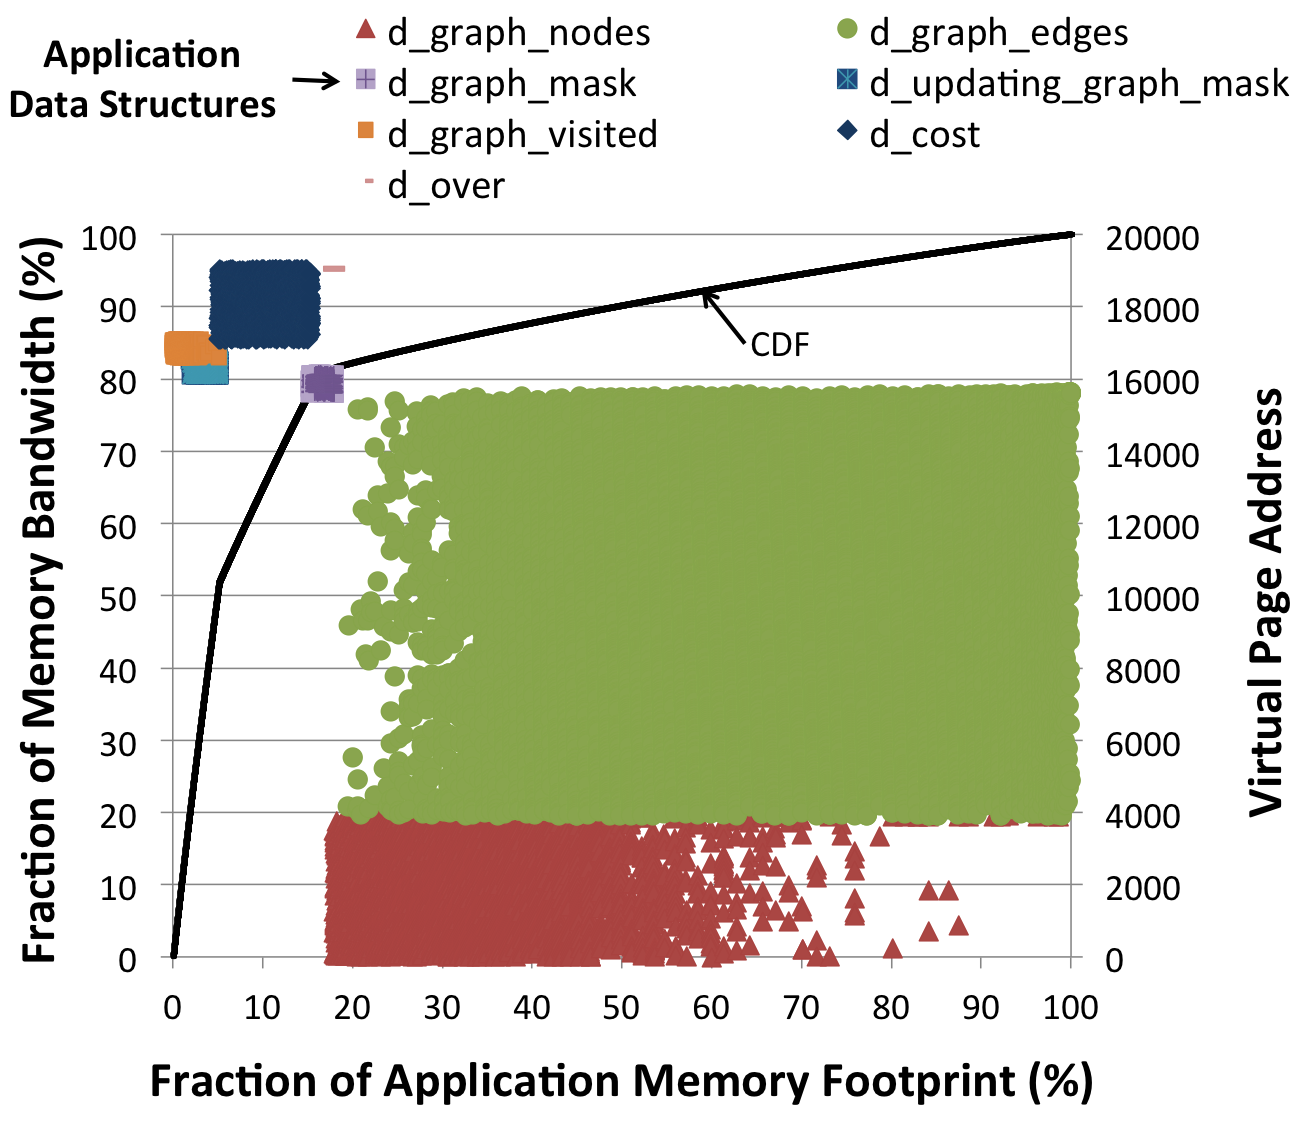
\includegraphics[width=0.9\columnwidth]{asplos2015/figures/bfsannotated.png}
    \caption{{\tt bfs}: CDF of data footprint versus virtual address data layout.}
    \label{fig:cdfannotation-bfs}
\end{figure}

Figure~\ref{fig:cdf} also shows that some workloads have sharp inflection points
within the CDF, indicating that distinct ranges of physical addresses appear to
be clustered as hot or cold. To determine if these inflection points could be
correlated to specific memory allocations within the application, we plotted the
virtual addresses that correspond to application pages in the CDF, and then
reverse-mapped those address ranges to memory allocations for program-level data
structures, with the results shown in
Figure~\ref{fig:cdfannotation-bfs},~\ref{fig:cdfannotation-muumergpu},~\ref{fig:cdfannotation-needle}\@.
{\color{black} The x-axis shows the fraction of pages allocated by the
application, where pages are sorted from greatest to least number of accesses.
The primary y-axis (shown figure left) represents the CDF of memory bandwidth
among the pages allocated by the application (also shown in
Figure~\ref{fig:cdf}).  Each point on the secondary scatter plot (shown figure
right) shows the virtual address of the corresponding page on the x-axis. The
points (pages) are colored according to different data structures they were
allocated from in the program source.}

\begin{figure}[t]
    \centering
    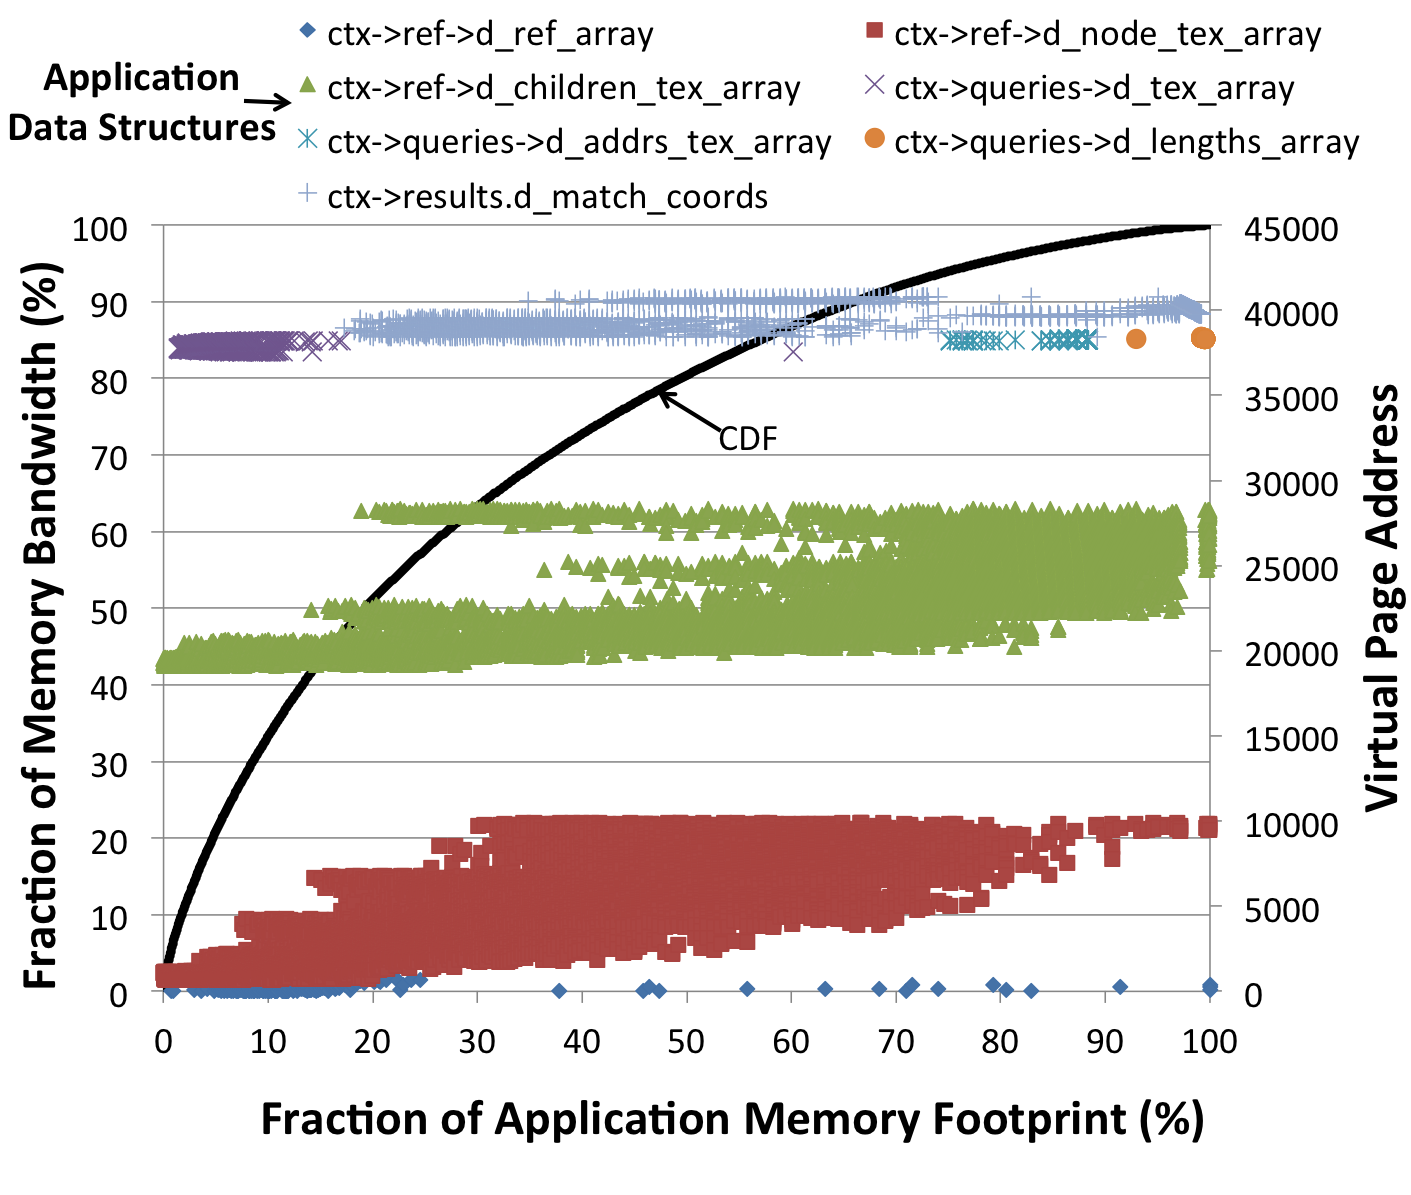
\includegraphics[width=0.9\columnwidth]{asplos2015/figures/mummerannotated.png}
    \caption{{\tt mummergpu}: CDF of data footprint versus virtual address data layout.}
    \label{fig:cdfannotation-muumergpu}
\end{figure}

We analyze three example applications, {\tt bfs, mummergpu}, and
{\tt needle} which show different memory access patterns. For {\tt bfs}, we can
see three data structures: {\tt d\_graph\_visited}, {\tt
d\_updating\_graph\_mask}, and {\tt d\_cost} consume {\color{black}$\approx80\%$
of the total application bandwidth while accounting for $\approx20\%$} of the
memory footprint.  However for {\tt mummergpu}, the memory hotness does not seem
to be strongly correlated to any specific application data structures. Several
sub-structures have similar degrees of hotness and some virtual address ranges
(10,000-19,000 and 29,000-37,000) are allocated but never never accessed. In
{\tt needle}, which has a fairly linear CDF, the degree of memory hotness
actually varies within the same data structure. While we examined all
applications with this analysis, we summarize our two key observations.

\begin{figure}[t]
    \centering
    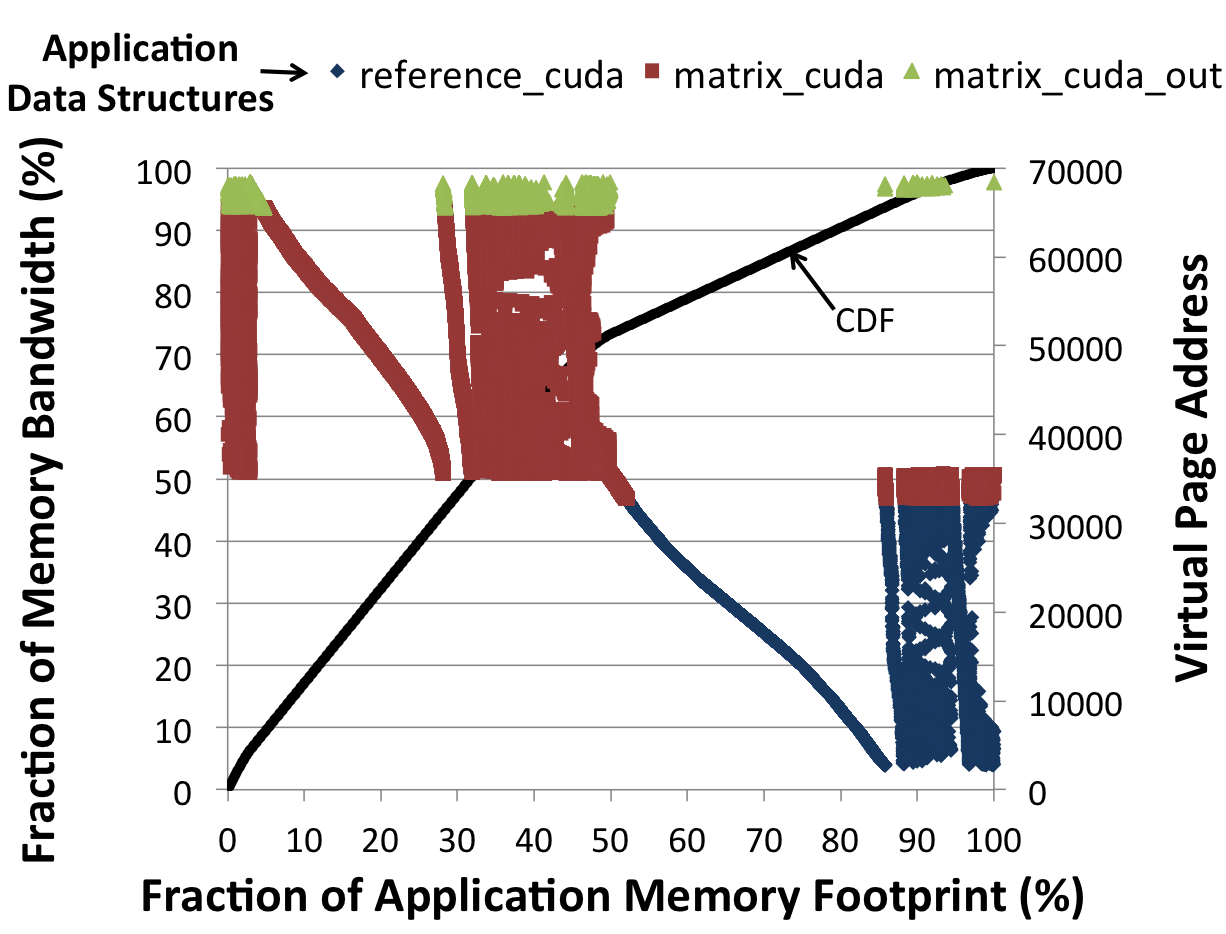
\includegraphics[width=0.9\columnwidth]{asplos2015/figures/needleannotated.png}
    \caption{{\tt needle}: CDF of data footprint versus virtual address data layout.}
    \label{fig:cdfannotation-needle}
\end{figure}

\emph{Individual pages can and often do have different degrees of hotness}.
Application agnostic page placement policies, including BW-AWARE placement, may leave performance 
on the table compared to a placement policy that is aware of page frequency distribution. 
Understanding the relative hotness of pages
is critical to further optimizing page placement.  If an application does not have a skewed CDF, 
then additional effort to characterize and exploit hotness differential will only introduce 
overhead without any possible benefit.

\emph{Workloads with skewed cumulative distribution functions often have sharp
distinctions in page access frequency that map well to different application 
data structures.}  Rather than attempting to detect and segregate individual physical pages 
which may be hot or cold, application structure and memory allocation policy
will likely provide good information about pages which will have similar degrees of hotness.

\subsection{Oracle Page Placement}
With knowledge that page accesses are highly differentiated for some applications, we implemented
an oracle page placement policy to determine how much more application performance could be achieved
compared to BW-AWARE placement in capacity constrained situations.  {\color{black}Using perfect knowledge of page
access frequency, an oracle page placement policy will allocate the hottest pages possible into the
bandwidth-optimized memory until the target bandwidth ratio is satisfied, or the capacity of this memory
is exhausted.}  We implemented this policy using two phase simulation. First, we obtained perfect
knowledge of page access frequency. Then in a second simulation pass, we used this information to allocate
pages to achieve the best possible data transfer ratio under a 10\% capacity constraint where only
10\% of the application memory footprint fits within the bandwidth-optimized memory.

\begin{figure}[t]
    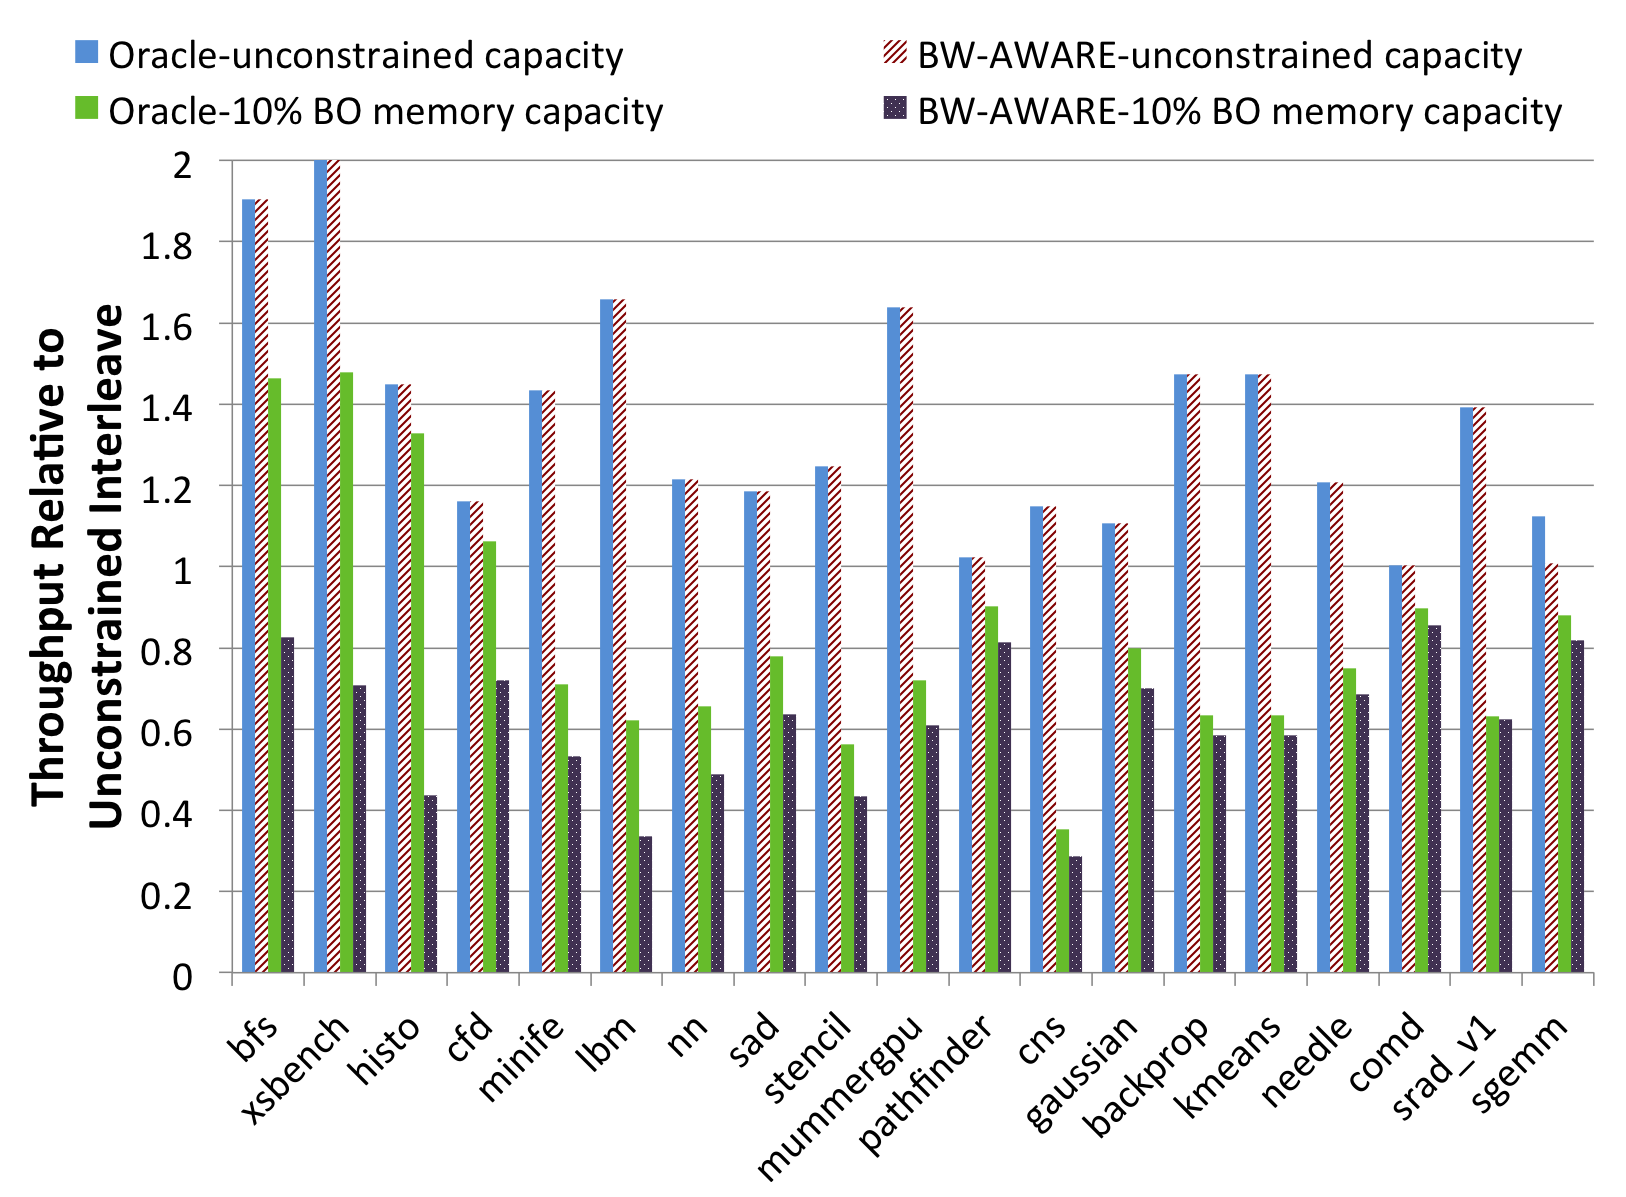
\includegraphics[width=\columnwidth]{asplos2015/figures/oracle-perf.png} 
    \caption{Oracle application performance of a constrained capacity system vs
unconstrained capacity system}
    \label{fig:oracleperf}
\end{figure}

{\color{black}Figure~\ref{fig:oracleperf} compares the performance of the oracle and BW-AWARE
placement policies in both the unconstrained and 10\% capacity constrained
configuration.  Figure~\ref{fig:oracleperf} confirms that BW-AWARE placement is
near-optimal when applications are not capacity limited.  This is because both BW-AWARE
and oracle placement are both able to achieve the ideal bandwidth distribution, though
the oracle policy is able to do this with a smaller memory footprint by placing fewer, hotter, pages in the BO memory.
Under capacity constraints, however, the oracle policy can nearly double the performance of the BW-AWARE policy for applications
with highly skewed CDFs and it outperforms BW-AWARE placement in all cases. This because the random
page selection of BW-AWARE placement is not able to capture enough hot pages for placement in BO
memory, before running out of BO memory capacity, to achieve the ideal bandwidth distribution.  
On average the oracle policy is
able to achieve nearly 60\% the application throughput of a system for which there is no capacity
constraint.  This additional performance, achievable through application awareness of memory
access properties, motivates the need for further improvements in memory placement policy.}

\section{Application Aware Page Placement}
\label{binaryinstrument}
%\vspace{-0.05in}

Figure~\ref{fig:cdfannotation-bfs},~\ref{fig:cdfannotation-muumergpu},~\ref{fig:cdfannotation-needle} 
visually depicts what may be obvious to performance-conscious programmers:
\emph{certain data structures are accessed more frequently than others.} For
these programmers, the unbiased nature of BW-AWARE page placement is not
desirable because all data structures are treated equally.  This section
describes compiler tool-flow and runtime modifications that enable programmers
to intelligently steer specific allocations towards bandwidth- or
capacity-optimized memories and achieve near-oracle page placement performance.

To correctly annotate a program to enable intelligent memory placement decisions
across a range of systems, we need two pieces of information about a program:
(1) the relative memory access hotness of the data structures, and (2) the size
of the data structures allocated in the program.  To understand the importance
of these two factors, let us consider the following scenario. In a program there
are two data structure allocations with hotness H1 and H2\@.  If the
bandwidth-optimized memory capacity is large enough for BW-AWARE placement to be
used without running into capacity constraints, then BW-AWARE page placement
should be used irrespective of the hotness of the data structures. To make this
decision we must know the application runtime memory footprint. However, if the
application is capacity-constrained, then ideally the memory allocation from the
hotter data structure should be preferentially placed in the BO memory. In this
case, we need to know both the relative hotness and the size of the data
structures to optimally place pages.

\subsection{Profiling Data Structure Accesses in GPU Programs}
\label{profiler}
%While GPU programmers have a reputation for deep understanding of their
%application characteristics, as machines become more complex and programs rely
While expert programmers may have deep understanding of their application
characteristics, as machines become more complex and programs rely more on GPU
accelerated libraries, programmers will have a harder time maintaining this
intuition about program behavior.  To augment programmer intuition about memory
access behavior, we developed a new GPU profiler to provide information about
program memory access behavior.  

In this work we augmented {\tt nvcc} and {\tt ptxas}, NVIDIA's
production compiler tools for applications written in CUDA~\cite{cuda} (NVIDIA’s
explicitly parallel programming model), to support data structure access
profiling.  When profiling is enabled, our compiler's code generator emits
memory instrumentation code for all loads and stores that enables tracking of
the relative access counts to virtually addressed data structures within the
program.  As with the GNU profiler {\tt gprof}~\cite{GPROF}, the developer
enables a special compiler flag that instruments an application to perform
profiling.  The developer then runs the instrumented application on a set of
``representative'' workloads, which aggregates and dumps a profile of the
application.  

When implementing this GPU memory profiling tool, one of the
biggest challenges is that {\tt nvcc} essentially generates two
binaries: a host-side program, and a device-side program (that runs on
the GPU).  The profiler's instrumentation must track the execution of
both binaries.  On the host side, the profiler inserts code to track
all instances and variants of {\tt cudaMalloc}.  The instrumentation
associates the source code location of the {\tt cudaMalloc} with the
runtime virtual address range returned by it.  The host side code is
also instrumented to copy this mapping of line numbers and address
ranges to the GPU before each kernel launch.  The GPU-side
code is instrumented by inserting code before each memory operation
to check if the address falls within any of the
ranges specified in the map.  

For each address that falls within a
valid range, a counter associated with the range is incremented, using
atomic operations because the instrumentation code is highly
multi-threaded.  At kernel completion, this updated map is
returned to the host which launched the kernel to aggregate the
statistics about virtual memory location usage. Our profiler generates
informative data structure mapping plots, like those shown in

Figure~\ref{fig:cdfannotation-bfs},~\ref{fig:cdfannotation-muumergpu},~\ref{fig:cdfannotation-needle},
which application programmers can use to guide their understanding of the
relative access frequencies of their data structures, one of the two required
pieces of information to perform intelligent near-optimal placement within an
application.

\subsection{Memory Placement APIs for GPUs}
\label{api}

With a tool that provides programmers a profile of data structure hotness, 
they are armed with the information required to
make page placement annotations within their application, but they are
lacking a mechanism to make use of this information. To enable memory placement hints (which are 
not a functional requirement) for where data 
should be placed in a mixed BO-CO memory system, we also provide an alternate method 
for allocating memory. 
We introduce an additional argument 
to the {\tt cudaMalloc} memory allocation functions that specifies in which domain the memory should be
allocated (BO or CO) or to use BW-AWARE placement (BW). For example:\\
\vspace{0.1in}
\hspace{0.25in}{\color{black}{\small {\tt{cudaMalloc(void **devPtr, size\_t size, enum hint)}}}}

This hint is not machine specific and simply indicates if the CUDA memory allocator
should make a best effort attempt to place memory within a BO or CO optimized memory
using the underlying OS libNUMA functionality or fall back to the bandwidth-aware allocator. 
By providing an abstract hint, the CUDA runtime, rather than the programmer, becomes responsible
for identifying and classifying the machine topology of memories as bandwidth or capacity
optimized.  While we have assumed bandwidth information is available in our proposed system bandwidth 
information table, programmatic discovery of memory zone bandwidth is also possible as a fall back
mechanism~\cite{McCalpin1995}. In our implementation, memory hints are honored unless the memory pool is 
filled to capacity, in which case the allocator will fall back to the alternate domain. 
If no placement hint is provided, the CUDA runtime will fall back to using the application 
agnostic BW-AWARE placement for un-annotated memory allocations.
{\color{black} When a hint is supplied, the {\tt cudaMalloc} routine uses the
{\tt mbind} system call in Linux to perform placement of the data structure in
the corresponding memory.}
%OS support for allocating memory
%from specific memory zones is already present, e.g., in the form of the {\tt
%mbind} system call in Linux. Thus, this mechanism does not require any
%modifications to the OS.}

\subsection{Program Annotation For Data Placement}

Our toolkit now includes a tool for memory profile generation and a mechanism to specify
abstract memory placement hints. While programmers may choose to use this information
directly, optimizing for specific machines, making these hints performance portable across a range of machines
is harder as proper placement depends on application footprint as well as the memory
capacities of the machine. For performance portability,
the hotness and allocation size information must be annotated in the program before any heap allocations occur.
We enable annotation of this information as two arrays of values
that are linearly correlated with the order of the memory allocations in the program.
For example Figure~\ref{fig:code} shows the process of hoisting the size
allocations manually into the {\tt size} array and hotness into the {\tt hotness} array. 

\lstset { %
    language=C++,
    basicstyle=\footnotesize,% basic font setting
    captionpos=b,
    frame=top,frame=bottom
}
\begin{filecontents*}{code.txt}
// n:input parameter
cudaMalloc(devPtr1, n*sizeof(int));
cudaMalloc(devPtr2, n*n);
cudaMalloc(devPtr3, 1000);
// n: input parameter
// size[i]: Size of data structures
// hotness[i]: Hotness of data structures
size[0] = n*sizeof(int);
size[1] = n*n;
size[2] = 1000;
hotness[0] = 2;
hotness[1] = 3;
hotness[2] = 1;

// hint[i]: Computed data structure placement hints
hint[] = GetAllocation(size[], hotness[]);
cudaMalloc(devPtr1, size[0], hint[0]);
cudaMalloc(devPtr2, size[1], hint[1]);
cudaMalloc(devPtr3, size[2], hint[2]);
\end{filecontents*}

\begin{figure}[t]
    \subfloat[Original code dependent allocations]{\lstinputlisting[lastline=4]{code.txt}}\\
    \hfill
    \subfloat[Final code]{\lstinputlisting[firstline=5,
lastline=20]{code.txt}\label{c}}
    \caption{Annotated pseudo-code to do page placement at runtime taking into account
relative hotness of data structures and data structure sizes}
    \label{fig:code}
\end{figure}

We provide a new runtime function {\tt GetAllocation} that then uses these two
pieces of information, along with the discovered machine bandwidth topology, to
compute and provide a memory placement hint to each allocation. {\tt
GetAllocation} determines appropriate memory placement hints by computing the
ideal (BO or CO) memory location by first calculating the cumulative footprint
of all data structures and then calculating the total number of identified data
structures from {\tt[1:N]} that will fit within the bandwidth-optimized memory
before it exhausts the BO capacity.

It is not critical that programmers provide annotations for all memory
allocations, only large or performance critical ones. {\color{black}For applications that make
heavy use of libraries or dynamic decisions about runtime allocations, it may not be
possible to provide good hinting decisions because determining the size of data structures
allocated within libraries calls is difficult, if not impossible, in many cases.}.
While this process may seem impractical to a traditional high level language
programmer, examining a broad range of GPU compute workloads has shown that in
almost all GPU-optimized programs, the memory allocation calls are already
hoisted to the beginning of the GPU compute kernel. The CUDA C Best Practices
Guide advises the programmer to minimize memory allocation and
de-allocation in order to achieve the best performance~\cite{CUDAGuide}.

%\vspace{-0.05in}
\subsection{Experimental Results}
\label{results}
%\vspace{-0.05in}

Figure~\ref{fig:annotated} shows the results of using our feedback-based
optimization compiler workflow and annotating our workloads using our new page
placement interfaces. We found that on our capacity-limited machine, 
annotation-based placement outperforms the Linux INTERLEAVE policy 
performance by 19\% and naive BW-AWARE 30C-70B placement by 14\%
on average.  Combining program annotated placement hints and our runtime placement engine 
achieves 90\% of oracular page placement on average.  In all cases
our program-annotated page placement algorithm outperforms BW-AWARE placement, making
it a viable candidate for optimization beyond BW-AWARE placement if programmers choose to
optimize for heterogeneous memory system properties.

\begin{figure}[t]
    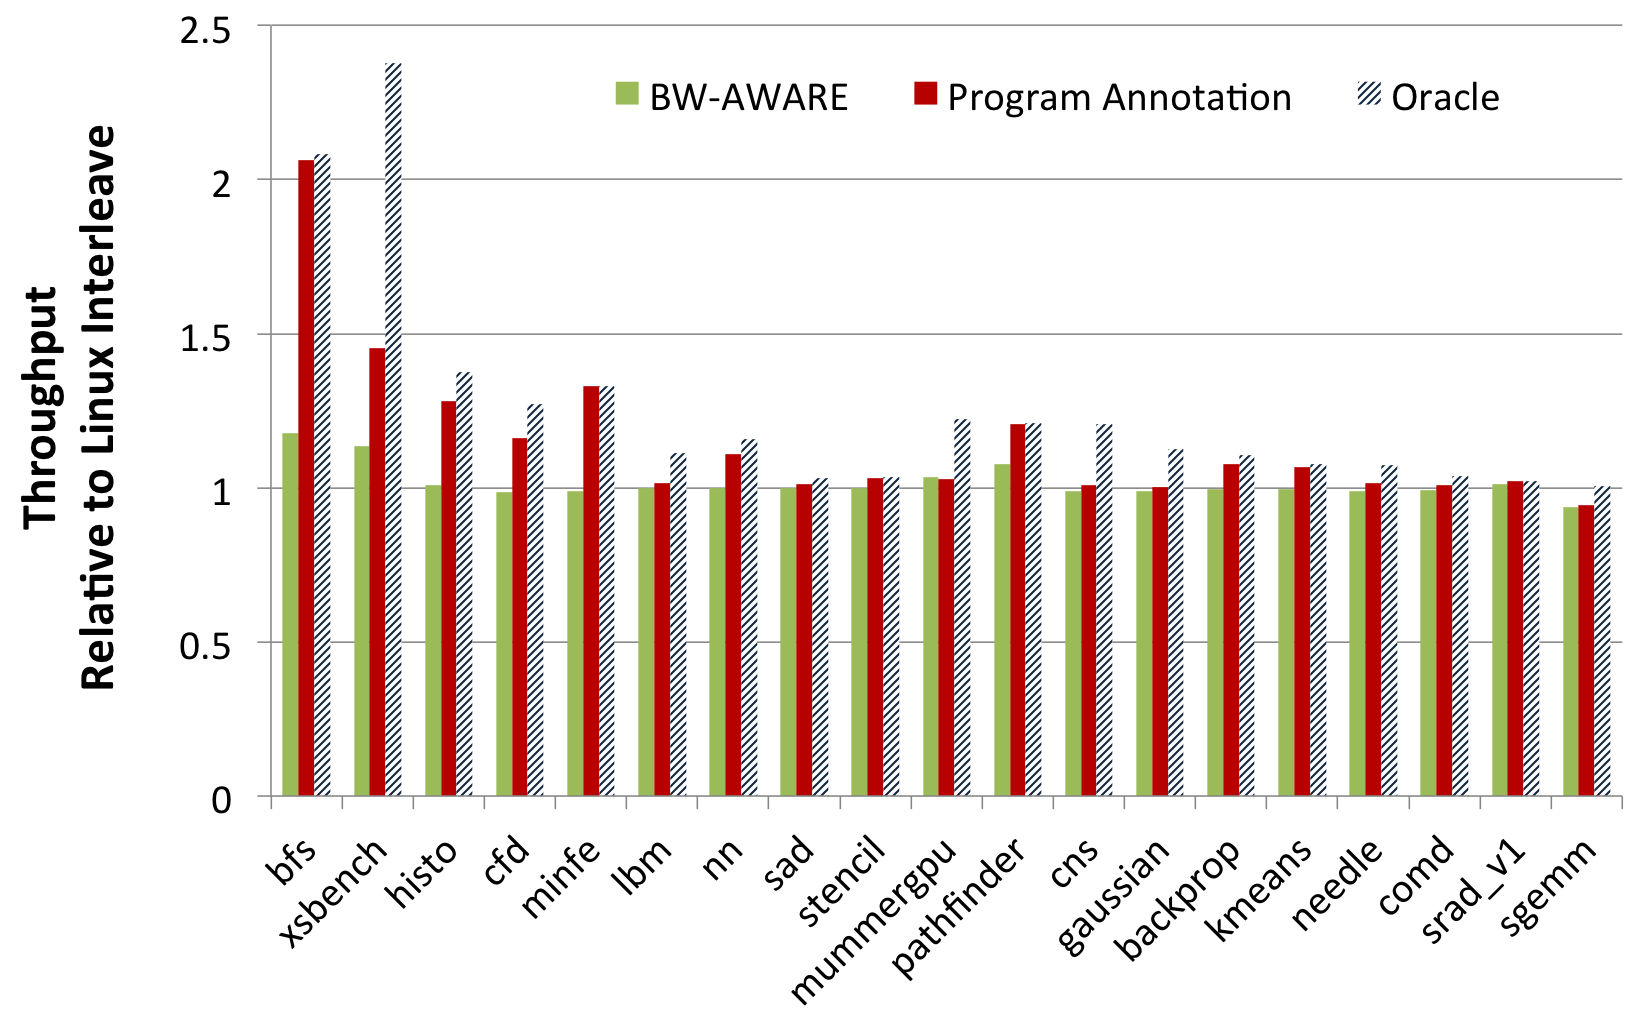
\includegraphics[width=\columnwidth]{asplos2015/figures/appannotated-10per.png}
    \caption{Profile-driven annotated page placement performance relative to INTERLEAVE, BW-AWARE and oracular policies
    under at 10\% capacity constraint.}
    \label{fig:annotated}
\end{figure}

One of the drawbacks to profile-driven optimization is that data dependent
runtime characteristics may cause different behaviors than were seen during
the profiling phase. While GPU applications in production will be run without code
modification, the data set and parameters of the workload typically vary in both
size and value from run-to-run.
Figure~\ref{fig:sensitivitytotraining} shows the sensitivity of our workload performance to
data input set changes, where placement was trained on the first data-set but
compared to the oracle placement for each individual dataset.
We show results for the four example applications which saw the highest improvement
of oracle placement over BW-AWARE.\@ For {\tt bfs}, we varied the number 
of nodes and average degree of the graph.
For {\tt xsbench}, we changed three parameters: number of nuclides, number of
lookups, and number of gridpoints in the data set. For {\tt minife}, we varied
the dimensions of the finite element problem by changing the input matrix.
Finally, for {\tt mummergpu}, we changed the number of queries and length of
queries across different input data sets.

Using the profiled information from only the training set, we observe that annotated
placement performs 29\% better than the baseline Linux INTERLEAVE policy,
performs 16\% better than our 
own BW-AWARE 30C-70B placement, and achieves 80\% of the oracle placement performance.  This 
result indicates that for GPU compute applications, feedback-driven optimization for page placement
is not overly sensitive to application dataset or parameter variation, although pessimistic
cases can surely be constructed.


%\vspace{-0.05in}
\subsection{Discussion}
\vspace{-0.05in}
The places where annotation-based placement falls short primarily come from
three sources.  First, our application profiling relies on spatial locality of virtual addresses 
to determine page hotness.  We have shown that this spatial locality holds true
for many GPU applications, but this is not guaranteed to always be the case. Allocations within 
libraries or larger memory ranges the programmer chooses
to logically sub-allocate within the program will not exhibit this property. 
The second shortcoming of our annotation-based approach is for applications 
which show high variance within a single data structure.  {\color{black}For example, when using a hashtable 
where the application primarily accesses a small, dynamically determined portion of the total key-space,
our static hotness profiling will fail to distinguish the hot and cold regions of this structure}.  Finally,
although our runtime system abstracts the programming challenges of writing
performance portable code for heterogeneous machines, it is still complex and puts
a large onus on the programmer.  Future work will be to learn from our current
implementation and identify mechanisms to reduce the complexity we expose to the programmer
while still making near-ideal page placement decisions.

\begin{figure}[t]
    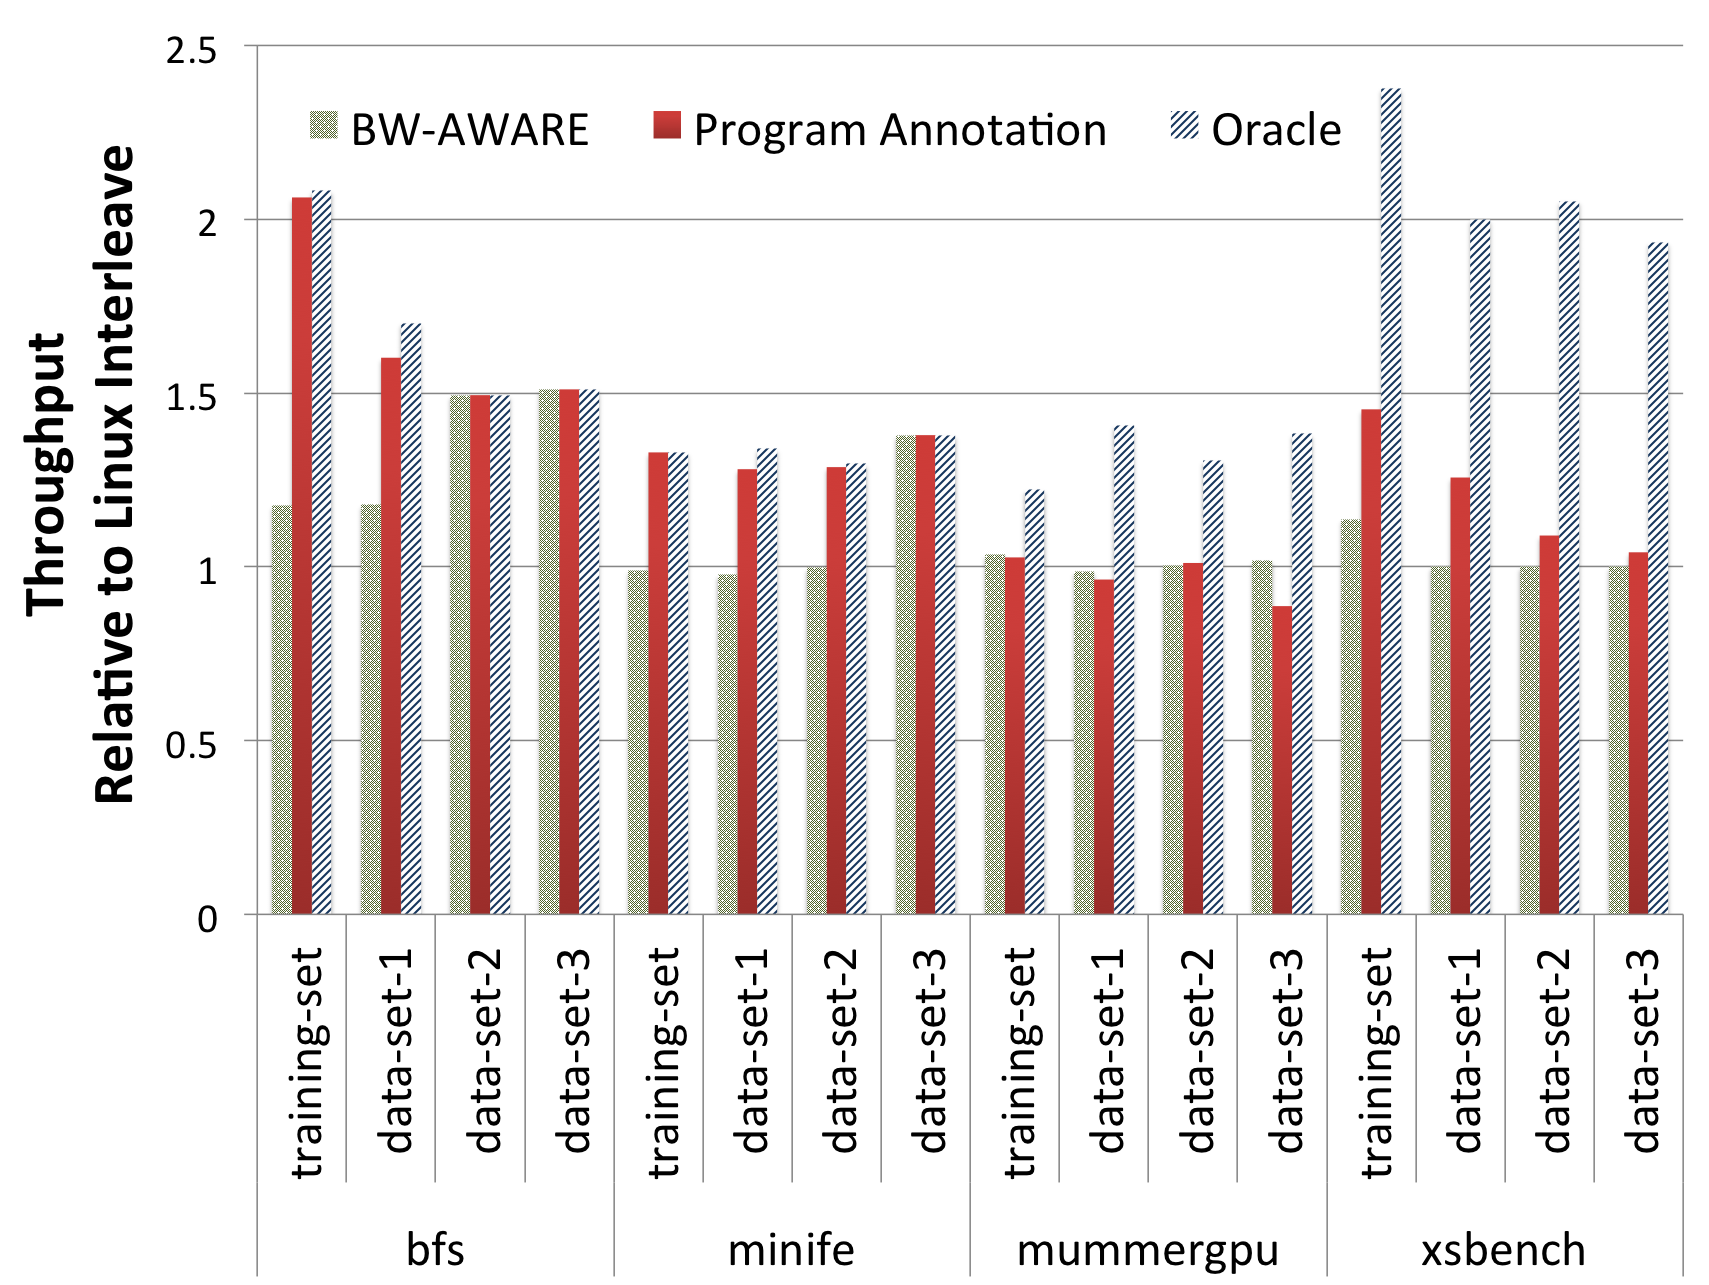
\includegraphics[width=\columnwidth]{asplos2015/figures/sensitivitytotraining.png}
    \caption{Annotated page placement effectiveness versus data sets variation after training phase under at 10\% capacity constraint.}
    \label{fig:sensitivitytotraining}
\end{figure}

In this work we have focused on page placement for applications assuming a static
placement of pages throughout the application runtime. We recognize that temporal phasing in
applications may allow further performance improvement but have chosen to focus
on initial page placement rather than page migration for two reasons.  First,
software-based page migration is a very expensive operation.  Our measurements on the Linux 3.16-rc4 
kernel indicate that it is not possible to migrate pages between NUMA memory zones at a rate faster
than several GB/s and with several microseconds of latency between invalidation and first
re-use.  While GPUs can cover several hundred nanoseconds of memory latency, microsecond
latencies encountered during migration will induce high overhead stalls within the compute pipeline.
Second, online page migration occurs only after some initial placement decisions have been
made.  Focusing on online page migration before finding an optimized initial placement policy
is putting the cart before of the horse.  With improved default page placement
for GPU workloads, the need for dynamic page migration is reduced.  Further work is needed 
to determine if there is significant value to justify the expense of online profiling 
and page-migration for GPUs beyond improved initial page allocation.

%\vspace{-0.05in}
\section{Conclusions}
%\vspace{-0.05in}
\label{conclusions}

Current OS page placement policies are optimized for both homogeneous memory and
latency sensitive systems.  We propose a new BW-AWARE page placement policy that
uses memory system information about heterogeneous memory system characteristics to place data
appropriately, achieving 35\% performance improvement on average over existing
policies without requiring any application awareness.  In future CC-NUMA
systems,
BW-AWARE placement improves the performance optimal capacity by better using
all system resources. But some applications may wish to size their problems
based on total capacity rather than performance. In such cases, we provide insight into
how to optimize data placement by using the CDF of the application in
combination with application annotations enabling intelligent runtime
controlled page placement decisions.  We propose a profile-driven application
annotation scheme that enables improved placement without requiring any
runtime page migration. While only the beginning of a fully automated
optimization system for memory placement, we believe that the performance gap between the current
best OS INTERLEAVE policy and the annotated performance (min 1\%, avg 20\%, max
2x) is enough that further work in this area is warranted as mobile, desktop,
and HPC memory systems all move towards mixed CPU-GPU CC-NUMA heterogeneous memory systems.



 \chapter{Unlocking Bandwidth for GPUs in CC-NUMA Systems}
 \label{chap:hpca2015}
 %\begin{abstract}
The advent of denser/cheaper memory technologies has renewed interest in
two-tiered main memory schemes, where cold data are shifted to slow memory to
enable greater capacity or reduce cost.  Past research on two-tiered main memory
has assumed a 4KB page size.  However, our recent work demonstrates that 2MB
(transparent) huge pages are performance critical in Cloud applications.  We
propose to develop a transparent huge-page-aware two-tiered memory solution,
targeting virtualized cloud applications, which integrates support for dynamic
page migration and transparent huge pages, achieving both the capacity/cost
advantages of two-tiered memory and performance advantages of huge pages. Hot
regions within otherwise cold huge pages present a central challenge to our
objective. We propose translation facades, a 4KB translation that remaps a
portion of a 2MB mapping with an alternate physical address or permissions, to
facilitate remapping hot portions of cold huge pages.
\end{abstract}

%\vspace{-0.05in}
\section{Introduction}
%\vspace{-0.05in}
%GPUs have enabled parallel processing for not just graphics applications but
%for a wide range of HPC installations and data-centers like Amazon's elastic
%compute cloud (EC2).  With this massively parallel processing often comes an
%insatiable demand for main memory bandwidth as GPUs churn through data at an
%ever increasing rate.  To meet this bandwidth demand, many GPUs have been
%designed with attached high-bandwidth GDDR memory rather than standard DDR
%memory used by CPUs.  As a result, many GPUs today have GDDR bandwidth that is
%2-5$\times$ higher than the memory bandwidth available to the CPU in the
%system.  To make best use of the bandwidth available to GPU programs
%programmers manually copy the data over the relatively slow PCIe bus to the GPU
%memory, and -- only then -- launch their GPU kernels.  This up-front data
%allocation and transfer has been necessary since transferring data over the
%PCIe bus is a high overhead operation, and a bulk transfer of data amortizes
%this overhead. This data manipulation overhead also results in significant
%porting challenges when retargeting existing applications to GPUs, particularly
%for high-level languages that make use of libraries and dynamic memory
%allocation during application execution.
%
%\begin{figure}[t]
%    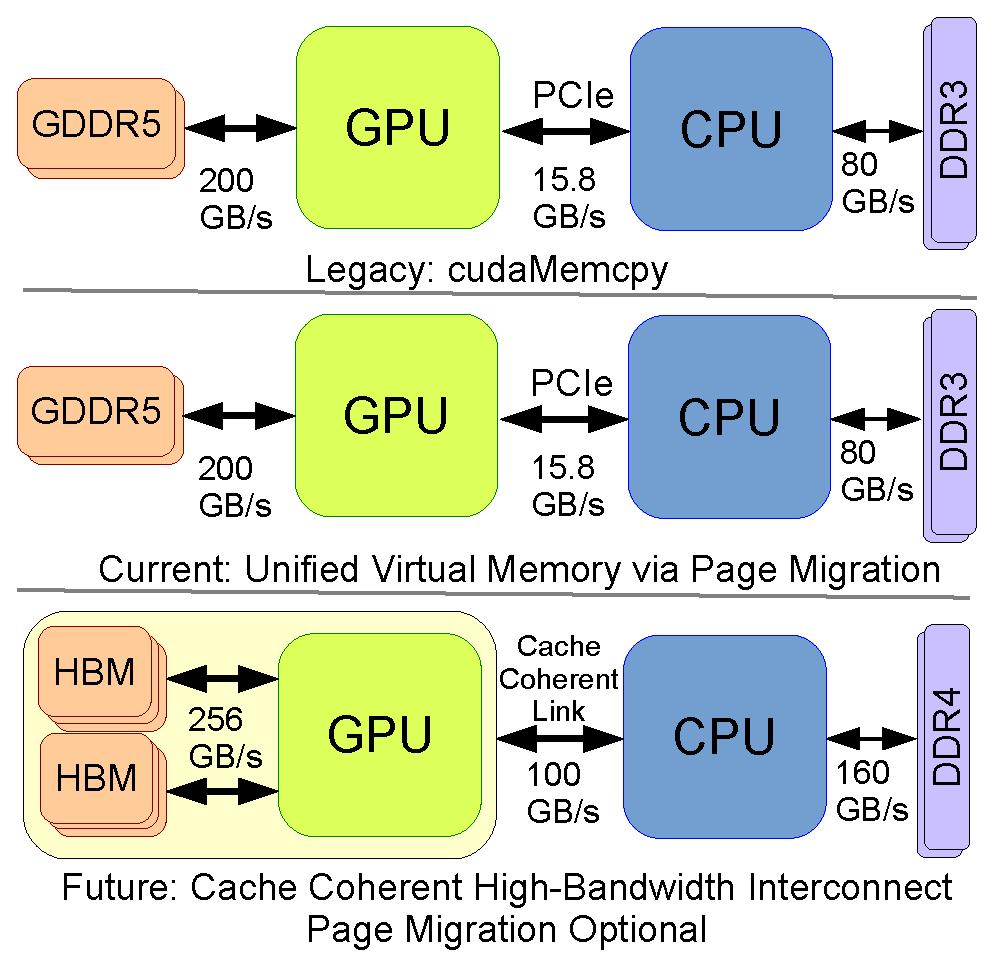
\includegraphics[width=\columnwidth]{hpca2015/figures/architecture.eps}
%    \caption{System architectures for legacy, current, and future mixed GPU-CPU systems.}
%    \label{fig:arch}
%\end{figure}
%
%Recognizing the obstacle this programming model poses to the wider adoption of
%GPUs in more parallel applications, programming systems like NVIDIA's CUDA,
%OpenCL, and OpenACC are evolving. Concurrently, GPU-CPU architectures are
%evolving to have unified globally addressable memory systems in which both the
%GPU and CPU can access any portion of memory at any time, regardless of its
%physical location.  Today this unified view of memory is layered on top of
%legacy hardware designs by implementing software-based runtimes that
%dynamically copy data on demand between the GPU and CPU~\cite{cuda}. As
%depicted in Figure~\ref{fig:arch}, over the next several years it is expected
%that GPU and CPU systems will move away from the PCIe interface to a fully
%cache coherent (CC) interface ~\cite{AMDHSA}. These systems will provide high
%bandwidth and low latency between the non-uniform memory access (NUMA) pools
%attached to discrete processors by layering coherence protocols on top of
%physical link technologies such as NVLink~\cite{NVLINK},
%Hypertransport~\cite{AMDHT}, or QPI~\cite{INTELQPI}.   CC-NUMA access to host
%memory from the GPU makes the software page migration used today an optional
%feature thanks to the improved bandwidth, latency, and access granularity that
%cache coherence can provides.
%
GPUs are throughput oriented processors that spawn thousands of threads
concurrently, demanding high memory bandwidth. To maximize the bandwidth
utilization programmers copy over the data to high bandwidth memory like GDDR5
before launching GPU kernels to amortize the overhead of accessing memory over
microsecond link latencies like PCIe. Hence, it is the responsibility of the
programmer to identify data that will be accessed by the GPU and copy it over to
the GPU-attached high bandwidth memory. NVIDIA's unified virtual
memory~\cite{UVM} has relaxed this constraint to enhance GPU programmability by
providing a software mechanism that performs on demand {\tt memcpy} of the data
as GPU accesses it. However, on demand data copying hurts GPU throughput. In
this chapter we discuss techniques of performing programmer agnostic dynamic
memory migration of performance critical data across CC-NUMA CPU-GPU system
connected by a next generation interconnect technology to maximize bandwidth
utilization, while not demanding the programmer to perform explicity {\tt
memcpy(s)}.  We specifically examine how to best balance accesses through
cache-coherence and page migration.

%The contributions of this work are the following:

%While interconnect advancements improve GPU-CPU connectivity, no reduction is
%expected in the memory bandwidth differential between CPU and GPU-attached
%memory.  On-package memories such as High Bandwidth Memory (HBM) or Wide-IO2
%(WIO2) may in fact increase this differential as GPU bandwidth requirement
%continues to grow, feeding the ever increasing number of parallel cores
%available on GPUs used by both graphics and compute workloads. On the other
%hand, architects will likely continue to balance latency, power, and cost
%constraints against raw bandwidth improvement for CPU attached memory, where
%bandwidth and application performance are less strongly correlated. With
%application data residing primarily in CPU memory on application start-up, the
%GPU can access this memory either via hardware cache-coherence (which improves
%memory system transparency to the programmer) or by migrating a memory page into
%GPU physical memory (facilitating greater peak bandwidth for future requests).
%In this work we specifically examine how to best balance accesses through
%cache-coherence and page migration for a hypothetical CC-NUMA GPU-CPU system
%connected by a next generation interconnect technology.  The contributions of
%this work are the following:

%\begin{enumerate}
%\item
%1) Counter-based metrics to determine when to migrate pages from the CPU to GPU 
%are insufficient for finding an optimal migration policy to exploit GPU memory bandwidth. 
%In streaming workloads, where each page
%may be accessed only a few times, waiting for $N$ accesses to occur before
%migrating a page will actually limit the number of accesses that occur after
%migration, reducing the efficacy of the page migration operation.

%\item
%2) TLB shootdown and refill overhead can significantly degrade the
%performance of any page migration policy for GPUs\@. We show that combining reactive
%migration with virtual address locality information to aggressively prefetch pages
%can mitigate much of this overhead, resulting in increased GPU throughput.

%\item
%3) The legacy intuition to migrate all data to the GPU local memory in an attempt to maximize bandwidth fails to leverage
%the bandwidth available via the new CC-NUMA interface.  A page migration policy which 
%is aware of this differential and balances migration with CC-NUMA link
%utilization will outperform either GPU or GPU memory being used in isolation.

%\item 
%4) We present a software based memory placement system that, on average, outperforms CC-NUMA based
%accesses by 1.95$\times$, performs 6\% better than the legacy CPU to GPU {\tt
%memcpy} approach by 
%intelligently using both CPU and GPU memory bandwidth, and comes within 28\% of oracular page placement,
%all while maintaining the relaxed memory semantics of modern GPUs.
%\end{enumerate}

%\vspace{-0.05in}
\section{Motivation and Background}
\label{background}
\vspace{-0.05in}

\begin{figure}[t]
        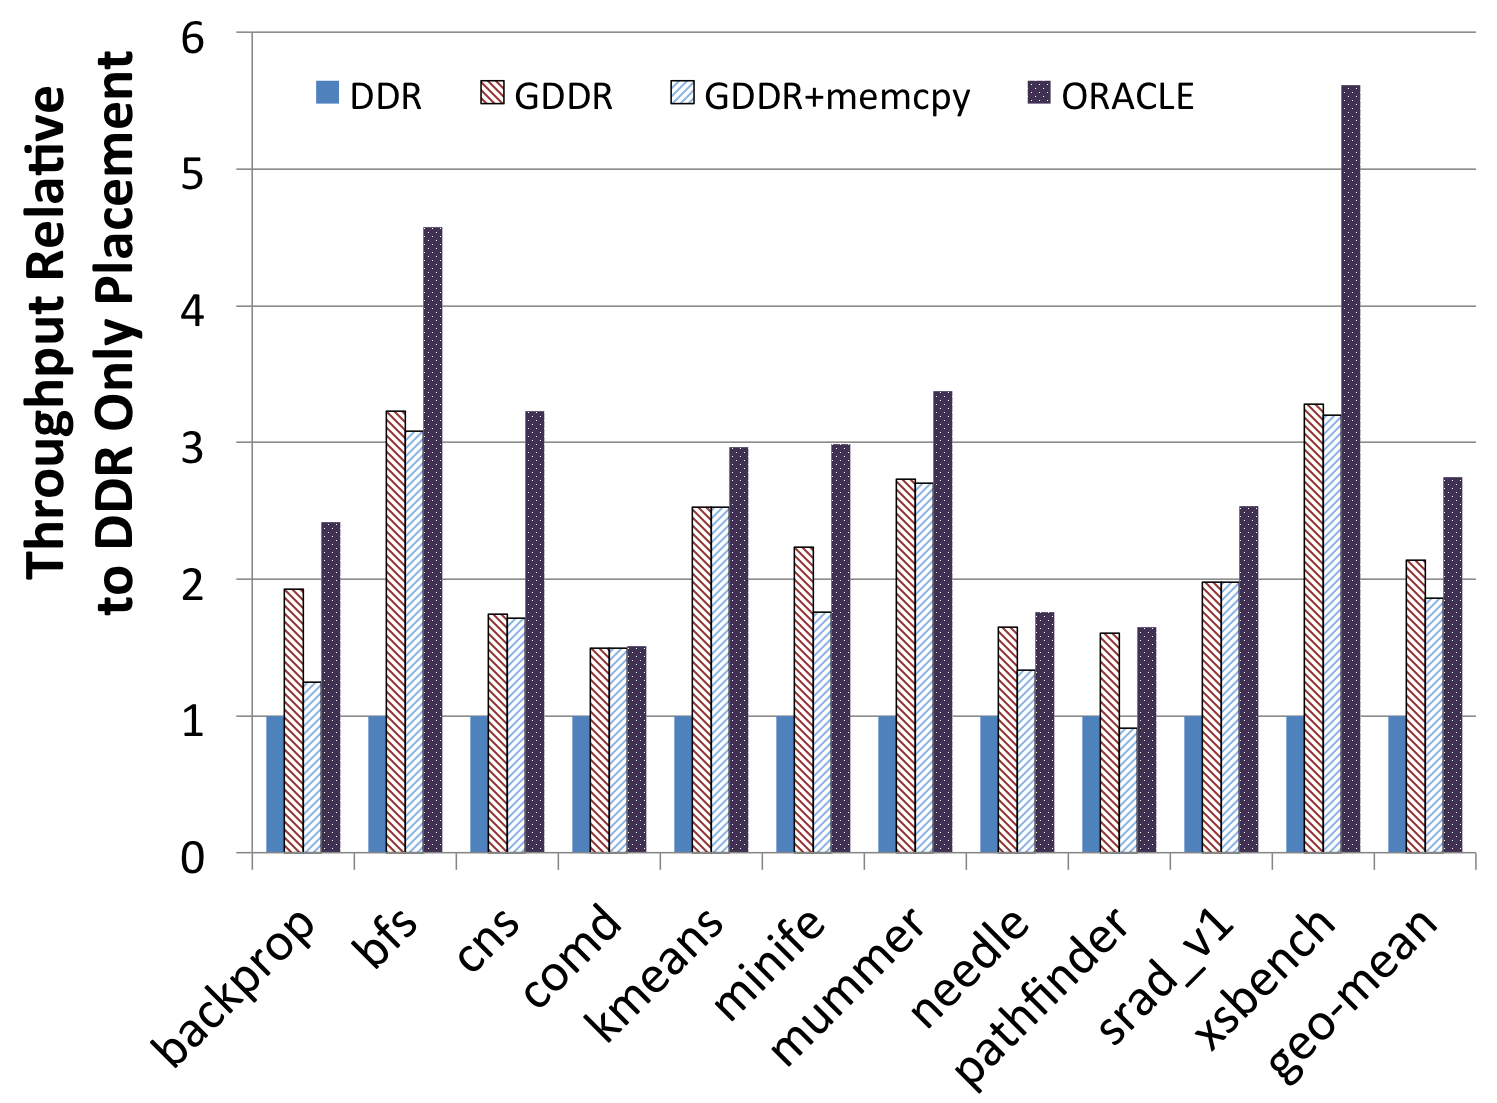
\includegraphics[width=\columnwidth]{hpca2015/figures/motivation.png}
    \caption{GPU performance sensitivity to memory subsystem performance where GDDR provides 
    200GB/s, DDR provides 80GB/s, and {\tt memcpy} bandwidth is 80GB/s.}
    \label{fig:motivation}
\end{figure}

A by-product of the GPU's many-threaded design is that
it is able to maintain a large number of in-flight memory requests and execution throughput
is correlated to memory bandwidth rather than latency, as compared to CPU designs.  As a result,
GPUs have chosen to integrate high bandwidth off-package memory like GDDR rather than accessing
the CPU's DDR directly or integrating DDR locally on the GPU board.  This choice is motivated
by our observation that the performance of some GPU compute workloads would degrade by as much as 
66\% if the traditional GDDR memory on a GPU were replaced with standard DDR memory, as seen in 
Figure~\ref{fig:motivation}.

In current CPU/GPU designs, GPU and CPU memory systems are private and require
explicit copying to the GPU before the application can execute.   Figure~\ref{fig:motivation}
shows the effect of this copy overhead on application performance by comparing GDDR to GDDR+{\tt memcpy}
performance which includes the cost of the programmer manually copying data from the DDR to the GDDR
before launching the GPU kernels.  While this copy overhead varies from application to application,
it can be a non-trivial performance overhead for short-running GPU applications and can even negate the 
effectiveness of using the high bandwidth GDDR on-board the GPU in a limited number of cases.

While it is technically possible for the GPU to access CPU memory directly over PCIe today, the long
latency (microseconds) of the access makes this a rarely used memory operation. 
Programming system
advancements enabling a uniform global address space, like those introduced in
CUDA 6.0~\cite{cuda}, relax the
requirement forcing programmers to allocate and explicitly copy memory to the GPU up-front, but
do nothing to improve the overhead of this data transfer. Further, by copying pages from the CPU to the GPU 
piece-meal on demand, these new runtimes often introduce additional overhead compared to
performing a highly optimized bulk transfer of all the data that the GPU will need during execution.
The next step in the evolution of GPUs, given the unified addressing, is
to optimize the performance of this new programming model. 

\subsection {Cache Coherent GPUs}

The key advancement expected to enable
performance is the introduction of CC-NUMA GPU and CPU systems.  Using cache coherence layered upon NVLink, HT, or QPI, GPUs will
likely be able to access CPU memory in hundreds of nanoseconds at bandwidths up to 128GB/s by bringing
cache lines directly into GPU caches. Figure~\ref{fig:motivation} shows the upper bound (labeled ORACLE) on performance
that could be achieved if both the system DDR memory and GPU GDDR memory were used concurrently, assuming data had 
been optimally placed in both technologies.  In this work, we define oracle placement to be \emph{a priori} page placement
in the GPU memory (thus requiring no migration), of the minimum number of pages, when sorted from hottest to coldest, 
such that the GDDR bandwidth is fully subscribed during application execution.

Because initial CPU/GPU CC-NUMA systems are likely to use a form of IOMMU address translation services 
for walking the OS page tables within the GPU,  it is unlikely that GPUs will be able to directly
allocate and map their own physical memory without a call back to the CPU and operating system.
In this work, we make a baseline assumption that all physically allocated pages are initially allocated
in the CPU memory and only the operating system or GPU runtime system executing on the host can initiate
page migrations to the GPU\@.  In such a system, two clear performance goals become evident.
The first is to design a memory policy that balances CC-NUMA access and page migration to simply achieve the 
performance of the legacy bulk copy interface without the programming limitations.  The second, more ambitious, goal
is to exceed this performance and approach the oracular performance by using these memory zones concurrently, enabling 
a peak memory bandwidth that is the sum of the two zones.

Achieving either of these goals requires
migrating enough data to the GPU to exploit its high memory bandwidth while avoiding migrating pages
that may never be accessed again.  Every page migration increases the total bandwidth requirement of the
application and over-migration potentially reduces application performance if sufficient bandwidth headroom in both the DDR and GDDR is not available.
Thus, the runtime system must be selective about which pages to migrate.  The runtime system also must be cognizant
that performing TLB invalidations (an integral part of page migration) on a GPU does not just halt a single
processor, but thousands of compute pipelines that may be accessing these pages through a large shared TLB structure.
This shared TLB structure makes page migrations between a CPU and GPU potentially much more costly (in terms of the opportunity cost of lost execution throughput) than in CPU-only systems.

In addition to managing the memory bandwidth overhead
of page migration and execution stalls due to TLB shootdowns, the relative bandwidth utilization of both the CPU and GPU memory 
must be taken into account when making page migration decisions.  When trying to balance memory bandwidth between two distinct memory
zones, it is possible to over- or under-subscribe either memory zone. Migrating pages too slowly to the GPU
memory will leave its local memory sitting idle, wasting precious bandwidth.  Conversely, migrating pages
to the GPU too aggressively may result in under-utilization of the CPU memory while paying the maximum cost in terms
of migration overheads. A comprehensive CPU-GPU memory management solution will attempt to balance all of 
these effects to maximize memory system and GPU throughput in future mobile, graphics, HPC, and datacenter
installations.

\subsection{Related Work}
\label{related_work}
\vspace{-0.05in}

Using mixed DRAM technologies or DRAM in conjunction with non-volatile memories
to improve power consumption on CPUs has been explored by several groups
~\cite{Kultursay2013,Phadke11mlpaware2011,Mogul2009,Bheda2011,Ramos2011}.
The majority of this work attempts to overcome the performance reductions introduced
by non-DDR technologies to improve capacity, power consumption, or both.
In CC-NUMA systems, there has been a long tradition of examining where to place
memory pages and processes for optimal performance, typically focusing on reducing
memory latency~\cite{Wilson2001,Bolosky1989,Brecht1993,LaRowe1992,Verghese1996,Iyer1998}.
Whereas CPUs are highly sensitive to memory latency, GPUs can cover a much larger latency
through the use of multi-threading.  More recent work on page placement and 
migration~\cite{AUTONUMA,Dashti2013,Tam2007,Zhuravlev2010,Knauerhase2008,Blagodurov2011,awasthinellans10}
has considered data sharing characteristics, interconnect utilization, and memory controller
queuing delays in the context of CPU page placement. However, the primary improvements in many of these works,
reducing average memory latency, will not directly apply in a GPU optimized memory system.

Several recent papers have explored hybrid DRAM-NVM GPU attached memory subsystems~\cite{zhao2013,Wang2013}.
Both of these works consider a traditional GPU model where the availability of low latency, high bandwidth access to CPU-attached 
memory is not considered, nor are the overheads of moving data from the host CPU onto the GPU considered.
Several papers propose using a limited capacity, high bandwidth memory as a
cache for a larger slower memory~\cite{jiang2011,Meza2012}, but such designs incur a high engineering
overhead and would require close collaboration between GPU and CPU vendors that often do not
have identically aligned visions of future computing systems.

When designing page migration policies, the impact of TLB shootdown overheads and page table updates is a constant
issue.  Though most details about GPU TLBs are not public,
several recent papers have provided proposals about how to efficiently implement general purpose TLBs
that are, or could be, optimized for a GPU's needs~\cite{Pichai2014,Villavieja2011,Power2014}. Others
have recently looked at improving TLB reach by exploiting locality within the virtual to physical
memory remapping, or avoiding this layer completely~\cite{swansonstoller98,Pham2014,Basu2013}.  
Finally, Gerofi et al.~\cite{Gerofi2014} recently examined TLB performance of the Xeon Phi
for applications with large footprints, while McCurdy et al.~\cite{McCurdy2008} investigated the
effect of superpages and TLB coverage for HPC applications in the context of CPUs.

\begin{figure}[t]
    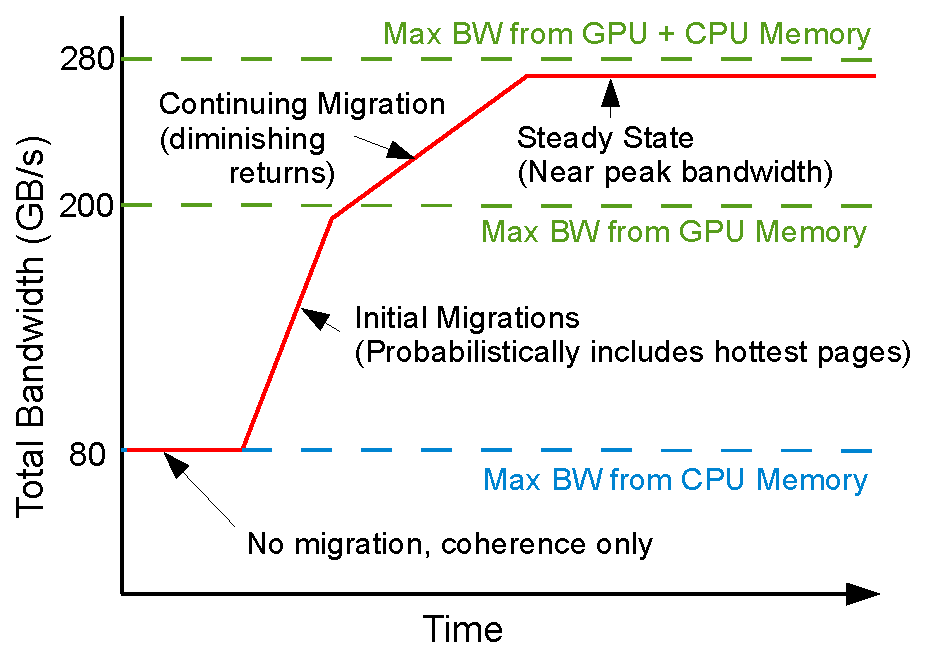
\includegraphics[width=\columnwidth]{hpca2015/figures/opportunity.eps} 
    \caption{Opportunity cost of relying on cache coherence versus migrating pages near beginning of application run.}
    \label{fig:opportunity}
\end{figure}

\vspace{-0.05in}
\section{Balancing Page Migration and Cache-Coherent Access}
\label{threshold}

In the future, it is likely GPUs and CPUs will use a shared page table structure
while maintaining local TLB caches.  It remains to be seen if the GPU will be
able to natively walk the operating system page tables to translate virtual to
physical address information, or if GPUs will use an IOMMU-like hardware in
front of the GPU's native TLB to perform such translations.  In either case, the
translation from virtual to physical addresses will be implicit, just as it is
today for CPUs, and will no longer require trapping back to the CPU to translate
or modify addresses.  As a result, when page mappings must be modified, all
CPUs---and now the GPU---must follow appropriate steps to safely invalidate
their local TLB caches.  While CPUs typically use a TLB per CPU-core, GPUs use a
multi-level global page table across all compute pipelines.  Therefore, when TLB
shootdowns occur, the penalty will not stall just a single CPU pipeline, it is
likely to stall the entire GPU\@. Whereas recent research has proposed intra-GPU
sharer tracking~\cite{Villavieja2011} that could mitigate these stalls, this
additional hardware is costly and typically unneeded for graphics applications
and thus may not be adopted in practice.

Figure~\ref{fig:opportunity} provides a visual representation of the effect of
balancing memory accesses from both DDR (CPU-attached) and GDDR (GPU-attached)
memory. Initially, pages reside entirely in DDR memory.  Without migration, the
maximum bandwidth available to GPU accesses (via cache coherence to the DDR
memory)  will be limited by either the interconnect or DDR memory bandwidth.  As
pages are migrated from DDR to GDDR, the total bandwidth available to the GPU
rises as pages can now be accessed concurrently from both memories.  Migrations
that occur early in kernel execution will have the largest effect on improving
total bandwidth, while later migrations (after a substantial fraction of GDDR
memory bandwidth is already in use) have less effect.  Performance is maximized
when accesses are split across both channels in proportion to their peak
bandwidth.  Figure~\ref{fig:opportunity} shows the total bandwidth that is
wasted if pages are not migrated eagerly, early in kernel execution.  The key
objective of the migration mechanism is to migrate the hottest pages as early as
possible to quickly ramp up use of GDDR memory bandwidth.  Nevertheless,
migrating pages that are subsequently never accessed wastes bandwidth on both
memory interfaces.  In this section, we investigate alternative DDR-to-GDDR
memory migration strategies.  In particular, we contrast a simple, eager
migration strategy against more selective strategies that try to target only hot
pages.

\subsection{Methodology}
To evaluate page migration strategies, we model a GPU with a heterogeneous
memory system comprising both  GDDR and DDR memories. We discuss our baseline
simulation framework in Chapter~\ref{chap:asplos2015:baseline-methodology}.
%The GDDR memory is directly attached and addressable by the GPU, as in existing
%systems.  We assume DDR memory may be accessed by the GPU via a
%cache-line-granularity coherent interface at an additional 100 GPU cycle
%latency (in addition to the DDR access latency).  We derive our latency
%estimates from SMP CPU interconnects~\cite{INTELXEON}.  We find that these
%additional 100 cycles of latency have relatively little impact on GPU
%application performance (compared to a hypothetical baseline with no additional
%latency), as GPUs are already effective in hiding such latency.  Across the
%suite of applications we study, the mean performance degradation due to
%interconnect latency is 3\%, and at worst 10\%.
%
%We extend GPGPU-Sim~\cite{gpgpusim_ispass09} with a model of this GDDR5-DDR4
%heterogeneous memory.
Table~\ref{tab:asplos2015:bw-methodology} lists memory configuration of our simulation
framework.
%We make several additional enhancements to the baseline GTX-480 model to better
%match the bandwidth requirements of future GPUs (e.g., increasing the number of
%miss status handling registers, increasing clock frequency, etc).  We assume a
%GDDR bandwidth of 200GB/s and a DDR bandwidth of 80 GB/s.

%\begin{table}[t]
%\begin{center}
%\begin{tabular}{|l|l|}
%%\hline
%%Simulator & GPGPU-Sim 3.x\\
%%\hline
%%GPU Arch & NVIDIA GTX-480 Fermi-like\\
%%\hline
%%GPU Cores& 15 {\color{black}SMs} @ 1.4Ghz\\
%%\hline
%%L1 Caches & 16kB/SM \\
%%\hline
%%L2 Caches & Memory Side 128kB/DRAM Channel\\
%%\hline
%%L2 MSHRs & 128 Entries/L2 Slice\\
%%\hline
%\hline
%\multicolumn{2}{|c|}{Memory system}\\
%\hline
%GPU-Local GDDR5 & 8-channels, 200GB/sec aggregate\\
%\hline
%GPU-Remote DDR4& 4-channels, 80GB/sec aggregate\\
%\hline
%DRAM Timings & \multicolumn{1}{|l|}{RCD=RP=12,RC=40,CL=WR=12}\\
%\hline
%GPU-CPU &  100 GPU core cycles\\
%Interconnect Latency & \\
%\hline
%\end{tabular}
%\caption{Memory system configuration for heterogeneous CPU-GPU system.}
%\label{tab:mig-methodology}
%\end{center}
%\end{table}

We model a software page migration mechanism in which migrations are performed
by the CPU based on hints provided asynchronously by the GPU\@.  The GPU tracks
candidate migration addresses by maintaining a ring buffer of virtual addresses
that miss in the GPU TLB.  The runtime process on the CPU polls this ring
buffer, converts the address to the page aligned base address and initiates
migration using the standard Linux {\tt move\_pages} system call.

As in a CPU, the GPU TLB must be updated to reflect the virtual address changes
that result from migrations.  We assume a conventional x86-like TLB shootdown
model where the entire GPU is treated like a single CPU using traditional
inter-processor interrupt shootdown.  In future systems, an IOMMU performing
address translations on behalf of the GPU cores is likely to hide the specific
implementation details of how it chooses to track which GPU pipelines must be
stalled and flushed during any given TLB shootdown.  For this work, we make a
pessimistic assumption that, upon shootdown, all execution pipelines on the GPU
must be flushed before the IOMMU handling the shootdown on behalf of the GPU can
acknowledge the operation as complete. We model the time required to invalidate
and refill the TLB entry on the GPU as a parameterized, fixed number, of cycles
per page migration. In Section~\ref{thresholdresults} we examine the effect of
this invalidate/refill overhead on the performance of our migration policy,
recognizing that the implementation of TLB structures for GPUs is an active area
of research~\cite{Pichai2014,Power2014}.

We model the memory traffic due to page migrations without any special
prioritization within the memory controller and rely on the software runtime to
rate-limit our migration bandwidth by issuing no more than 4 concurrent page
migrations.  We study our proposed designs using memory intensive workloads from
Rodinia~\cite{Che2009} and some other recent HPC
applications~\cite{comd,cns,minife,xsbench}. These benchmarks cover varied
application domains, including graph-traversal, data-mining, kinematics, image
processing, unstructured grid, fluid dynamics and Monte-Carlo transport
mechanisms.

\subsection{Results}
\label{thresholdresults}
{\color{black}To understand the appropriate balance of migrating pages early (as soon as first touch on the GPU) or later (when partial information about page hotness is known),
we implemented a page migration policy in which pages become candidates for software controlled page migration only after they are touched
$N$ times by the GPU\@. Strictly migrating pages on-demand before servicing the memory requests will put 
page migration on the critical path for memory load latency. However, migrating a page after
$N$ references reduces the number of accesses that can be serviced from the GPU local memory, decreasing the potential
impact of page migration.} Once a page crosses the threshold for migration, we place it in an unbounded FIFO queue for migration, and allow
the CUDA software runtime to migrate the pages by polling this FIFO and migrating pages as described
in the previous sub-section.  

To isolate the effect of choosing a threshold value from TLB shootdown costs, we optimistically assume a TLB shootdown 
and refill overhead of 0 cycles for the results shown in Figure~\ref{fig:threshold}. This figure shows application
performance when migrating pages only after they have been touched $N$ times,
represented as threshold-$N$ in the figure.   The baseline
performance of 1.0 reflects application performance if the GPU only accesses the CPU's DDR via hardware cache coherence and no page migrations
to GDDR occur.  Although we anticipated using a moderately high threshold (64--128) would generate the best performance
(by achieving some level of differentiation between hot and cold data), the results in the figure indicate that, for the majority of the benchmarks, using the lowest threshold 
typically generates the best performance.  Nevertheless, behavior and sensitivity to the threshold varies significantly across applications.

\begin{figure}[t]
    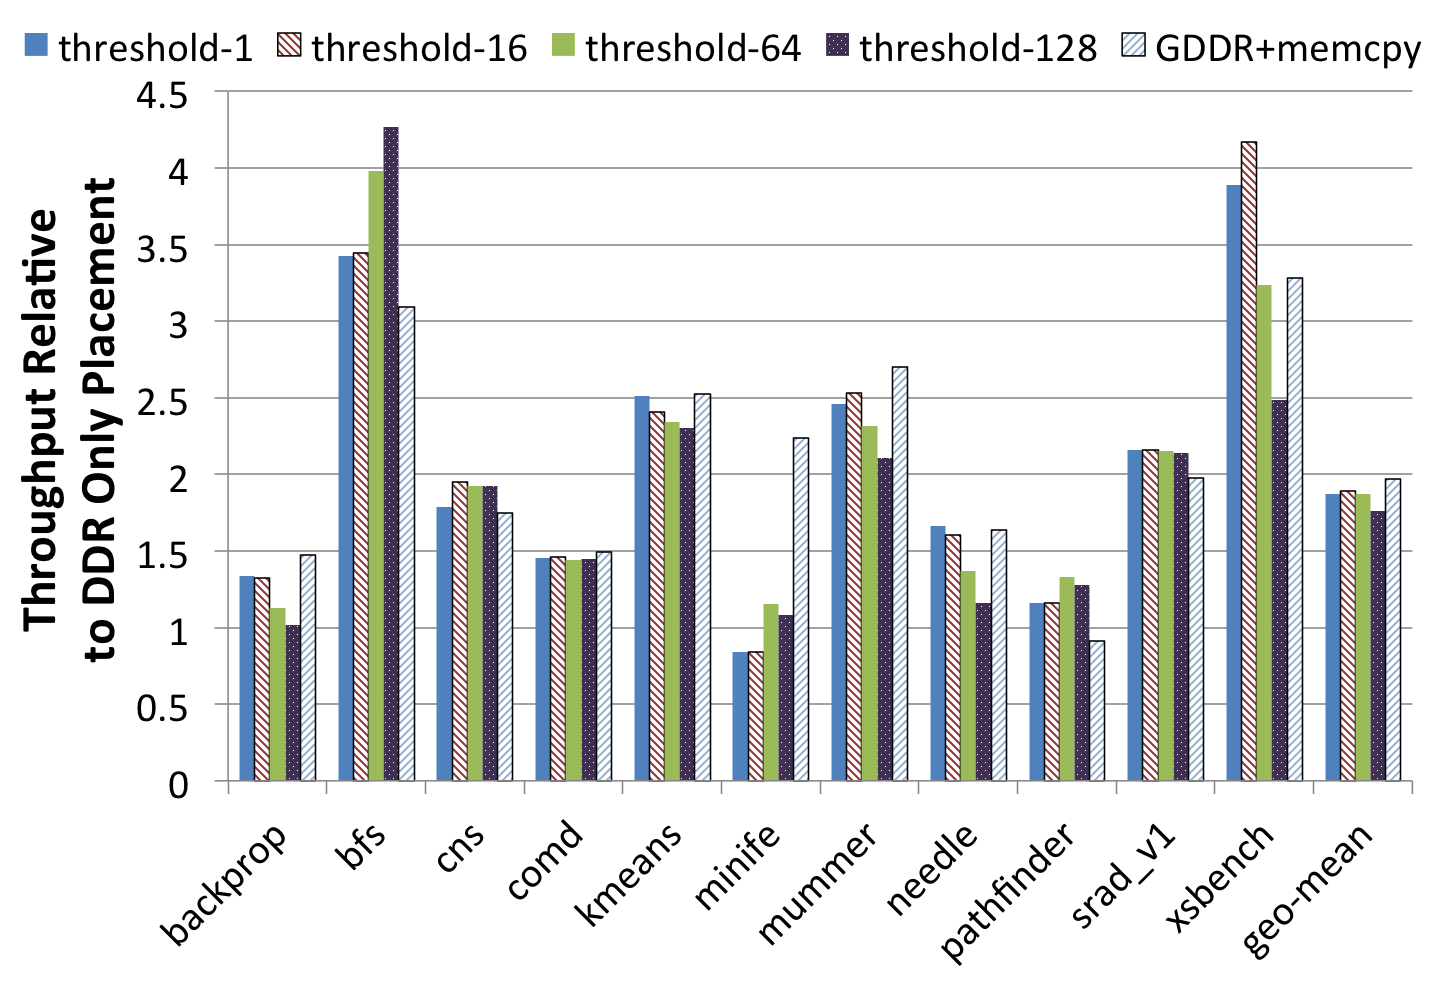
\includegraphics[width=\columnwidth]{hpca2015/figures/staticthreshold.png} 
    \caption{Performance of applications across varying migration thresholds, where threshold-N is the number of touches a given page must receive
    before being migrated from CPU-local to GPU-local memory.}
    \label{fig:threshold}
\end{figure}

For the majority of our workloads, the best performance comes at a low migration threshold
with performance degrading as the threshold increases.  The peak performance is well above that achievable with 
only cache-coherent access to DDR memory, but it rarely exceeds the the
performance of the legacy {\tt memcpy} programming
practice. The {\tt bfs} benchmark is a notable outlier, with higher migration thresholds improving performance by successfully differentiating hot
and cold pages as candidates for migration.  However, performance variation due to
optimal threshold selection is much smaller than the substantial performance gain of using any migration policy.  {\tt Minife}
is the second substantial outlier, with a low migration threshold decreasing performance below that of using CPU-only
memory, while migration with higher thresholds provides only modest gains over  cache-coherent access to DDR\@. Further analysis revealed 
that, for this workload, migration often occurs after the application has already performed the bulk of its accesses to a given
page.  In this situation, page migration merely introduces a bandwidth tax on the memory subsystem with little possibility for
performance gain.  

To implement a threshold-based migration system in practice requires tracking the number of times a given physical page
has been touched.  Such counting potentially requires tracking all possible physical memory locations that the GPU may access
and storing this side-band information either in on-chip SRAMs at the L2, memory controller, or within the DRAM itself.  Additional
coordination of this information may be required between the structures chosen to track this page-touch information. Conversely,
a first touch policy (threshold-1) requires no tracking information and can be trivially implemented by migrating a page the first time
the GPU translates an address for the page.  Considering the performance differential
seen across thresholds, we believe the overhead of implementing the necessary hardware counters to track all pages within a system 
to differentiate their access counts is not worth the improvement over a vastly simpler first-touch migration policy.

In Figure~\ref{fig:threshold} we showed the performance improvement achievable 
when modeling the bandwidth cost of the page migration while ignoring the 
cost of the TLB shootdown, which will stall the entire GPU.  At low migration 
thresholds, the total number of pages migrated is largest and thus application 
performance is most sensitive to the overhead of the TLB shootdown and refill. 
Figure~\ref{fig:migrationoverheads} shows the sensitivity of application 
slowdown to the assumed cost of GPU TLB shootdowns for a range of client-side 
costs similar 
to those investigated by Villavieja et al.~\cite{Villavieja2011}. 
While the TLB invalidation cost in current GPUs is much higher, due to complex 
host CPU interactions, it is likely that TLB invalidation cost will drop 
substantially in the near future (due to IOMMU innovation) to a range 
competitive with contemporary CPUs (i.e., ~100 clock cycles).

Because the GPU comprises many concurrently executing pipelines, the performance 
overhead of a TLB shootdown, which may require flushing all compute pipelines, is 
high; it may stalls thousands of execution lanes rather than a single CPU core.  
Figure~\ref{fig:migrationoverheads} shows that moving from an idealized threshold of 
zero, to a realistic cost of one hundred reduces average performance by 16\%.  In 
some cases this overhead can negate the entire performance improvement achieved 
through page migration. To maximize the performance under page migration, our 
migration mechanism must optimize the trade-off between stalling the GPU on TLB 
shootdowns versus the improved memory efficiency of migrating pages to the GPU\@.  
One way to reduce this cost is to simply perform fewer page migrations, which can 
be achieved by increasing the migration threshold above the 
migrate-on-first-touch policy.  Unfortunately, a higher migration threshold also 
decreases the potential benefits of migration.  Instead, we will describe 
mechanisms that can reduce the number of required TLB invalidations simply 
through intelligent page selection while maintaining the first-touch 
migration threshold.

\begin{figure}[t]
    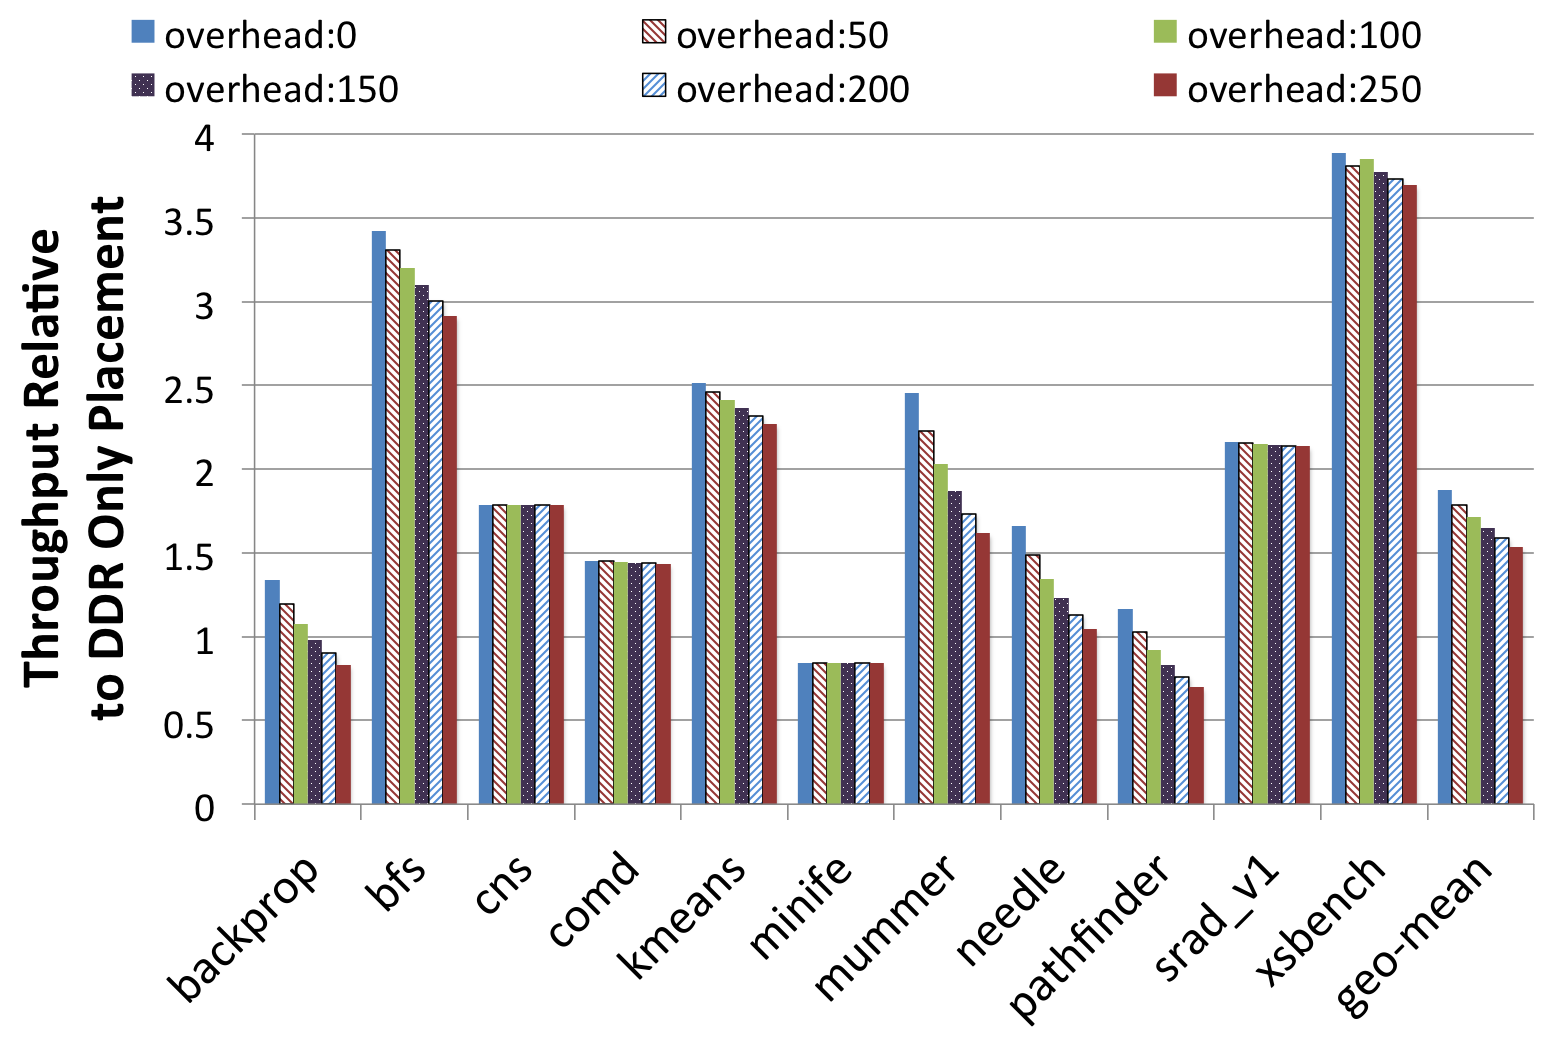
\includegraphics[width=\columnwidth]{hpca2015/figures/migrationoverheads.png} 
    \caption{Performance overhead of GPU execution stall due to TLB shootdowns when using a first touch migration policy (threshold-1).}
    \label{fig:migrationoverheads}
\end{figure}

\vspace{-0.05in}
\section{Range Expanding Migration Candidates}
\label{rangeexpansion}
\vspace{-0.05in}

In the prior section, we demonstrated that aggressively migrating pages generally improves application performance
by increasing the fraction of touches to a page serviced by higher-bandwidth (GPU-attached) GDDR versus (CPU-attached) DDR memory.  This
aggressive migration comes with high overheads in terms of TLB shootdowns and costly GPU pipeline stalls.  
One reason the legacy application directed {\tt memcpy} approach works well is that it performs both aggressive 
up-front data transfer to GDDR and does not require TLB shootdowns and stalls.  
Unfortunately, this requirement for application-directed transfer is not well suited to 
unified globally addressable memory with dynamic allocation-based programming models. 
In this section, we discuss a prefetching technique that can help regain the performance 
benefits of bulk memory copying between private memories, without the associated programming
restrictions.

Ideally, a page migration system prefetches pages into GDDR after they are allocated and populated in DDR, 
but before they are needed on the GPU\@.  Studying the results of the threshold-based migration experiments, 
we observe that pages often are migrated too late to have enough post-migration accesses to justify the 
cost of the migration.  One way to improve the timeliness of migrations is via a prefetching scheme 
we call \emph{range expansion}.   Range expansion builds on the baseline single-page migration mechanism
discussed previously. To implement basic range expansion, when the CUDA runtime is provided a virtual address to
be migrated, the runtime also schedules an additional \emph{N} pages in its (virtual address) neighborhood 
for migration.  Pages are inserted into the migration queue in the order of furthest, from the triggered address,
to the nearest, to provide the maximum prefetching affect based on spatial locality.
We then vary this range expansion amount \emph{N} from 0--128 and discuss the results in Section~\ref{rangeexpansionresults}.

The motivation for migrating (virtually) contiguous pages can be seen in
Figure~\ref{fig:cdfannotation}. The figure shows virtual page addresses that are
touched by the GPU for three applications in our benchmark set.
The X-axis shows the fraction of the application footprint when
sampled, after on-chip caches, at 4KB page granularity and sorted from
{\color{black}most to fewest accesses.
The primary Y-axis (shown figure left) shows the cumulative distribution
function of memory bandwidth among the pages allocated by the application.
Each point on the secondary scatter
plot (shown figure right) shows the virtual address of the corresponding page on
the x-axis. This data reveals that hot and cold pages are strongly clustered within the
virtual address space.  However, the physical addresses of these pages will be
non-contiguous due to address interleaving performed by the memory controller.
} This clustering
is key to range expansion because it suggests that if a page is identified for migration, then other 
neighboring pages in the virtual address space are likely to have a similar number of total touches.  
To exploit this property,
range expansion migrates neighboring virtual addresses of a migration candidate \emph{even if they
have not yet been accessed on the GPU}\@.  By migrating these pages before they are touched on the GPU, range
expansion effectively prefetches pages to the higher bandwidth memory on the GPU, 
improving the timeliness and effectiveness of page migrations.  

\begin{figure}[pth]
    \centering
    \subfloat[bfs]{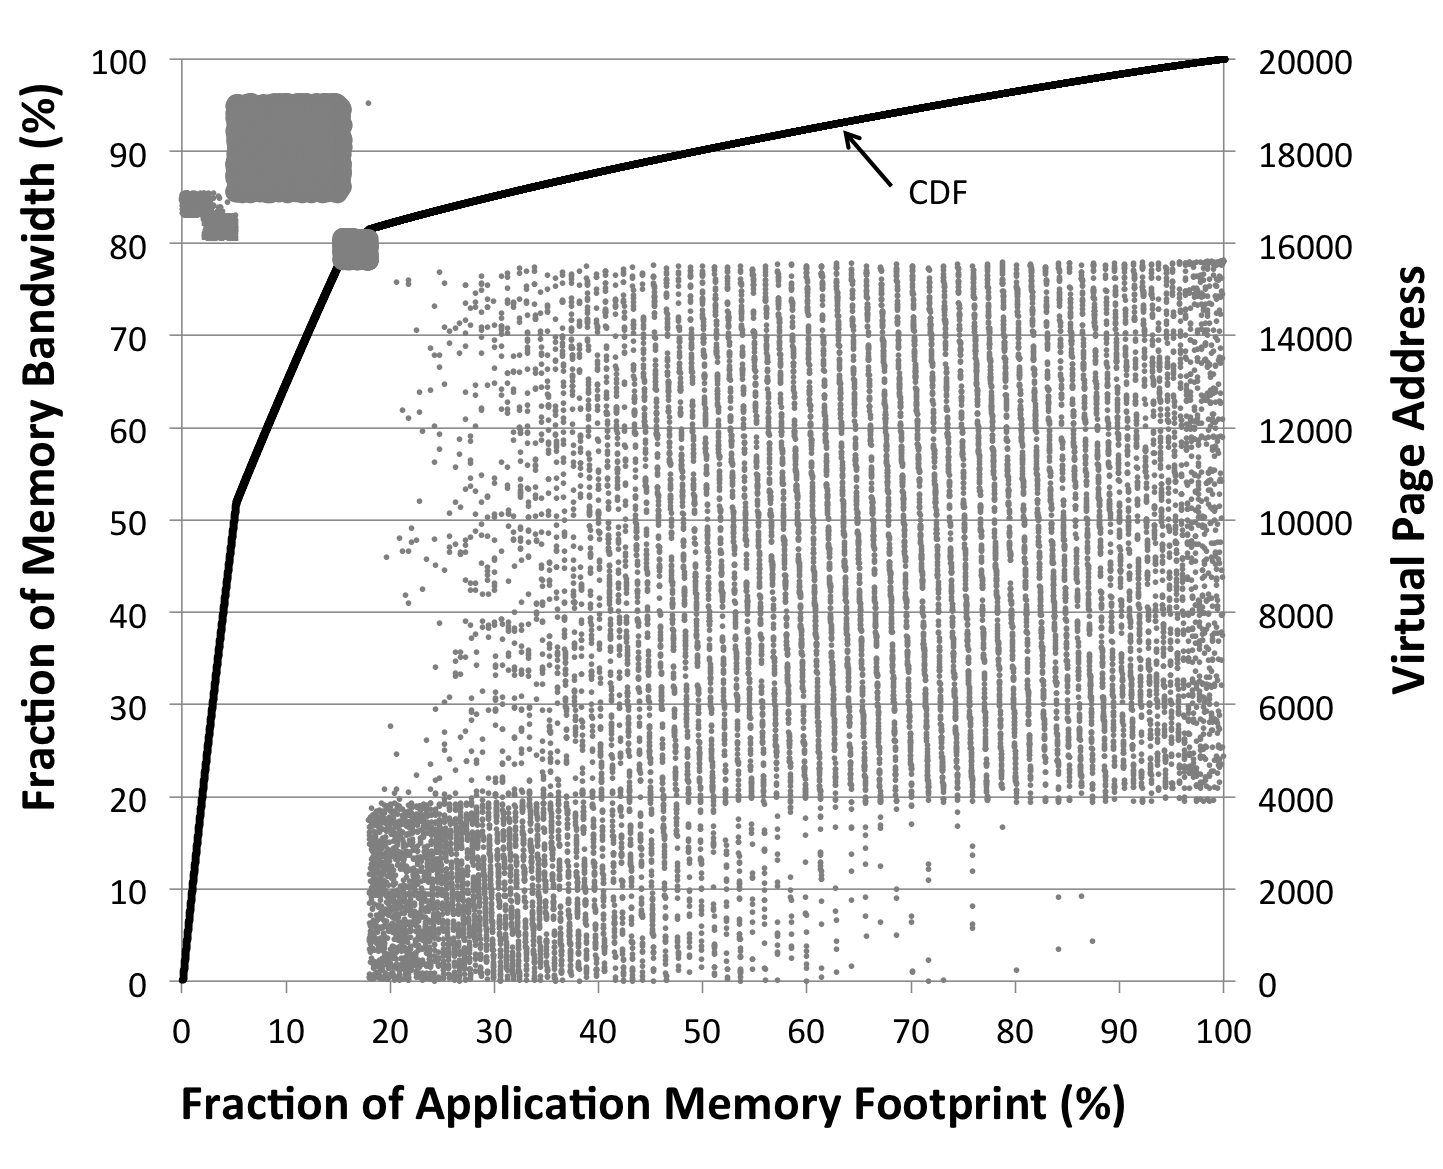
\includegraphics[width=\columnwidth]{hpca2015/figures/bfsannotated.png}}\\
    \subfloat[xsbench]{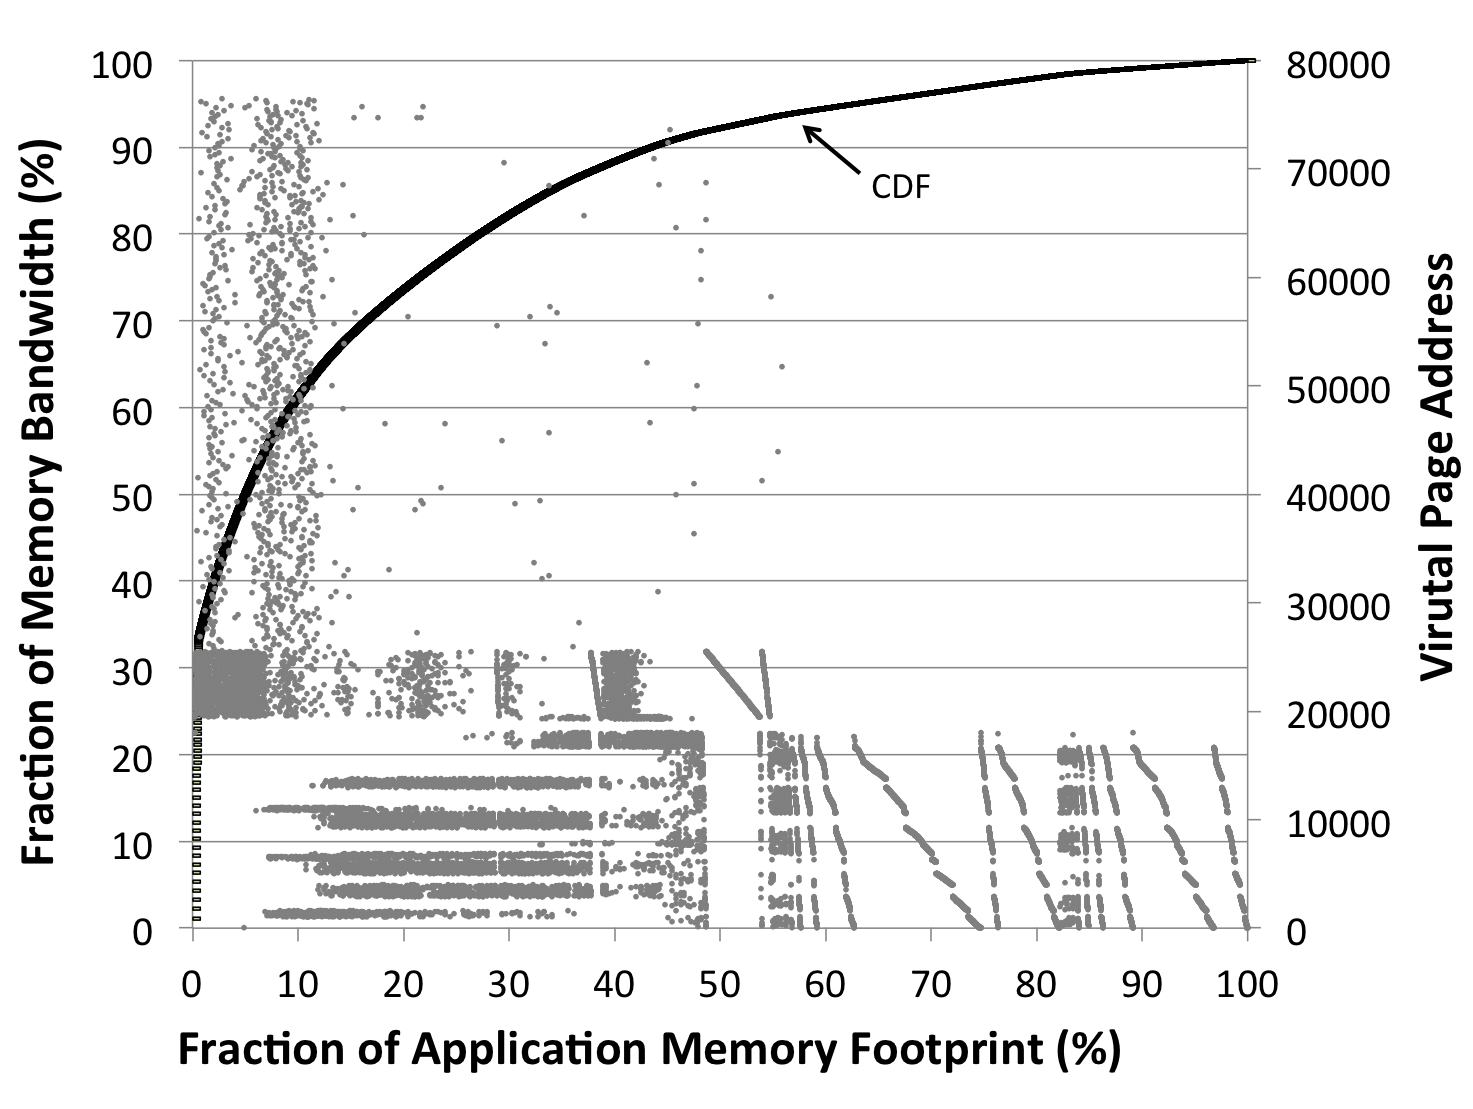
\includegraphics[width=\columnwidth]{hpca2015/figures/xsbenchannotated.png}}\\
    \subfloat[needle]{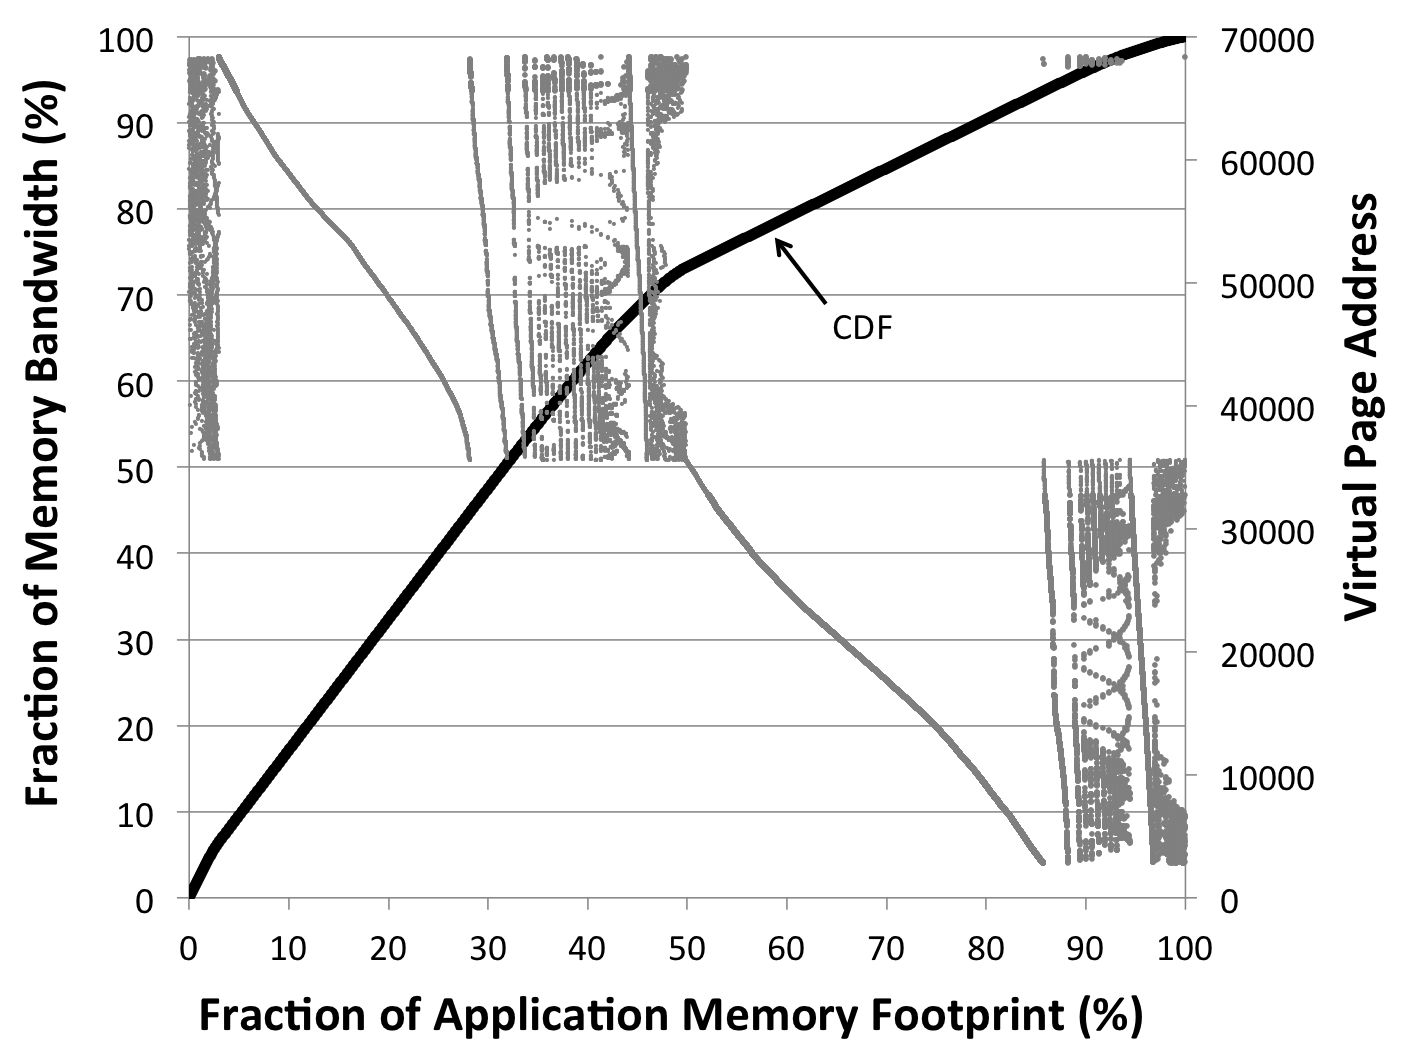
\includegraphics[width=\columnwidth]{hpca2015/figures/needleannotated.png}}\\
    \caption{Cumulative distribution of memory bandwidth versus application footprint.  Secondary axis
    shows virtual page address of pages touched when sorted by access frequency.}
    \label{fig:cdfannotation}
\end{figure}

In the case that range expansion
includes virtual addresses that are not valid, the software runtime simply allows the {\tt move\_pages}
system call to fail.  This scheme eliminates the need for additional runtime checking or data structure
overhead beyond what is already done within the operating system as part of page table tracking.
In some cases, a range expansion may extend beyond one logical data structure into another that is laid
out contiguously in the virtual address space.  While migrating these pages may be sub-optimal from a
performance standpoint, there is no correctness issue with migrating these pages to GDDR.  For
HPC-style workloads with large, coarse-grained memory allocations, this problem happens rarely in practice.

\subsection{Avoiding TLB Shootdowns With Range Expansion}
Figure~\ref{fig:migrationoverheads} shows that TLB invalidations introduce significant overheads to DDR-to-GDDR 
migrations.  Today, operating systems maintain a list of all processors that have referenced a page
so that, upon modification of the page table, TLB shootdowns are only sent to those processor cores 
(or IOMMU units in the future) that may have a cached translation for this page.  While this sharers list
may contain false positives, because the mapping entry within a particular sharer may have since been evicted from 
their TLB, it guarantees that if no request has been made for the page table entry, that core will not receive a TLB 
shootdown request.

In our previous threshold-based experiments, pages are migrated after the GPU has touched them.
This policy has the unfortunate side-effect that all page migrations will result in a TLB shootdown
on the GPU\@.  By using range expansion to identify candidates for migration that the GPU is likely to touch 
but has not yet touched, no TLB shootdown is required (as long as the page is in fact migrated before the 
first GPU touch).  As a result, range expansion provides the dual benefits of prefetching and reducing the 
number of costly TLB shootdowns.

\subsection{Results}
\label{rangeexpansionresults}
To evaluate the benefits of range expansion, we examine the effect that range expansion has when
building on our prior threshold-based migration policies.  We considered several thresholds from 1--128 accesses because, while 
the lowest threshold appears to have performed best in the absence of range expansion, it could be that using a higher
threshold, thus identifying only the hottest pages, combined with aggressive range expansion would result in improved performance. 
We model a fixed TLB shootdown overhead of 100 cycles  when performing these experiments, matching the baseline assumptions in the preceding section.

\begin{figure*}[t]
    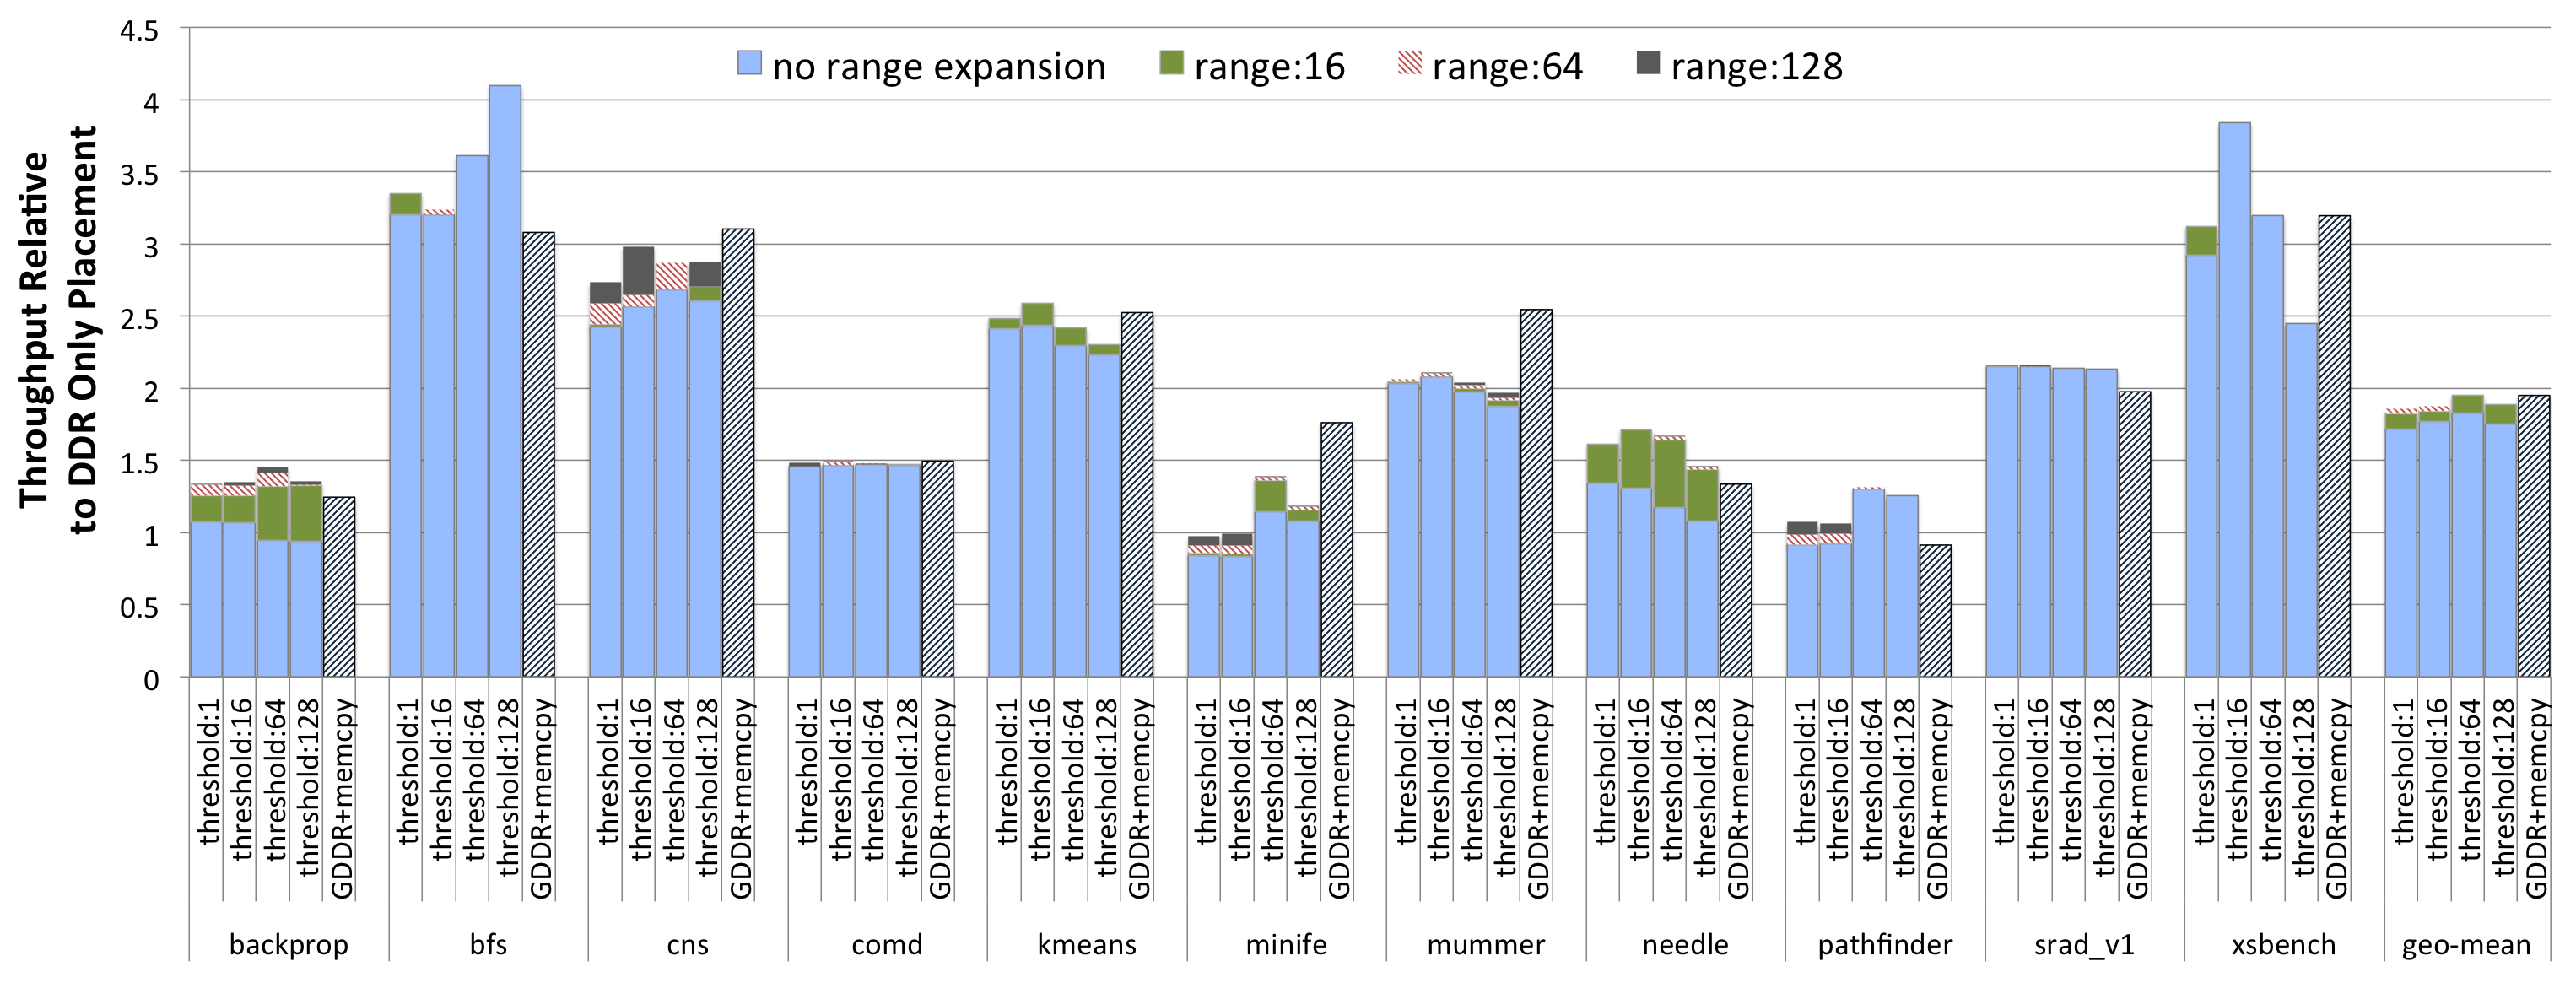
\includegraphics[width=\textwidth]{hpca2015/figures/thresh-rangeExp.png} 
    \caption{Effect of range expansion on workload performance when used in conjunction with threshold based migration.}
    \label{fig:rangeexpansion}
\end{figure*}

Figure~\ref{fig:rangeexpansion} shows application performance as a stacked bar chart on top of the
the baseline threshold-based page migration policy for various range expansion values.
For the different range expansion values, a single migration trigger is expanded to the surrounding 16, 64, or 128 
virtually addressed pages that fall within a single allocation (i.e., were
allocated in the same call to {\tt malloc}).
The pages identified via range expansion are added to the page migration list in order of furthest, 
to nearest pages from the triggered virtual address. Pages that are farther from the (already accessed) trigger
page are less likely to have been touched by the GPU yet and hence are
least likely to be cached in the GPU's TLB. These pages therefore do not
require expensive TLB shootdowns and pipeline stalls.

We see that range expansion allows us to outperform not only CC-NUMA access to DDR, but ---in many cases--- performance
exceeds that of the legacy GDDR+{\tt memcpy} implementation.  These results indicate that aggressive prefetching, 
based on first touch access information, provides a balanced method of using both DDR and GDDR
memory bandwidth.  To understand the improvement 
from the reduction in TLB shootdowns, we report the fraction of 
page migrations that required no TLB shootdown in Table~\ref{tab:shootdowns} (second column).  Compared to  
threshold-based migrations without range expansion, where all migrations incur a TLB shootdown, range expansion 
eliminates 33.5\% of TLB shootdowns on average and as many as 89\% for some applications, drastically 
reducing the performance impact of these shootdowns.

\begin{table}[bh!]
\begin{center}
\begin{small}
\begin{tabular}{|l|c|c|c|}
\hline
Benchmark & Execution & \% Migrations & Exececution\\
          & Overhead of        &Without  & Runtime\\
          & TLB Shootdowns    & Shootdown & Saved\\
\hline
backprop & 29.1\%& 26\% & 7.6\%\\
bfs & 6.7\%&12\% & 0.8\%\\
cns & 2.4\%&20\% & 0.5\%\\
comd & 2.02\%&89\% & 1.8\%\\
kmeans & 4.01\%&79\% & 3.17\%\\
minife & 3.6\%&36\% & 1.3\%\\
mummer & 21.15\%&13\% & 2.75\%\\
needle & 24.9\%&55\% & 13.7\%\\
pathfinder & 25.9\%&10\% & 2.6\%\\
srad\_v1 & 0.5\%&27\% & 0.14\%\\
xsbench & 2.1\%&1\% & 0.02\%\\
\hline
Average & 11.13\%&33.5\% & 3.72\%\\
\hline
\end{tabular}
\caption{Effectiveness of range prefetching at avoiding TLB shootdowns and runtime savings under a 100-cycle TLB shootdown overhead.}
\label{tab:shootdowns}
\end{small}
\end{center}
\end{table}

Figure~\ref{fig:rangeexpansion} shows, for {\tt bfs} and {\tt xsbench}, that range expansion provides minimal
benefit at thresholds $>$ 1. In these benchmarks, the first touches to
contiguous pages are clustered in time, because the algorithms are designed to use blocked access to the key 
data structures to enhance locality. Thus, the prefetching effect of range
expansion is only visible when a page is migrated upon first touch to a
neighboring page, by the second access to a page, all its neighbors have already been accessed 
at least once and there will be no savings from avoiding TLB shootdowns. On the other hand, in benchmarks 
such as {\tt needle}, there is low temporal correlation among touches to neighboring pages.
Even if a migration candidate is touched 64 or 128 times, some of its
neighboring pages may not have been touched, and thus the prefetching
effect of range expansion provides up to 42\% performance improvement even at higher thresholds.

In the case of {\tt backprop}, we can see that higher thresholds perform poorly
compared to threshold 1. Thresholds above 64 are simply too high; most pages are not accessed
this frequently and thus few pages are migrated, resulting in poor GDDR bandwidth utilization.
Range expansion prefetches these low-touch pages to GDDR as well, recouping the performance losses 
of the higher threshold policies and making them perform similar to a first touch migration policy.
For {\tt minife}, previously discussed in subsection~\ref{thresholdresults}, the effect of prefetching
via range expansion is to recoup some of the performance loss due to needless migrations. However,
performance still falls short of the legacy {\tt memcpy} approach, which in effect, achieves perfect prefetching.
Overuse of range expansion hurts performance in some cases. Under the 
first touch migration policy (threshold-1), using range expansion 16, 64, and 128, the worst-case
performance degradations are 2\%, 3\%, and 2.5\% respectively. While not visible in the graph due to the stacked
nature of Figure~\ref{fig:rangeexpansion}, they are included in the geometric mean calculations.

Overall, we observe that even with range expansion, higher-threshold policies
do not significantly outperform the much simpler first-touch policy. 
With threshold 1, the average performance gain with range expansion of 128 is
1.85$\times$.  The best absolute performance is observed when using a threshold of
64 combined with a range expansion value of 64, providing 1.95$\times$ speedup.
We believe that this additional $\approx$5\% speedup over first touch migration with
aggressive range expansion is not worth the implementation complexity of
tracking and differentiating all pages in the system. In the next section, we discuss how
to recoup some of this performance for benchmarks such as {\tt bfs} and {\tt xsbench}, which 
benefit most from using a higher threshold.

\section{Bandwidth Balancing}
In Section~\ref{threshold}, we showed that using a static threshold-based page migration policy alone could
not ideally balance migrating enough pages to maximize GDDR bandwidth utilization while selectively moving
only the hottest data.  In Section~\ref{rangeexpansion}, we showed that informed page prefetching using
a low threshold and range expansion to exploit locality within an application's virtual address space matches or exceeds the performance of a simple threshold-based policy.  Combining low threshold migration with aggressive prefetching drastically
reduces the number of TLB shootdowns at the GPU, reducing the performance overheads of
page migration.  These policies implemented together, however, will continue migrating pages
indefinitely from their initial locations within DDR memory towards the GPU-attached GDDR memory.

\begin{figure}[thp]
\centering
    \subfloat[bfs]{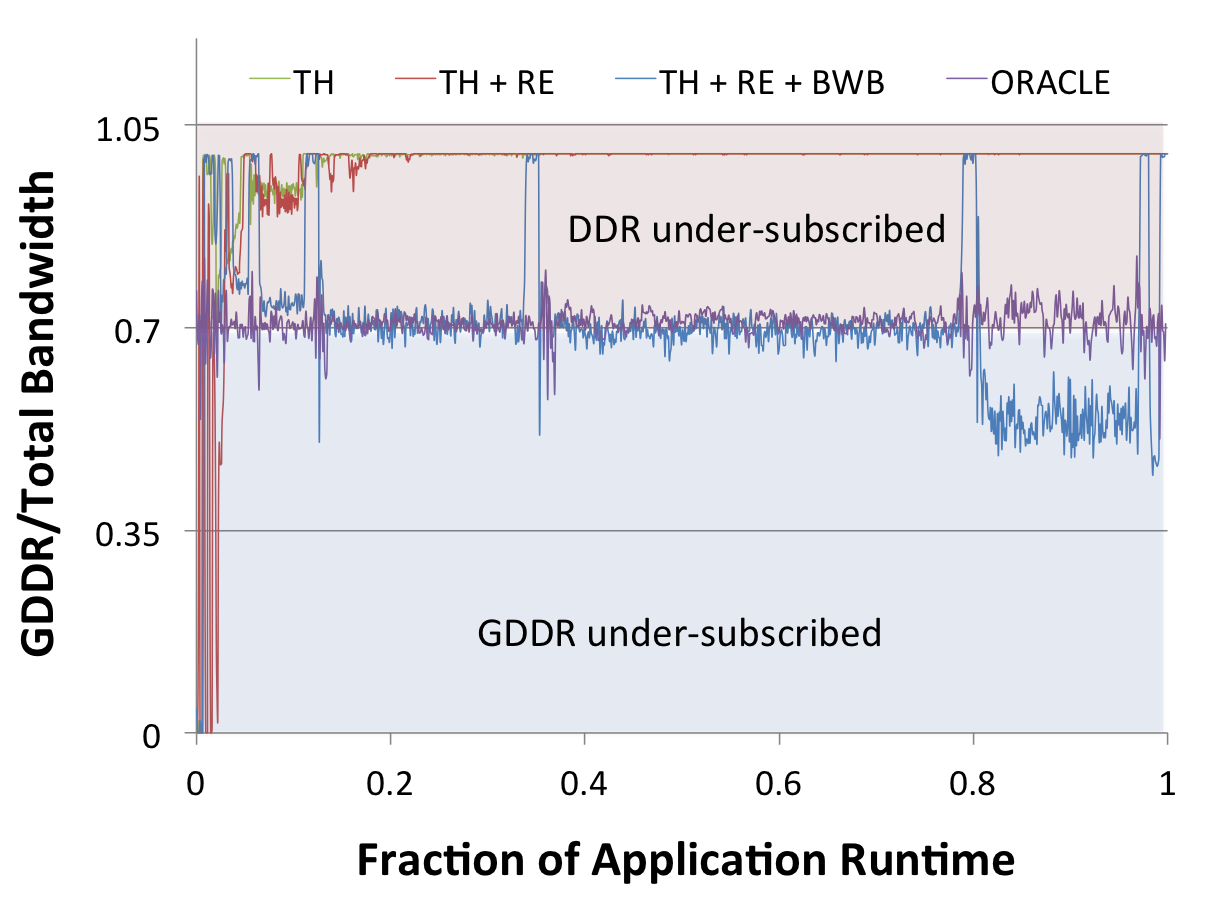
\includegraphics[width=\columnwidth]{hpca2015/figures/bfs-bw-ratio.png}}\\
    \subfloat[xsbench]{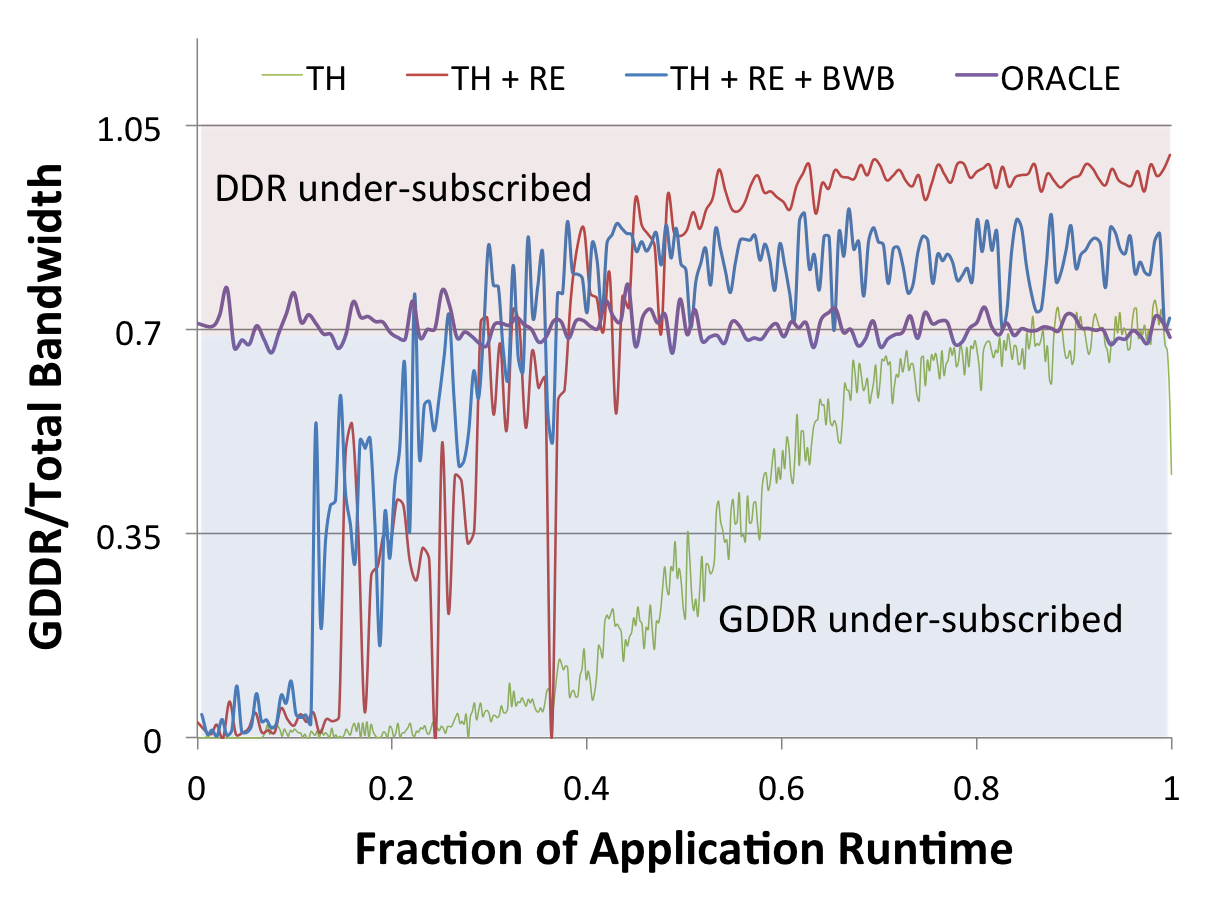
\includegraphics[width=\columnwidth]{hpca2015/figures/xsbench-bw-ratio.png}}\\
    \subfloat[needle]{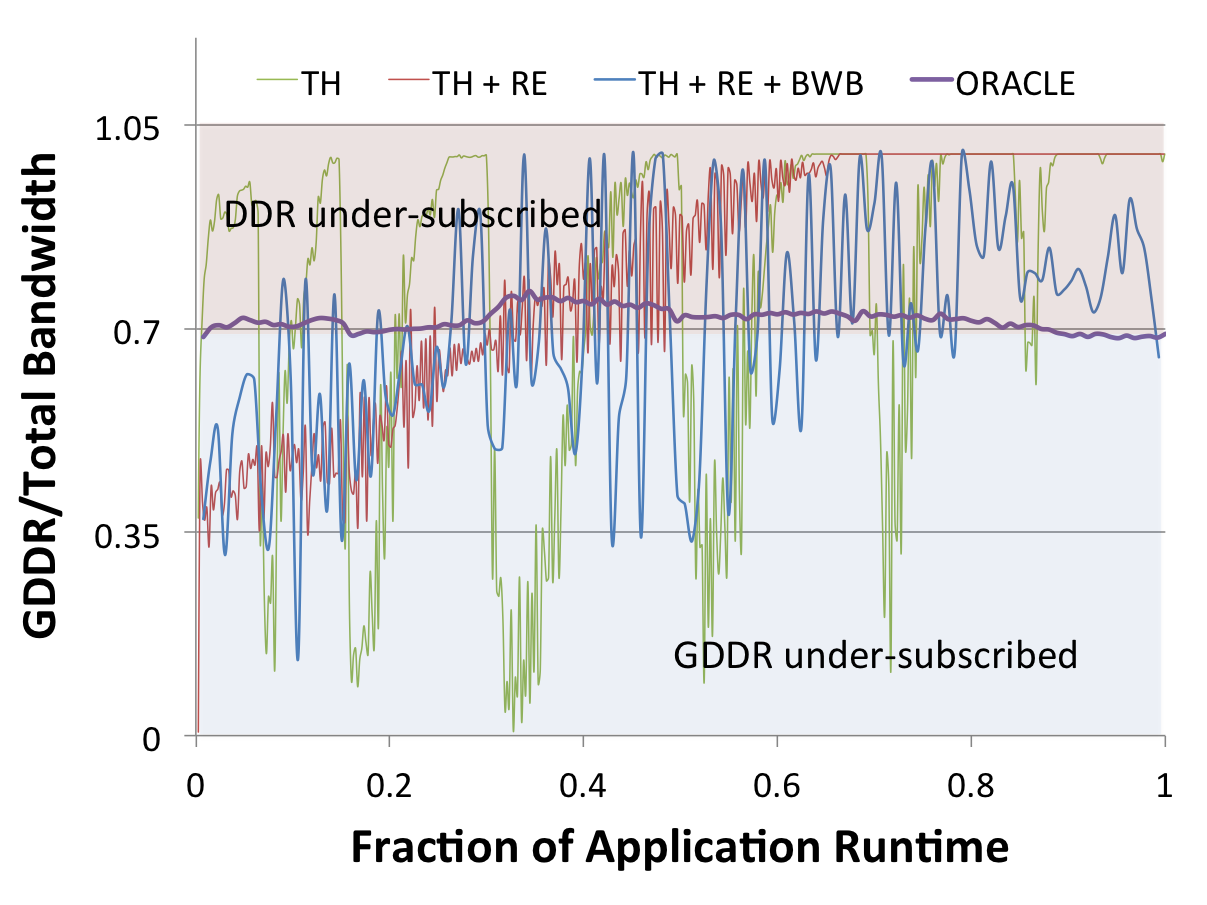
\includegraphics[width=\columnwidth]{hpca2015/figures/needle-bw-ratio.png}}\\
    \caption{Fraction of total bandwidth serviced by GDDR during application
runtime when when using thresholding alone (TH), then adding range expansion
(TH+RE) and bandwidth aware migration (TH+RE+BWB).}
    \label{fig:migrationlimiting}
\end{figure}

As shown in Figure~\ref{fig:threshold}, however, rather than migrating all pages into the GPU memory,
optimal memory bandwidth utilization is achieved by migrating enough pages to GDDR to maximize its bandwidth while
simultaneously exploiting the additional CPU DDR bandwidth via the hardware cache coherence mechanism.  To prevent
migrating too many pages to GDDR and over-shooting the optimal bandwidth target (70\% of
traffic to GDDR and 30\% to DDR for our system configuration), we implement a migration rate control
mechanism for bandwidth balancing.  Bandwidth balancing, put simply, allows aggressive migration while
the bandwidth ratio of GDDR to total memory bandwidth use is low, and rate limits (or eliminates) migration
as this ratio approaches the system's optimal ratio.
We implement a simple bandwidth balancing policy based on a sampled moving average of the
application's bandwidth needs to each memory type.  We assume that the ideal bandwidth ratio in the system can be known either
via runtime discovery of the system bandwidth capabilities (using an application like stream~\cite{stream_benchmark})
or through ACPI bandwidth information tables, much like memory latency information can be discovered today.

Given the bandwidth capability of each interface, we can calculate the ideal fractional ratio, $GDDR / (DDR + GDDR)$, of traffic that should 
target GDDR using the methodology defined by Agarwal et al.~\cite{Agarwal2015}. For the configuration described in Table~\ref{tab:methodology},
this fraction is 71.4\%.  We currently ignore command overhead
variance between the memory interfaces and assume that it is either the same for technologies in use or that
the optimal bandwidth ratio discovered or presented by ACPI will have taken that into account.  Using this target,
our software page migration samples a bandwidth accumulator present for all memory channels every 10,000 
GPU cycles and calculates the average bandwidth utilization of the GDDR and DDR in the system.  If this utilization
is below the ideal threshold minus 5\% we continue migrating pages at full-rate.  If the measured ratio approaches within 5\% of the target
we reduce the rate of page migrations by 1/2.  If the measured ratio exceeds the target, we suspend further migrations.

\begin{figure*}[thp]
    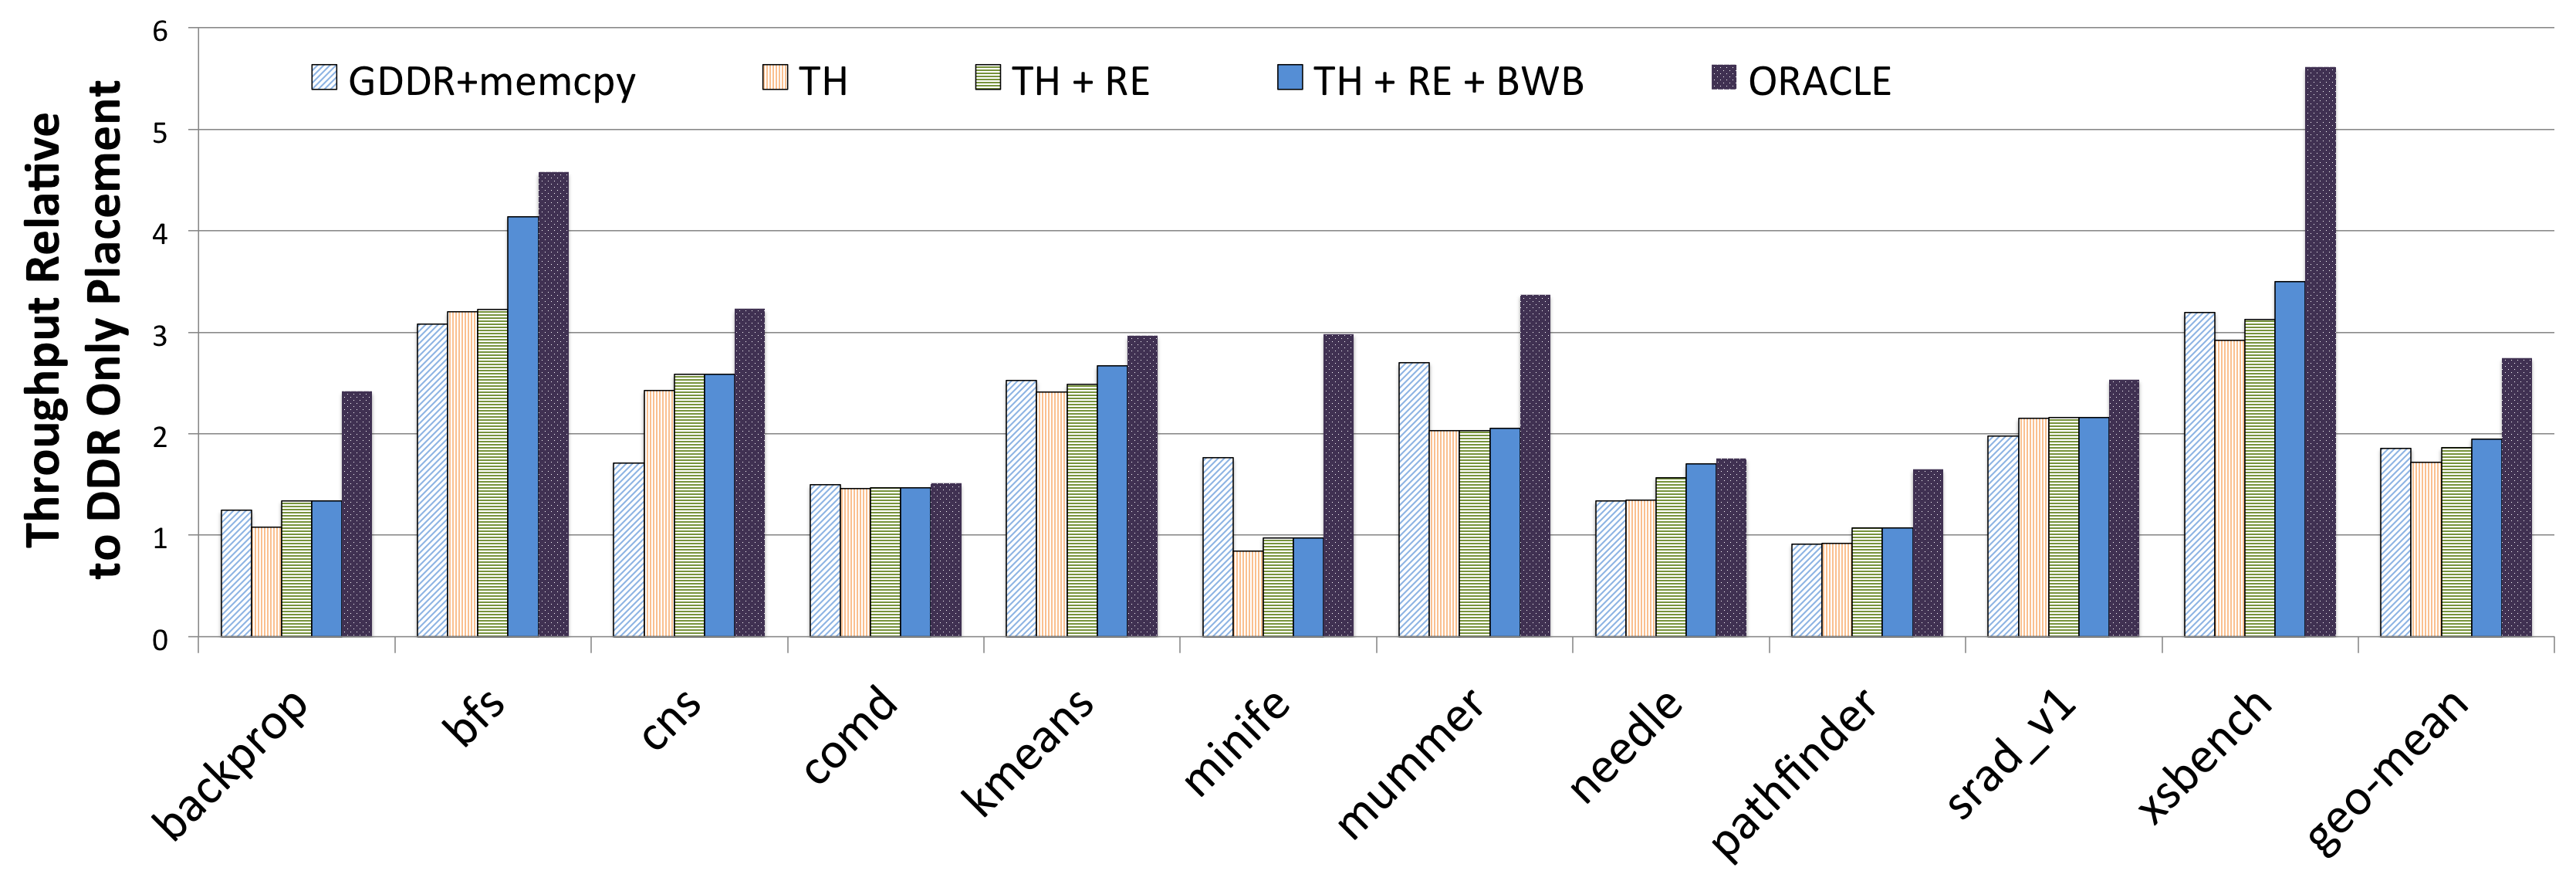
\includegraphics[width=\textwidth]{hpca2015/figures/final.png}
    \caption{Application performance when using thresholding alone (TH), thresholding with range expansion (TH+RE), and thresholding combined with range expansion and bandwidth aware migration (TH+RE+BWB).}
    \label{fig:final}
\end{figure*}

\subsection{Results}
For three example applications, Figure~\ref{fig:migrationlimiting} 
shows the bandwidth utilization of the GDDR versus total bandwidth of the application sampled over time
in 1\% increments.  The $TH$ series provides a view of how migration using single page
migration with a static threshold of one (first touch) performs, while $TH+RE$ shows the static threshold with the range expansion
solution described in Section~\ref{rangeexpansion}, and $TH+RE+BWB$ shows this policy with the addition of our
bandwidth balancing algorithm.  The oracle policy shows that if pages were optimally placed \emph{a priori} before execution there would be some,
but not more than 0.1\% variance in the GDDR bandwidth utilization of these applications.  It is also clear that
bandwidth balancing prevents grossly overshooting the targeted bandwidth ratio, as would happen when using thresholds and range expansion alone.

We investigated various sampling periods shorter and longer than 10,000 cycles, but
found that a moderately short window did not cause unwanted migration throttling during the initial
migration phase but facilitated a quick adjustment of the migration policy once the target bandwidth balance was reached.
If an application's bandwidth utilization subsequently dropped below the target, the short window again enabled rapid
reaction to re-enable migration.   While there is certainly room for further refinement (e.g., enabling 
reverse migration when the DDR memory becomes underutilized), our combined solution of threshold-based migration, prefetching via range expansion, and bandwidth balancing is able to capture the majority of the performance available by balancing page migration
with CC-NUMA access.  Figure~\ref{fig:final} shows the results for our implemented solution across
our benchmark suite.  We see that, on average, we are able to not just improve
upon CPU-only DDR by 1.95$\times$,
but also exceed the legacy up-front {\tt memcpy}-based memory transfer paradigm by 6\%,
and achieve 28\% of oracular page placement.

\begin{figure}[bh!]
    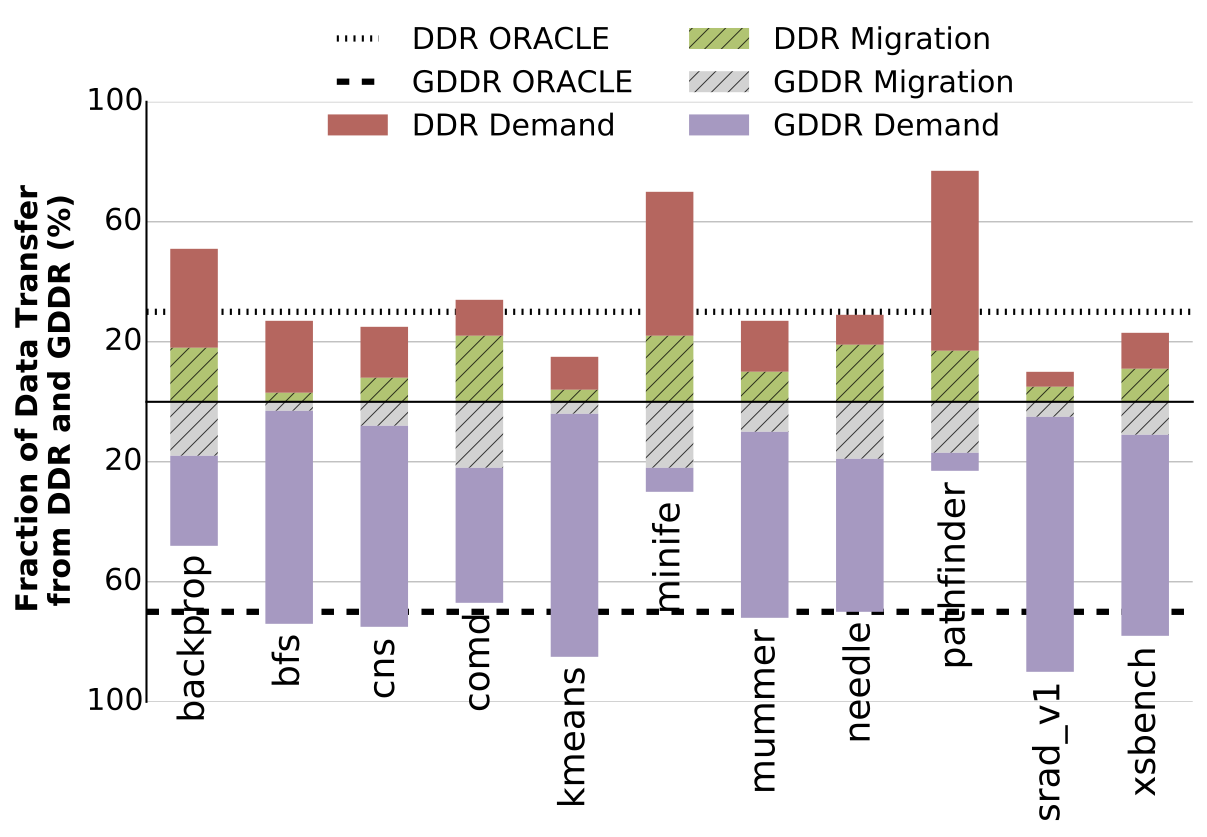
\includegraphics[width=\columnwidth]{hpca2015/figures/bw-util.png}
    \caption{Distribution of memory bandwidth into demand data bandwidth and
migration bandwidth}
    \label{fig:bwutil}
\end{figure}

With our proposed migration policy in place, we seek to understand how it affects the overall bandwidth utilization.  
Figure~\ref{fig:bwutil} shows the fraction of total application bandwidth consumed, divided
into four categories.  The first, DDR Demand is the actual program bandwidth utilization that occurred via CC-NUMA
access to the DDR.  The second and third, DDR Migration and GDDR Migration, are the additional bandwidth overheads on
both the DDR and GDDR that would not have occurred without page migration.  This bandwidth is symmetric because for every read from DDR there is a corresponding write to the GDDR.  Finally, GDDR Demand is the application
bandwidth serviced from the GDDR.  The two additional lines, DDR Oracle and GDDR Oracle, represent
the ideal fractional bandwidth that could be serviced from each of our two memories.

We observe that applications which have the lowest GDDR Demand bandwidth see the least absolute performance improvement from
page migration.  For applications like {\tt minife} and {\tt pathfinder} the GDDR Migration bandwidth also dominates
the GDDR Demand bandwidth utilized by the application. This supports our
conclusion in subsection~\ref{thresholdresults} that migrations may be occurring too late and our mechanisms are not
prefetching the data necessary to make best use of GDDR bandwidth via page migration.  For applications that do perform well 
with page migration, those that perform best tend to have a small amount of GDDR Migration bandwidth when compared to GDDR Demand bandwidth.
For these applications, initial aggressive page migration quickly arrives at the optimal bandwidth balance where our
bandwidth balancing policy then curtails further page migration, delivering good GDDR Demand bandwidth without large migration
bandwidth overhead.

\section{Conclusion}
%In this work, we have examined a pressing problem that the GPU industry is
%facing on how to best handle memory placement for upcoming cache coherent
%GPU-CPU systems.  While the problem of page placement in heterogeneous memories
%has been examined extensively in the context of CPU-only systems, the
%integration of GPUs and CPUs provides several unique challenges.  First, GPUs
%are extremely sensitive to memory bandwidth, whereas traditional memory
%placement decisions for CPU-only systems have tried to optimize latency as
%their first-order concern.  Second, while traditional SMP workloads have the
%option to migrate the executing computation between identical CPUs, mixed
%GPU-CPU workloads do not generally have that option since the workloads (and
%programming models) typically dictate the type of core on which to run.  This
%leaves data migration as the only option for co-locating data and processing
%resources.  Finally, to support increasingly general purpose programming
%models, where the data the GPU shares a common address space with the CPU and
%is not necessarily known before the GPU kernel launch, programmer-specified
%up-front data migration is unlikely to be a viable solution in the future.
%
In this chapter we present a dynamic page migration policy that migrate pages to
GPU-attached high bandwidth memory at application runtime without requiring any
programmer involvement.  
%We have presented a solution to a limited-scope data placement problem for
%upcoming GPU-CPU systems to enable intelligent migration of data into high
%bandwidth GPU-attached memory.  
We identify that demand-based migration alone is unlikely to be a viable
solution due to both application variability and the need for aggressive
prefetching of pages the GPU is likely to touch, but has not touched yet.  The
use of range expansion based on virtual address space locality, rather than
physical page counters, provides a simple method for exposing application
locality while eliminating the need for hardware counters.  
%Developing a system with minimal hardware support is important in the context
%of upcoming GPU-CPU systems, where multiple vendors may be supplying components
%in such a system and relying on specific hardware support on either the GPU or
%CPU to achieve performant page migration may not be feasible.
Our migration solution is able to outperform CC-NUMA access alone by
1.95$\times$, legacy application {\tt memcpy} data transfer by 6\%, and come
within 28\% of oracular page placement.

%These memory migration policies optimize the performance of GPU workloads with
%little regard for CPU performance.  We have shown that intelligent use of the
%high bandwidth memory on the GPU can account for as much as a 5-fold
%performance increase over traditional DDR memory systems.  While this is
%appropriate for applications where GPU performance dominates Amdahl's
%optimization space, applications with greater data sharing between the CPU and
%GPU are likely to evolve.  Understanding what these sharing patterns look like
%and balancing the needs of a latency-sensitive CPU versus a bandwidth-hungry
%GPU is an open problem. Additionally, with memory capacities growing ever
%larger and huge pages becoming more commonly used, evaluating the trade-off
%between reducing TLB shootdowns and longer page copy times will be necessary to
%maintain the high memory bandwidth critical for good GPU performance.



 \chapter{Selective GPU Caches to Eliminate CPU--GPU Cache Coherence}
 \label{chap:hpca2016}
 %\begin{abstract}
The advent of denser/cheaper memory technologies has renewed interest in
two-tiered main memory schemes, where cold data are shifted to slow memory to
enable greater capacity or reduce cost.  Past research on two-tiered main memory
has assumed a 4KB page size.  However, our recent work demonstrates that 2MB
(transparent) huge pages are performance critical in Cloud applications.  We
propose to develop a transparent huge-page-aware two-tiered memory solution,
targeting virtualized cloud applications, which integrates support for dynamic
page migration and transparent huge pages, achieving both the capacity/cost
advantages of two-tiered memory and performance advantages of huge pages. Hot
regions within otherwise cold huge pages present a central challenge to our
objective. We propose translation facades, a 4KB translation that remaps a
portion of a 2MB mapping with an alternate physical address or permissions, to
facilitate remapping hot portions of cold huge pages.
\end{abstract}

\vspace{-.05in}
\section{Introduction}
\label{introduction}

Technology trends indicate an increasing number of systems designed with CPUs, 
accelerators, and GPUs coupled via high-speed 
links. Such systems are likely to introduce unified shared
CPU-GPU memory with shared page tables. In fact, some systems already
feature such implementations~\cite{AMDKaveri}.
Introducing globally visible shared memory
improves programmer productivity by eliminating explicit copies and memory 
management overheads. Whereas this abstraction can be supported using only
software page-level protection mechanisms~\cite{UVM, HSA}, hardware cache coherence 
can improve performance by allowing concurrent, fine-grained access to memory
by both CPU and GPU.  If the CPU and GPU have separate physical
memories, page migration may also be used to optimize page placement for
latency or bandwidth by using both near and far 
memory~\cite{Dashti2013,Agarwal2015b,Meswani2015,Chou2015}.

\begin{figure}[t]
\centering
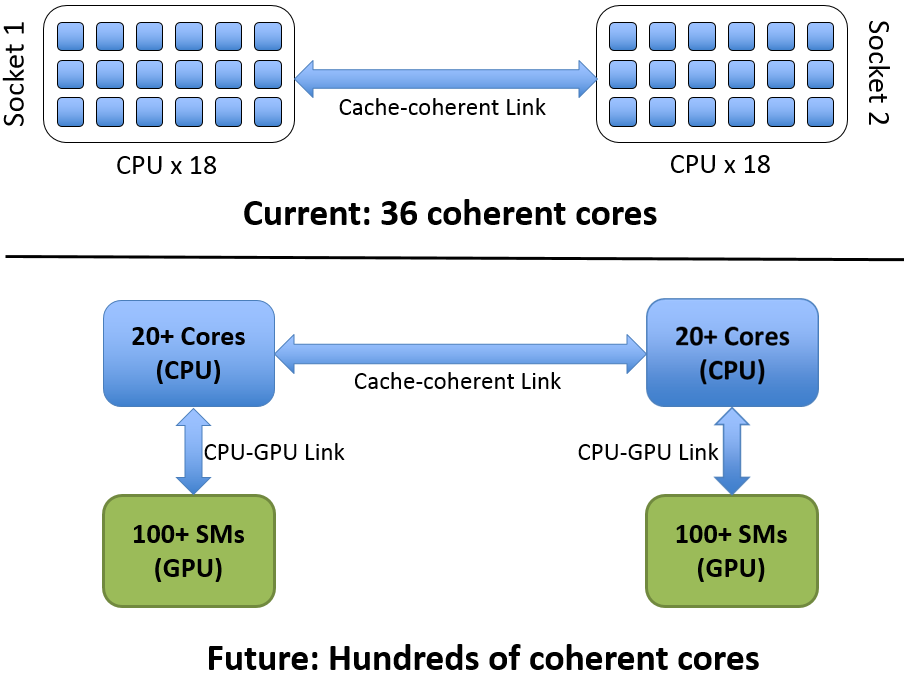
\includegraphics[width=1.0\columnwidth]{hpca2016/figures/coherent_cores.png}
\caption{Number of coherent caches in future two socket CPU-only vs CPU--GPU 
systems.}
\vspace{-0.175in}
\label{fig:motivation}
\end{figure}

Some CPU--GPU systems will be tightly integrated into a system on chip (SoC) making on-chip 
hardware coherence a natural fit, possibly even by sharing a portion of the on-chip 
cache hierarchy~\cite{HSA,AMDAPU,Hechtman2014}.  However, the largest GPU 
implementations consume nearly 8B transistors and have their own 
specialized memory systems~\cite{NVIDIA8BILLION}.  
Power and thermal constraints preclude single-die integration of such designs. 
Thus, many CPU--GPU systems are likely to have 
discrete CPUs and GPUs connected via dedicated off-chip interconnects like 
NVLINK (NVIDIA), CAPI (IBM), HT (AMD), and QPI (INTEL) or implemented as 
multi-chip modules~\cite{NVLINK,CAPI,AMDHT,INTELQPI,Chen92}. The availability of these
high speed off-chip interconnects has led both academic groups and vendors like NVIDIA
to investigate how future GPUs may integrate into existing OS controlled 
unified shared memory regimes used by CPUs~\cite{Pichai2014,Power2014,Agarwal2015,Agarwal2015b}.

Current CPUs have up to 18 cores per socket~\cite{INTELXEONE5V3} but GPUs are
expected to have hundreds of streaming multiprocessors (SMs) each with its own
cache(s) within the next few years. Hence, extending traditional hardware
cache-coherency into a multi-chip CPU-GPU memory system requires coherence
messages to be exchanged not just within the GPU but over the CPU--GPU
interconnect. Keeping these hundreds of caches coherent with a traditional HW
coherence protocol, as shown in Figure~\ref{fig:motivation}, potentially
requires large state and interconnect bandwidth~\cite{Kelm2010,johnson2011}.
Some recent proposals call for data-race-free GPU programming models, which
allow relaxed or scoped memory consistency to reduce the frequency or hide the
latency of enforcing coherence~\cite{Hechtman2014}.  However, irrespective of
memory ordering requirements, such approaches still rely on hardware
cache-coherence mechanisms to  avoid the need for software to explicitly track
and flush modified cache lines to an appropriate scope at each synchronization
point. Techniques like region coherence~\cite{Power2013} seek to scale coherence
protocols for heterogeneous systems, but require pervasive changes throughout
the CPU and GPU memory systems. Such approaches also incur highly coordinated
design and verification effort by both CPU and GPU vendors~\cite{Hong2012} that
is challenging when multiple vendors wish to integrate existing CPU and GPU
designs in a timely manner.

Upcoming GPUs are expected to have hundreds of streaming multiprocessors (SMs),
making the design and verification of hardware cache coherence challenging.
Coherence messages will have to be exchanged across the CPU-GPU interconnect
requiring large states and interconnect bandwidth~\cite{Kelm2010,johnson2011}.
In the past, NVIDIA has investigated extending hardware cache-coherence
mechanisms to multi-chip CPU--GPU memory systems. In this chapter we explore the
techniques to simplify the implementation of shared virtual address space in
heterogeneous CPU-GPU systems by providing the programmers with the hardware
cache coherence while still maintaining performance. We architect a GPU
\textit{selective caching} mechanism, wherein
%Due to the significant challenges associated with building such systems, in this
%work, we architect a GPU \textit{selective caching} mechanism. This mechanism
%provides the conceptual simplicity of CPU--GPU hardware cache coherence and
%maintains a high level of GPU performance, but does not actually implement
%hardware cache coherence within the GPU, or between the CPU and GPU. In our
%proposed selective caching GPU, 
the GPU does not cache data that resides in CPU physical memory, nor does it
cache data that resides in the GPU memory that is actively in-use by the CPU
on-chip caches. This approach is orthogonal to the memory consistency model and
leverages the latency tolerant nature of GPU architectures combined with
upcoming low-latency and high-bandwidth interconnects to enable the benefits of
shared memory.  To evaluate the performance of such a GPU, we measure ourselves
against a theoretical hardware cache-coherent CPU--GPU system that, while high
performance, is impractical to implement.

%In this work, we make the following contributions:
%
%\begin{enumerate}
%\vspace{-.025in}
%\item
%We propose GPU selective caching, which can provide a CPU--GPU system that provides a 
%unified shared memory without requiring hardware cache-coherence protocols within the GPU
%or between CPU and GPU caches.
%\vspace{-.025in}
%\item
%We identify that much of the improvement from GPU caches is due to coalescing 
%memory accesses that are spatially contiguous within a cache line.  Leveraging
%aggressive request coalescing, GPUs can achieve much of the performance benefit
%of caching, without caches.
%\vspace{-.025in}
%\item
%We propose a small on-die CPU cache specifically to handle uncached requests
%that will be issued at sub-cache line granularity from the GPU. This cache helps both 
%shield the CPU memory system from the bandwidth hungry GPU and supports
%improved CPU--GPU interconnect efficiency by implementing variable-sized transfer granularity.
%\vspace{-.025in}
%\item
%We demonstrate that a large fraction of GPU-accessed data is read-only. Allowing 
%the GPU to cache this data and relying on page protection mechanisms rather than hardware 
%coherence to ensure correctness closes the performance gap between a selective
%caching and hardware cache-coherent GPU for many applications.
%\vspace{-.025in}
%\end{enumerate}

%\vspace{-.1in}
\section{Motivation and Background}
\label{background}

Heterogeneous CPU--GPU systems have been widely
adopted by the high performance computing community 
and are becoming increasingly common in other computing paradigms.  High performance GPUs have 
developed into stand-alone PCIe-attached accelerators requiring explicit memory 
management by the programmer to control data transfers into the GPU's 
high-bandwidth locally attached memory. As GPUs have evolved, the onus of 
explicit memory management has been addressed by providing a unified shared
memory address space between the GPU and CPU~\cite{UVM,HSA}.  Whereas a single 
unified virtual address space improves programmer productivity, discrete GPU and 
CPU systems still have separate locally attached physical memories, optimized for 
bandwidth and latency respectively. 

Managing the physical location of data, and guaranteeing that reads access 
the most up-to-date copies of 
data in a unified shared memory can be done through the use of page level 
migration and protection. Such mechanisms move data at the OS page granularity between 
physical memories~\cite{UVM}.  With the advent of non-PCIe high bandwidth, low latency
CPU--GPU interconnects, the possibility of performing cache-line, rather than OS-page-granularity, accesses
becomes feasible.  Without OS level page protection
mechanisms to support correctness guarantees, however,  the responsibility of coherence
has typically fallen on hardware cache-coherence implementations.

\ignore{Managing the physical location and coherence guarantee of 
data in a unified shared memory can be done through the use of page level 
migration and protection, which moves data at the OS page granularity between 
physical memories~\cite{UVM}.  With the advent of non-PCIe high bandwidth, low latency,
CPU--GPU interconnects the possibility of performing cache-line based accesses,
rather than OS page granularity, becomes feasible.  Without OS level page protection
mechanisms to support shared memory guarantees however,  the responsibility of coherence
has typically fallen on hardware cache-coherence implementations.}

\begin{table}[t]
\begin{center}
\begin{tabular}{ddd}
 \hline
 \multicolumn{1}{l}{Workload} &   \multicolumn{1}{c}{L1 Hit Rate (\%)}  &  \multicolumn{1}{c}{L2 Hit Rate (\%)}  \\
 \hline
 \hline
 \multicolumn{1}{l}{backprop}  &   62.4  &   70.0\\
 \hline
 \multicolumn{1}{l}{bfs}  &   19.6  &   58.6  \\
 \hline
 \multicolumn{1}{l}{btree}  &   81.8  &   61.8  \\
 \hline
 \multicolumn{1}{l}{cns}  &   47.0  &   55.2  \\
 \hline
 \multicolumn{1}{l}{comd}  &   62.5  &   97.1  \\
 \hline
 \multicolumn{1}{l}{kmeans}  &   5.6  &   29.5  \\
 \hline
 \multicolumn{1}{l}{minife}  &   46.7  &   20.4  \\
 \hline
 \multicolumn{1}{l}{mummer}  &   60.0  &   30.0  \\
 \hline
 \multicolumn{1}{l}{needle}  &   7.0  &   55.7  \\
 \hline
 \multicolumn{1}{l}{pathfinder}  &   42.4  &   23.0  \\
 \hline
 \multicolumn{1}{l}{srad\_v1}  &   46.9  &   25.9  \\
 \hline
 \multicolumn{1}{l}{xsbench}  &   30.7  &   63.0  \\
 \hline
 \hline
 \multicolumn{1}{l}{Arith Mean}  &   44.4  &   51.6  \\
\hline
\end{tabular}
\caption{GPU L1 and L2 cache hit rates (average).}
\label{tab:gpuhitrate}
\end{center}
\vspace{-.25in}
\end{table}

\begin{figure*}[t]
    \centering
    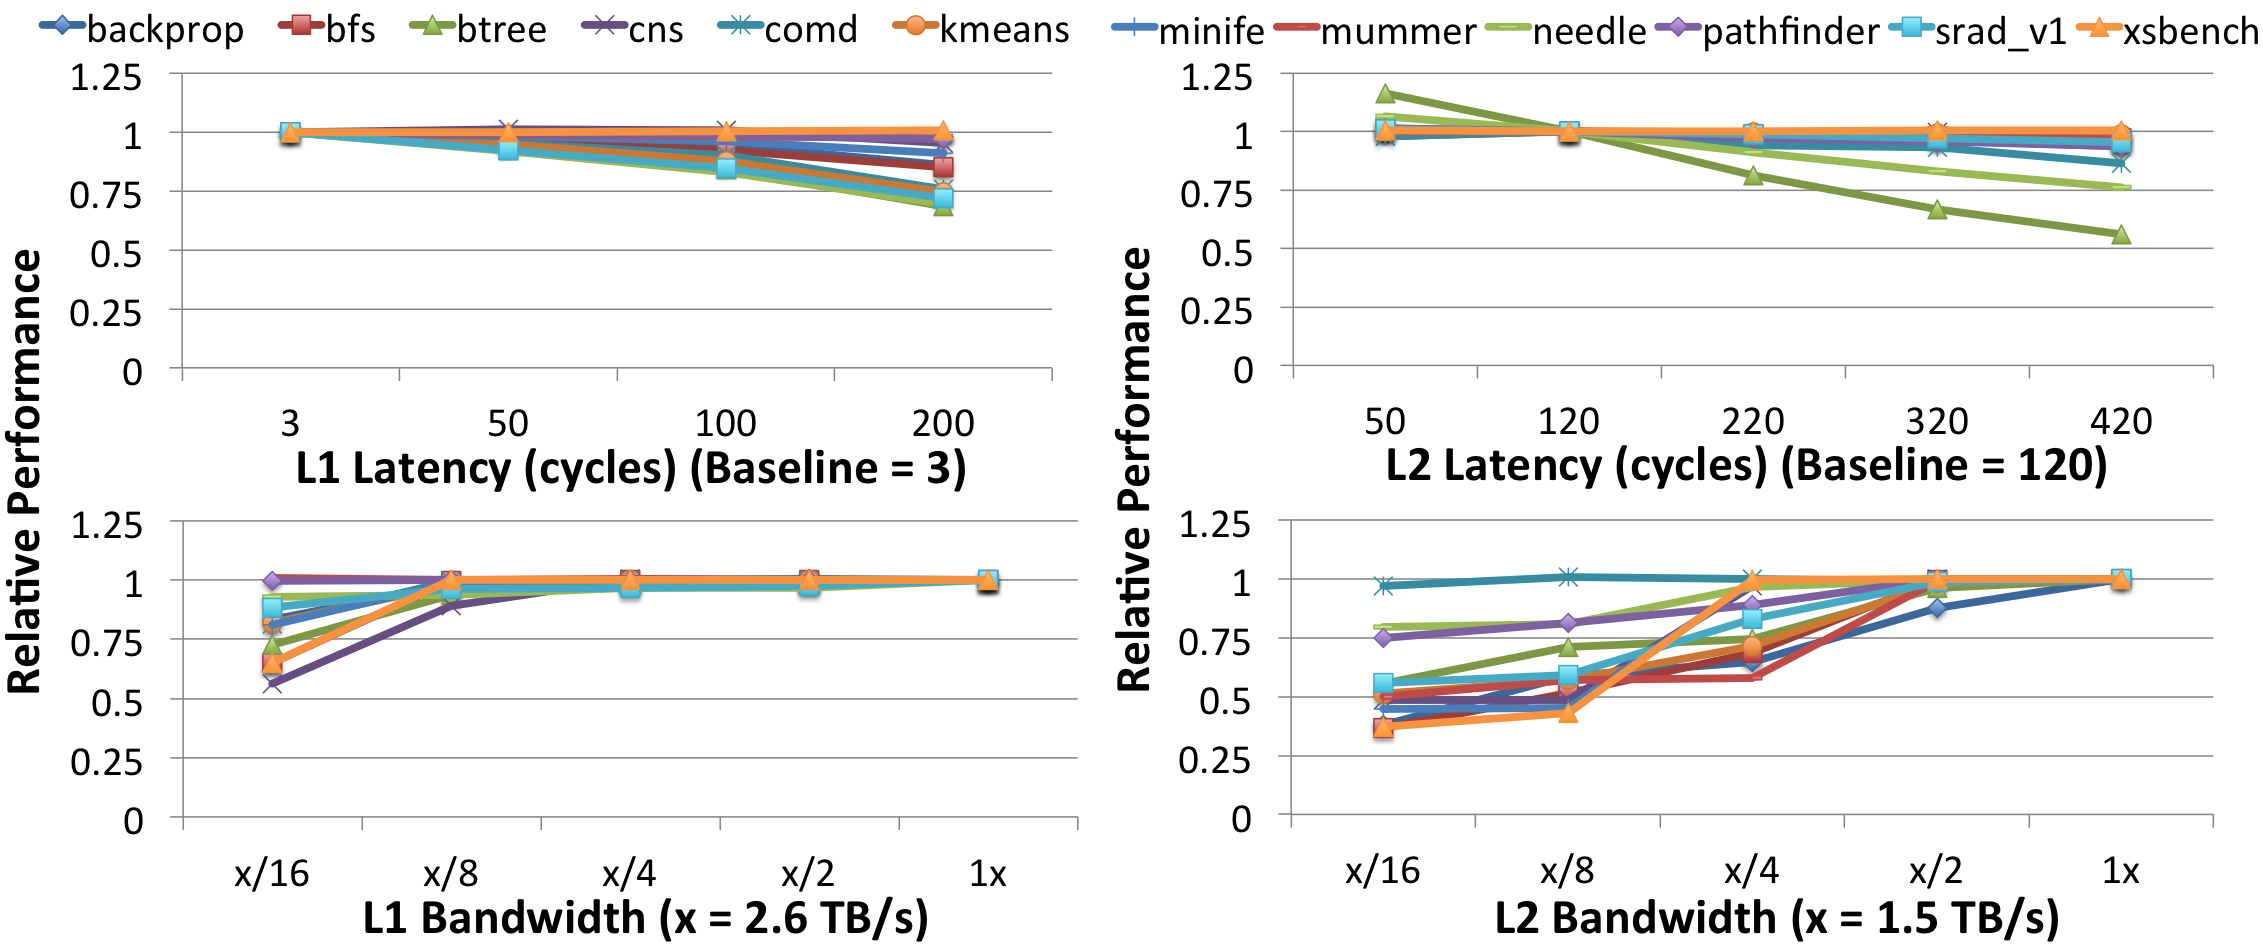
\includegraphics[width=\textwidth]{hpca2016/figures/cache_bw_latency.png}
    \caption{GPU performance sensitivity to L1 and L2 latency and bandwidth
changes.}
    \label{fig:cache_bw_latency}
    \vspace{-.1in}
\end{figure*}

As programming models supporting transparent CPU-GPU sharing become 
more prevalent and sharing becomes more fine-grain and frequent, the 
performance gap between page-level coherence and fine-grained hardware cache-coherent
access will grow~\cite{Agarwal2015,Agarwal2015b,Lim2012}. 
On-chip caches, and thus HW cache coherence, are widely used in CPUs because they 
provide substantial memory bandwidth and latency 
improvements~\cite{Martin2012}.
Building scalable, high-performance cache coherence requires 
a holistic system that strikes a balance between directory storage 
overhead, cache probe bandwidth, and application 
characteristics~\cite{Power2013,Pugsley2010,Cantin2005,johnson2011,Hong2012,Sanchez2012,Kelm2010}.
Although relaxed or scoped consistency models allow coherence operations
to be re-ordered or deferred, hiding latency, they do not obviate the need 
for HW cache coherence. However, supporting a CPU-like HW coherence model
in large GPUs, where many applications do not require coherence, is a tax on GPU designers.  Similarly,
requiring CPUs to relax or change their HW coherence implementations or implement instructions
enabling software management of the cache hierarchy adds significant system complexity.

Prior work has shown that due to their many threaded design, GPUs are 
insensitive to off-package memory latency but very sensitive to off-chip memory 
bandwidth~\cite{Agarwal2015,Agarwal2015b}. Table~\ref{tab:gpuhitrate}
shows the L1 and L2 cache hit rates across a variety of workloads from the Rodinia 
and United States Department of Energy application suites~\cite{Che2009,villa2014}.  These low hit 
rates cause GPUs to also be fairly
insensitive to small changes in L1 and L2 cache latency and bandwidth, as shown in 
Figure~\ref{fig:cache_bw_latency}.  This lack of sensitivity raises the question whether GPUs need 
to uniformly employ on-chip caching of all off-chip memory in order to achieve good performance.  If GPUs do not 
need or can selectively employ on-chip caching, then CPU--GPU systems can be built that
present a unified coherent shared memory address space to the CPU, while not requiring a 
HW cache-coherence implementation within the GPU. 

Avoiding hardware cache coherence benefits GPUs by decoupling them from the coherence protocol 
implemented within the CPU complex, enables simplified GPU designs, and improves
compatibility across future systems. It also reduces the scaling load on the 
existing CPU coherence and directory structures by eliminating the potential addition
of hundreds of additional caches, all of which may be sharing data. Selective caching does not come without
a cost however. Some portions of the global memory space will become un-cacheable
within the GPU\@ and bypassing on-chip caches can place additional load 
on limited off-chip memory resources.  In the following sections, we show that by leveraging
memory request coalescing, small CPU-side caches, improved interconnect efficiency, and
promiscuous read-only caching, selective caching GPUs can perform nearly as well
as HW cache-coherent CPU--GPU\@ systems.

\begin{figure*}[tp]
\centering
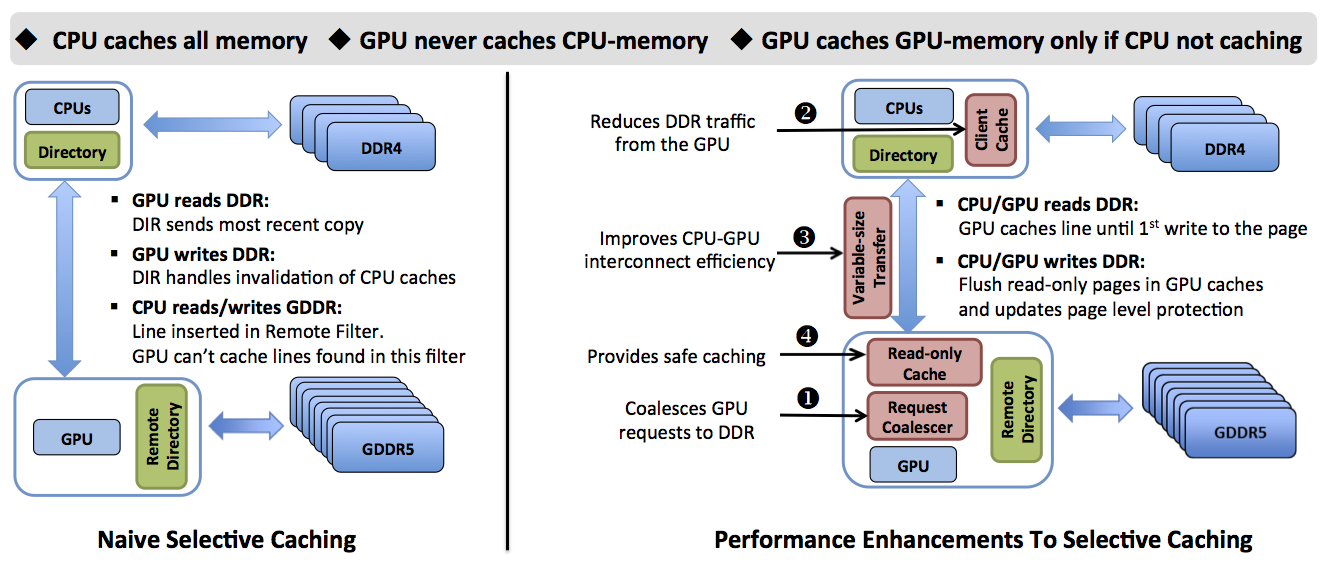
\includegraphics[width=1.0\textwidth]{hpca2016/figures/coherence_overview.png}
\caption{Overview of naive selective caching implementation and optional performance enhancements.
Selective caching GPUs maintain memory coherence with the CPU while not
requiring hardware cache coherence within the GPU domain.}
\label{fig:coherence_overview}
\vspace{.05in}
\end{figure*}

\section{GPU Selective Caching}
\label{proposal}

Historically, GPUs have not required hardware cache coherence because their
programming model did not provide a coherent address space between threads running on separate
SMs~\cite{CUDA7}.  CPUs however, support hardware cache coherence 
because it is heavily relied upon by both system and application
programmers to ensure correctness in multi-threaded programs. 
Existing GPU programming models do not guarantee data correctness when CPU and GPU accesses
interleave on the same memory location while the GPU is executing. One way to
provide such guarantees is to enforce CPU-GPU hardware cache coherence, albeit with significant implementation 
complexity as previously discussed.

Alternatively, if the GPU does not cache any data that is concurrently cached by the CPU,
no hardware coherence messages need to be exchanged between the CPU and GPU, yet data correctness is still guaranteed. 
This approach also decouples
the, now private, coherence protocol decisions in CPU and GPU partitions, facilitating multi-vendor 
system integration.  We now discuss how CPU--GPU
memory can provide this single shared memory abstraction without implementing 
hardware cache coherence. We then propose several micro-architectural enhancements to enable selective caching
to perform nearly as well as hardware cache coherence, while maintaining the programmability benefits of hardware cache coherence.

\subsection{Naive Selective Caching}
\label{naiveselectivecaching}

As shown in Figure~\ref{fig:coherence_overview},
three simple principles enable the GPU to support a CPU-visible shared memory
by implementing selective caching. First, the CPU is always allowed to cache any data in the system regardless 
of whether that data is physically located in the memory attached to the GPU or the CPU\@. 
Second, the GPU is never allowed to cache data that resides within the 
CPU memory.  Finally, the GPU may cache data from its 
own local memory if and only if the CPU is not also caching a copy of this 
data.

When the CPU is known to be caching a line that is homed in GPU memory and the GPU requests
this line, the request must be routed to the CPU where the requested data is serviced 
from the CPU cache, rather than the GPU memory. Similarly, if the GPU is caching a 
line that the CPU requests, then this line must be flushed from the GPU caches when the 
request is received by the GPU memory controller. By dis-allowing caching 
of memory in use by the CPU, the GPU cannot violate the CPU hardware coherence model.

The primary microarchitectural structure needed by the GPU to implement
selective caching is the \emph{remote directory}. The remote directory block
shown in Figure~\ref{fig:coherence_overview} (in green) tracks approximately, but conservatively,
the cache lines homed in GPU  memory that are presently cached at the CPU.
When the CPU requests a line from GPU memory,  its cache block address is  
entered into the remote directory.  If the address was not already present, the GPU
probes and discards the line from all GPU caches, as in a conventional invalidation-based 
coherence protocol.  Once a cache block is added to the GPU remote
directory, it becomes un-cacheable within the GPU; future GPU accesses to the line
will be serviced from the CPU cache.

To limit hardware cost, we implement the remote directory as a cuckoo filter 
(a space efficient version of a counting bloom filter) that never reports
false negatives but may report false positives~\cite{fan2014,bonomi2006}. Thus, the remote directory may erroneously, but conservatively,
indicate that a line is cached at the CPU that has never been requested, but will accurately reference
all lines that have actually been requested.  False positives in the remote directory generate
a spurious request to the CPU, which must respond with a negative acknowledgement (NACK) should the line
not be present in the CPU cache.  This request will then be serviced from the GPU memory
system.  Similarly, if the CPU has cached a line homed in GPU memory (causing a remote directory insertion)
and has since evicted it, the CPU may also NACK a GPU request, causing the request to return to the GPU memory
for fulfillment.

Because entries are inserted but never pruned from our remote directory, we must track if the directory
becomes full or reaches a pre-selected high-water mark.  If it becomes full, our implementation
forces the CPU to flush all cache lines homed in GPU memory and then resets the remote directory.  This limited
cache flush operation  does not flush any lines
homed in CPU memory, the vast majority of the system's memory capacity.  In our
design, the flush is performed by triggering a software daemon to call the Linux \texttt{cacheflush} trap.  

The remote directory is sized to track CPU caching of up to 8MB of GPU memory, which when fully occupied
requires just 64KB of on-chip storage to achieve a false positive rate of 3\%.  In the workloads we evaluate,
the remote directory remains largely empty, and neither the capacity nor false positive rate have a significant
impact on GPU performance.
If workloads emerge that 
heavily utilize concurrent CPU-GPU threads, the size and performance of this structure will need to be re-evaluated. 
However if \texttt{cacheflush} trapping should become excessive due to an undersized remote directory,
page-migration of CPU--GPU shared pages out of GPU memory and into CPU memory can also be employed to 
reduce pressure on the GPU remote directory.

\subsection{Improving Selective Caching Performance}
\label{microarchimprovements}

Caches have consistently been shown to provide significant performance 
gains thanks to improved bandwidth and latency.  As such, naively bypassing the GPU caches based on the mechanisms described in 
Section~\ref{naiveselectivecaching} should be expected to hurt performance. In this subsection we describe 
three architectural improvements that mitigate the impact of selectively bypassing the GPU caches and provide performance approaching
a system with hardware cache coherence.

\subsubsection{Cacheless Request Coalescing}
\label{coalescing}

The first optimization we make to our naive
selective caching design is to implement aggressive miss status handling register (MSHR)
request coalescing for requests sent to CPU memory, labeled \mycirc{1} in Figure~\ref{fig:coherence_overview}.  
Despite not having any cache storage for
requests from CPU-memory, using MSHR-style request coalescing for
read requests can significantly reduce the number of
requests made to CPU memory without violating coherency guarantees.
Request coalescing works by promoting
the granularity of an individual load request (that may be as small as 64 bits)
to a larger granularity (typically 128B cache lines) before issuing the request
to the memory system.  While this larger request is in-flight, if other requests
are made within the same 128B block, then these requests
can simply be attached to the pending request list in the corresponding MSHR and no new request is issued
to the memory system.

To maintain correctness in a non-caching system, this same coalescing
scheme can be utilized, but data that is returned to the coalesced requests for which no pending
request is found, must be discarded immediately. Discarding data in this way is similar to self-invalidating
coherence protocols, which attempt to minimize invalidation traffic in CC-NUMA
systems~\cite{Lebeck95,Lai2000}.  Whereas most MSHR implementations allocate their storage in
the cache into which the pending request will be inserted, our cache-less request coalescing must have
local storage to latch the returned data.  This storage overhead is negligible compared to the aggregate
size of the on-chip caches that are no longer needed with selective caching.

Table~\ref{tab:coalescing_opportunity} shows the fraction of GPU memory requests 
that can be coalesced by matching them to pre-existing in-flight memory requests.
We call request coalescing that happens within a single 
SM \emph{L1 coalescing} and coalescing across SMs \emph{L1+L2 coalescing}.  
On average, 35\% of memory requests can be serviced via 
cacheless request coalescing.  While a 35\% hit rate may seem low when
compared to conventional CPU caches, we observe that capturing spatial request locality
via request coalescing provides the majority of the benefit of the L1 caches (44.4\% hit rate) found
in a hardware cache-coherent GPU, shown in Table~\ref{tab:gpuhitrate}.

\begin{table}[tp]
\begin{center}
\begin{tabular}{ddd}
 \hline
 \multicolumn{1}{l}{Workload}  &  \multicolumn{1}{c}{L1 Coalescing}  &  \multicolumn{1}{c}{L1+L2 Coalescing}  \\
 \hline
 \hline
 \multicolumn{1}{l}{backprop}  &   54.2  &   60.0   \\
 \hline
 \multicolumn{1}{l}{bfs}  &   15.8  &   17.6   \\
 \hline
 \multicolumn{1}{l}{btree}  &   69.4  &   82.4   \\
 \hline
 \multicolumn{1}{l}{cns}  &   24.8  &   28.1   \\
 \hline
 \multicolumn{1}{l}{comd}  &   45.7  &   53.8   \\
 \hline
 \multicolumn{1}{l}{kmeans}  &   0.0  &   0.0   \\
 \hline
 \multicolumn{1}{l}{minife}  &   29.0  &   32.6   \\
 \hline
 \multicolumn{1}{l}{mummer}  &   41.9  &   51.1   \\
 \hline
 \multicolumn{1}{l}{needle}  &   0.1  &   1.8   \\
 \hline
 \multicolumn{1}{l}{pathfinder}  &   41.4  &   45.8   \\
 \hline
 \multicolumn{1}{l}{srad\_v1}  &   30.8   &   34.2   \\
 \hline
 \multicolumn{1}{l}{xsbench}  &   15.6  &   18.0   \\
 \hline
 \hline
 \multicolumn{1}{l}{Average}  &   30.7  &   35.4  \\
\hline
\end{tabular}
\caption{Percentage of memory accesses that can be coalesced into existing 
in-flight  memory requests, when using L1 (intra-SM) coalescing, and L1 + L2 (inter-SM) 
coalescing.}
\label{tab:coalescing_opportunity}
\end{center}
\vspace{-.2in}
\end{table}

\subsubsection{CPU-side Client Cache}
\label{clientcache}

Although memory request coalescing provides hit rates approaching that of
conventional GPU L1 caches, it still falls short as it cannot capture
temporal locality. Selective caching prohibits the GPU from locally caching lines 
that are potentially shared with the CPU but it does not preclude the GPU from remotely 
accessing coherent caches located at the CPU.
We exploit this opportunity to propose a \textit{CPU-side GPU client cache},
labeled \mycirc{2} in Figure~\ref{fig:coherence_overview}.

To access CPU memory, the GPU must already send a request to the CPU
memory controller to access the line. If request coalescing has failed to
capture re-use of a cache line, then multiple requests for the same line will
be sent to the CPU memory controller causing superfluous transfers across the DRAM
pins, wasting precious bandwidth.  To reduce this DRAM pressure we introduce a small 
client cache at the CPU memory controller to service
these GPU requests, thereby shielding the DDR memory system from
repeated requests for the same line.  Our proposed GPU client cache participates in the 
CPU coherence protocol much like any other 
coherent cache on the CPU die, however lines are allocated in this cache only upon 
request by an off-chip processor, such as the GPU\@.

This single new cache does not introduce the coherence and interconnect scaling
challenges of GPU-side caches, but still provides some latency and bandwidth
filtering advantages for GPU accesses. One might consider an alternative where
GPU-requested lines are instead injected into the existing last-level cache
(LLC) at the CPU.  In contrast to an injection approach, our dedicated client
cache avoids thrashing the CPU LLC when the GPU streams data from CPU memory (a
common access pattern).  By placing this client cache on the CPU-side rather
than the GPU-side of the CPU--GPU interconnect, we decouple the need to extend
the CPU's hardware cache coherence protocol into even one on-die GPU cache.
However, because the GPU client cache is located at the CPU-side of the CPU--GPU
interconnect, it provides less bandwidth than a GPU-side on-die cache. As
described in Chapter~\ref{chap:background} and Figure~\ref{fig:cache_bw_latency}
shows, this bandwidth loss may not be performance critical.

\subsubsection{Variable-size Link Transfers}
\label{variablesizing}

Conventional memory systems access data at cache line granularity to 
simplify addressing and request matching logic, improve DRAM energy consumption, and 
exploit spatial locality within caches.  Indeed, the minimum transfer size supported
by DRAM is usually a cache line.  Cache line-sized transfers work well when data
that was not immediately needed can be inserted into an on-chip cache, but
with selective caching, unrequested data transferred from CPU memory must be discarded.  
Hence, portions of a cache line that
were transferred, but not matched to any coalesced access, result in wasted
bandwidth and energy. 

The effect of this data over-fetch is shown in
Table~\ref{tab:overfetch}, where cache line utilization is the fraction of the transferred
line that has a pending request when the GPU receives a cache line-sized response from CPU  memory.
An average cache line utilization of 60\% indicates that just 77 out of 128 bytes transferred are actually used by
the GPU\@. 51 additional bytes were transferred across the DRAM interface and CPU--GPU interconnect 
only to be immediately discarded.

\begin{table}[tp]
\begin{center}
\begin{tabular}{dd}
 \hline
 \multicolumn{1}{l}{Workload}  &  \multicolumn{1}{c}{Avg. Cacheline Utilization(\%)}  \\
 \hline
 \hline
 \multicolumn{1}{l}{backprop}  &   85.9  \\
 \hline
 \multicolumn{1}{l}{bfs}  &   37.4  \\
 \hline
 \multicolumn{1}{l}{btree}  &   78.7  \\
 \hline
 \multicolumn{1}{l}{cns}  &   77.6  \\
 \hline
 \multicolumn{1}{l}{comd}  &   32.6  \\
 \hline
 \multicolumn{1}{l}{kmeans}  &   25.0  \\
 \hline
 \multicolumn{1}{l}{minife}  &   91.6  \\
 \hline
 \multicolumn{1}{l}{mummer}  &   46.0  \\
 \hline
 \multicolumn{1}{l}{needle}  &   39.3  \\
 \hline
 \multicolumn{1}{l}{pathfinder}  &   86.6  \\
 \hline
 \multicolumn{1}{l}{srad\_v1}  &   96.3  \\
 \hline
 \multicolumn{1}{l}{xsbench}  &   30.3  \\
 \hline
 \hline
 \multicolumn{1}{l}{Average}  &   60.6  \\
\hline
\end{tabular}
\caption{Utilization of 128B cache line requests where the returned data 
must be discarded if there is no matching coalesced request.}
\label{tab:overfetch}
\end{center}
\vspace{-.2in}
\end{table}

To address this inefficiency, architects might consider reducing the
transfer unit for cacheless clients from 128B down to 64 or 32 bytes. While 
fine-grained transfers improve transfer efficiency by omitting unrequested data, that
efficiency is offset by the need for multiple small requests and packetization
overhead on the interconnect. For example, in our link implementation,
a transfer granularity of 32B achieves at best 66\% link utilization (assuming
all data is used) due to interconnect protocol overheads, while
128B transfers (again, assuming all data is used) can achieve 88\% efficiency.

To maintain the benefit of request coalescing, but reduce interconnect
inefficiency, we propose using \textit{variable-size transfer units} on the 
CPU--GPU interconnect (labeled \mycirc{3} in Figure~\ref{fig:coherence_overview}).  
To implement variable-size transfer units at the GPU, we allocate GPU MSHR entries at the full
128B granularity; coalescing requests as described in Section~\ref{coalescing}.  However, 
when a request is issued across the CPU--GPU interconnect, we embed a bitmask in the 
request header indicating which 32B sub-blocks of the 128B cache line should be transferred on the return path.
While this initial request is pending across the interconnect, if additional requests
for the same 128B cache line are made by the GPU, those requests will be issued across the interconnect
and their 32B sub-block mask will be merged in the GPU MSHR.  

Similar to the GPU-side MSHR, variable sized transfer units require that the CPU-side client cache also maintain pending MSHR
masks for requests it receives, if it can not service the requests immediately from the
cache.  By maintaining this mask, when the DRAM returns the 128B line, only those
32B blocks that have been requested are transferred to the GPU (again with a bitmask indicating
which blocks are included).  Because there may be
both requests and responses in-flight simultaneously for a single 128B line, it is possible
that two or more responses are required to fulfill the data requested by a single MSHR; the bitmasks
included in each response facilitate this matching.
Because GPUs typically perform SIMD lane-level request coalescing within an SM, 32B requests happen 
to be the minimum and most frequently sized request issued to the GPU memory system.  As a result, we do 
not investigate supporting link transfer sizes smaller than 32 bytes, which would require microarchitectural
changes within the GPU SM.

\subsection{Promiscuous Read-Only Caching}
\label{readonly}

Selective caching supports coherence guarantees by bypassing GPU caches when
hardware cache-coherence operations could be needed.  Thus far, our selective caching architecture
has assumed that the GPU must avoid caching all data homed in CPU memory.  We identify
that we can loosen this restriction and allow GPU caching of CPU memory, but only
if that data can be guaranteed to be read-only by both the CPU and GPU.

Figure~\ref{fig:readonlymotivation} shows the fraction of data touched by the 
GPU that is read-only or both read and written, broken down at 
the OS page (4KB) granularity.  In many workloads, we find the majority 
of the data touched by the GPU is read-only at the OS page level.  We
examine this data at page granularity because, even without hardware 
cache coherence, it is possible (though expensive) to\ignore{ implement coherence}
guarantee correctness through OS page 
protection mechanisms entirely in software. 
Any cache may safely contain data from read-only OS pages.
However, if the page is re-mapped as read-write, cached copies
of the data at the GPU must be discarded, which will occur as part
of the TLB shootdown process triggered by the permission change~\cite{stenstrom1990}.

\begin{figure}[tp]
\centering
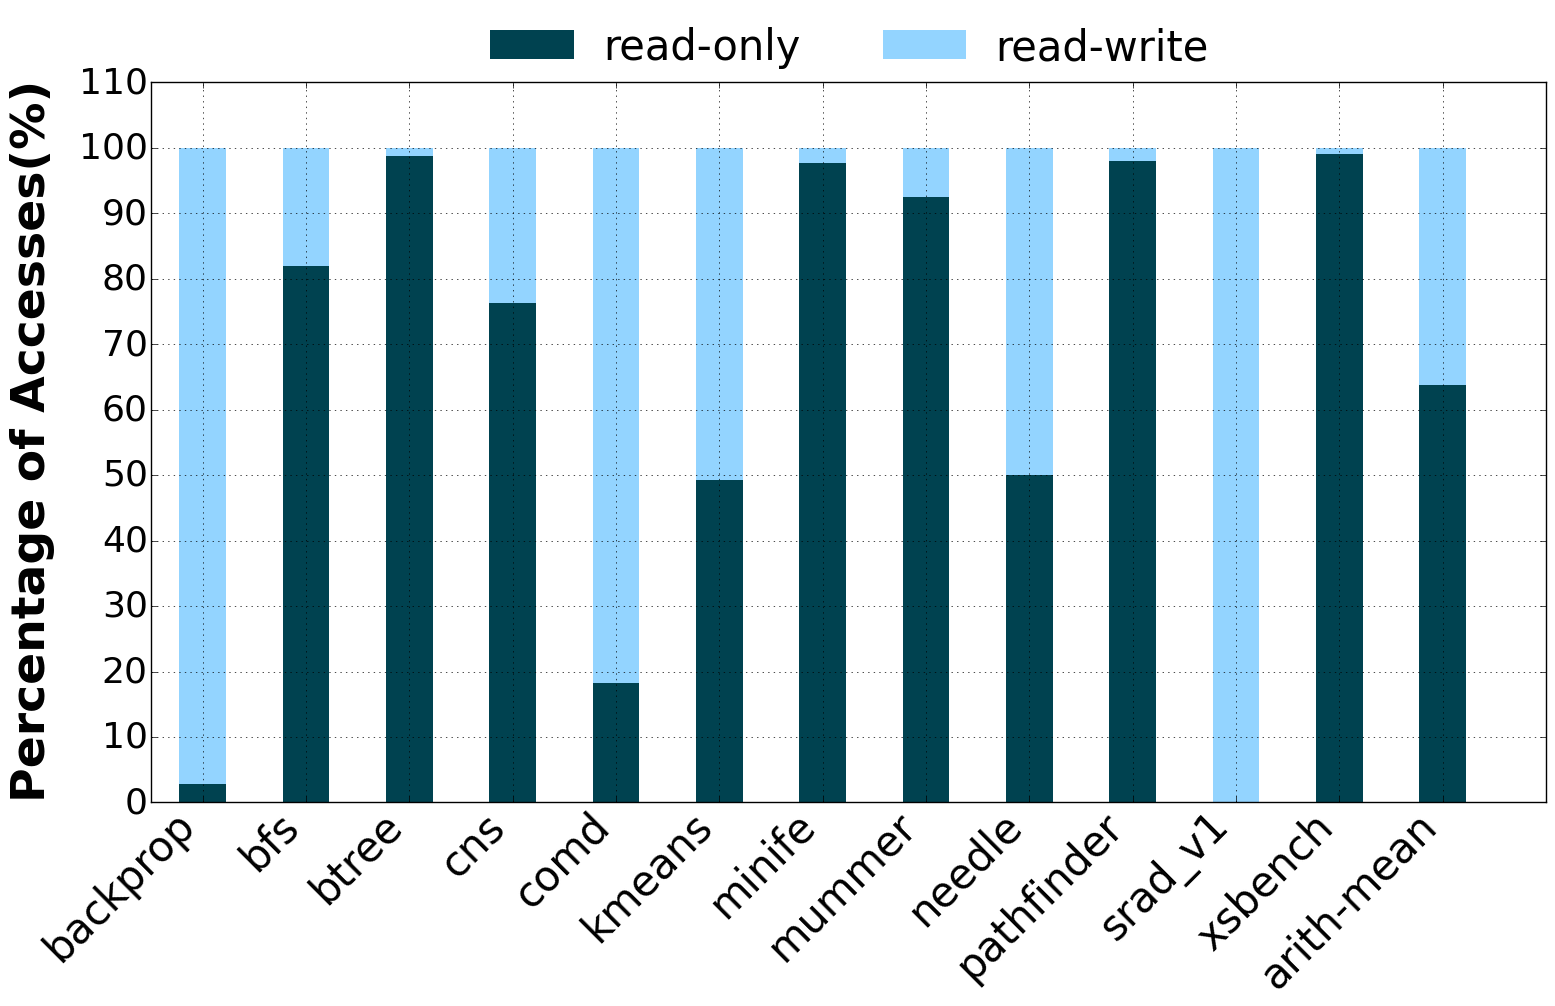
\includegraphics[width=1.0\columnwidth]{hpca2016/figures/read-only.png}
\caption{Fraction of 4KB OS pages that are read-only and read-write
during GPU kernel execution.}
\label{fig:readonlymotivation}
% \vspace{-.1in}
\end{figure}

We propose that despite lacking hardware cache coherence, selective caching GPUs may choose to implement 
\textit{promiscuous read-only caching of CPU-memory}, relying on such page level software coherence 
to provide correctness (labeled \mycirc{4} in Figure~\ref{fig:coherence_overview}).  To implement read-only caching, the GPU software 
run-time system speculatively marks pages within the application as 
read-only at GPU kernel launch time.  It also tracks which pages may have been marked
read-only by the application itself to prevent speculation conflicts.  With pages speculatively
marked as read-only, when the GPU requests pages from the CPU memory, the permissions 
bit in the TLB entry is checked to determine if lines from this page are cacheable by the 
GPU\@ despite being homed in CPU memory. Similarly, if the line resides in GPU memory but is marked as cached by
the CPU in the remote directory, this line can still be cached locally because it is read-only.

If a write to a read-only page occurs at either the CPU or GPU, a protection
fault is triggered. A write by the CPU invokes a fault handler
on the faulting core, which marks the line as read/write at the CPU and
uncacheable at the GPU.  The fault handler then triggers a TLB shootdown,
discarding the now stale TLB entry from all CPU and GPU TLBs.
This protection fault typically incurs a 3-5us delay.  The next access
to this page at a GPU SM will incur a hardware page walk to refetch this PTE, 
typically adding < 1us to the first access to this updated page.

A faulting write at the GPU is somewhat more complex, as protection fault
handlers currently do not run on a GPU SM.  Instead, the GPU MMU must
dispatch an interrupt to the CPU to invoke the fault handler.  That SW handler
then adjusts the permissions and shoots down stale TLB entries, including those at the GPU.
The CPU interrupt overhead raises the total unloaded latency of the fault to ~20us (as measured
on NVIDIA's Maxwell generation GPUs). However, only the faulting warp is stalled: the SM can
continue executing other non-faulting warps.  Once the GPU receives an acknowledgement that the
fault handling is complete, it will re-execute the write, incurring a TLB miss
and a hardware page walk to fetch the updated PTE entry.

The many-threaded nature of the GPU allows us to largely hide 
the latency of these permission faults by executing other warps, thereby mitigating 
the performance impact of the high SW fault latency in nearly all of our workloads.
Nevertheless, software page fault handlers are orders of magnitude more expensive
than hardware cache-coherence messaging and may erode the benefit of promiscuous 
read-only caching if permission faults are frequent.  We evaluate the performance of promiscuous 
caching under different software faulting overhead costs in Section~\ref{readonlyresults}.

\vspace{-.05in}
\section{Methodology}
\label{methodology}

We evaluate selective caching via simulation on a system containing discrete CPUs and GPUs with
DDR4 and GDDR5 memories attached to the CPU and GPU, respectively.  We discuss
our baseline simulation environment in Chapter~\ref{chap:methodology}.
To implement various architectural components we modify our framework 
with simulation parameters shown in Table~\ref{tab:sc-methodology}.
We use bandwidth-aware page placement for all simulations as it has been
shown to be the best page placement strategy without requiring
any application profiling or program modification~\cite{Agarwal2015}. 
In our simulated system, this page placement results in 20\% of the
GPU workload data being placed within the CPU-attached memory with 80\% residing in the GPU-attached
memory.  

In our system, the CPU is connected to the GPU via a full duplex CPU--GPU
interconnect. The interconnect has peak bandwidth of 90GB/s using 16B flits for
both data and control messages with each data payload of up to 128B requiring a
single header flit.  Thus, for example, a 32B data message will require sending
1 header flit + 2 data flits = 3 flits in total.
%To simulate an additional interconnect hop to remote CPU memory, we model an
%additional fixed, pessimistic, 100 cycle interconnect latency to access the
%DDR4 memory from the GPU\@. This overhead is derived from the single additional
%interconnect hop latency found in SMP CPU-only designs, such as the Intel
%Xeon~\cite{INTELXEONE5V3}.
When simulating request coalescing within the GPU, we use the same number of
MSHRs as the baseline configuration but allow the MSHRs to have their own local
return value storage in the cacheless request coalescing case.  The CPU-side GPU
client cache is modeled as an 8-way set associative, write-through, no
write-allocate cache with 128B line size of varying capacities shown later in
Section~\ref{mccache}. The client cache latency is 200 cycles, comprising 100
cycles of interconnect and 100 cycles of cache access latency.  To support
synchronization operations between CPU and GPU, we augment the GPU MSHRs to
support atomic operations to data homed in either physical memory; we assume the
CPU similarly can issue atomic accesses to either memory.

\begin{table}[t]
\begin{center}
\begin{tabular}{|l|l|}
%\hline
%Simulator & GPGPU-Sim 3.x\\
%\hline
%GPU Arch & NVIDIA GTX-480 Fermi-like\\
%\hline
%GPU Cores& 15 SMs @ 1.4Ghz\\
%\hline
%L1 Caches & 16kB/SM, 3 cycle latency\\
%\hline
%L1 MSHRs & 64 Entries/L1\\
%\hline
%L2 Caches & 128kB/Channel, 120 cycle lat.\\
%\hline
%L2 MSHRs & 128 Entries/L2 Slice\\
%\hline
\hline
\multicolumn{2}{|c|}{Memory System}\\
\hline
CPU Client Cache & 512KB, 200 cycle latency\\
\hline
GPU GDDR5 & 8-channels, 336GB/sec aggregate\\
\hline
CPU DDR4& 4-channels, 80GB/sec aggregate\\
\hline
SW Page Faults& 16 concurrent per SM\\
\hline
DRAM Timings & \multicolumn{1}{|l|}{RCD=RP=12, RC=40, CL=WR=12}\\
\hline
DDR4 Burst Len.& 8\\
\hline
\hline
\multicolumn{2}{|c|}{CPU--GPU Interconnect}\\
\hline
Link Latency& 100 GPU core cycles\\
\hline
Link Bandwidth& 90 GB/s Full-Duplex\\
\hline
Req. Efficiency& 32B=66\%, 64B=80\%, 128B=88\%\\
\hline
\end{tabular}
\caption{Parameters for experimental GPGPU based simulation environment.}
\label{tab:methodology}
\end{center}
\vspace{-.1in}
\end{table}

To model promiscuous read-only caching, we initially mark all the pages (4kB in
our system) in DDR as read-only upon GPU kernel launch. When the first write is
issued to each DDR page, the ensuing protection fault invalidates the TLB entry
for the page at the GPU.  When the faulting memory operation is replayed, the
updated PTE is loaded, indicating that the page is uncacheable.  Subsequent
accesses to the page are issued over the CPU--GPU interconnect.  Pages marked
read-write are never re-marked read-only during GPU kernel execution. Using the
page placement policy described earlier in this section, the GPU is able to
cache 80\% of the application footprint residing in GPU memory. We vary our
assumption for the remote protection fault latency from 20-40us and assume
support for up to 16 pending software page protection faults per SM; a
seventeenth fault blocks the SM from making forward progress on any warp.

We evaluate results using the Rodinia and United States Department of Energy
benchmark suites. We execute the applications under the CUDA 6.0 weak
consistency memory model.  While we did evaluate workloads from the
Parboil~\cite{Parboil} suite, we found that these applications have
uncharacteristically high cache miss rates, hence even in the hardware
cache-coherent case, most memory accesses go to the DRAM. As such, we have
chosen to omit these results because they would unfairly indicate that selective
caching is performance equivalent to a theoretical hardware cache-coherent GPU.
In Section~\ref{results} we report GPU performance as application throughput,
which is inversely proportional to workload execution time.

\section{Results}
\label{results}
We evaluate the performance of selective GPU caching through iterative addition of our three proposed microarchitectural
enhancements on top of naive selective caching. We then add promiscuous read-only caching and 
finally present a sensitivity study for scenarios where the workload footprint is too large for a 
performance-optimal page placement split across CPU and GPU memory.

\subsection{Microarchitectural Enhancements}
Figure~\ref{fig:uncachableperformance} shows the baseline performance of naive selective caching
compared to a hardware cache-coherent GPU.  Whereas performance remains as high as 95\% of the baseline 
for some applications,
the majority of applications suffer significant degradation, with applications like \texttt{btree}
and \texttt{comd} seeing nearly an order-of-magnitude slowdown.  The applications that are hurt most
by naive selective caching tend to be those that have a high L2 cache hit rate
in a hardware cache-coherent GPU
implementation like \texttt{comd} (Table~\ref{tab:gpuhitrate}) or those that are highly sensitive to L2 cache latency
like \texttt{btree} (Figure~\ref{fig:cache_bw_latency}).  Prohibiting all caching of CPU 
memory results in significant over-subscription of the CPU
memory system, which quickly becomes the bottleneck for application forward progress, resulting in
nearly a 50\% performance degradation across our workload suite.

\begin{figure}[t]
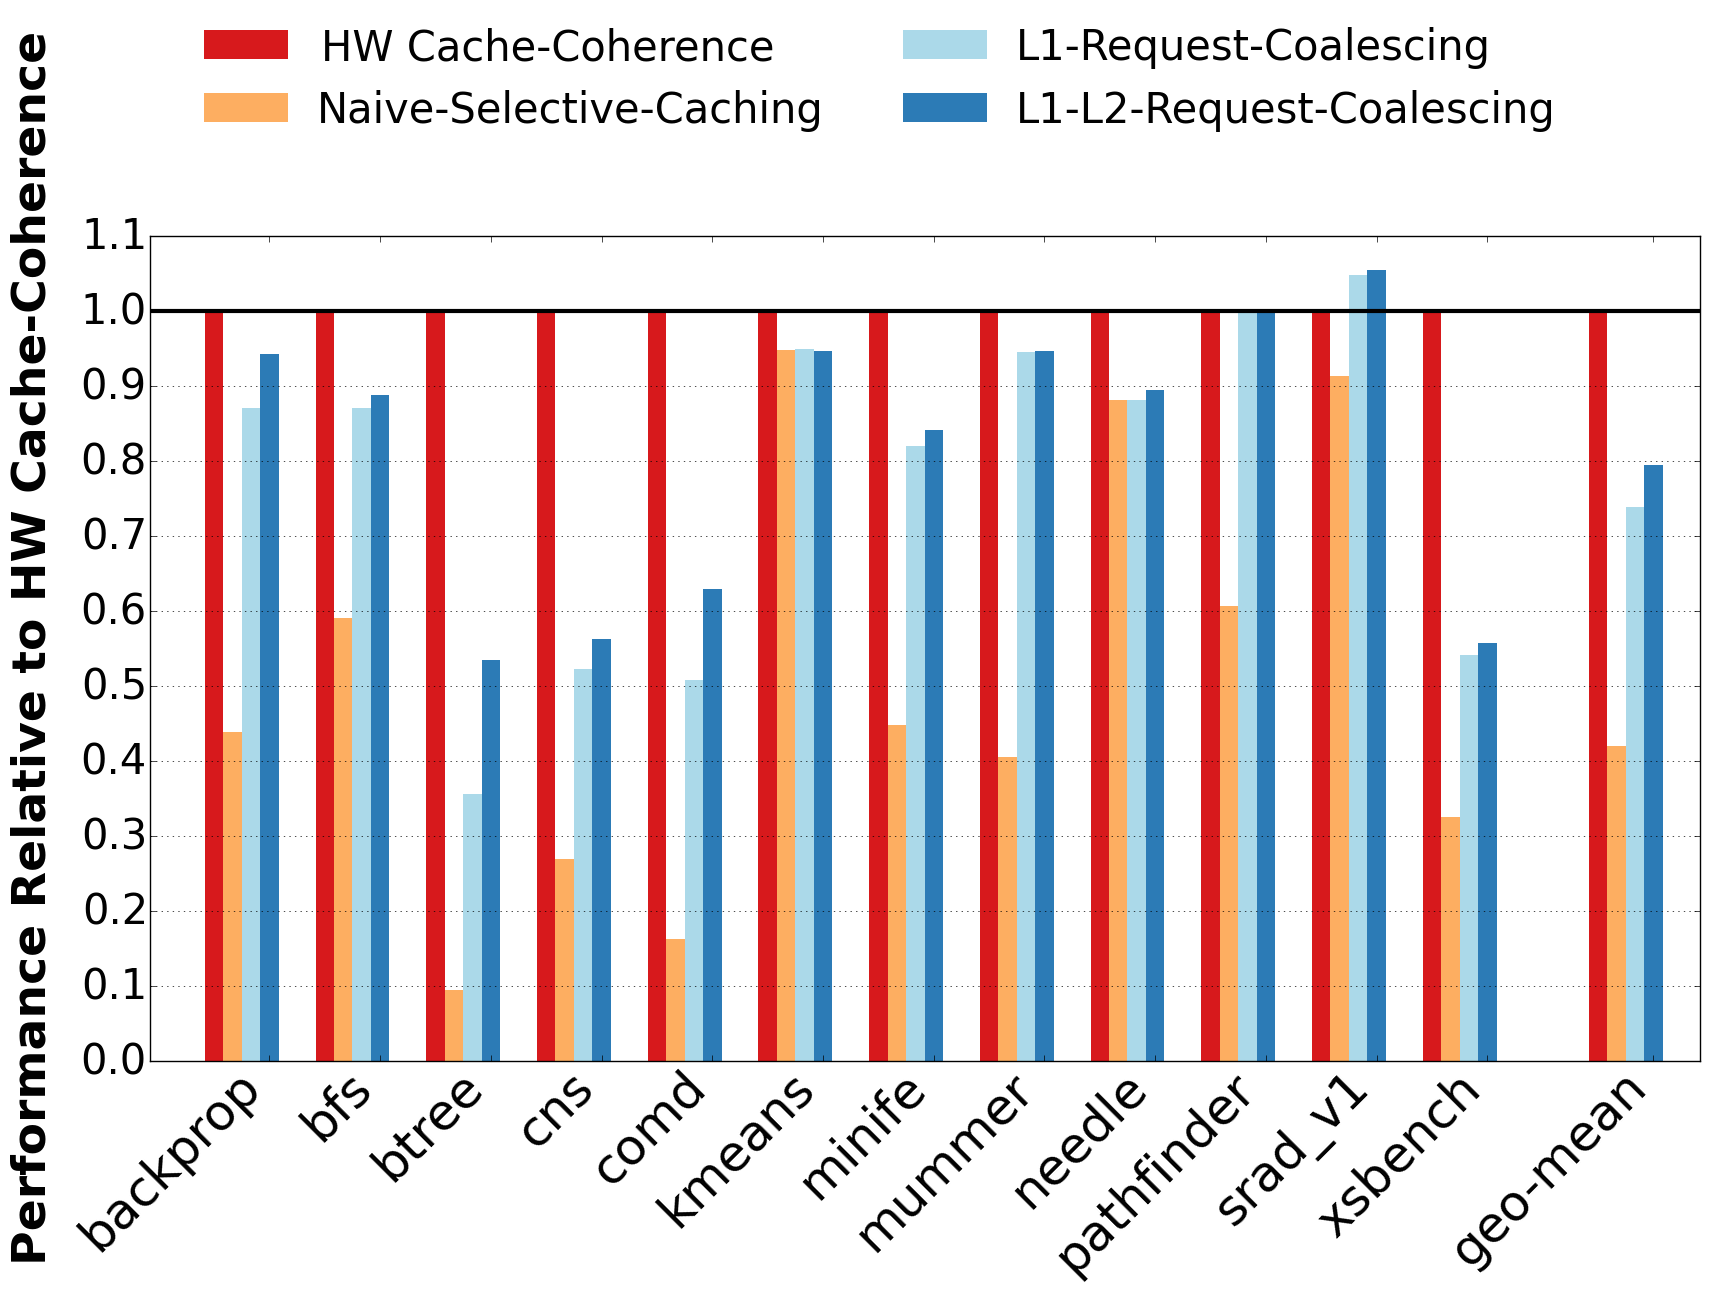
\includegraphics[width=1.0\columnwidth]{hpca2016/figures/unconstrainedperformance.png}
\caption{GPU performance under selective caching with uncoalesced requests, L1 coalesced requests,
L1+L2 coalesced requests.}
\label{fig:uncachableperformance}
\end{figure}

\subsubsection{Cacheless Request Coalescing}
\label{mshrresults}
Our first microarchitectural proposal is to implement cacheless request coalescing as described in Section~\ref{coalescing}.
With naive selective caching relying on only the lane-level request coalescer, performance of the system degrades 
to just 42\% of the hardware cache-coherent GPU, despite only 20\% of the application data residing in CPU physical memory.  
Introducing request coalescing improves performance to 74\% and 79\% of a
hardware cache-coherent GPU
when using L1 coalescing and L1+L2 coalescing, respectively.  This improvement comes from
a drastic reduction in the total number of requests issued across the CPU--GPU
interconnect and reducing pressure on the CPU memory. Surprisingly \texttt{srad\_v1} shows
a 5\% speedup over the hardware cache-coherent GPU when using L1+L2 request coalescing. \texttt{srad\_v1} has 
a large number of pages
that are written without first being read, thus the CPU DRAM system benefits from the elimination of reads that are caused
by the write-allocate policy in the baseline GPU's L2 cache.
Because the request coalescing hit rates, shown in
Table~\ref{tab:coalescing_opportunity}, lag behind the hardware cached hit rates,
selective caching still places a higher load on the interconnect and CPU memory
than a hardware cache-coherent GPU, which translates
into the 21\% performance reduction we observe when using selective caching with aggressive request coalescing.

\begin{figure}[t]
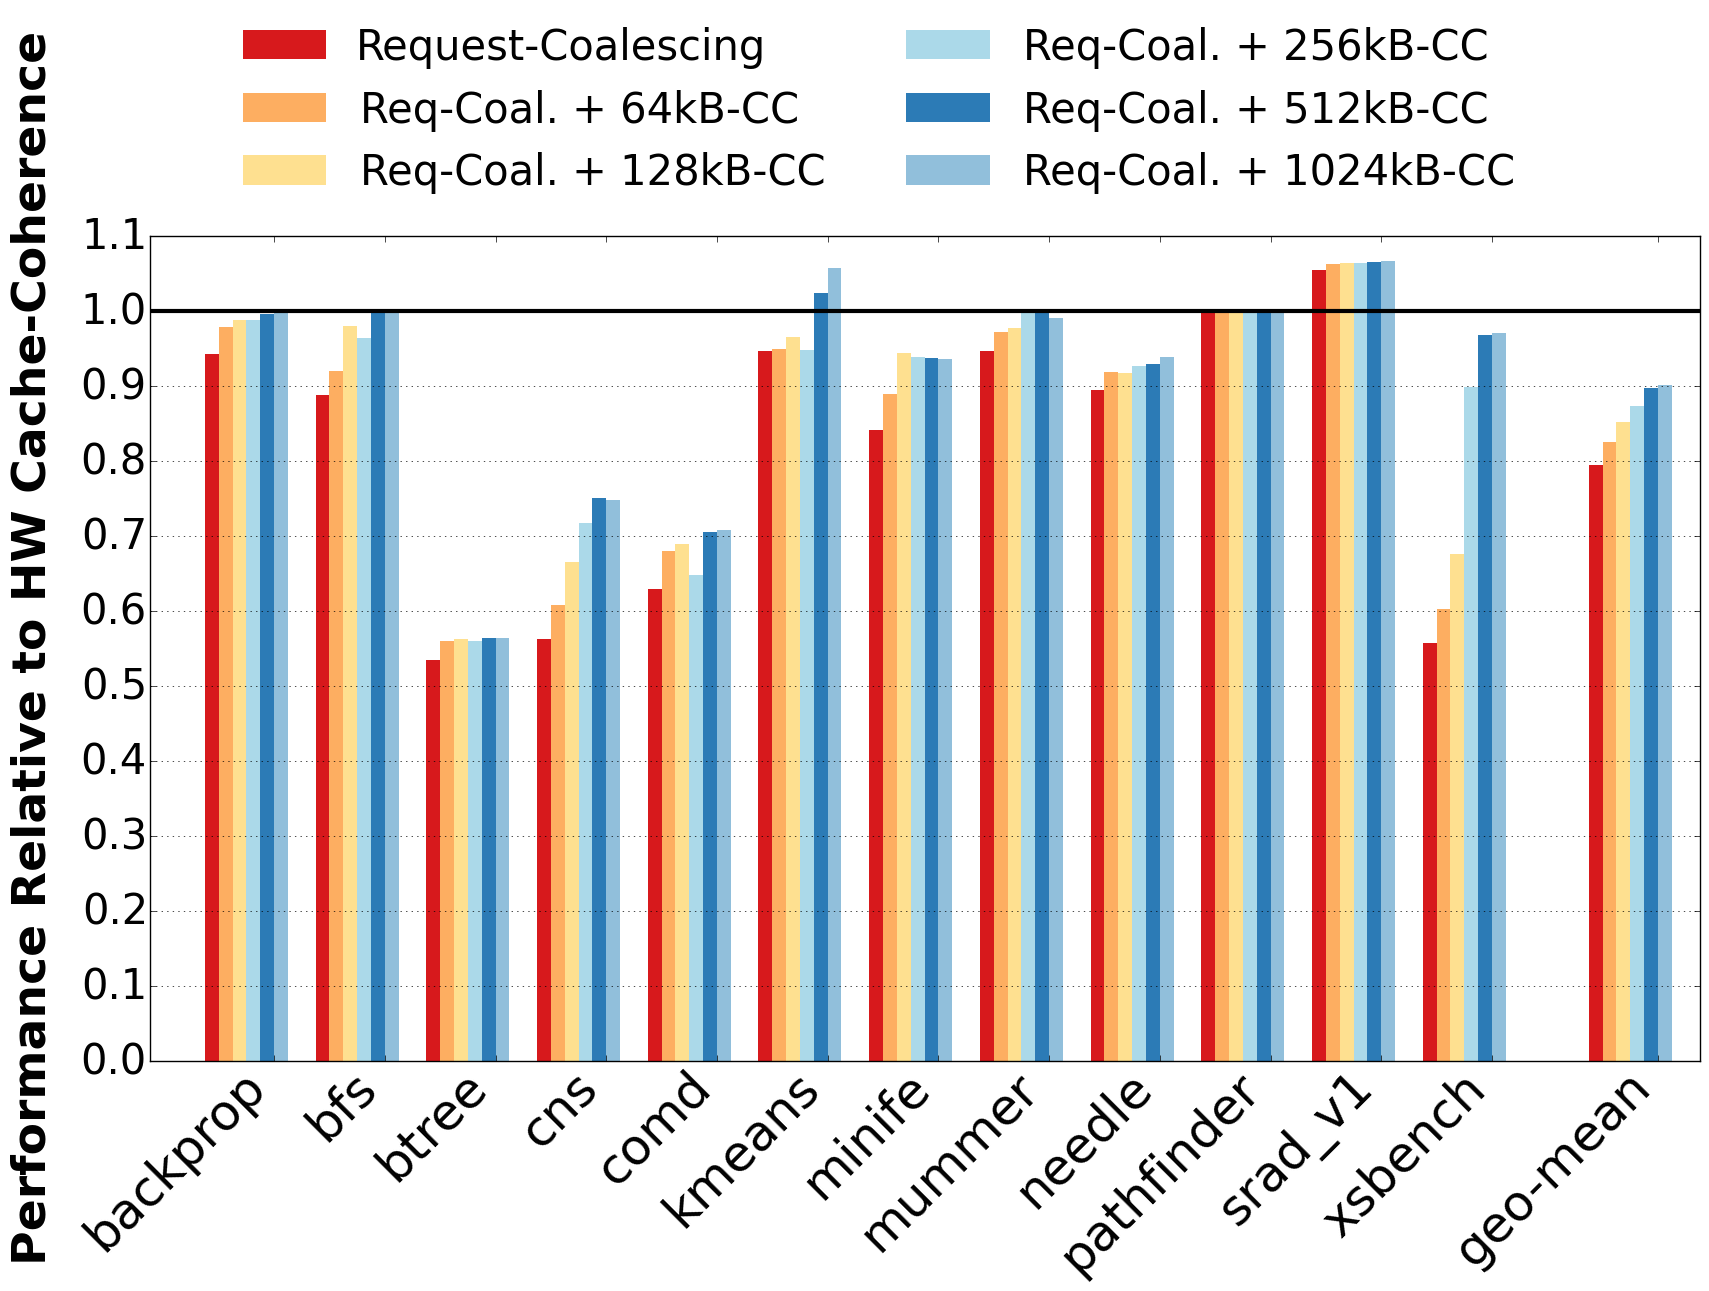
\includegraphics[width=1.0\columnwidth]{hpca2016/figures/unconstrainedperformanceMshrMCCache.png}
\caption{GPU performance with selective caching when combining request coalescing with on CPU-side
caching for GPU clients at 64KB--1MB cache capacities. (CC: Client-Cache)}
\label{fig:mccache}
\end{figure}

\subsubsection{CPU-side Client Cache}
\label{mccache}
Whereas request coalescing captures much of the spatial locality provided by GPU L1 caches, it cannot capture
any long distance temporal locality. Figure~\ref{fig:mccache} shows
the performance differential of adding our proposed CPU-side client cache to L1+L2 request coalescing within the selective
caching GPU. This GPU client cache not only reduces traffic to CPU DRAM from the GPU, but also improves latency for requests
that hit in the cache and provides additional bandwidth that the CPU--GPU interconnect may exploit.  We observe
that performance improvements scale with client cache size up to 512KB before returns diminish.  Combining
a 512KB, 8-way associative client cache with request coalescing improves
performance of our selective caching GPU to within 90\% of the performance of a
hardware cache-coherent GPU\@. Note that \texttt{btree} only benefits marginally from
this client cache because accessing the client cache still requires a round-trip interconnect
latency of 200ns (Section~\ref{methodology}). \texttt{btree} is highly sensitive to
average memory access latency (Figure~\ref{fig:cache_bw_latency}), which is not substantially improved by
placing the client cache on the CPU-die rather than the GPU-die.

The size of an on-die CPU client cache is likely out of the hands of GPU architects, and
for CPU architects allocating on-die resources for an external GPU client may seem an
unlikely design choice.  However, this client cache constitutes only a small fraction of the
total chip area of modern CPUs (0.7\% in 8-core Xeon E5~\cite{XeonLLC2013}) and is the size of just one additional private L2 cache
within the IBM Power 8 processor.  Much like processors have moved towards on-die integration of PCIe to provide improved performance
with external peripherals, we believe the performance improvements due to this cache are significant enough to warrant integration. 
For CPU design teams, integrating such a cache into an existing design is likely easier than achieving performance by extending
coherence protocols into externally developed GPUs. The GPU client cache also need not be specific to just GPU clients,
other accelerators such as FPGAs or spatial architectures~\cite{Putnam2014,Parashar2013} that will be integrated along-side a traditional
CPU architecture will also likely benefit from such a client cache.

\begin{figure}[t]
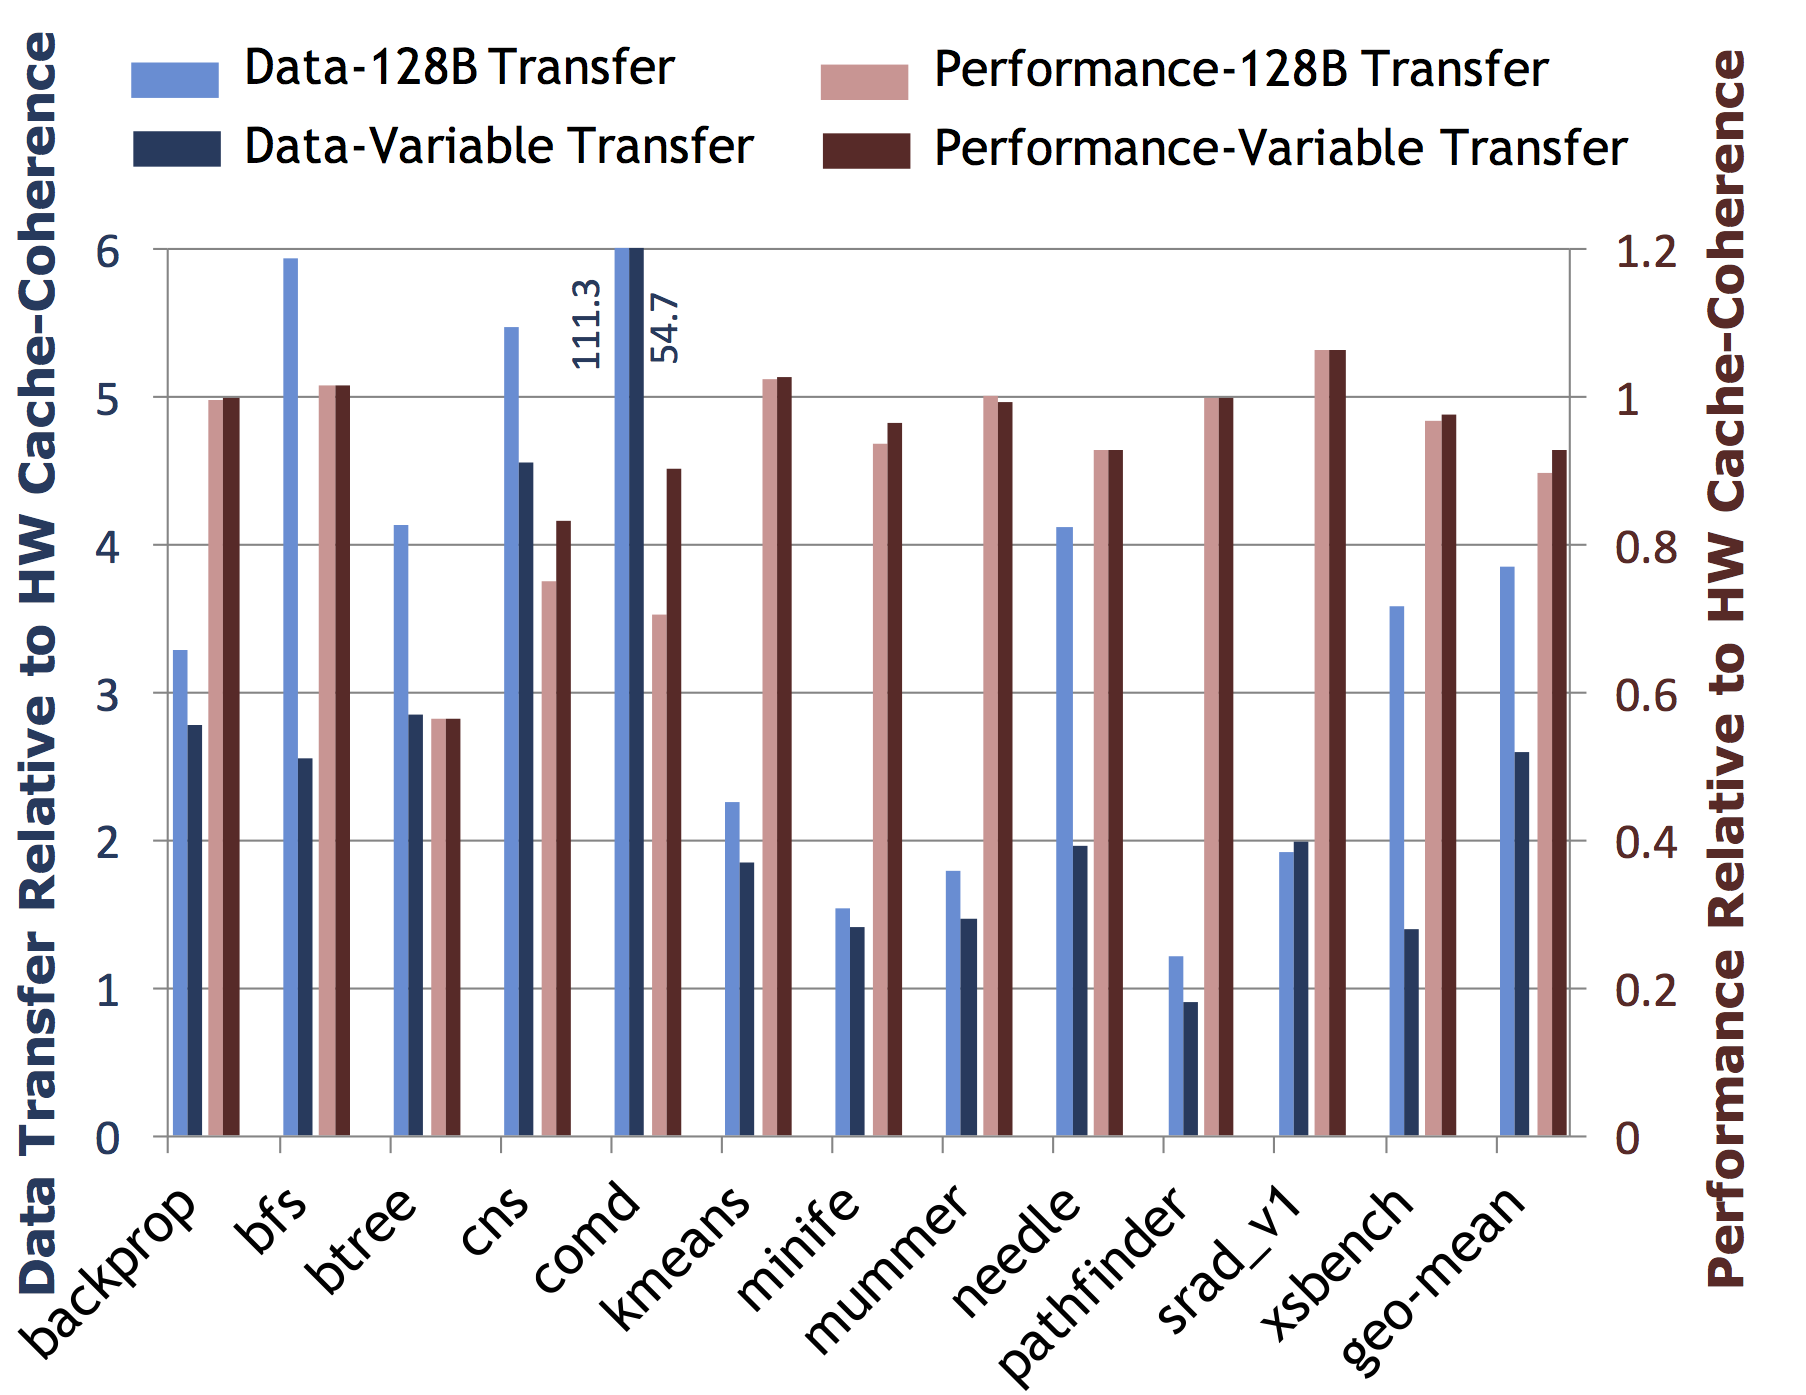
\includegraphics[width=1.0\columnwidth]{hpca2016/figures/linkimprovements.png}
\caption{GPU data transferred across CPU-GPU interconnect (shown left y-axis) and performance (shown right y-axis)
for 128B cache line-size link transfers and variable-size link transfers respectively.}
\label{fig:linkoptimization}
\end{figure}

\begin{figure}[t]
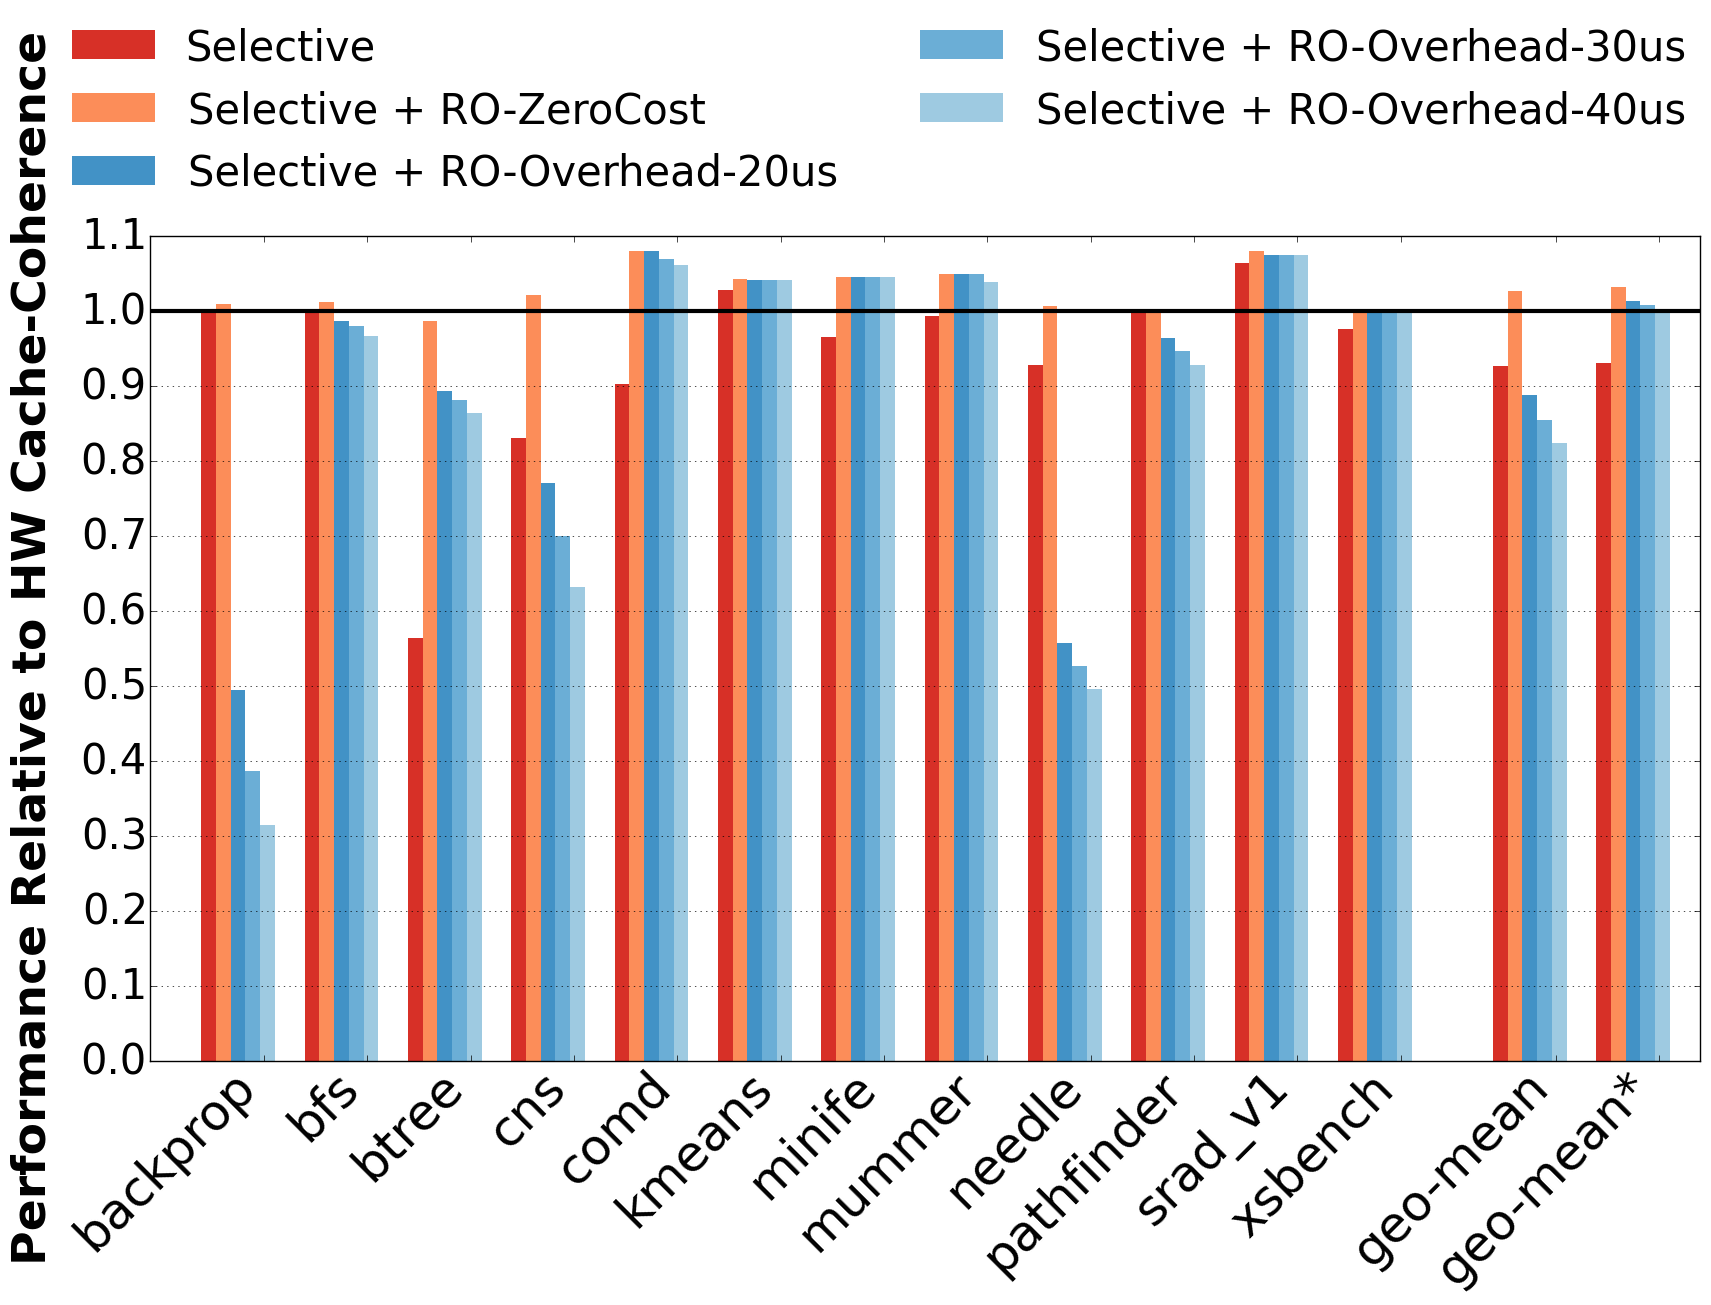
\includegraphics[width=1.0\columnwidth]{hpca2016/figures/readonlycaching.png}
\caption{GPU performance when using Selective caching (Request-Coalescing +
512kB-CC + Variable-Transfers) combined with read-only
based caching. geo-mean*: Geometric mean excluding \texttt{backprop, cns,
needle}, where read-only caching would be switched-off. (RO: Read-Only)}
\label{fig:readonlycaching}
\vspace{-0.1in}
\end{figure}

\subsubsection{Variable-size Link Transfers}
\label{linkoptimization}
Request coalescing combined with the CPU client cache effectively reduce the pressure on the CPU DRAM by limiting
the number of redundant requests that are made to CPU memory.  The CPU client cache exploits temporal locality
to offset data overfetch that occurs on the DRAM pins when transferring data at cache line granularity, but
does not address CPU--GPU interconnect transfer inefficiency.
To reduce this interconnect over-fetch, we propose variable-sized transfer units
(see Section~\ref{variablesizing}). The leftmost two bars for each benchmark in Figure~\ref{fig:linkoptimization} show the total traffic across the
CPU--GPU interconnect when using traditional fixed 128B cache line requests and
variable-sized transfers, compared to a hardware cache-coherent
GPU.  We see that despite request coalescing, our selective caching GPU transfers nearly 4 times the data
across the CPU--GPU interconnect than the hardware cache-coherent GPU.  Our variable-sized transfer
implementation reduces this overhead by nearly one third to just 2.6x more
interconnect traffic than the hardware cache-coherent GPU.

This reduction in interconnect bandwidth results in performance gains of just
3\% on average, despite some applications like {\tt comd} showing significant improvements. 
We observe that variable-sized transfers can significantly improve bandwidth utilization
on the CPU--GPU interconnect but most applications remain performance-limited by the CPU memory 
bandwidth, not the interconnect itself. When we increase interconnect bandwidth by 1.5x without enabling variable-sized
requests, we see an average performance improvement of only 1\% across our benchmark suite.
Variable-sized requests are not without value, however;
transferring less data will save power or allow this expensive off-chip interface to be clocked at a lower
frequency, but evaluating the effect of those improvements is beyond the scope of this work.

\subsection{Promiscuous GPU Caching}
\label{readonlyresults}
By augmenting selective caching with request coalescing, a GPU client cache, and variable-sized transfers,
we achieve performance within 93\% of a hardware cache-coherent GPU\@. 
As described in Section~\ref{readonly}, the GPU can be allowed to cache CPU memory that is contained
within pages that are marked as read-only by the operating system. The benefit of caching data
from such pages is offset by protection
faults and software recovery if pages promiscuously marked as read-only 
and cached by the GPU are later written.
Figure~\ref{fig:readonlycaching} (RO-ZeroCost) shows the upper bound on possible improvements from read-only 
caching for an idealized implementation that marks all pages as read-only and transitions them to
read-write (and thus uncacheable)
without incurring any cost when executing the required protection fault handling routine.  In a few cases, 
this idealized implementation can outperform 
the hardware cache-coherent GPU because of the elimination of write allocations in the GPU caches,
which tend to have little to no reuse.

We next measure the impact of protection fault cost, varying the unloaded fault latency from
20us to 40us (see Figure~\ref{fig:readonlycaching}) which is available on today's GPU implementations.
While a fault is outstanding, the faulting warp and any other warp that accesses
the same address are stalled; but, other warps may proceed, mitigating the impact of these faults on SM forward progress.  
The latency of faults can can be hidden if some warps executing on an SM are reading
this or other pages.  However, if all warps issue writes at
roughly the same time, the SM may stall due to a lack of schedulable warps or MSHR
capacity to track pending faults. When accounting for fault overheads, 
our selective caching GPU with promiscuous read-only caching achieves only 89\% of the performance of the 
hardware cache-coherent GPU.

When using a 20us fault latency, we see that 7 of 12 workloads 
exhibit improvement from read-only caching
and that \texttt{btree} sees a large 35\% performance gain from promiscuous read-only caching
as it benefits from improvements to average memory
access latency.
In contrast, three workloads, \texttt{backprop}, \texttt{cns}, and
\texttt{needle}, suffer considerable slowdowns due to exposed protection fault latency.
These workloads tend to issue many concurrent writes, exhausting the GPUs
ability to overlap execution with the faults.  For such workloads, we advocate
disabling promiscuous read-only caching in software (e.g., via a mechanism that tracks
the rate of protection faults, disabling promiscuous read-only caching when the rate
exceeds a threshold).

In summary, the effectiveness of promiscuous read-only caching depends heavily on
the latency of protection faults and the GPU microarchitecture's ability to overlap the
execution of non-faulting warps with those faults,
which can vary substantially across both operating systems and architectures.  In
systems where the fault latency is higher than the 20us (as measured on current NVIDIA systems), more
judicious mechanisms must be used to identify read-only pages (e.g.,
explicit hints from the programmer via the \texttt{mprotect} system call.)

\subsection {Discussion}
One use case in the future
may be that GPU programmers will size their application's data to extend well beyond
the performance-optimal footprint in CPU and GPU memory.  With excess data spilling over
into the additional capacity provided by the CPU memory, performance
bottlenecks will shift away from the GPU towards the CPU memory system.  In such
cases, the GPU caching policy for CPU memory will come under additional pressure due to
the increased traffic skewed towards CPU memory.

To understand how selective caching affects performance under such a scenario, we evaluate
a situation wherein the application data has been
sized so that 90\% of the footprint resides in CPU memory and just 10\% can fit within GPU memory, as compared to the nearly
inverse performance-optimal 20\%-80\% ratio.
Figure~\ref{fig:capacityconstrained} shows the performance of this memory-capacity-constrained case relative 
to the baseline optimal ratio.  We see that naive selective caching and
our proposed enhancements follow the same trend of performance improvements
shown previously in Section~\ref{results}.  Because this scenario is primarily limited
by the CPU memory system, we see that in some cases the client cache and variable sized transfer interconnect optimizations
can actually outperform the hardware cache-coherent GPU due to a reduction in data overfetch between the CPU memory and the GPU client.
To validate our observation, we added the same client cache and variable
transfers to the hardware cache-coherent baseline configuration and saw an average
speedup of 4.5\%.  Whereas the absolute
performance achieved, compared to a performance-optimal memory footprint and allocation, may not always be compelling, should
software designers chose to partition their problems in this way, we believe selective caching will continue to 
perform as well as a hardware cache-coherent GPU.


\begin{figure}[t]
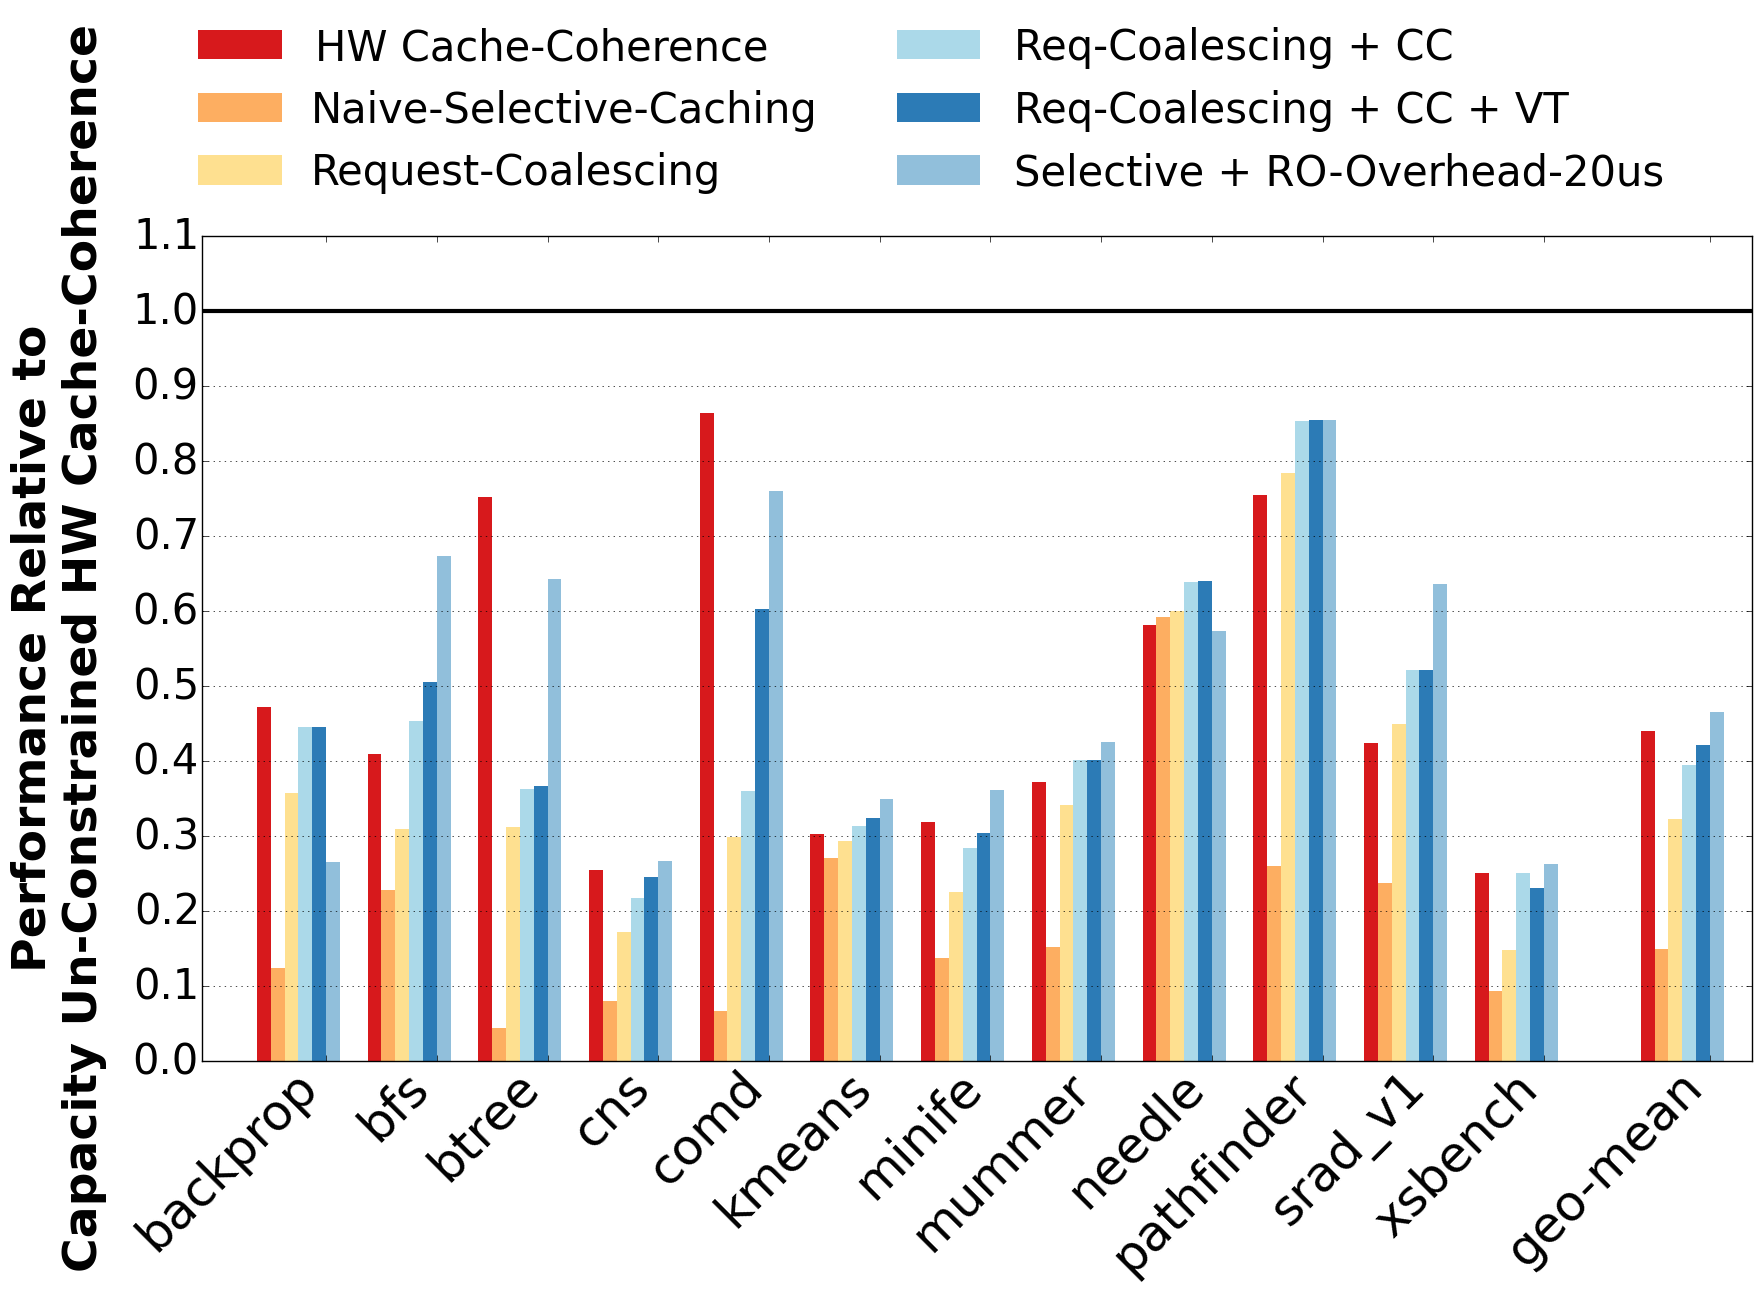
\includegraphics[width=1.0\columnwidth]{hpca2016/figures/capacityconstrained.png}
\caption{GPU performance under memory capacity constraints. (CC: Client-Cache,
VT: Variable-sized Transfer Units)}
\label{fig:capacityconstrained}
\end{figure}

In this work, we have primarily investigated a system where bandwidth-aware page placement
provides an initial page placement that has been shown to have optimal performance~\cite{Agarwal2015}.
Bandwidth-aware page placement is based on the premise that the GPU will place pressure on
the CPU and GPU memory system in proportion to the number of pages placed in each memory.  Proposals,
like selective caching, that change the on-chip caching policy of the GPU can cause dramatic
shifts in the relative pressure placed on each memory system, effectively changing the bandwidth-optimal 
placement ratio.  Although we do not evaluate this phenomenon in this work, balancing
initial page placement with dynamic page migration to help compensate for the lack of on-chip
caching is an area that needs further investigation.

\section{Related Work}
\label{related_work}

Cache coherence for CPUs has received great attention in the literature.
Recent proposals have started to explore intra-GPU and CPU--GPU cache coherence.

\textbf{CPU Systems:} Scalable cache coherence has been studied extensively for CPU-based
 multicore systems. Kelm et al. show that scaling up coherence to hundreds
or thousands of cores will be difficult without moving away from pure
hardware-based coherence~\cite{Kelm2009,Hill92}, due to high directory storage
overheads and coherence traffic~\cite{Lebeck95,Cheng06}.  
Whereas some groups have
evaluated software shared memory implementations~\cite{Falsafi94,Hill92}, Martin
et al. argue that hardware cache coherence for mainstream processors is here to
stay, because shifting away from it simply shifts the burden of correctness into
software instead of hardware~\cite{Martin2012}. Nevertheless, disciplined programming
models coupled with efficient hardware implementations are still being pursued~\cite{choi2011,Sung2013,Sung2015}.

Self-invalidation protocols have been proposed to reduce invalidation traffic and reduce
coherence miss latency~\cite{Lebeck95,Lai2000}. Our cacheless request coalescing scheme uses a similar idea,
discarding a block immediately after fulfilling requests pending at the MSHR.
Other proposals have classified data into private, shared, and
instruction pages and have devised techniques to curtail coherence transactions
for private data~\cite{Pugsley2010,Hardavellas2009,Cuesta2011,Ros2012}. We instead classify
pages into read-only versus read-write and exploit the fact that read-only data
can be safely cached in incoherent caches.

Ros and Kaxiras~\cite{Ros2012} have proposed a
directory\hyp{}less\slash{}broadcast\hyp{}less coherence protocol where all shared
data is self\hyp{}invalidated at synchronization points. In this scheme,
at each synchronization point (e.g., lock acquire/release, memory barrier) all
caches need to be searched for shared lines and those lines have to be
flushed---an expensive operation to implement across hundreds of GPU caches with data
shared across thousands of concurrent threads.

\textbf{Heterogeneous Systems and GPUs:} With the widespread adoption of GPUs as a primary
computing platform, the integration of CPU and GPU systems has
resulted in multiple works assuming that CPUs and GPUs will eventually become
hardware cache-coherent with shared page
tables~\cite{Power2014,Pichai2014,Agarwal2015,Agarwal2015b}.  CPU--GPU coherence
mechanisms have been investigated, revisiting many ideas from distributed shared
memory and coherence verification~\cite{Gelado2010,Power2013,wu2014,Kaxiras2013}. Power et
al.~\cite{Power2013} target a hardware cache-coherent CPU--GPU system by
exploiting the idea of region
coherence~\cite{Cantin2005,Alisafaee2012,Moshovos2005,Zebchuk2007}. They treat the CPU and the
GPU as separate regions and mitigate the effects of coherence traffic by
replacing a standard directory with a region directory. 
In contrast, we identify that CPUs and GPUs need not be cache-coherent; 
the benefits of unified shared memory with correctness guarantees can also be achieved via selective caching, which has lower
implementation complexity.

Mixing incoherent and coherent shared address spaces has been explored before in the context of
CPU-only systems~\cite{Huh04} and the appropriate memory model for mixed
CPU--GPU systems is still up for
debate~\cite{Lim2012,Hechtman2014,Hower2014,Gaster2015}.  Hechtman et al.~propose 
a consistency model for GPUs based on release consistency, which allows
coherence to be enforced only at release operations.  They propose a 
write-through no-write-allocate write-combining cache that tracks dirty data
at byte granularity.  Writes must be flushed (invalidating other cached copies) only 
at release operations.  Under such a consistency model, our selective caching scheme 
can be used to avoid the need to implement hardware support for these invalidations between
the CPU and GPU.

Cache coherence for GPU-only systems has been studied by
Singh et al.~\cite{Singh2013}, where they propose a timestamp-based hardware 
cache-coherence protocol to self-invalidate cache lines. Their scheme targets 
single-chip systems and would require synchronized timers across multiple 
chips when implemented in multi-chip CPU-GPU environments.
Kumar et al.~\cite{Kumar2015} examine CPUs and fixed-function accelerator
coherence, balancing coherence and DMA transfers to prevent data ping-pong.
Suh et al.~\cite{Suh2004} propose integrating different coherence
protocols in separate domains (such as MESI in one domain and MEI in another). 
However, this approach requires invasive changes to
the coherence protocols implemented in both domains and
requires significant implementation effort by both CPU and GPU vendors.

\textbf{Bloom Filters:} Bloom Filters~\cite{Bloom1970} and Cuckoo
Filters~\cite{Pagh2004,fan2014} have been used by several
architects~\cite{Strauss2006,Zebchuk2009,Hongzhou2011} in the past. Fusion
coherence~\cite{wu2014} uses a cuckoo directory to optimize for power and area in
a CMP system. JETTY filters~\cite{Moshovos2001} have been proposed for reducing
the energy spent on snoops in an SMP system. We use a cuckoo filter to implement
the GPU remote directory.


Introducing globally visible shared memory in future CPU/GPU systems
improves programmer productivity and significantly reduces the barrier
to entry of using such systems for many applications. 
Hardware cache coherence can provide such shared memory and
extend the benefits of on-chip caching to all memory within the system.
\ignore{Hardware cache coherence in future CPU/GPU systems would allow the integration
of the separate CPU and GPU programming paradigms under a single
uniform model, leveraging the benefits of on-chip caching for all
memory within the system.}  However, extending hardware cache coherence 
throughout the GPU places enormous
scalability demands on the coherence implementation.  Moreover, integrating
discrete processors, possibly designed by distinct vendors,
into a single coherence protocol is a prohibitive engineering and
verification challenge.  

In this thesis, we demonstrate that CPUs and
GPUs do not need to be hardware cache-coherent to achieve the
simultaneous goals of unified shared memory and high GPU performance.  Our
results show that \textit{selective caching} with request coalescing,
a CPU-side GPU client cache, variable-sized transfer units
can perform within 93\% of a
cache-coherent GPU for applications that do not perform fine
grained CPU--GPU data sharing and synchronization. We also show that promiscuous
read-only caching benefits memory latency sensitive applications using
OS page-protection mechanisms rather than relying on hardware cache coherence.  Selective caching
does not needlessly force hardware cache coherence into the GPU memory system,
allowing decoupled designs that can maximize CPU and GPU performance, while
still maintaining the CPU's traditional view of\ignore{ a hardware coherent} the
memory system.\newpage



% \chapter{Proposal: Thermostat}
% \label{chap:thermostat}
% \section{Introduction}

%%Here is a problem
%Upcoming memory technologies, such as Intel's recently-announced XPoint-3D
%memory, are projected to be denser and cheaper per bit than DRAM while providing
%the byte-addressable load-store interface of conventional main memory.  Improved
%capacity and cost per bit comes at the price of higher access latency, projected
%to fall somewhere in the range of 500ns to several microseconds~\cite{xpoint}.
%The impending commercial availability of such devices has renewed interest in
%two-tiered physical memory, wherein part of a system's physical address space is
%implemented with the slower, cheaper memory technology.  Slow memory can result
%in a net TCO win if the cost savings of replaced DRAM outweigh cost increase due
%to reduced program performance or by enabling a higher peak memory capacity per
%server than is economically viable with DRAM alone.  Our preliminary results
%indicate that over half of the memory footprint of representative cloud
%applications (e.g., Cassandra) are identified as cold by Linux’s kstaled
%mechanism, indicating that the corresponding pages have an inter-access interval
%exceeding 120s.  Analytic modeling suggests these pages could be shifted to a
%memory with a 3us access time with negligible (<3\%) performance degradation.
%
%%It's an interesting problem
%Prior academic work has considered two approaches to two-tiered memory: via a
%paging mechanism~\cite{Ekman2005,Lim2009}, wherein accesses to slow memory
%invoke a page fault that must transfer data to fast memory before an access may
%proceed, and via a migration mechanism (as in cache coherent NUMA
%multiprocessors)~\cite{Lim2009}, wherein no software fault is required.  In the
%latter scenario, a migration mechanism seeks to shuffle pages between tiers to
%maximize fast-memory accesses.  
%
%%It's an unsolved problem
%However, all prior work on two-tiered memory has assumed migration/paging at 4KB
%page granularity.  Huge pages, implemented via Linux's Transparent Huge Page
%(THP) mechanism, are now ubiquitous and critical for cloud applications.
%Recent work~\cite{JeffPaper} has demonstrated that 2MB huge pages are particularly
%performance-critical under virtualization.  For example, our study demonstrates
%a 20\% throughput improvement for Hadoop and a 40\% speedup on random memory
%probes when using huge pages under virtualization.  Huge pages thwart prior
%two-tiered memory proposals for two reasons: (1) it is too expensive to
%frequently migrate pages at 2MB granularity, and (2) hot regions occur within
%otherwise cold 2MB huge pages. 
%
\begin{figure}[t]
\centering
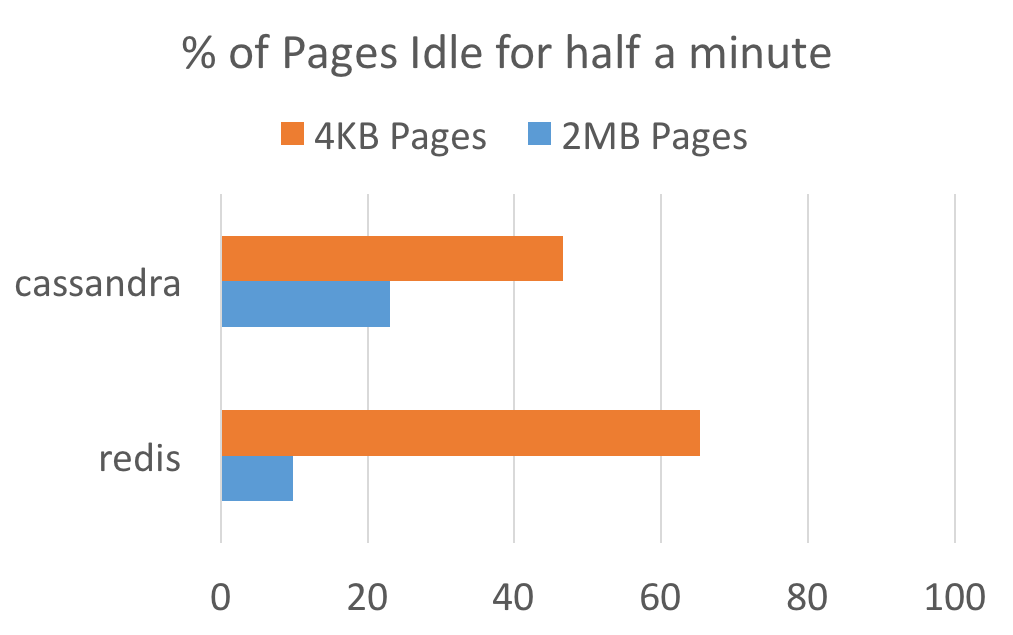
\includegraphics[width=1.0\columnwidth]{thermostat/figures/cold-data.png}
\caption{Amount of cold data in applications, thp vs no-thp numbers}
\vspace{-0.175in}
\label{fig:motivation-thermostat}
\end{figure}

%%Here is my idea
%Our Proposal: We propose to develop a transparent huge-page-aware two-tiered
%memory solution that integrates support for dynamic page migration and
%transparene huge pages, achieving both the capacity/cost advantages of
%two-tiered memory and performance advantages of huge pages.  Our focus is on
%cloud computing scenarios where a high-memory-footprint application, such as
%Cassandra, Aerospike, or MySQL, runs under virtualization and may co-run with
%other, competing applications.
%
%Hot regions within otherwise cold huge pages present a central challenge to our
%objective; existing x86-Linux provides no mechanism to carve out a 4KB hot
%region within a 2MB cold page.  So, we propose translation facades, a 4KB
%translation that remaps a portion of a 2MB mapping with an alternate physical
%address or permissions.  Current x86-Linux requires non-overlapping mappings due
%to hard-coded page table structure and because TLB entries are replaced
%independently, hence, an uncached 4KB facade to a cached 2MB translation could
%lead to a mis-translation. We will pursue implementations of translation
%facades along two paths. (1) Hardware support: we will extend x86 page table and
%TLB design to support facades. (2) Virtualization: Our existing study of huge
%pages under virtualization demonstrate that a majority of the benefit can be
%obtained if host pages are 2MB even if guest pages are 4KB.  We will investigate
%if the two-level translation from guest to host to machine addresses can be
%exploited to emulate hardware support for translation facades.
%
%%Bulleted list of contributions
%Our research program will follow a four-fold approach.  (1) We will measure hot
%and cold memory fractions at 4KB granularity and within 2MB huge pages to
%measure two-tiered memory opportunity and demonstrate the need for translation
%facades. We will use kstaled (an optional extension to the Linux kernel that
%tracks pages that have not been accessed over a fixed time interval) and
%BadgerTrap [4] (a tool to intercept soft page faults) to facilitate this
%characterization. (2) We will develop methods to track hot and cold memory
%regions at run-time.  A key challenge lies in efficiently tracking hot regions
%within an otherwise-cold huge page, as kstaled provides visibility only at page
%granularity.  We propose to investigate sampling methods, e.g., by
%probabilistically demoting huge pages or leveraging performance counter
%infrastructure. (3) We will develop an online migration mechanism that can shift
%data between fast and slow memory tiers while the application is concurrently
%executing. We draw experience from existing NUMA migration and THP memory
%defragmentation. We will implement the migration mechanism in the Linux kernel.
%(4) We will develop translation facades (using BadgerTrap to emulate
%performance) and investigate novel page table and TLB organizations to support
%facades.

%TODO My idea works
%TODO Here's how my idea compares to other people's approaches

%OLD TEXT
%
Upcoming memory technologies such as Intel 3D-XPoint~\cite{xpoint} are an
attractive candidate for reducing main memory costs (both in terms of CapEx and
OpEx) in data-centers, which is pegged at 30\% of TCO by recent
estimates. Such memory technologies have two defining characteristics
that set them apart from commodity DRAMs: a) they are much cheaper per unit
capacity than DRAM, with current estimates putting them at $50\%$ cheaper
than DRAM, and, b) they are much slower than DRAM technology. Whereas
commodity DDR3/DDR4 has a latency of $\approx$100ns, such upcoming memory
technologies have latencies of the order of 400ns--1us.

Because of such high access latencies of newer memory technologies, they can not
completely substitute DRAMs. Instead, a prime area for such technologies is for
storing {\it cold} data of applications.  Our preliminary results shown in
Figure~/ref{fig:motivation} indicate that over half of the memory footprint of
representative cloud applications (e.g., Cassandra) are identified as cold by
Linux’s kstaled mechanism, indicating that the corresponding pages have an
inter-access interval exceeding 120s.  Analytic modeling suggests these pages
could be shifted to a memory with a 3us access time with negligible ($<$ 3\%)
performance degradation.

%It has been shown
%that a major fraction (XXX\% by some estimates~\cite{XXX}) of application
%footprint in current cloud/datacenter workloads is {\it cold}, i.e., rarely
%touched by the application. 

Placing such data in slow memories does not degrade the application throughput
or latency significantly, while also reducing the amount of costly DRAM required
in data-centers by a significant margin. In order to perform such placement in a
application-transparent fashion, the identification of cold data is done at an
OS page granularity, where a page is deemed to be a ``hot page'' if any of the
data present in that page is hot.

As a consequence of this mechanism, when going to larger page sizes (2MB/1GB
instead of the currently prevailing 4KB), a significantly smaller fraction of
pages is classified as ``cold''. This is because the presence of even a {\it
single} hot data item in an otherwise cold page will result in the entire page
being classified as hot. Using a smaller page size could have identified the
locations of the hot data more precisely, and thereby resulted in a larger
fraction of cold pages. Such a ``hotSpot'' distribution of hot data is common in
data-center applications, and according to our estimates, using 2MB sized pages
reduces the fraction of cold pages by $\approx$2-3$\times$. Thus, using larger
page sizes cause sub-optimal usage of cheap memory technologies in data-centers.

However, usage of large page sizes, typically done in Linux through {\it
Transparent Huge Pages (THP)}, is ubiquitous in modern data-center applications.
THP is a mechanism available in the Linux kernel whereby applications can
transparently use large (2MB) or huge (1GB) sized pages without any source code
change. Larger page sizes has been shown to reduce page faults and thereby
improve throughput and latency in data-center applications significantly. Our
studies demonstrate that 2MB huge pages are particularly
performance-critical under virtualization.  For example, we observe 
a 20\% throughput improvement for Hadoop and a 40\% speedup on random memory
probes when using huge pages under virtualization.  However, huge pages pose two
challenges to prior two-tiered memory proposal: (1) migrating pages at 2MB
granularity is expensive, and (2) hot regions occur within otherwise cold 2MB
pages, which if placed in slow memory can hurt application service level
agreements (SLAs) making cheaper slower new memory technology unemployable at
scale.
%Thus, most of such applications are currently run with THP, and
%turning off THP is not a viable solution in most-if-not-all cases. Thus, there
%is a dilemma between choosing THP, thereby benefiting from the large
%application speedups, and not choosing THP, thereby lowering data-center memory TCO by
%placing larger fractions of application footprint in cheap memories.

We propose translation facades, a 4KB translation that remaps a portion of a 2MB
mapping with an alternate physical address or permissions.  Current x86-Linux
requires non-overlapping mappings due to hard-coded page table structure and
because TLB entries are replaced independently, hence, an uncached 4KB facade to
a cached 2MB translation could lead to a mis-translation. We will pursue
implementations of translation facades along two paths. (1) Hardware support: we
will extend x86 page table and TLB design to support facades. (2)
Virtualization:
%Our existing study of huge pages under virtualization
%demonstrate that a majority of the benefit can be obtained if host pages are 2MB
%even if guest pages are 4KB.
We will investigate if the two-level translation
from guest to host to machine addresses can be exploited to emulate hardware
support for translation facades.

%}).\section{Background and Motivation}
%\label{motivation}
%
%\begin{figure}[t]
%\centering
%\includegraphics[width=1.0\columnwidth]{thermostat/figures/hotspot-cdf.png}
%\caption{HotSpot huge page distribution}
%\vspace{-0.175in}
%\label{fig:hotspot-cdf}
%\end{figure}
%
%Cold data at 4KB granularity vs 2MB granularity. Use figure to show quantify
%HotSpot pages within an otherwise cold huge page.
%
%Show analytical analysis of putting pages in slow memory and opportunity to make
%slow memory usable in data centers.
%
%Discuss performance-cost trade-off for data centers.
%
%Why are previous 2-level memory techniques inadeqaute in solving this issue.
%
%Re-iterate the problem we are solving and the central idea of our solution.
%
\section{Background}
\subsection{Virtual Memory Management}
\begin{figure}[t]
\centering
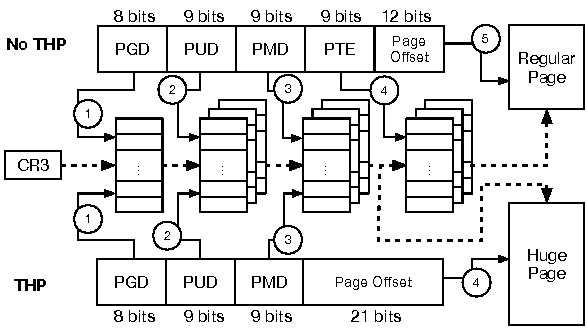
\includegraphics[width=0.45\textwidth]{thermostat/figures/linux_pgtable.pdf}
\caption{
Linux page table structure for X86 both with and without a transparent huge page.
}
\label{fig:linuxpgtable}
\end{figure}


As the size of main memory has grown, the overheads of virtual memory systems
have grown as well.  The hierarchical Linux page table for the x86-64
architecture, shown in Figure~\ref{fig:linuxpgtable}, addresses up to 128 terabytes of
memory and is four levels---and thus may incur up to four extra memory
operations to perform a single translation \cite{pgtable}.
%\fixme{This text is a candidate to cut to save space: Translation begins with
%the page global directory (PGD), pointed to by the CR3 register, which is
%preloaded with the PGD base address upon a context switch.  Bits 39-46 of the
%virtual address are used to index the PGD, yielding a page upper directory
%(PUD) structure, which is subsequently indexed by bits 30-38 of the virtual
%address to produce a page middle directory (PMD) structure.  When the
%translation target lies on a physical page of the 4 KB base page size (shown on
%the top in \pref{fig:linuxpgtable}), the PMD is indexed with bits 21-29, giving
%a page table entry (PTE) that is indexed by bits 12-20 to finally generate a
%physical page number.  Throughout this process, as many as four extra memory
%operations may be performed purely as an overhead of the virtual memory
%translation system.}
Moreover, execution in virtualized environments can sextuple translation costs
\cite{amdnested,intelept,bhargava:2008:atp}.  As a result, the Translation
Lookaside Buffer (TLB), which acts as a cache for virtual-to-physical mappings,
has become increasingly important to mollify the effects of virtual memory
translation overhead.

In most architectures, TLB accesses lie on the critical path of memory accesses,
hence hardware timing constraints limit the number of TLB entries that can be
searched on each access.  As memory capacities grow while page sizes remain
constant, TLB coverage---the portion of main memory that can be represented by
the contents of the TLB at any given time---necessarily decreases.  This reduced
coverage hampers the performance of programs with large working sets and/or
instruction footprints because it increases the number of TLB misses they
exhibit, and thus the number of page table walks that must be performed.  What's
more, as working set sizes---and, correspondingly, page table sizes---grow, the
fraction of translation data that can fit in the cache is reduced, leading to
more severe TLB miss penalties.

Recognizing the high cost of TLB misses in cloud applications, a number of
recent research efforts have sought hardware solutions to mitigate their penalty
(e.g., \cite{bhattacharjee:2011:slt, srikantaiah:2010:sth, barr:2011:sms,
pham:2012:ccl, basu:2013:evm, gandhi:2014:emv}.
Whereas these techniques reduce or hide TLB miss stalls, they do not address the
cost of managing numerous page tables entries or the cache capacity occupied by
them.

%One line of work seeks architectural solutions to improve the reach of TLBs,
%for example, through 2-level TLBs .  These mechanisms can improve TLB hit
%rates, but require hardware changes and do not address the cost of managing
%page tables, which manifest during a variety of system calls (e.g., upon
%allocations, faults to access \texttt{mmap()}'d files, and forks).  A second
%line of work revisits alternative memory virtualization schemes, such as
%segmentation, in the context of modern systems \cite{basu:2013:evm,
%gandhi:2014:emv}.  While new hardware support for segmentation may address TLB
%capacity limitations for the user heap, it does not provide a straightforward
%solution for OS structures that may require finer-grained protection, such as
%the file system page cache.

Huge pages directly address the costs of fine-grain page management.
%They require hardware support in the TLB for huge-page entries (either
%dedicated entries or support for multiple-sized lookups), but this support is
%ubiquitous in existing architectures (e.g., Intel's Haswell processor
%provisions 32 entries for huge pages in its L1 data TLBs).
They effectively increase TLB coverage---one huge page TLB entry covers the area
of a large number of regular page entries---thus reducing page faults, and they
reduce the size of the page table structure, leading to both fewer memory
accesses upon a TLB miss and increased cache-ability of translation data.
%on a TLB miss they can reduce the number of page table accesses necessary to
%resolve a virtual-to-physical mapping.  The latter arises due to the fact that
%a huge page covers a much larger range of virtual memory.
%\pref{fig:ahppgtable} displays the most efficient possible hierarchical page
%table topology for x86-64 Linux if it is backed by 2MB huge pages.
%In contrast to the page table shown in \pref{fig:linuxpgtable}, this structure
%requires only two extra memory accesses due to the increased coverage at each
%level.  Though TLB support for huge pages is ubiquitous in existing
%architectures (e.g., Intel's Haswell processor TLBs provision 32 entries for
%huge pages in the L1 data TLB), unfortunately the current x86-64 architecture
%specifies the page table layouts shown in \pref{fig:linuxpgtable}.
%and precludes a design like that in \pref{fig:ahppgtable}.
%We hope our results might motivate greater flexibility in future architecture
%revisions.
%
%\input{fig.ahppgtable}

\subsection{Background: Transparent Huge Pages} \label{sec:thp_bg}
%\fixme{This paragraph strongly duplicates the intro.  We should say this in
%only one place.  My suggestion is to cut down the intro and leave the details
%here. --- Jeff: fixed}
Early system support for huge pages, static huge pages, requires bucketing the
available physical memory at boot time into standard pages and huge pages.
Static huge pages are disjoint from the standard memory pool and cannot be used
for the disk page cache, disk write buffers, or any kernel data structure.
Moreover static huge pages require application changes and are thus
non-transparent to the programmer. The static provisioning of memory into static
huge pages also leads to allocation problems and memory stranding if the actual
demand for huge pages does not match the boot-time configuration.  Thus, even if
applications are static huge page-aware, such a solution is less than ideal for
many systems because it requires a priori knowledge of applications' memory
requirements to ensure ideal performance.

Recent versions of the Linux kernel instead exploit huge pages through THP.
With THP, the kernel attempts to invisibly (i.e., without the knowledge of the
user) allocate huge pages to back large regions of contiguous virtual memory.
Transparent allocation is advantageous because it allows existing codebases to
reap the rewards of huge pages without modification and doesn't require changing
the interfaces and invariants of system calls and functions that require
consideration of page size, such as \texttt{mmap()}.  However, the kernel may
demote allocated huge pages by breaking them down into a set of regular pages
when it deems necessary  to maintain support for functions that are not huge
page-aware.

\textbf{Allocation/Promotion:} The first time an application touches an
allocated region of virtual memory, a page fault occurs and the kernel allocates
one or more physical pages to back that region and records the virtual to
physical mapping.  With THP enabled, the kernel allocates huge pages for
anonymous (i.e., non-file-backed) regions of huge page-sized and -aligned
virtually contiguous memory during the initial page fault to that region.
%Alternatively, if a huge page isn't initially available or the size and
%alignment requirements are not met, a region of virtual memory that isn't
%initially backed by huge pages can later be promoted if the virtual region is
%later modified to meet these requirements.  In the process of promotion, the
%regular page-backed virtual region is collapsed into a huge page-backed region,
%thus multiple regular pages are marked to be treated as a single huge page.
Alternatively, if a region isn't initially backed by a huge page, it can later
undergo promotion, in which multiple regular pages are marked to be treated as a
single huge page.  The kernel can be set to either aggressively allocate huge
pages whenever it can, or to only allocate them when the user provides hints via
the \texttt{madvise()} system call.

\textbf{Demotion:} Any region backed by a huge page may be subject to
spontaneous demotion to regular pages.  Because various parts of the kernel
source code are not huge page-aware, giving them access to a huge page could
lead to unspecified or erroneous behavior.  As a result, huge pages are often
\emph{split}, or broken into several regular pages, before they are passed to
functions that are not huge page-aware.  To perform this split, the page table
must be updated to reflect the many regular pages that comprise the demoted huge
page.

%Another notable characteristic of THP is that it does not increase the coverage
%of the various levels of the page table (due to architectural constraints
%described in \pref{sec:limitations}).  Therefore, while the physical page size
%is increased, the coverage of each level of the page table remains the same.
%The translation procedure for \thp, shown on the bottom in
%\pref{fig:linuxpgtable}, elides the PMD$\to$PTE step necessary with regular
%pages and produces a physical page number at the PMD level.
%
%In contrast to the two memory access translation shown in
%\pref{fig:ahppgtable}, a \thp translation requires three accesses.
%
%\subsection{Pathologies of THP} \label{sec:thp_problems}
%
%\input{fig.frag_bench.tex}
%
%Though \thp has the potential to improve average application throughput, it can
%negatively impact latency and performance isolation between unrelated
%applications.  A widely known effect of paged virtual memory is external memory
%fragmentation---small blocks of free memory separated by large blocks of
%allocated memory.  With \thp, a system exhibiting significant memory
%fragmentation may not always have huge page-sized regions of contiguous
%physical memory available for allocation, even if much of memory is free.
%
%Severe memory fragmentation is particularly common in cloud computing
%workloads, where processes start and end frequently.  In systems with few,
%long-lived processes, virtual memory rarely becomes fragmented---most user-mode
%allocators do not frequently return freed memory to the operating system,
%instead retaining and managing it in pools.  In contrast, many cloud
%environments collocate multiple processes that start and end frequently in a
%single machine.  For example, map-reduce clusters execute thousands of
%processes that may each last only minutes.  Main memory will rapidly fragment
%due to the varying allocation sizes of these numerous short-lived processes.
%I/O intensive workloads can also cause rapid memory fragmentation due to random
%access I/O populating the page cache with many small allocations, which are
%subsequently reclaimed without regard to layout.
%
%When a huge page is requested during a page fault but cannot be served, the
%Linux memory manager has two options: it can either turn down the request and
%fall back on regular pages to serve the fault, or it can stall the program and
%defragment memory to create a huge page-sized chunk to allocate.  The former
%option is not ideal, as it prevents applications from reaping the benefits of
%huge pages when there is still enough physical memory available to accommodate
%them.  However, the performance cost of synchronous (\ie, blocking)
%defragmentation can be significant, as execution of the application must be
%paused while the kernel migrates regular pages to make room for a huge page.
%
%While defragmentation is in progress, the kernel will obtain and hold locks
%that can block progress of other applications that happen to concurrently
%request memory.  Hence, defragmentation impacts not only the application
%requesting the huge page, it can also result in stalls in ``innocent
%bystander'' applications.  Indeed, in our experience, a pathological behavior
%in defragmentation code triggered by one application caused multi-millisecond
%(and initially unexplainable) latency spikes in an unrelated production service
%that happened to collocate on the same server.  The kernel locks held by
%defragmentation code caused allocation delays to spread virally among
%applications.  These THP pathologies have been documented by others as well
%\cite{zhuang:2014:ehm, rientjes:2014:email, oracle:2013:blog, rahn:2012:blog}.
%Whereas some of these issues have been mitigated (after several man-months of
%investigation), these pathologies motivated this study of the \thp mechanism,
%and prompted us to ask whether, perhaps, the entire mechanism should be
%discarded.
%
%To our dismay, one such pathology in \thp can be triggered in recent versions
%of the kernel (in which the behavior is ostensibly fixed), even without exotic
%application behaviors.  To reconstruct this behavior, we use a memory
%allocation microbenchmark that measures the latency of allocation (\ie, time
%needed for the kernel to find and map a physical page) for 2MB regions
%allocated on the heap using unmodified GLIBC \texttt{malloc()}.
%\pref{fig:frag_bench} shows the impact of synchronous memory defragmentation on
%allocation tail latency in a virtual machine running version 3.13 of the Linux
%kernel.
%% when using only \texttt{malloc()} to fragment memory, as might naturally arise after running map-reduce processes for several hours. %
%%We measure a memory allocation microbenchmark, which allocates and initializes huge page-sized chunks of memory using unmodified GLIBC \texttt{malloc()}, causing the kernel to attempt to allocate huge pages when the THP mechanism is enabled.
%We report the cumulative distribution of the latency of individual allocations
%(note the logarithmic x-axis scale).  We consider four scenarios, two with \thp
%enabled and two with it disabled.  We consider scenarios where memory is
%initially unfragmented (all memory is free and the page cache is empty) and
%where it has been aggressively fragmented.  We fragment memory using a large
%number of processes that repeatedly allocate and free memory chunks of random
%sizes---a scenario representative of a series of map-reduce tasks.  These
%processes are continually spawned and killed (to return their allocated memory
%to the kernel), with the last set of processes ultimately holding a final set
%of allocations (partially filling memory) and quiescing.  Further details of
%our test setup appear in \pref{sec:methodology}. %\fixme{Confirm that we
%actually do provide further details in the results section.}
%
%There are two key take-aways from this experiment.  First, \thp substantially
%reduces latency for most allocations.  Median allocation latency is reduced
%from about 700us to about 500us.  Allocations become faster on average because
%the kernel must create and map far fewer PTEs (by as much as a factor of 512)
%for large allocations.  When memory is unfragmented, nearly all allocations are
%faster under \thp.  In contrast, when memory is fragmented, synchronous
%compaction severely delays a significant fraction of allocations, in some cases
%increasing latency by orders of magnitude.  About 20\% of allocation requests
%take longer than 1ms with allocations in the 99th percentile taking over 100ms.
%
%Though the tail latency of memory allocation under such circumstances isn't
%critical in all applications, especially those with steady-state heap activity,
%it can have negative effects on other tail-latency-sensitive workloads.
%Workloads such as web search, for instance, perform significant fan-out and
%fan-in operations, where stragglers impact overall latency
%\cite{dean:2013:tas}.  For such applications, unpredictable allocation tail
%latency or stalls of bystander applications/threads can severely impact
%application service level objectives.
%
%One alternative to avoid this unpredictability is to asynchronously (\ie, on
%idle cores) defragment memory to help alleviate the amount of defragmentation
%that must be done at allocation time.  This feature is available in the Linux
%kernel, but it comes with a tradeoff: setting the defragmentation daemon to be
%too aggressive causes it to consume substantial CPU time, harming the
%performance of other threads (and reducing the throughput benefit of \thp)
%\cite{zhuang:2014:ehm}, but setting it to be too passive results in little net
%benefit.  We examine this trade-off in \pref{sec:case_study}.  Alternatively,
%one might reduce the aggressiveness of or disable synchronous compaction
%altogether.  However, doing so often precludes huge page allocation, resulting
%in a performance loss in the common cases where synchronous defragmentation
%does not dominate allocation time.  Thus, supporting multiple pages sizes leads
%to a catch-22; aggressive compaction leads to performance loss due to invasive
%use of system resources, and less aggressive or no compaction results in
%performance loss because huge pages cannot always be allocated on-demand.  As a
%result, THP---or any system that supports multiple page sizes---is inherently
%disadvantaged when large chunks of memory are scarce, as when the system is
%under heavy memory pressure or subject to external fragmentation.
%%
%%under memory pressure or fragmentation.

\section{Thermostat Design}
\label{proposal}
We propose to explore and develop an end-to-end Linux Prototype supported with
minimal hardware changes to employ slower but cheaper memory technologies in
data-centers providing higher capacity at lower cost of ownership.

\subsection{Identifying HotSpots in Cold Hugepages}

%\begin{figure}[t]
%\centering
%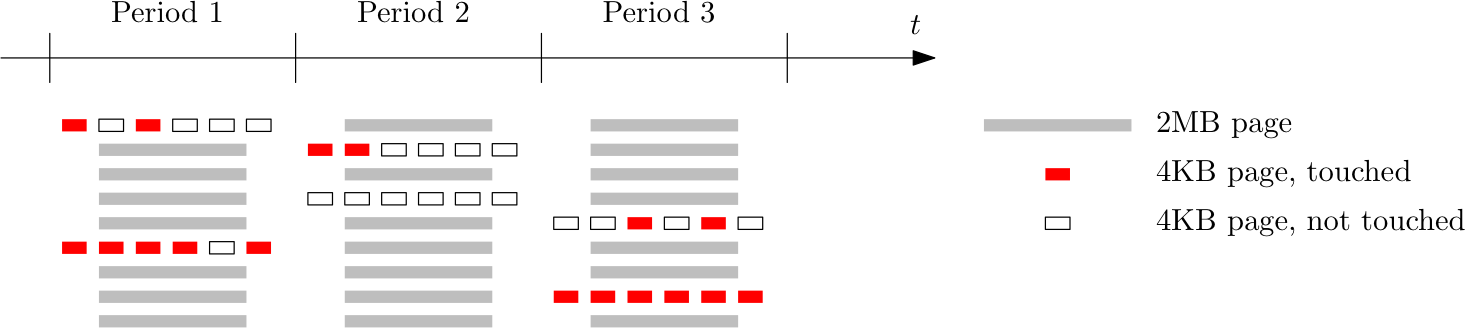
\includegraphics[width=1.0\columnwidth]{thermostat/figures/sampling.png}
%\caption{Sampling to identify HotSpot pages in otherwise cold page}
%\vspace{-0.175in}
%\label{fig:sampling}
%\end{figure}
To solve this situation, we propose to build a dynamic controller (which we call
Thermostat) that can decide when to {\it break} a huge page into several regular
pages, and place some of those smaller pages which are deemed to be cold in
slower but cheaper memory. We will implement Thermostat as a part of custom
Linux prototype.

The Thermostat controller has to distinguish between ``hotSpot'' hot pages --
ones with only a few hot data blocks, and ``uniform'' hot pages -- ones where a
significant fraction of the data blocks in that page are hot.  We propose to
build such a classification mechanism that is at once a)
application-transparent, i.e., no source code change in the application should
be necessary, b) low-overhead, so as to not degrade the performance benefits of
using THP, and, c) high-accuracy, i.e., most of the classified ``hotSpot'' pages
are indeed hotspots (low false positives) and most of the pages classified
``uniform'' are {\it} not in fact hotspots (low false negatives).

We observe that there are hot 4KB pages present within 2MB huge pages.
Figure~\ref{fig:motivation-thermostat} shows that applications on average have
$\approx$ 50\% of cold data. As we change page size form 4KB to 2MB fraction of
cold data reduced by $\approx$ 20\%. Page granularity based OS mechanisms cannot
reveal the hot portions within huge pages. Hence, we propose a sampling based
page temperature measurement mechanism that classifies pages by their access
rate.

%
%\begin{figure}[t]
%\centering
%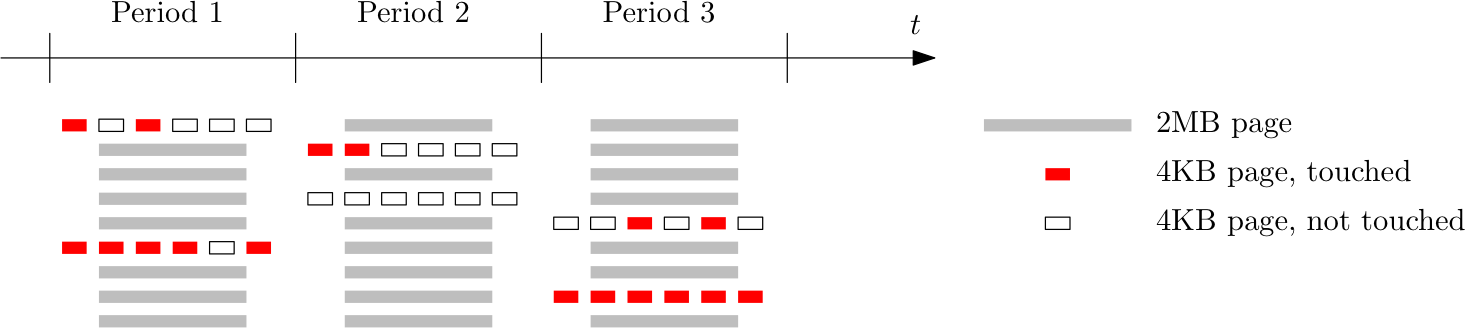
\includegraphics[width=1.0\columnwidth]{thermostat/figures/sampling.png}
%\caption{TLB and PTE changes}
%\vspace{-0.175in}
%\label{fig:motivation}
%\end{figure}
%
%\subsection{Sampling Mechanism}
%The Thermostat controller needs an effective mechanism for chunking up a DRAM
%huge page into several small pages, and also for compacting several small hot
%pages into a single DRAM huge page. Chunking up a huge page is relatively simple
%-- one need only allocate several page table entries (PTEs) corresponding to the
%chunked up page. Doing the inverse, that is compacting several small pages from
%the slow-mem and DRAM into a single DRAM huge page has more challenges. First,
%due to memory fragmentation, it may not be possible to find a suitable space to
%put the newly created huge page. Second, reading several small pages from
%slow-mem, and creating a huge page out of them can be a potentially very long
%latency operation, which can then affect application throughput as well as tail
%latency. We plan to study the design trade-off space of when to perform
%these operations and incorporate the obtained insights into building the Thermostat
%controller.
\subsection{Translation Facades}
Thermostat will divide application pages into categories: (1) Extremely hot huge
pages -- pages with high access rates, (2) Extremely cold huge pages -- pages
with low access rates, and (3) ``hotSpot'' huge pages -- cold 2MB page with
certain 4KB hot regions. We will put extremely hot huge pages in fast memory and
extremely cold huge pages in slow memory. However, there are following
challenges in placing {\it hotSpot} huge pages in either of the fast memory or
slow memory technology: (1) placing them in slow memory can hurt performance due
to high access rates to 4KB hots spots in otherwise cold 2MB page, and (2)
placing them in DRAM will lead to in-efficient utilization of slow and cheaper
memory capacity.
%Another option is to break such {\it hotSpot} huge pages into
%regular pages and place hot 4KB pages in DRAM and cold 4KB pages in slow memory,
%but breaking such huge pages can potentially lead to loosing performance
%benefits of huge pages. In Redis we observe that there is a large fraction of
%{\it hotSpot} huge pages with more than 15\% of 4KB pages wihtin 2MB pages being
%hot. Hence, none of the above techniques can fully exploit the potential savings
%of placing large fraction of pages in cheaper slow memory, while still reaping
%the performance benefits of THP.
%
%Therefore, we propose ``translation facades'', a mechanism that remaps a portion
%of a 2MB mapping with alternate physical addresses or permissions at 4KB
%granularity. HotSpot pages will have multiple valid mappings, hot regions with
%valid 4KB mapping and cold regions with valid 2MB mapping. We propose to modify TLB
%and page table structures to support such multiple mappings.

As a solution to both these problems, we plan to experiment the following two
approaches. The first approach is to break such {\it hotSpot} huge pages into
regular pages and place hot 4KB pages in DRAM and cold 4KB pages in slow memory.
A significant upside of such an approach is that it can be implemented without
any significant hardware changes. However, breaking such huge pages can
potentially lead to losing performance benefits of huge pages. For example, in
Redis we observe that there is a large fraction of {\it hotSpot} huge pages ($>$
30\% of total pages).

As a second approach, we propose ``translation facades'', a mechanism that
remaps a portion of a 2MB mapping with alternate physical addresses at 4KB
granularity. HotSpot pages will have multiple valid mappings, hot regions with
valid 4KB mappings and cold regions with a single valid 2MB mapping. We propose
to modify TLB and page table structures to support such multiple mappings.

%\section{Methodology}
\label{methodology}

\subsection{System Configuration}
Linux 3.16 with changes.
Machine Configuration
\subsection{Cold page identification: kstaled}
Describe how kstaled works. Reference kstaled patches.

\subsection{Emulating slow memory in software: BadgerTrap}
Short description of badger trap and how we modified it to simulate slow memory
and also sample hot portions in cold pages

\subsubsection{overhead of BadgerTrap}

\subsection{HotSpot huge page identification: Sampling Overhead}

%\section{Results}
\label{results}

\subsection{Thermostat Performance Evaluation}
All-DRAM with 4KB\\
All-DRAM with THP\\
2-level memory at 4KB with kstaled doing page placement\\
2-level memory with THP with kstaled doing page placement\\ 
2-level memory with our design\\

\subsection{DRAM Cost Analysis}

Once the Thermostat controller has been built, we propose to perform the
following experiments. First, we will study the impact on application
performance of employing slow-mem on several cloud-computing
applications~\cite{Perfkitbenchmarker}. Satisfying SLAs is compulsory for these
applications as it directly impacts businesses they are deployed in. We will
design our mechanism so that SLAs are not violated in all of these benchmarks.

Second, we will perform a sensitivity study of different policies that Thermostat
controller employs and estimate the corresponding TCO savings. The goal of
employing Thermostat controller is to reduce main memory TCO. However, Thermostat is
expected to increase the CPU usage as well, which will add to the TCO cost. We
will investigate this trade-off of plausible main memory TCO reduction and extra
CPU usage cost.

Finally, we will do a trade-off analysis of performance and TCO with Thermostat.
Looking at only performance (throughput or latency) or TCO can lead one to wrong
conclusions. We will analyze all possible potential impacts of Thermostat on TCO,
including, e.g., cost and power consumption of new memory technologies, power
consumption of Thermostat controller on CPU, additional provisioning that may be
necessary because of lower throughput at SLA etc. One of our end goals is
to come up with a detailed analysis of when using such memory technologies can
be beneficial and drive the adoption of such technologies by internet giants.

\subsection{Discussion}
Varibale that this design will influence in other parts of the system, CPU,
power analysis

%\section{Related Work}
\label{related}

Using NVM as filesystem~\cite{nvm:filesystem:lwn}.

%\section{Conclusion}
\label{conclusion}



 \chapter{Thermostat: Application-transparent Page Management for Two-tiered
Main Memory}
 \label{chap:thermostat}
 %\begin{abstract}
\vspace{0.05in}
The advent of new memory technologies that are denser and cheaper than commodity
DRAM has renewed interest in two-tiered main memory schemes.  Infrequently
accessed application data can be stored in such memories to achieve significant
memory cost savings.  Past research on two-tiered main memory has assumed a 4KB
page size.  However, 2MB huge pages are performance critical in cloud
applications with large memory footprints, especially in virtualized cloud
environments, where nested paging drastically increases the cost of 4KB page
management.  We present Thermostat, an application-transparent huge-page-aware
mechanism to place pages in a dual-technology hybrid memory system while
achieving both the cost advantages of two-tiered memory and performance
advantages of transparent huge pages.  
We present an online page classification mechanism that accurately
classifies both 4KB and 2MB pages as hot or cold while incurring no
observable performance overhead across several representative cloud
applications.
We implement Thermostat in Linux kernel version 4.5 and evaluate its effectiveness on
representative cloud computing workloads running under KVM virtualization.  
We emulate slow memory with performance characteristics approximating
near-future high-density memory technology and show that Thermostat
migrates up to 50\% of application footprint to slow memory while limiting performance
degradation to 3\%, thereby reducing memory cost up to 30\%.
\end{abstract}

\section{Introduction}
\label{asplos2017-introduction}

\begin{figure}[t]
\centering
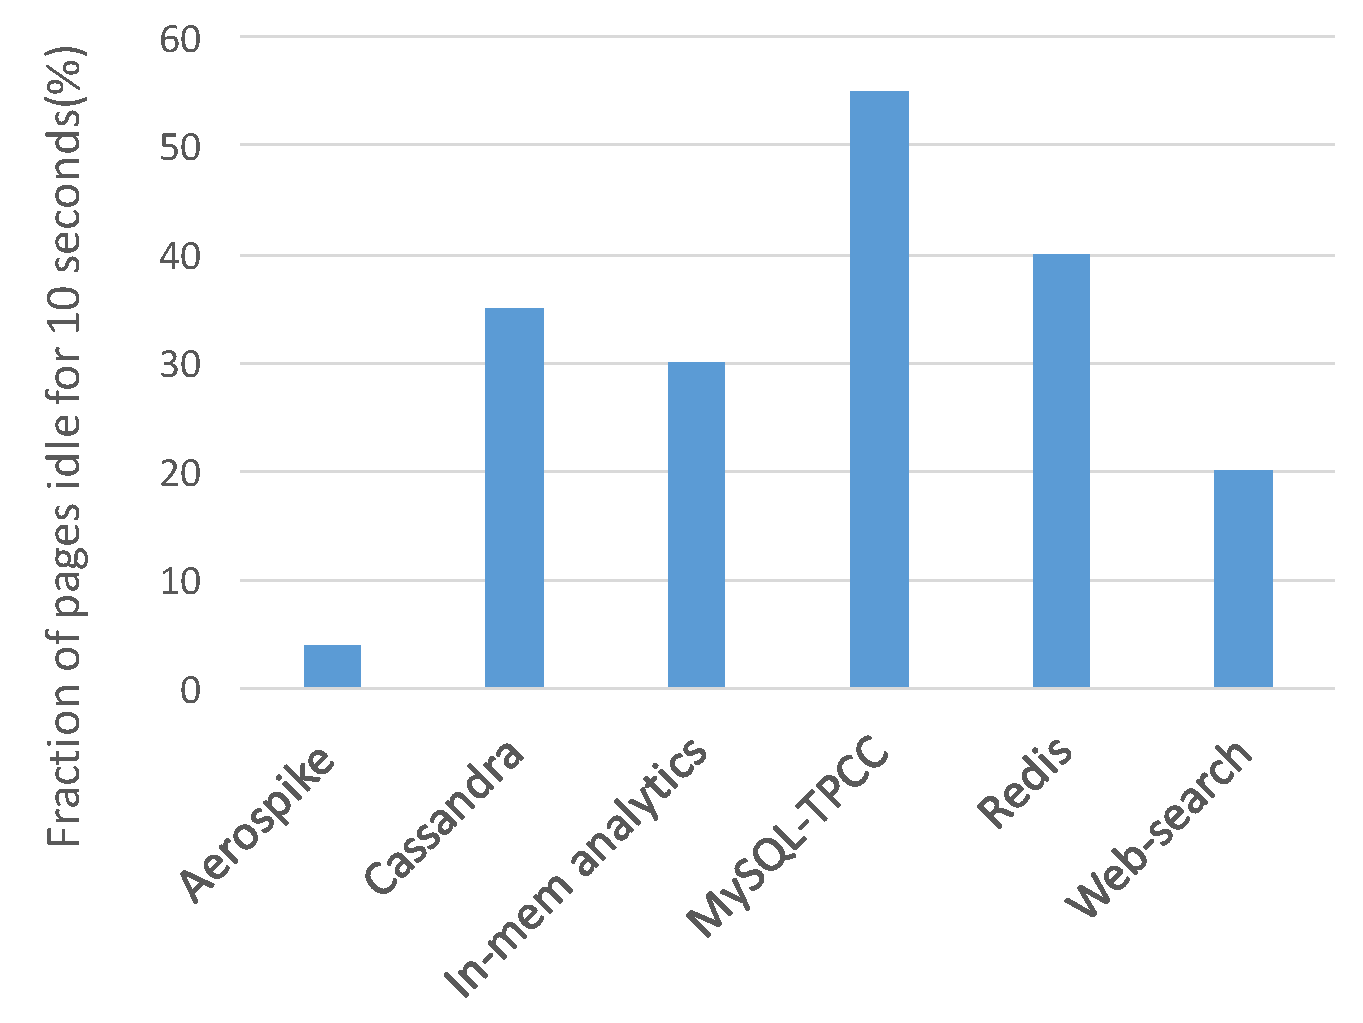
\includegraphics[width=1.0\columnwidth]{asplos2017/figures/kstaled-cold-data-10s}
\caption{Fraction of 2MB pages idle/cold for 10s detected via per-page {\it Accessed} bits
in hardware. Note that this technique cannot estimate the page access rate, and
thus cannot estimate the performance degradation caused by placing
these pages in slow memory (which exceeds 10\% for Redis).}
\label{fig:motivation}
%\vspace{-0.225in}
\end{figure}


%Here is a problem
Upcoming memory technologies, such as Intel/Micron's recently-announced 3D XPoint
memory~\cite{3dcrosspoint}, are projected to be denser and cheaper per bit than DRAM while
providing the byte-addressable load-store interface of conventional main memory.
Improved capacity and cost per bit come at the price of higher access latency,
projected to fall somewhere in the range of 400ns to several
microseconds~\cite{3dcrosspoint} as opposed to 50--100ns for DRAM. The impending commercial availability of such
devices has renewed interest in two-tiered physical memory, wherein part of a
system's physical address space is implemented with the slower, cheaper memory
technology~\cite{ref:Dulloor:datatiering,qureshi:twolm}.  

Slow memory can result in a net cost win if the cost savings of
replaced DRAM outweigh cost increase due to reduced program performance or by
enabling a higher peak memory capacity per server than is economically viable
with DRAM alone. 
%For a 50\% occupied data center the capital expenditure is estimated to be 17\%\cite{borosso2013}. 
%If we assume that slow memory is 3\texttimes~cheaper (per GB) than DRAM 
%and that main memory comprises 30\% of server cost~\cite{borosso2013}, then the maximum
%cost savings from deploying such memory technology is 3\% \fixme{Shouldn't this be 10\%?}.
To realize cost savings,
in this study, we set an objective of at most 3\% performance degradation relative to a DRAM-only system.


%This is of especial interest to cloud service providers since
%DRAM costs are a significant part of overall data center total cost of ownership
%(TCO).
%Figure~\ref{fig:motivation} shows that over half of the memory
%footprint (when allocated in 4KB pages) of representative cloud applications are
%identified as idle/cold by Linux's {\tt kstaled} mechanism (an optional extension to
%the Linux kernel that tracks pages that have not been Accessed over a fixed time
%interval)~\cite{kstaled}, indicating that the corresponding pages have an
%inter-access interval exceeding 20s. 
%%\todo{Analytic modeling (discussed in
%%Section~\ref{analytic-model}) suggests these pages could be shifted to a memory
%%with a 3us access time with negligible (<3\%) performance degradation.}
%

%It's an interesting problem
However, making effective, transparent use of slow memory to reduce cost without substantial performance loss is challenging.
Any memory placement policy must estimate the performance degradation
associated with placing a given memory page in slow memory, which in turn requires some
method to gauge the {\it page access rate}. Lack of accurate page access
rate tracking in contemporary x86 hardware makes this task challenging.
Moreover, as we will show, naive policies to place pages into slow memory based
on existing hardware-maintained {\it Accessed} bits are insufficient and can lead to severe
performance degradations.
%on their estimated access frequency can lead to severe performance degradations
%which can result in broken SLAs.

Making slow memory usage application transparent is particularly
critical for cloud computing environments, where the cloud provider may wish to
transparently substitute cheap memory for DRAM to reduce provisioning cost, but
has limited visibility and control of customer applications.  Relatively few
cloud customers are likely to take advantage of cheaper-but-slower memory
technology if they must redesign their applications to explicitly allocate and
manage hot and cold memory footprints. A host-OS-based cold memory detection and
placement mechanism is a natural candidate for such a system.
Figure~\ref{fig:motivation} shows the amount of data idle for 10s as detected at
runtime by an existing Linux mechanism to monitor hardware-managed {\it Accessed} bits in the page tables for various
cloud applications. We observe that substantial cold data (more
than 50\% for MySQL) can be detected by application-transparent mechanisms.

However, there has been little work on providing performance degradation
guarantees in the presence of page migration to slow
memory~\cite{li2015managing}. 
Furthermore, prior work on two-tiered memory has assumed migration/paging at 4KB
page granularity~\cite{qureshi:twolm,ref:Dulloor:datatiering}. However,
huge pages (2MB pages) are now ubiquitous and critical, especially for cloud
platforms where virtualization magnifies the costs of managing 4KB pages.
We observe performance improvements as high as 30\% from huge pages under
virtualization (Table~\ref{tab:thp-benefit}).
Our proposal, {\it Thermostat}, manages two-tiered main memory
transparently to applications while preserving the benefits of huge pages 
and dynamically enforcing limits on performance degradation (e.g., limiting 
slowdown to 3\%).
We will show that Thermostat is huge-page-aware and can
place/migrate 4KB and huge pages while limiting
performance degradation within a target bound.
%Indeed, huge pages are so performance critical that some cloud vendors report
%mapping {\tt temps} file systems to huge pages as
%well~\cite{Linux-mailing-list} \fixme{it's not obvious to me why tmpfs is
%important.  The implications of this sentence need to be clarified}.
%Table~\ref{tab:thp-benefit} demonstrates the criticality of 2MB huge pages under
%virtualization. We see as much as 30\% performance improvement from huge pages.
%As we shall see in Section~\ref{XXX}, Thermostat has been designed keeping
%hugepages in mind.

%It's an unsolved problem
Prior work has considered two approaches to two-tiered memory: (i) a paging
mechanism~\cite{Lim2012,Lim2009}, wherein accesses to slow memory invoke a page
fault that must transfer data to fast memory before an access may proceed, and
(ii)
via a migration mechanism (as in cache coherent NUMA
multiprocessors)~\cite{AUTONUMA}, wherein no software fault is required.  In the
latter scenario, a migration mechanism seeks to shuffle pages between tiers to
maximize fast-memory accesses. Dulloor et al.~\cite{ref:Dulloor:datatiering}
have described a programmer-guided data placement scheme in NVRAM. Such
techniques are inapplicable when cloud customers run third-party software and do not have access to source code.
Li et al.~\cite{li2015managing} describe a
hardware-based technique to accurately gauge the impact of moving a page from
NVRAM to DRAM. However, such hardware requires significant changes to
contemporary x86 architecture.  In contrast, Thermostat does not require {\it any} additional hardware support
apart from the availability of slow memory.

To provide a low overhead cold-page detection mechanism, Thermostat continuously samples a
small fraction of pages and estimates page access rate by spatial extrapolation
(described in Section~\ref{page-sampling}).
This strategy makes Thermostat both low overhead and fast-reacting. The single
\emph{Accessed} bit per page provided by hardware is insufficient to distinguish hot
and cold pages with sufficiently low overhead.  Instead, Thermostat uses TLB misses as a proxy for LLC misses 
as they can be tracked in the OS through reserved bits in the PTE, allowing page access rates to be estimated at low overhead.
%We see that for high-memory-footprint applications, TLB misses and LLC misses are
%within a factor of two, with TLB misses being typically higher than LLC misses.  
Finally, Thermostat employs a correction mechanism that rapidly detects
and corrects mis-classified cold pages (e.g., due to time-changing access patterns).

%To achieve this goal, we employ three techniques.
%a) {\it Leveraging spatial locality for low overhead sampling:} Simply poisoning
%a fraction of application pages is either too high overhead (due to poisoning a
%high number of pages) or too slow-reacting (due to only poisoning a small
%fraction of application pages). We solve this dilemma by relying on the spatial
%locality of memory accesses, i.e., access frequencies of nearby memory locations
%are similar. Using this property, we only profile a small fraction of pages, and
%deduce the access frequency of other pages based on the access frequencies of
%the profiled pages. In Figure~\ref{nocorrections} we can see that by profiling
%only a small fraction of pages, we can reduce the profiling overhead to be
%negligible (XXX\%). However, when using such estimates in Thermostat, the
%performance degradation can be seen to be much higher than what is targeted
%(XXX\% as opposed to XXX\% targeted).
%
%b) {\it TLB miss based page access estimates:} Current x86 hardware does not
%support tracking page accesses at a page level granularity. A sample of accesses
%can be collected by PEBS, but this technique needs to be run at a very low
%sampling rate (< 1000 samples/s per recommendations on perf
%website~\cite{perf-website}) for it to be low overhead. To overcome this
%difficulty, we use BadgerTrap~\cite{badgertrap}, which is a kernel based
%mechanism to poison arbitrary pages and thereby observe all TLB misses to those
%pages. In cloud workloads, TLB misses can be fairly closely correlated with LLC
%misses (shown in Section~\cite{tlb-vs-llc}) and thus this is a viable technique
%to get good estimates of number of accesses to different pages. In
%Figure~\ref{allhugepages} we show the performance degradation in Redis caused by
%a policy that poisons 5\% of all pages for profiling. As we can see, Redis
%throughput is severely degraded (XXX\%) by such a system.
%
%c) {\it Correcting wrongly placed pages:} With any policy, there are always
%bound to be some mis-classified pages: either due to the mistakes made by the
%policy or due to the time-changing access pattern of the workload. We thus track
%the actual page access frequency and compare it to the expected page access
%frequency, and revert decisions that are deemed to be incorrect (described in
%Section~\ref{XXX}). In Figure~\ref{finalpolicy} we can see that by using our
%correction mechanism the policy correctly keeps performance degradation under
%the targeted amount, and also places significant amount of data in slow memory.

%Huge pages thwart prior two-tiered memory proposals because it is difficult
%to determine the access rate of a 2MB huge page at low overhead. OS-based idle 
%page tracking mechanisms, such as {\tt kstaled}, periodically scan and 
%reset the ``Accessed'' bit in the page table entry for a page.
%This bit is set by the hardware page walker each time a TLB miss
%accesses the page. However, such coarse grained access information is difficult
%to use for estimating performance slowdown. To estimate the performance slowdown
%when a page is placed in slow memory, Thermostat needs to estimate the page
%access frequency of that page (under the assumption that performance slowdown is
%approximately proportional to the rate of access to slow memory).

%The single ``Accessed'' bit per 2MB page, scanned at 20s granularity, provides insufficient
%information to classify a large fraction of 2MB pages as cold. 
%As shown in Figure~\ref{fig:motivation}, such a straight-forward extension of
%{\tt kstaled} identifies only a small fraction of 2MB pages as idle/cold---far less than
%the 50\% fraction of cold memory footprint identified when scans are performed at 4KB granularity.
%Simply splitting all huge pages, however, abandons the substantial (8-30\%) performance 
%boost provided by the transparent huge-page mechanism.  These observations 
%motivate a redesign of the idle/cold page detection mechanism to be aware of
%huge pages and identify both 2MB and 4KB pages that can be profitably
%migrated to slow, cheap memory.
%it is too expensive to frequently migrate pages at 2MB granularity. \todo{Neha:
%What is the expense here? If the same amount of cold data is being transferred
%it should take approximately the same time regardless of 4KB or 2MB pages (2MB
%pages might be somewhat faster due to bulk transfers)} \fixme{I think the point
%you want to make is that there is no opportunity to migrate at 2MB, either
%slowdown is too high or too few pages are cold.  Alternatively, if we use only
%4KB pages, we leave the 30\% boost of huge pages on the table.  The point that
%migration is too expensive at 2MB granularity is spurious and shouldn't be said
%here.}

%These hot regions within a huge pages present a central challenge to our
%objective of placing as much data in cheaper but slower memory technology. Since
%prior approaches categorize pages as cold or hot at page granularity, if any of
%the 4KB regions within a 2MB huge page is hot, the entire 2MB page is considered
%to be hot, leading to a significant decrease in the fraction of cold pages. We
%call such pages ``hotspot'' pages.  Figure~\ref{fig:motivation} shows that such
%hotspot pages reduce the fraction of cold data by $\approx$ 50\% when using 2MB
%pages instead of 4KB pages.

%Hotspot pages cause problems in (1) detecting cold pages
%and (2) placing cold pages in slow memory.
%First, since current
%cold page detection mechanisms (e.g., kstaled) in Linux operate by detecting
%accesses at page granularity, \fixme{bad grammar; also repeats points that have already been made: hotspot pages cause very little amount of cold
%data detected by such mechanisms when applied on 2MB pages}. Second, placing the
%hotspot page as a monolithic 2MB page in slow memory causes throughput degradation,
%since the accesses to the hot 4KB regions within that hotspot page are also slowed
%down. \fixme{The second half of this paragraph should be simplified.  It seems repetitive and overly complicated.}
%\begin{table}[t]
%\begin{center}
%\begin{tabular}{|c|c|c|}
%\hline
%&DRAM& NVRAM \\
%\hline
%Read Latency & 100ns  & 200-400ns \\
%\hline
%Cost & 1$\times$ & $\frac{1}{5}\times$ \\
%\hline
%Capacity & 100s of GBs & Terabytes \\
%\hline
%\end{tabular}
%\vspace{0.05in}
%\caption{Comparison of new memory technologies. NVRAM is projected to be cheaper but slower than
%commodity DRAM~\cite{ref:Dulloor:datatiering}.}
%\label{tab:dram-nvram}
%\end{center}
%\end{table}

%Why OS-based design

\begin{table}[t]
\begin{center}
\begin{tabular}{|c|c|}
\hline
&Performance gain\\
\hline
Aerospike&6\%\\
\hline
Cassandra&13\% \\
\hline
In-memory Analytics&8\% \\
\hline
MySQL-TPCC&8\% \\
\hline
Redis&30\%\\
\hline
Web-search&No difference\\
\hline
\end{tabular}
\caption{Throughput gain from 2MB huge pages under virtualization relative to
4KB pages on both host and guest.}
\label{tab:thp-benefit}
\end{center}
\end{table}

%In this work, we present \emph{Thermostat}, a host OS mechanism that can 
%automatically classify both 4KB and 2MB pages as hot or cold at runtime with
%negligible overhead.  Thermostat then uses this classification to migrate
%cold pages to slow, cheap memory while limiting performance degradation to
%3-10\%. 
We implement Thermostat in Linux kernel version 4.5 and evaluate its effectiveness on
representative cloud computing workloads running under KVM virtualization. 
As the cheaper memory technologies we target -- such as Intel/Micron's 3D XPoint
-- are not yet commercially
available, our evaluation emulates slow memory using a software technique that triggers
translation faults for slow memory pages, yielding a 1us average
access latency.
%We demonstrate that Thermostat can migrate upto 50\% of application memory
%footprint to slow memory while limiting performance
%degradation to 3\%, thereby reducing memory cost upto 30\%.

%%Translation Facades
%To solve this problem, we propose translation facades, a 4KB translation that
%remaps a portion of a 2MB mapping with an alternate physical address. Current
%x86 architecture requires non-overlapping mappings due to hard-coded page table
%structure. However, using translation facades, cold parts of hotspot 2MB pages
%can be placed in slow memory with a single huge page mapping, and the hot 4KB
%pages in the hotspot page can be placed in fast memory by having a 4KB facade
%for each such page. \todo{Neha: How about simply breaking up the hotspot pages
%w/o any facades? Compare against that.}

%Here is my idea
In summary, we make the following contributions: 
\begin{itemize}
%\item We measure hot
%and cold memory fractions at 4KB granularity and within 2MB huge pages to
%measure two-tiered memory opportunity. We use {\tt kstaled}  and
%BadgerTrap~\cite{ref:badgertrap} (a tool to inject soft page faults) to facilitate this
%characterization
\item We propose an online low-overhead mechanism for
estimating the performance degradation due to placing a particular page
in slow memory.
\item We use this mechanism in an online, huge-page-aware hot/cold page
classification system that {\it only} requires a target maximum slowdown
as input.
\item We propose an online method to detect mis-classifications and rectify them,
thereby minimizing the impact of such mis-classifications on application
throughput.
\item By emulating slow memory in software, we demonstrate that Thermostat can
migrate up to 50\% of cloud application footprints to slow memory with
a 3\% slowdown, reducing memory provisioning cost up to 30\%.
\end{itemize}

%We show that using Thermostat, $\approx$ XXX\% of data
%can be placed in slow memory as opposed to only XXX\% when using only 2MB pages.
%We show that placing this cold data in slow memory  leads to a $\approx$ XXX\%
%reduction in workload performance while running under KVM in Linux.

%\item We develop translation facades (using BadgerTrap to emulate
%performance) and investigate novel page table and TLB organizations to support
%facades. We show that using translation facades, $\approx$ XXX\% of data can be placed in slow memory as opposed to only XXX\% when using only 2MB pages. We show that placing this cold data in slow memory only leads to a $\approx$ XXX\% reduction in workload performance while running under KVM in Linux.

%TODO My idea works
%TODO Here's how my idea compares to other people's approaches

%OLD TEXT
%
%Upcoming memory technologies such as Intel 3D-XPoint~\cite{XXX} are an
%attractive candidate for reducing main memory costs (both in terms of CapEx and
%OpEx) in datacenters, which is pegged at 30\% of TCO by recent
%estimates~\cite{XXX}. Such memory technologies have two defining characteristics
%that set them apart from commodity DRAMs: a) they are much cheaper per unit
%capacity than DRAM, with current estimates putting them at $50\%$ cheaper
%than DRAM, and, b) they are much slower than DRAM technology. Whereas
%commodity DDR3/DDR4 has a latency of $\approx$100ns, such upcoming memory
%technologies have latencies of the order of 400ns--1us.
%
%Because of such high access latencies of newer memory technologies, they can
%not completely substitute DRAMs. Instead, a prime area for such
%technologies is for storing {\it cold} data of applications. It has been shown
%that a major fraction (XXX\% by some estimates~\cite{XXX}) of application
%footprint in current cloud/datacenter workloads is {\it cold}, i.e., rarely
%touched by the application. Placing such data in slow memories does not
%degrade the application throughput or latency significantly, while also reducing
%the amount of costly DRAM required in datacenters by a significant margin. In
%order to perform such placement in a application-transparent fashion, the
%identification of cold data is done at an OS page granularity, where a page is
%deemed to be a ``hot page'' if any of the data present in that page is hot.

%As a consequence of this mechanism, when going to larger page sizes (2MB/1GB
%instead of the currently prevailing 4KB), a significantly smaller fraction of
%pages is classified as ``cold''. This is because the presence of even a {\it
%single} hot data item in an otherwise cold page will result in the entire page
%being classified as hot. Using a smaller page size could have identified the
%locations of the hot data more precisely, and thereby resulted in a larger
%fraction of cold pages. Such a ``spotty'' distribution of hot data is common in
%datacenter applications, and according to our estimates, using 2MB sized pages
%reduces the fraction of cold pages by $\approx$XXX$\times$. Thus, using larger
%page sizes cause sub-optimal usage of cheap memory technologies in datacenters.
%
%However, usage of large page sizes, typically done in Linux through {\it
%Transparent Huge Pages (THP)}, is ubiquitous in modern datacenter applications.
%THP is a mechanism available in the Linux kernel whereby
%applications can transparently use large (2MB) or huge (1GB) sized pages without
%any source code change. Larger page sizes has been shown to reduce page faults
%and thereby improve throughput and latency in datacenter applications
%significantly.  Thus, most of such applications are currently run with THP, and
%turning off THP is not a viable solution in most-if-not-all cases. Thus, there
%is a dilemma between choosing THP, thereby benefiting from the large
%application speedups, and not choosing THP, thereby lowering datacenter TCO by
%placing larger fractions of application footprint in cheap memories.

\section{Background and Motivation}
\label{motivation}

We briefly motivate the potential for dual-technology main memory and the importance of huge pages under virtualized execution.

%\begin{figure}[t]
%\centering
%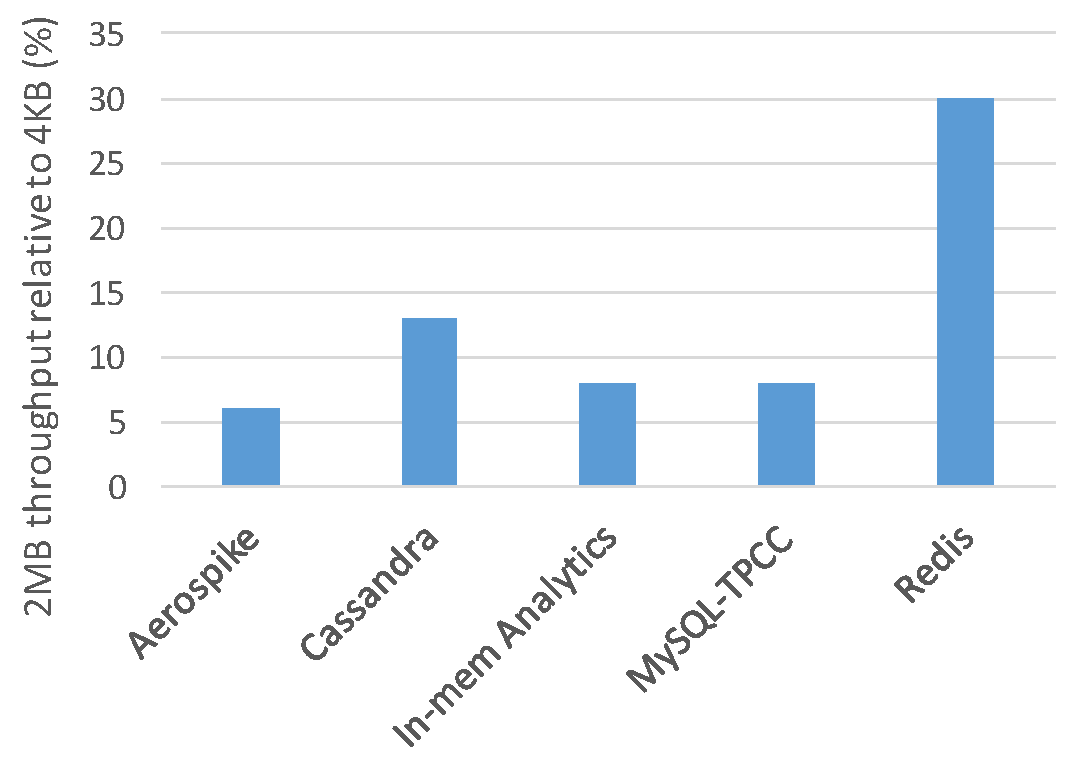
\includegraphics[width=1.0\columnwidth]{figures/thp-perf-improvement.pdf}
%\caption{Throughput improvement by 2MB pages under virtualization relative to
%4KB pages on both host and guest.}
%%\vspace{-0.175in}
%\label{fig:thp-benefit}
%\end{figure}
%

\subsection{Shifting cold data to cheap memory}
\label{analytic-model}

For performance-sensitive and high-footprint cloud applications, it is unlikely that cheaper-but-slower
memory technologies, such as Intel's 3D XPoint memory~\cite{3dcrosspoint}, will 
entirely supplant DRAM main memory.
An increase in memory access latency by even a small multiple (e.g., to 500ns)
will result in drastic throughput losses, as the working set of these applications typically
greatly exceeds cache capacities.
%\fixme{Should we add in a result for slowdown if badger trap traps on every
%page? Neha: not possible, applications stall for very long time durations.}
Because DRAM accounts for only a fraction of total system cost, the net cost of the
throughput loss will greatly outweigh the savings in main memory cost.

However, cloud applications typically have highly skewed access distributions, where
a significant fraction of the application's footprint is infrequently
accessed~\cite{ycsb}.
These rarely accessed pages can be mapped to slow memory without significantly impacting performance.
We refer to this infrequently accessed data as ``cold'' data.

\begin{figure}[t]
\centering
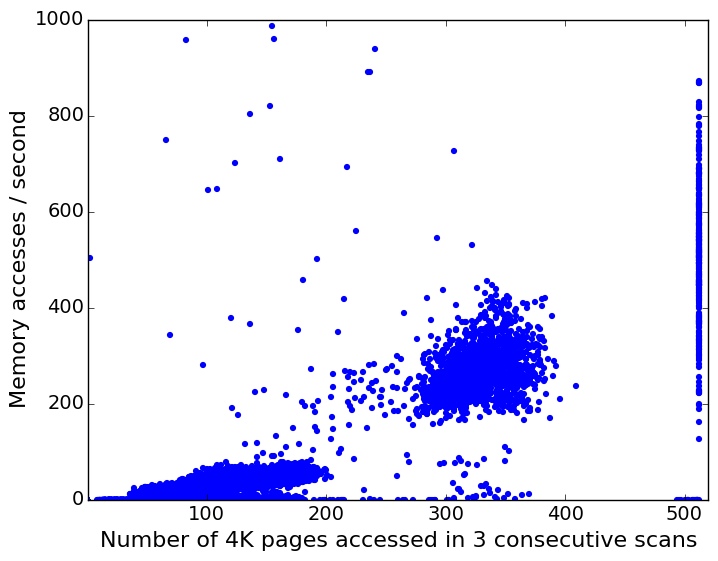
\includegraphics[width=1.0\columnwidth]{asplos2017/figures/redis-plot-3.png}
\caption{Memory access rate vs. hardware {\it Accessed} bit distribution of 4KB
regions within 2MB pages for Redis. The single hardware {\it Accessed} bit per page
does not correlate with memory access rate per page, and thus cannot
estimate page access rates with low overhead.}
\label{fig:redis-access-bit}
\end{figure}

To distinguish cold pages from frequently accessed hot pages, existing
mechanisms exploit the \emph{Accessed} bit in the PTE (set by the hardware each time
the PTE is accessed by a page walk)~\cite{kstaled,vmware-mm,
ref:Guo:2015:PBL:2731186.2731187}. We
investigated one such existing cold-page detection framework, {\tt
kstaled}~\cite{kstaled}. However, we find that the single accessed bit
per page is insufficient to distinguish hot and cold 2MB huge pages with 
sufficiently low overhead. To detect a page access, {\tt kstaled} must clear the
 \emph{Accessed} bit  and flush the corresponding TLB entry.  However, 
 distinguishing hot and cold pages requires monitoring (and hence, clearing)
 accessed bits at high frequency, resulting in unacceptable slowdowns.

Figure~\ref{fig:redis-access-bit} illustrates why hot and cold 2MB huge pages 
cannot be distinguished by temporally sampling
the hardware-maintained access bits at the highest possible rate that can meet
our tight performance degradation target (3\% slowdown), using Redis as an example workload.
The hardware can facilitate 
monitoring at 4KB granularity by temporarily splitting a huge page and monitoring
the accessed bits of the 512 constituent 4KB pages (monitoring at 2MB granularity
without splitting provides even worse hot/cold
differentiation~\cite{ref:Guo:2015:PBL:2731186.2731187}). The horizontal axis 
represents the number of detected ``hot'' 4KB regions
in a given 2MB page when monitoring at the maximum frequency that meets our slowdown target. Here
``hot'' refers to pages that were accessed in three consecutive scan intervals.
The vertical axis represents the ground-truth memory access rate for each 2MB page. 
(We describe our methodology for measuring memory access rate in
Section~\ref{section:access-counting}). 
The key take-away is that the scatter plot is highly dispersed---the spatial frequency
of accesses within a 2MB page is poorly correlated with its true access rate.
Conversely, performance constraints preclude monitoring at higher temporal
frequency. Hence, mechanisms that rely solely on {\it Accessed} bit scanning
cannot identify cold pages with low overhead.

%\begin{table}[t]
%\begin{center}
%\begin{tabular}{|c|c|c|c|}
%\hline
%Scan period&Cassandra& MySQL-TPCC &Redis \\
%\hline
%20 sec& 8\% & 10\% & 15\%\\
%\hline
%\end{tabular}
%\vspace{0.05in}
%\caption{Loose bound on throughput degradation.}
%\label{table:slowmemapprox}
%\end{center}
%\end{table}
%
%To approximate the performance impact of migrating such cold pages to slow memory,
%we develop a loose bound on throughput impact by the following simple analysis. Using the \texttt{kstaled} framework,
%we can measure the number of pages that are not accessed during a given time
%duration. Suppose $P$ pages are not accessed for a time duration $T$. Then,
%we can expect that the access rate to each page in $P$ is $\leq 1/T$ 
%%\fixme{I'm not sure this math follows. We need to talk about this more.}. 
%Now,
%assuming that we place the $P$ pages in slow memory, and that each slow
%memory reference has a latency of $t_{slow}$, we can see that the {\it extra}
%time required for accessing slow memory $\leq t_{slow}P/T$. Thus, the benchmark
%throughput will be degraded by $\leq t_{slow}P/T$. In
%Table~\ref{table:slowmemapprox} we show the value of this rough bound on
%throughput degradation.
%
%From Table~\ref{table:slowmemapprox} we can see that for $T = 20s$, i.e.,
%placing all pages that are cold for 20s into slow memory, the performance
%degradation is $\leq 15\%$. Note that our model is conservative, since it
%doesn't consider that many of the detected ``cold'' pages are, in fact, idle for
%even longer periods and have much lower access frequencies than
%$1/T$.
%Nevertheless, this analysis suggests that a large fraction of
%the application footprint can be migrated to slow memory in cloud workloads. In fact, as we
%show in the remainder of this paper, the actual performance impact on the
%application performance is much lower than the simple analytical model predicts
%($\leq 5\%$ for MySQL and Cassandra, and $\leq 10\%$ for Redis).
%
\subsection{Benefits of transparent huge pages}
Intel's IA-64 x86 architecture mandates a 4-level page table structure for 4KB
memory pages.  So, a TLB miss may incur up to four memory accesses to walk the page table. 
Under virtualization, with two-dimensional page table walks (implemented in Intel's
Extended Page Tables and AMD's Nested Page Tables), the cost of a page walk can be as high as
24 memory accesses~\cite{Intel-sw-manual, AMD-NPT}.  When memory is mapped to a 2MB 
huge page in both the guest and host, the worst-case page walk is reduced to 15 accesses, which 
significantly lowers the performance overhead of virtualization. Moreover,
2MB huge pages increase the TLB reach and improve the cacheability of intermediate
levels of the page tables, as fewer total entries compete for cache capacity. 

Table~\ref{tab:thp-benefit} shows the performance benefit of using huge pages
via Linux's Transparent Huge Page (THP) mechanism. We compare throughput of
various cloud applications where both the guest and host employ 2MB huge pages
against configurations with transparent huge pages disabled (i.e., all pages are
4KB). We observe significant throughput benefits as high as 30\% for Redis.
Previous literature has also reported performance benefits of huge
pages~\cite{ref:Guo:2015:PBL:2731186.2731187, Basu2013, hugepages}. From these
results, it is clear that huge pages are essential to performance, and any
attempt to employ a dual-technology main memory must preserve the performance
advantages of huge pages. For this reason, we only evaluate Thermostat with THP
enabled at both host and guest.

%\subsection{Identifying cold data is hard}
%Identifying cold data in applications has been a challenging problem, more so in
%the case where cold data becomes hot later on the application run time. Linux
%kernel developers have built cold data detection mechanisms at run time for any
%given page size granularity ~\cite{kstaled, vmware-mm}. However, those
%mechanisms cannot be used to detect what we call hotspot 4KB pages in otherwise
%cold pages in the applications at run time. Figure~\ref{fig:motivation} shows
%percentage of application data that remains untouched for 20 sec time duration
%at 4KB and 2MB granularity~\footnote{Note that in ARM based architectures huge
%size can be as low as 64KB. However, due to prevalence of x86 based server chips
%we experimented with x86 based machines only.}. Fraction of cold data decreases
%from 50\% to only 20\% as page size granularity is increased from 4KB to 2MB.
%For employing cheaper but slower memory we want large fraction of application
%data to be cold so as to minimize the rate of slow memory access. When using 2MB
%pages there is an opportunity to detect larger fraction of cold data in
%applications that current mechanisms fail to identify. 

%\subsection{Previous techniques are inadequate}
%Why are previous 2-level memory techniques inadequate in solving this issue.
%
%Re-iterate the problem we are solving and the central idea of our solution.

\section{Thermostat}
\label{proposal}

We present Thermostat, an application-transparent huge-page-aware mechanism to
detect cold pages during execution. The input to Thermostat is a user-specified
tolerable slowdown (3\% in our evaluation) incurred as a result of Thermostat's 
monitoring and due to accesses to data shifted to slow memory. Thermostat periodically
samples a fraction of the application footprint and uses a page poisoning technique
to estimate the access rate to each page with tightly controlled overhead. The
estimated page access rate is then used to select a set of pages to
place in cold memory, such that their aggregate access rate will not result in 
slowdown exceeding the target
performance degradation.  These cold pages are then continually monitored to
detect and rapidly correct any mis-classifications or behavior changes.
In the following sections, we describe the Thermostat in more detail.

\begin{figure*}[t]
\centering
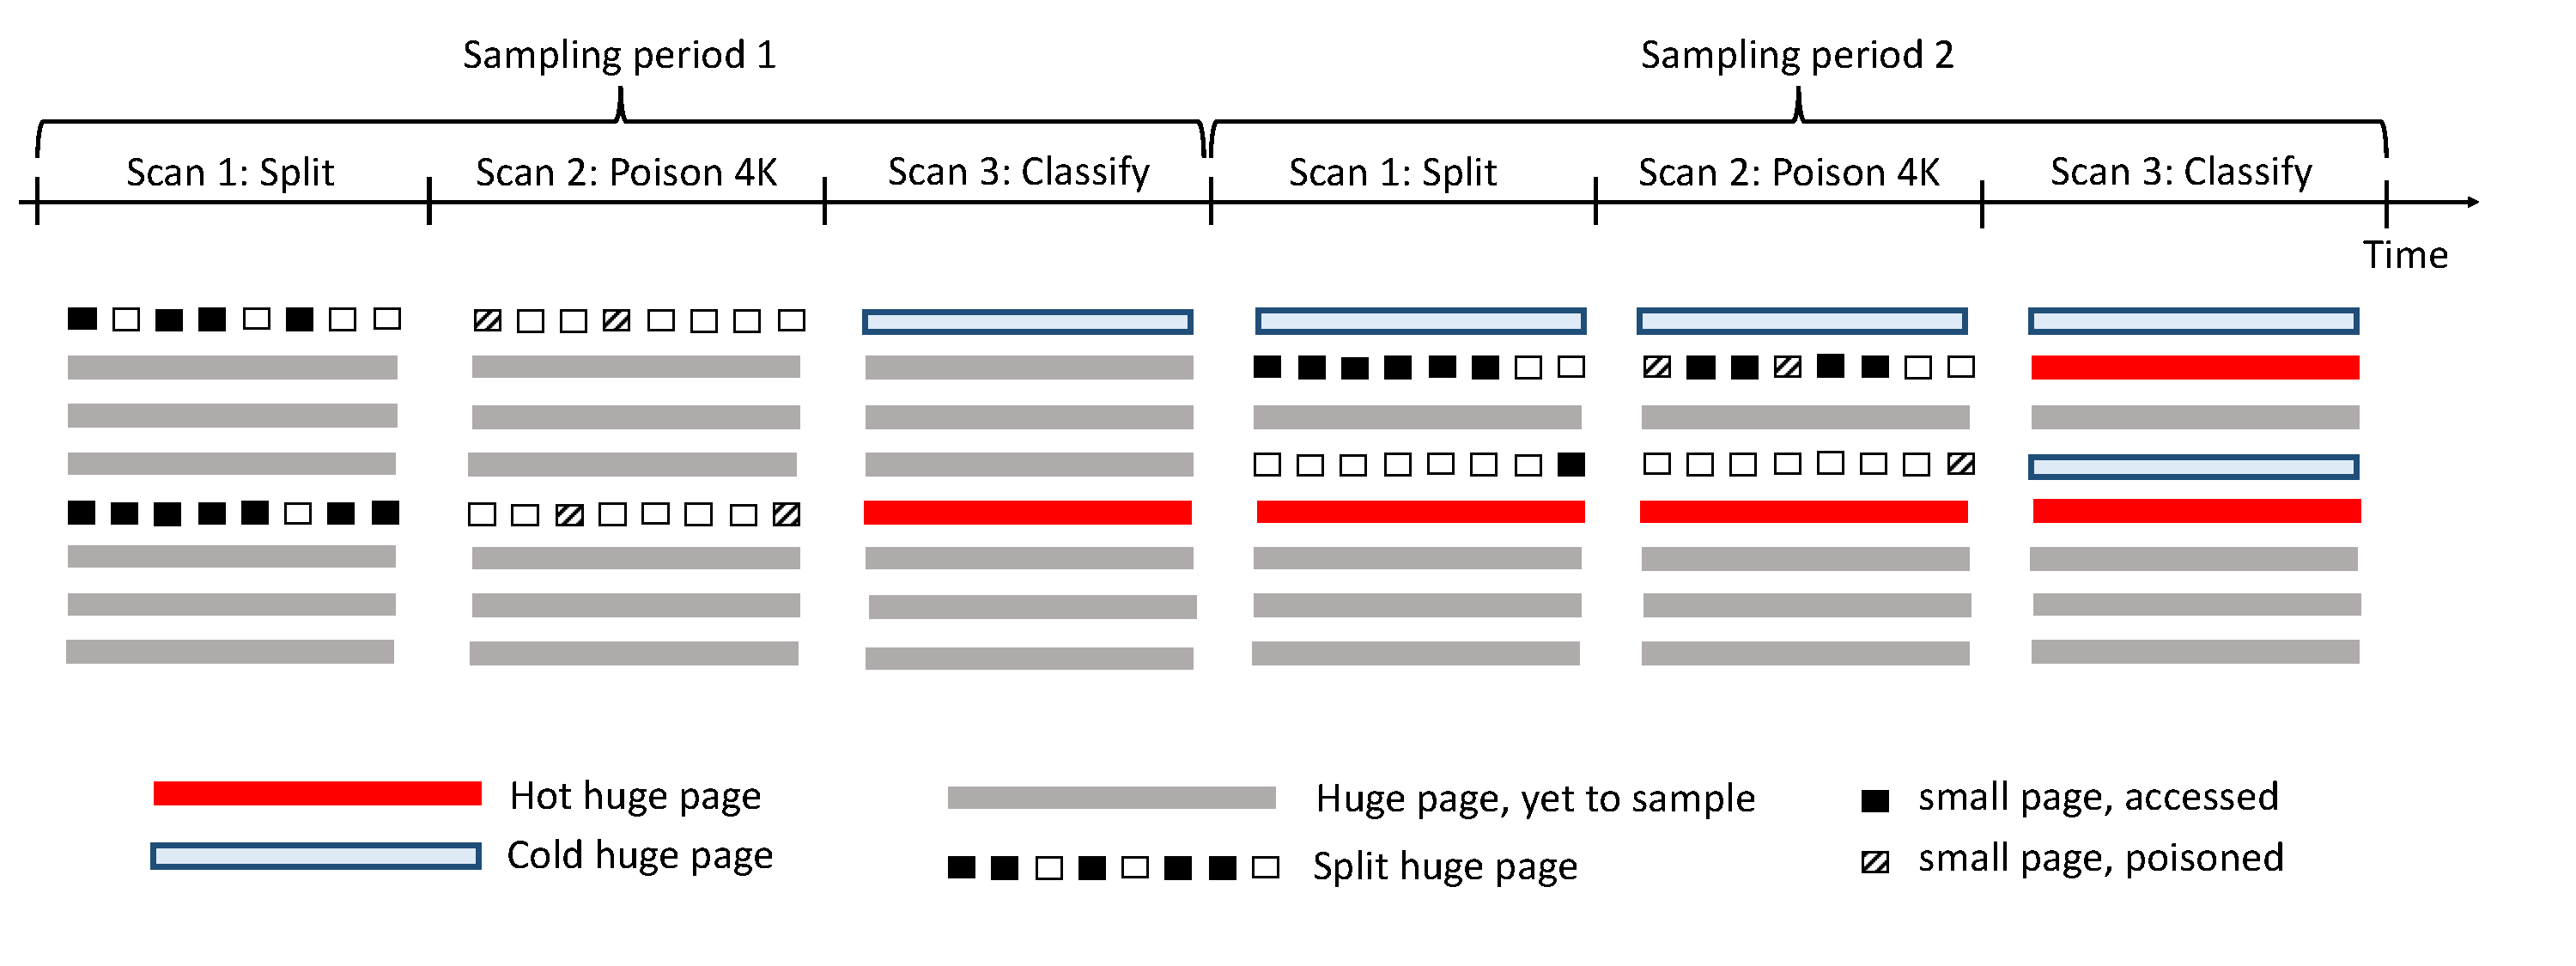
\includegraphics[width=1.0\textwidth]{asplos2017/figures/new-policy-sampling-figure.pdf}
\caption{Thermostat operation: Thermostat classifies huge pages into hot and cold by randomly splitting a
fraction of pages and estimating huge page access rate by poisoning a fraction of 4K
pages within a huge page. The sampling policy is described in
Section~\ref{page-sampling}, Section~\ref{section:access-counting} describes our
approach to page access counting, and Section~\ref{page-classification} describes
the page classification policy. Note that the sampling and poisoning fractions here
are for illustration purposes only. In our evaluation we sample 5\% of huge pages
and poison at most 50 4KB pages from a sampled huge page.}
\label{fig:sampling}
\end{figure*}

\subsection{Overview}
We implement Thermostat in the Linux 4.5 kernel. Thermostat can be controlled at
runtime via the Linux memory control group (cgroup) mechanism~\cite{cgroups}.
All processes in the same cgroup share Thermostat parameters, such as the
sampling period and maximum tolerable slowdown.

The Thermostat mechanism consists of four components: (i) a sampling mechanism
that randomly selects a subset of pages for access rate monitoring, (ii) a monitoring
mechanism that counts accesses to sampled pages while limiting maximum overhead, 
(iii) a classification policy to select pages to place in slow memory, and,
(iv) a mechanism to monitor and detect mis-classified pages or behavior changes and migrate 
pages back to conventional (fast) memory.

The key challenge that Thermostat must address is the difficulty of discerning the access 
rates of 2MB pages at a sufficiently low overhead while still responding rapidly
to changing workload behaviors. Tracking the access rate of a page
is a potentially expensive operation if the page is accessed frequently.  
Hence, to bound the performance impact of
access rate monitoring, only a small fraction of the application footprint may be
monitored at any time.  However, sampling only a small fraction of the application
footprint leads to a policy that adapts only slowly to changes in memory behavior.

\subsection{Page sampling}
\label{page-sampling}
Sampling a large number of huge pages is desirable as it leads to quick
response to time-varying workload access patterns. But, it can lead to a
high performance overhead, since, as explained in
Section~\ref{section:access-counting}, each TLB miss to a sampled page incurs additional
latency for OS fault handling. To tightly control application performance
slowdown, {\it we split a random sample of huge pages (5\% in our case)
into 4KB pages, and poison only a fraction of these 4KB pages in each sampling interval}.
Below, we detail the strategy used to select which 4KB pages to poison, and how
we estimate the total access rate from the access rates of the sampled 4KB
pages.

A simple strategy to select 4KB pages from a set of huge pages is to select $K$
random 4KB pages, for some fixed $K$ ($K = 50$ in our evaluation). However, when only a few 4KB
pages in a huge page are hot, this naive strategy may fail to sample them, and
thus deem the overall huge page to have a low access rate. To address this shortcoming, 
our mechanism monitors page access rates in two steps.
We first rely on the hardware-maintained {\it Accessed} bits to monitor all 512 4KB pages
and identify those with a  non-zero access rate.  We then monitor a sample of these 
pages using our more costly
software mechanism to accurately estimate the aggregate access rate of 
the 2MB page. With our strategy, {\it only 0.5\% of overall 4KB pages are
sampled at any time} -- which makes the performance overhead due to sampling
$<$ 1\%.

To compute the aggregate access rate at 2MB granularity from the access rates of the sampled
4KB pages, we scale the observed access rate in the sample by the total number
of 4KB pages that were marked as accessed. The monitored 4KB pages comprise a 
random sample of accessed pages, while the remaining pages have a negligible
access rate.

\subsection{Page access counting}
\label{section:access-counting}
Current x86 hardware does not support access counting at a per-page granularity.
Thus, we design a software-only solution to track page access rates with very
low overhead ($<$1\%) by utilizing PTE reserved bits. In
Section~\ref{counting_hardware}, we discuss two extensions to existing x86
mechanisms that might enable lower overhead page access counting.

To approximate the number of accesses to a page, we use BadgerTrap, a kernel
extension for intercepting TLB misses~\cite{ref:badgertrap}. When a page is
sampled for access counting, Thermostat poisons its PTE by setting a reserved
bit (bit 51), and then flushes the PTE from the TLB.  The next access to the
page will incur a hardware page walk (due to the TLB miss) and then trigger a
protection fault (due to the poisoned PTE), which is intercepted by BadgerTrap.
BadgerTrap's fault handler unpoisons the page, installs a valid translation in
the TLB, and then repoisons the PTE. By counting the number of BadgerTrap
faults, we can estimate the number of TLB misses to the
page, which we use as a proxy for the number of memory accesses.

Note that our approach assumes that the number of TLB misses and 
cache misses to a 4KB page are similar.  For hot pages, this assertion does not
hold.  However, Thermostat has no need to accurately estimate the access rate
to hot pages; it is sufficient to know that they are hot.  Conversely, for cold pages
nearly all accesses incur both TLB and cache misses as there is no temporal
locality for such accesses, and, therefore, tracking
TLB misses is sufficient to estimate the page access rate. We validated our 
approach by measuring
the TLB miss rates (resulting in page-walks) and last-level cache miss rates for
our benchmark suite using hardware performance counters via the Linux {\tt perf}
utility. For pages we identify as cold, the TLB miss rate is typically higher (but
always within a factor of two) of the last-level cache miss rate measured
without BadgerTrap, indicating that our approach is reasonable.

\subsection{Page classification}
\label{page-classification}
Classifying pages as hot or cold is governed by the user-specified maximum
tolerable slowdown (without such a threshold, one can simply declare all
pages cold and call it a day). To select cold pages, we use the estimated access
rates of each (huge) page.

We translate a tolerable slowdown of $x\%$ to an access rate
threshold in the following way. Given $A$ accesses to slow memory in one second,
the total time consumed by slow memory accesses is $At_s$, where $t_s$ is the
access latency of the slow memory.
Thus, a slowdown threshold of $x\%$ can be translated to an access rate
threshold of $\frac{x}{100t_s}$ per second. If a fraction $f$ of the total
huge pages were sampled, we assign pages to the slow memory such that their
aggregate estimated access rate does not exceed
$f\frac{x}{100t_s}$. We sort the sampled huge pages in increasing
order of their estimated access rates, and then place the coldest pages in slow
memory until the total access rate reaches the target threshold.

This simple approach governs the access rate to slow memory to avoid the
user-specified degradation target. In Figure~\ref{fig:fault-rate}, we
show slow memory access rate averaged over 30 seconds for our benchmark suite,
assuming 1us slow memory access latency and 3\% tolerable slowdown (we discuss
detailed methodology in Section~\ref{section:methodology}). We observe that
Thermostat keeps the slow memory access rate close to the target 30K
accesses/sec. For Aerospike and Cassandra slow memory access rate
temporarily exceeds 30K accesses/sec but is brought back below 30K accesses/sec by 
mis-classification detection, discussed next in
Section~\ref{classification-correction}.

\subsection{Correction of mis-classified pages}
\label{classification-correction}
Since we estimate the access rate of a huge page based on the access rates
of only a few (not more than 50, as described in
Section~\ref{page-sampling}) 4KB pages, there is always some probability
that some hot huge pages will be mis-classified as cold due to sampling error. 
Such mis-classifications are detrimental to application
performance, since the interval between successive samplings of any given
huge page can be fairly long. To address this issue, we track the number of
accesses being made to each cold huge page, using the software
mechanism mentioned in Section~\ref{section:access-counting}.  Since the access
rate to these pages is slow by design, the performance impact of this monitoring is low.
In every sampling period we sort the huge pages in slow memory by their access
counts. All the huge pages in slow memory are migrated back to fast memory which
exceed the cumulative tolerable access rate to slow memory. In addition to the
mis-classified pages we also identify pages that become hot over time, adapting
to the change in application's hot working set.
%A huge page in slow memory is migrated back to fast memory if its actual access rate 
%exceeds its previously estimated access rate. 
%In addition, we do not migrate back a page if its actual rate is less than 50
%accesses/second to prevent thrashing behavior for cold pages with
%unstable access rates.

\begin{figure}[t]
\centering
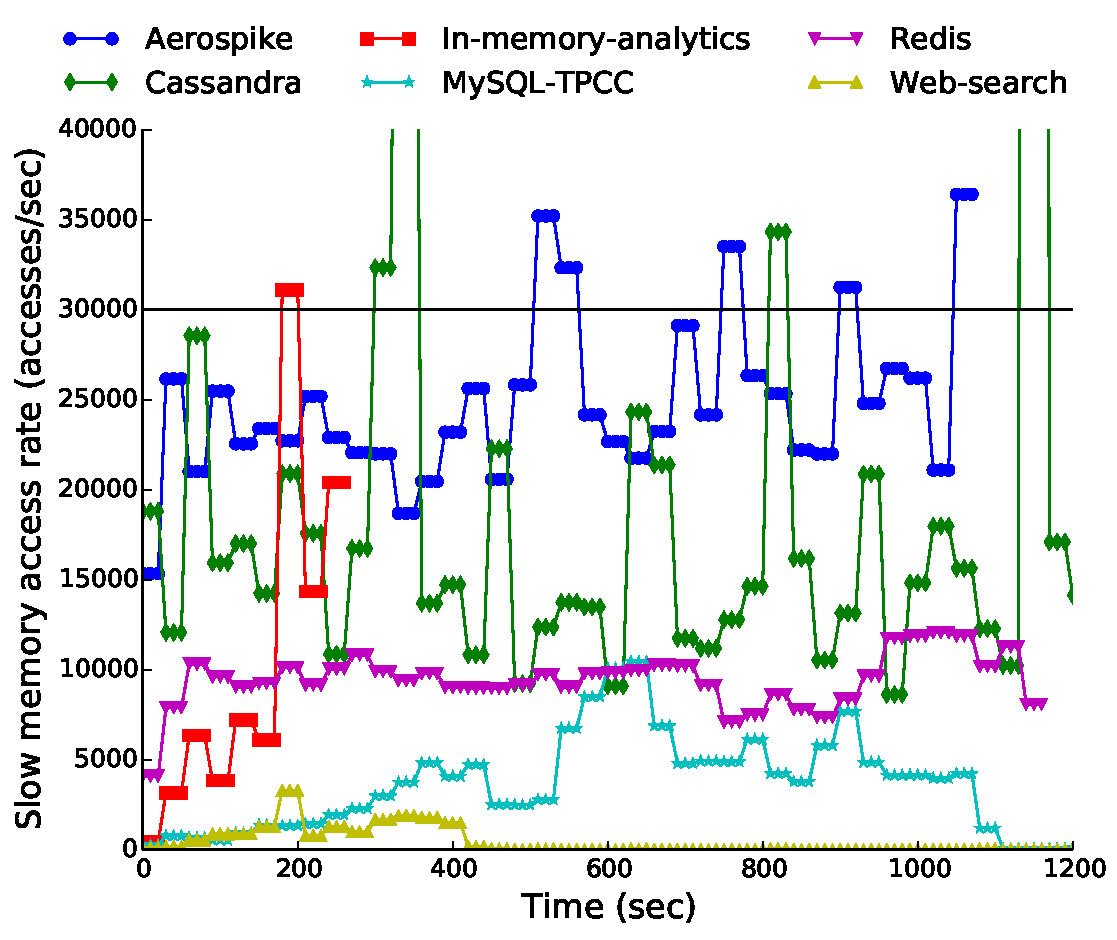
\includegraphics[width=1.0\columnwidth]{asplos2017/figures/faults.pdf}
\caption{Slow memory access rate over time. For a 3\% tolerable slowdown and 1us
slow memory access latency, the target slow memory access rate is 30K accesses/sec.
Thermostat tracks this 30K accesses/sec target. Note that different benchmarks
have different run times; we plot x-axis for 1200 seconds.} 
\label{fig:fault-rate}
\end{figure}

\subsection{Migration of cold pages to slow memory}
Once cold pages have been identified by the guest, they must be migrated to 
the slow memory. We use the NUMA support in KVM guests to achieve this transfer. The NVM
memory space is exposed to the guest OS as a separate NUMA zone, to which the guest
OS can then transfer memory. NUMA support in KVM guests already exists in Linux
and can be used via {\tt libvirt}~\cite{libvirt-numa}.

\subsection{Thermostat example}
Figure~\ref{fig:sampling} illustrates Thermostat's page classification for an
example application with eight huge pages. Each sampling period comprises 
three stages: (i) split a fraction of huge pages, (ii) poison a fraction of split and
accessed 4KB pages, record the access count to 4KB pages to estimate access rate
of the huge pages, and, (iii) classify pages as hot/cold. In this example, we sample 25\% of
huge pages (two huge pages out of eight are sampled). In the first sampling
period, Thermostat splits and records 4KB-grain accesses to two pages (page 1
and 5) in the first scan period. In the second scan period 4KB pages 1 and 4
of the first huge page and 3 and 8 of the fifth huge page are selected to be poisoned.
Thermostat then estimates the access rate to huge page 1 and 5 by from the access rates
of the 4KB pages.  Finally, Thermostat sorts the estimated access rates of the huge pages
and classifies page 1 as cold, as its estimated access rate is below
the threshold tolerable slow memory access rate. However, because the sum of the
access rates of both huge pages is above the threshold access rate, page 5 is classified
as hot. Similarly, in the second sampling period, pages 2 and 4 are randomly
selected for sampling. At the end of the sampling period page 2 is classified as
hot and page 4 as cold.

%\subsection{Linux implementation}
%We implement Thermostat in Linux kernel version 4.5. We add a vector data
%structure using {\tt kmalloc} to track sampled pages storing {\tt struct page}
%pointers and there access rates while sampling.  \fixme{Note that this data
%structure only stores two int type data, hence a low overhead space cost giving
%high returns in overall memory savings.} We split huge pages and merge them in
%place. We piggy back on Linux's {\tt split\_huge\_pmd} functionality to split
%pages and merge small pages back by a custom function similar to {\tt
%khugepaged}'s {\tt collapse\_huge\_page}. We patched in {\tt kstaled} to monitor
%access bit in PTEs~\cite{kstaled}. We use BadgerTrap to poison pages to monitoe
%access rates~\cite{ref:badgertrap}.
%\subsubsection{Thermostat on host system}
%The publicly available version of {\tt kstaled} examines PTEs and PMDs for detecting
%accesses to pages. However, due to reasons discussed in Section~\ref{discussion}, running
%Thermostat on the host is preferable as opposed to in the guest. To use
%Thermostat on
%the host, we modified {\tt kstaled} to examine the accessed bit information in Shadow
%PTEs (SPTE), which is the host page table part of a two-dimensional page table.
%In x86-64, the accessed bits of both PTEs (in guest) and SPTEs (in host) are set
%when a page walk occurs. In case of multiple guests sharing the same physical
%page, the {\tt mmu\_notifier} interface of KVM allows us to go through all the
%VMs in which the page is mapped, and get the accessed information of that page
%by OR-ing the Accessed bits from all the SPTEs.
%
%
%
%Using the Accessed bit, Thermostat can measure whether a page
%was accessed in a given ``scan period'' or not. However, it is difficult to
%judge the hotness of a page based only on a single accessed/not accessed
%outcome. \todo{Also, as we show in Section XXX, a single Accessed bit
%observation can be noisy, and can lead to unnecessary migrations between NVM and
%DRAM.} To solve these problems, we sample the pages for more than one scan
%period. The time period for which pages are sampled is denoted by ``sampling
%period'' (set to 2 scan periods in our experiments). Sampling for multiple scan
%periods allows us to do robust cold page detection, as shown in Section XXX.
%After the sampling period is over, the hugepages are categorized as hot or cold
%by the Thermostat policy outlined next.
%
%
%
%
%\textbf{Page Cache:}Interaction of Kstaled mechanism with unmapped pages,
%e.g., page cache: \todo{Say something here.}
%
%
%\subsection{Translation Facades}
%Second, the Thermostat controller needs an effective mechanism for chunking up a DRAM
%huge page into several small pages, and also for compacting several small hot
%pages into a single DRAM huge page. Chunking up a huge page is relatively simple
%-- one need only allocate several page table entries (PTEs) corresponding to the
%chunked up page. Doing the inverse, that is compacting several small pages from
%the slow-mem and DRAM into a single DRAM huge page has more challenges. First,
%due to memory fragmentation, it may not be possible to find a suitable space to
%put the newly created huge page. Second, reading several small pages from
%slow-mem, and creating a huge page out of them can be a potentially very long
%latency operation, which can then affect application throughput as well as tail
%latency. We plan to study the design trade-off space of when to perform
%these operations and incorporate the obtained insights into building the Thermostat
%controller.

\section{Methodology}
\label{section:methodology}

\subsection{System Configuration}
We study Thermostat on  a 36-core (72 hardware thread) dual-socket
x86 server, Intel Xeon E5-2699 v3, with 512 GB RAM running Linux 4.5.
Each socket has 45MB LLC. There is a 64-entry TLB per core and a shared 1024
entry L2 TLB. Several of our benchmark applications perform frequent I/O and are
highly sensitive to OS page cache performance.
To improve the page cache, we install {\tt hugetmpfs}, a mechanism that
enables use of huge pages for the {\tt tmpfs}~\cite{hughd-hugetmpfs} filesystem. 
We place all files accessed by the benchmarks in {\tt tmpfs}. In the future, we expect
that Linux may natively support huge pages in the page cache for other file
systems.

We run the benchmarks inside virtual machines using the Kernel-based Virtual
Machine (KVM) virtualization platform.  Client threads, which generate traffic to the
servers, are run outside the virtual machine, on the host OS. We run the client threads 
and server VM on the same system and use a bridge network with virtio between host 
and guest so that network performance is not a bottleneck.
We isolate the CPU and
memory of the guest VM and client threads on separate sockets using 
Linux's control group mechanism~\cite{cgroups} to avoid performance interference.  
The benchmark VM is allocated 8 CPU cores, a typical medium-sized cloud 
instance.
We set the Linux frequency governor to ``performance'' to
disable dynamic CPU frequency changes during application runs. 

\subsection{Emulating slow memory: BadgerTrap}
\label{slow-memory}
Dual-technology main memory, in particular Intel/Micron's 3D XPoint memory, 
is not yet available.  
Hence, we use a software technique to emulate slow memory while placing all
data in conventional DRAM.

Each cache miss to slow memory should incur an access latency that is a multiple 
of the DRAM latency (e.g., 400ns slow memory~\cite{ref:Dulloor:datatiering} vs. 
50ns DRAM latency).
There is no easy mechanism to trap to software on all cache misses. Instead,
we introduce extra latency by inducing page faults upon translation misses (TLB misses) 
to cold pages by using BadgerTrap~\cite{ref:badgertrap}. 
%This mechanism is similar to 
%how Thermostat measures page access frequency.

The software fault mechanism is an approximation of an actual slow memory device.
The BadgerTrap fault latency (about 1us in our kernel) is higher than some authors
predict the 3D XPoint memory read latency will be~\cite{ref:Dulloor:datatiering}.  Furthermore, the poisoned PTE
will induce a fault even if the accessed memory location is present in the hardware 
caches. In these two respects, our approach over-estimates the penalty of slow 
memory accesses.  However, once BadgerTrap installs a (temporary) translation, 
further accesses to other cache blocks on the same slow-memory page will not 
induce additional faults, potentially under-estimating impact. Our testing with micro benchmarks
indicates our approach yields an average access latency to slow memory in the 
desired range, in part, because slow-page accesses are sufficiently infrequent that
they nearly always result in both cache and TLB misses anyway, as we discuss in
Section~\ref{section:access-counting}.
%On balance, we expect the differences between
%TLB and cache misses to have little impact because, by design, Thermostat places
%only rarely accessed pages in cold memory.

%We validate that BadgerTrap provides a reasonable approximation of slow memory
%by measuring the TLB and cache miss rates for our benchmark suite using hardware
%performance counters.  The TLB miss rate induced by BadgerTrap is typically higher 
%(but always within a factor of two) than the last-level cache miss rate measured 
%without BadgerTrap, indicating that our performance estimates are conservative.
%\fixme{Neha: Verify this number for all the new benchmarks.}

One important detail of our test setup is that we must install BadgerTrap (for the purpose 
of emulating slow memory latency) within
the guest VM rather than the host OS.  Thermostat communicates with the guest-OS 
BadgerTrap instance to emulate migration to slow memory.  We must install
BadgerTrap within the guest because, otherwise, each BadgerTrap fault would 
result in a {\tt vmexit}.  In addition to drastically higher fault latency, {\tt vmexit} operations
have the side-effect of changing the Virtual Processor ID (VPID) to 0. Since KVM
uses VPIDs to tag TLB entries of its guests, installing a TLB entry with the
correct VPID would entail complexity and incur even higher emulation latency.
% than
%involve a significantly complex operation of re-entering the
%VM, performing a single memory operation and jumping back, which would incur
%even more emulation latency.
Since BadgerTrap on the guest entails a latency of
$\approx$ 1$\mu$s, which is already higher than projected slow-memory latencies~\cite{ref:Dulloor:datatiering},
we did not want to incur additional slowdown by emulating slow memory in the
host OS.


%To ensure that this approach is
%reasonable, we obtained the TLB and cache miss rates for the applications under
%study by {\tt perf}. We observed that in Cassandra and MySQL-TPCC the TLB miss
%rate (resulting into page walks)
%was 2$\times$ higher than the last level cache miss rate, meaning that we will only be
%overestimating the performance impact. In Redis, however, the TLB miss rate is
%2$\times$ lower than the cache miss rate. 

%{\textbf{Why not Badgertrap on the host?}


\subsection{Benchmarks}
\label{benchmarks}
We evaluate Thermostat with applications from Google's Perfkit Benchmarker and
the Cloudsuite benchmarks~\cite{perfkitbenchmarker, cloudsuite}. These
applications are representative server workloads that have large memory
footprints and are commonly run in virtualized cloud environments.  We do not
evaluate Thermostat for general-purpose GPU applications since non-volatile memory
technologies are expected to have much lower bandwidth than high-bandwidth
graphics memories -- even lower than DDR memory technologies -- thus are not a
suitable match to memory bandwidth-sensitive platforms like GPUs.

{\bf TPCC on MySQL:} TPCC is a widely-used database benchmark, which aims to measure
the transaction processing throughput of a relational database~\cite{tpcc}. We 
execute TPCC on top of MySQL, one of the most popular open-source database 
engines, which is often deployed in the cloud.  We use the open-source
TPCC implementation from OLTP-Bench~\cite{oltpbench} (available at
\url{https://github.com/oltpbenchmark/oltpbench}). We use a scale factor of
320, and run the benchmark for 600 seconds after warming up for 600 seconds.
MySQL makes frequent I/O requests and hence benefits markedly from our use
of {\tt hugetmpfs} to enable huge pages for the OS page cache.
%We observe 380
%transactions/sec throughput for our baseline system with all pages in DRAM as
%huge pages.

{\bf NoSQL databases:} Aerospike, Cassandra, and Redis are popular NoSQL
databases~\cite{aerospike, cassandra, redis}.
Cassandra is a wide-column database designed to offer a variable number of fields
(or columns) per key, while Redis and Aerospike are simpler key-value databases 
that have higher peak throughput. Redis is single-threaded whereas Aerospike is
multi-threaded.
Cassandra performs frequent file I/O as it periodically compacts its SSTable
data structure on disk~\cite{ref:sstable}. So, Cassandra also benefits substantially
from {\tt hugetmpfs}. Redis performs no file I/O after loading its dataset into memory.

We tune Aerospike, Cassandra, and Redis based on the settings provided by
Google's Perfkit Benchkmarker for measuring cloud
offerings~\cite{perfkitbenchmarker}.  We use the YCSB traffic generator to drive
the NoSQL databases~\cite{ycsb}. For Aerospike we use 200M operations
and for Cassandra we use 50M operations on 5M keys with 20 fields each with a
Zipfian distribution.
For both of these application, we evaluate two workload mixes: a read-heavy load
with 95:5 read/write ratio and a write-heavy load with 5:95 read/write ratio. For Redis, we
access keys with a hotspot distribution, wherein 0.01\% of the keys account for
90\% of the traffic. We vary value sizes according to the
distribution reported in~\cite{facebook-key-value}. We observe 176K
and 215K operations/sec for read-heavy and write-heavy workloads for Aerospike,
and 21K and 45K operations/sec for read-heavy and write-heavy workloads for
Cassandra. For Redis we observe 188K
operations/sec for our baseline system with all pages in
DRAM as huge pages.

{\bf In-memory analytics:} We evaluate Thermostat on in-memory analytics
benchmarks from Cloudsuite~\cite{cloudsuite}. In-memory analytics runs a
collaborative filtering algorithm on a dataset of user-movie ratings.  It uses
the Apache Spark framework to perform data analytics. We set both executor and driver
memory to be 6GB to execute the benchmark entirely in memory. We run the benchmark to
completion, which takes 317 seconds for our baseline system with all pages in
DRAM as huge pages.

{\bf Web search:} Cloudsuite's web search uses the Apache Solr search engine
framework. We run client threads on host and index nodes within the virtual
machine. We set steady state time to be 300 seconds and keep default values for all
the other parameters on the client machine. As specified by the benchmark,
target response time requires 99\% of the requests to be serviced in 200ms. For
our baseline system with all pages in DRAM as huge pages, we observe 50
operations/sec with $\approx$ 85ms 99th percentile latency.
%{\bf Tomcat:} Tomcat is a popular web server frontend. We use the {\tt wrk}
%(available at \url{https://github.com/wg/wrk}) tool to generate XXX requests to
%the webpage \texttt{XXX.XXX} using XXX parallel clients. Our installation runs
%at the peak throughput at this load. 

\subsection{Runtime overhead of Thermostat Sampling}
We measure the runtime overhead of Thermostat to ensure that application 
throughput is not degraded by Thermostat's page sampling mechanism.
For sampling periods of 10s or higher, we observe negligible CPU activity
from Thermostat and no measurable application slowdown ($<$ 1\%).


\begin{table}[t]
\begin{center}
\begin{tabular}{|l|l|l|}
\hline
& Resident Set Size& File-mapped\\
\hline
Aerospike & 12.3GB & 5MB\\
\hline
Cassandra & 8GB & 4GB\\
\hline
MySQL-TPCC & 6GB & 3.5GB\\
\hline
Redis & 17.2GB & 1MB\\
\hline
%Graph-analytics & 16.6GB & 1MB\\
%\hline
In-memory-analytics & 6.2GB & 1MB\\
\hline
Web-search & 2.28GB & 86MB\\
\hline
\end{tabular}
%\vspace{0.05in}
\caption{Application memory footprints: resident set size and file-mapped pages.}
\label{tab:memory-footprint}
\end{center}
\end{table}

\section{Evaluation}
\label{results}

We next measure Thermostat's automatic hot/cold classification and run-time
placement/migration mechanisms on our suite of cloud applications.

Thermostat takes as input a tolerable slowdown; a single input parameter 
specified by a system administrator.  It then automatically selects cold pages
 to be migrated to slow memory at runtime. We set a tolerable slowdown of
3\% throughout our evaluation, since a higher slowdown may lead to an overall
cost increase due to higher required CPU provisioning (which is more expensive
than memory). Thermostat's slowdown threshold can be 
changed at runtime through the Linux cgroup mechanism. Hence,
application administrators can
dynamically tune the threshold based on service level agreements
for latency-critical applications or for the throughput requirements of
batch jobs.  We show that, for our application suite, Thermostat meets the
target 3\% slowdown while placing a significant fraction of application footprint in slow memory
dynamically at runtime.

%Based on the characterization results shown in Figure~\ref{fig:cassandra-hotspot},
%we set an objective of migrating roughly half of the application memory footprint
%to slow memory with an expected performance degradation of 5\% for Cassandra
%and TPCC.  However, for Redis, the memory access locality pattern is flat, and
%a 5\% degradation target allows only a small fraction of the footprint to be classified
%as cold.  Hence, for Redis, we set a 10\% degradation target.

We evaluate Thermostat with 5\% of huge pages sampled in every scan interval of
30s and at most 50 4KB pages poisoned for a sampled huge page.
We compare the performance of Thermostat with a placement policy that
places all pages in DRAM, which maximizes performance while incurring maximal 
memory cost.  Thermostat's sampling mechanisms incur a negligible performance
impact (well under 1\%)---the slowdowns we report are entirely attributable to 
slow memory accesses. 

We briefly discuss our findings for each application. Table~\ref{tab:memory-footprint} reports each 
application's footprint in terms of resident set size (RSS) and file-mapped
pages. The memory savings quoted for each benchmark is the average cold memory
fraction over the benchmark's runtime.

\begin{figure}[t]
\centering
%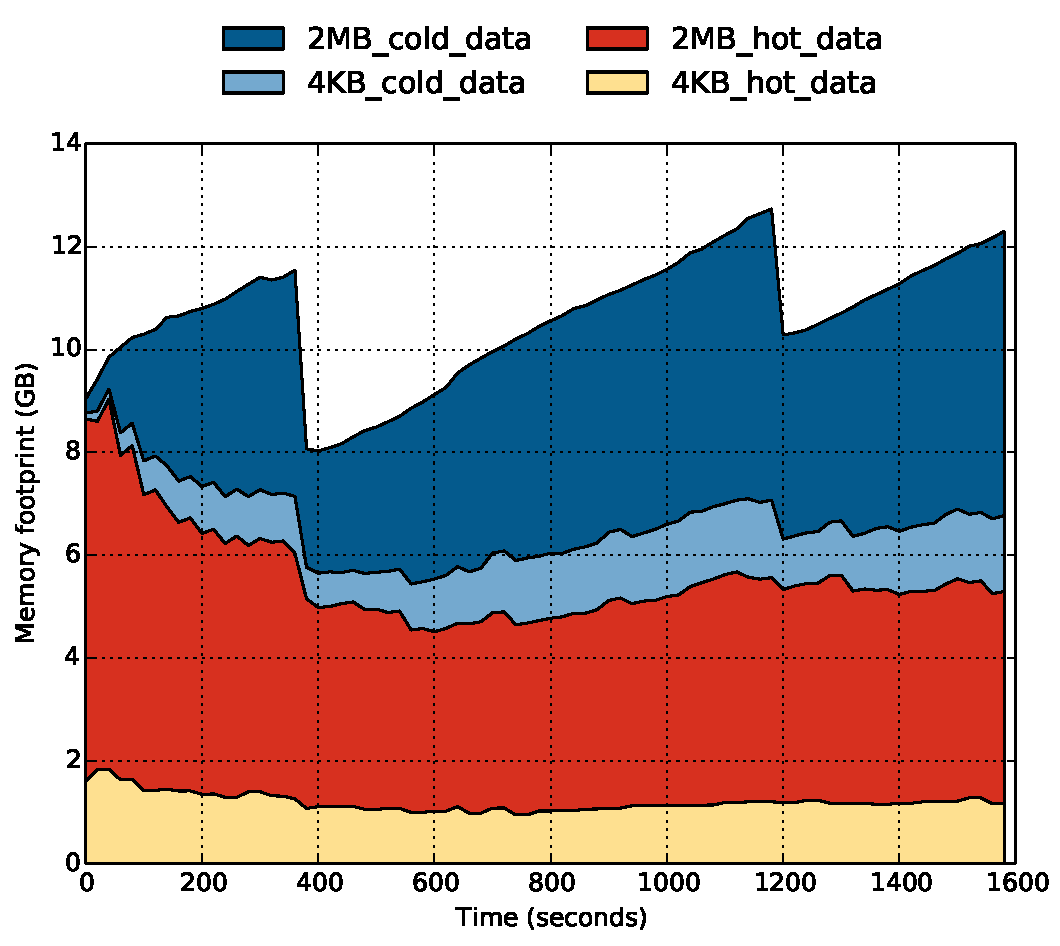
\includegraphics[width=1.0\columnwidth]{figures/cassandra-capacity.pdf}
\includegraphics[width=0.8\columnwidth]{asplos2017/figures/cassandra-new-set-policy-kstaled10-sample5-period3-capacity_over_time.pdf}
\caption{Amount of cold data in Cassandra identified at run time with 2\%
throughput degradation for a write-heavy workload (5:95 read/write ratio).}
\label{fig:cassandra-capacity}
\end{figure}

\begin{figure}[t]
\centering
%\includegraphics[width=1.0\columnwidth]{figures/tpcc-capacity.pdf}
\includegraphics[width=0.8\columnwidth]{asplos2017/figures/tpcc-clipped-new-policy-capacity_over_time.pdf}
\caption{Amount of cold data in MySQL-TPCC identified at run time with 1.3\%
throughput degradation.}
\label{fig:tpcc-capacity}
\end{figure}

\begin{figure}[t]
\centering
\includegraphics[width=0.8\columnwidth]{asplos2017/figures/aero-new-policy-24perSlow-capacity_over_time.pdf}
\caption{Amount of cold data in Aerospike identified at run time with 1\%
throughput degradation for a read-heavy workload (95:5 read/write ratio).}
\label{fig:aerospike-capacity}
\end{figure}

\begin{figure}[t]
\centering
\includegraphics[width=0.8\columnwidth]{asplos2017/figures/redis-skewed-kstaled5-sample5-capacity_over_time.pdf}
\caption{Amount of cold data in Redis identified at run time with 2\%
throughput degradation.}
\label{fig:redis-skewed-hotspot-capacity}
\end{figure}

%\begin{figure}[t]
%\centering
%\includegraphics[width=1.0\columnwidth]{figures/ga-new-policy-36cpus-5iter-capacity_over_time.pdf}
%\caption{Amount of cold data in graph analytics benchmark identified at run time with 4\%
%runtime overhead.}
%\label{fig:graph-analytics-capacity}
%\end{figure}
%
\begin{figure}[t]
\centering
\includegraphics[width=0.8\columnwidth]{asplos2017/figures/ina-6g-new-policy-capacity_over_time.pdf}
\caption{Amount of cold data in in-memory analytics benchmark identified at run
time with 3\% runtime overhead.}
\label{fig:in-memory-analytics-capacity}
\end{figure}

\begin{figure}[t]
\centering
\includegraphics[width=0.8\columnwidth]{asplos2017/figures/wb-hugetmpfs-capacity_over_time.pdf}
\caption{Amount of cold data in web-search benchmark identified at run
time with 1\% throughput and no 99th percentile latency degradation.}
\label{fig:web-search-capacity}
\end{figure}

%\begin{figure}[t]
%\centering
%\includegraphics[width=1.0\columnwidth]{figures/redis-new-policy-normal-capacity_over_time.pdf}
%\caption{\fixme{Amount of cold data in Redis identified at run time with 3\%
%throughput degradation.}}
%\label{fig:redis-normal-hotspot-capacity}
%\end{figure}

\begin{figure}[t]
\centering
\includegraphics[width=0.8\columnwidth]{asplos2017/figures/slowdown-capacity-sweep.pdf}
\caption{Amount of cold data in identified at run
time varying with the specified tolerable slowdown. All the benchmarks meet
their performance targets (not shown in the figure) while placing cold data in
the slow memory.}
\label{fig:slowdown-capacity}
\end{figure}

%\subsection{Cassandra}
%\label{sec:cassandra}
\textbf{Cassandra}:
We report the breakdown of hot and cold 2MB and 4KB pages over time for 
Cassandra in Figure~\ref{fig:cassandra-capacity} for the write-heavy workload. 
Thermostat identifies between 40-50\% of Cassandra's footprint
(including both 4KB and 2MB pages) as cold. Note that the cold 4KB pages are
solely due to splitting of cold huge pages during profiling ($\approx$ 5\% of
cold pages are 4KB, since our profiling strategy is agnostic of a page being hot
or cold).
Note that the resulting throughput degradation of 2\% falls slightly under our 
target of 3\%. We observe $\approx$ 1\% higher average, 95th, and 99th percentile read/write
latency for Cassandra with Thermostat.
Based on this performance vs. footprint trade-off, we estimate Thermostat 
enables a net cost savings of $\approx$ 30\% for Cassandra (see
Section~\ref{dram-cost} for a detailed analysis). For the read-heavy workload
Thermostat identifies 40\% of data as cold with 2.5\% throughput degradation (we
omit figure due to space constraints).

The memory consumption of Cassandra grows due to in-memory Memtables filling up.
The Memtable is flushed to disk in the form of an SSTable, which then leads to a
sharp decrease in memory consumption. However, we do not observe such a
compaction event in our configuration, due to the large amount of memory
provisioned for Cassandra in our test scenario.

%A distinctive feature of Cassandra's memory footprint is the periodic sawtooth pattern
%visible in the Figure.
%This pattern continues indefinitely if we allow Cassandra to continue to run.
%Cassandra's footprint grows for a period of several hundred seconds as additional entries are 
%appended to its in-memory SSTable cache.  When SSTables grow to a pre-determined
%size, Cassandra invokes a compaction step that consolidates several SSTables into a 
%single file on disk and discards the stale files, leading to a sudden and sharp drop in its
%total footprint in the page cache. Note that the data in these SSTables is extremely cold.
%Hence, Cassandra benefits greatly from shifting a bulk of the page cache to huge pages
%in slow memory.

%\subsection{MySQL-TPCC}
%\label{sec:tpcc}
\textbf{MySQL-TPCC}:
In Figure~\ref{fig:tpcc-capacity} we show a similar footprint graph for MySQL-TPCC. 
The largest table
in the TPCC schema, the LINEITEM table, is infrequently read.  As a result, much
of TPCCs footprint (about 40-50\%) is cold and can be placed in slow memory while
limiting performance degradation to 1.3\%.

%\subsection{Aerospike}
\textbf{Aerospike}:
In Figure~\ref{fig:aerospike-capacity} we show a similar footprint graph for
Aerospike for the read-heavy workload. We see a small fraction of the footprint (about 15\%) identified
as cold while maintaining the tolerable slowdown. The average, 95th and 99th
read/write latencies are all within 3\% of the baseline. For the write-heavy
workload, Thermostat identifies about 15\% of data as cold while satisfying
tolerable slowdown (we omit figure due to space constraints).

%\subsection{Redis}
%\label{sec:redis}
\textbf{Redis}:
Unlike the other applications, Redis has a more uniform access pattern.
The key data structure in Redis is a large hash table, hence, memory accesses
are spread relatively uniformly over its address space; the relative hotness
of pages reflects the corresponding hotness of the key distribution.
We study a load where 0.01\% of keys account for 90\% of accesses.
In Figure~\ref{fig:redis-skewed-hotspot-capacity} we show that, under this load, 10\% of the data is detected as cold at a 3\% throughput degradation. 
The average read/write latency is 3.5\% higher than the baseline.
%There is small fraction of data idenitfied as cold for 3\% tolerable slowdown.
%The input key distribution is skewed, however, due to hashing hot keys are
%uniformly distributed across applicaiton pages. Hence, most pages are detected
%as hot, resulting in very low amount of cold data detection (about 10\%) for
%tolerable 3\% slowdown.

%However, in Figure~\ref{fig:redis-skewed-hotspot-capacity} we show that with a
%highly skewed access pattern as discussed in Section~\ref{sec:benchmarks},
%Thermostat can identify about 25\% as cold while being under tolerable 3\%
%slowdown.Thus, Thermostat successfully identifies cold pages if present in the
%application.

%\subsection{In-memory analytics}
\textbf{In-memory analytics}:
We also evaluate in-memory analytics benchmark from
Cloudsuite~\cite{cloudsuite}.  In Figure~\ref{fig:in-memory-analytics-capacity}
we show Thermostat detects about 15-20\% data as cold. As application footprint
grows, Thermostat scans more pages and thus the cold page fraction also grows with time.
We run this benchmark to completion, however, the benchmark runtime is much shorter
than the previous data serving applications. (Cloudsuite is 
designed for tractable runtimes under expensive instrumentation and/or simulation). 
Nevertheless,  Thermostat successfully identifies cold data while meeting the
slowdown target.  We expect the cold memory footprint of this application to 
reach steady state if a larger input were available.

%\subsection{Web search}
\textbf{Web search}:
In Figure~\ref{fig:web-search-capacity} we show the footprint graph for the web search workload. We see about 40\% of the footprint identified as cold. 
We observe $<$ 1\% degradation in throughput and no observable degradation in 99th
percentile latency of 200ms.

%\subsection{Sensitivity to hot-cold classification}
%To form a more complete picture of the trade-off between the fraction of memory
%classified as cold and performance degradation, we sweep a range of Thermostat
%classification thresholds and report the resulting trade-offs in Figure~\ref{fig:throughput-capacity}.
%The horizontal access reports the fraction of memory classified as cold while the
%vertical axis reports the corresponding throughput degradation for each of the three
%applications.
%
%TPCC is relatively insensitive to main memory access latency.  It incurs less than 
%5\% throughput degradation even when mapping 90\% of data to slow memory.
%%\fixme{Doesn't this result sort of imply your classification sucks?  Shouldn't you be classifying more stuff as cold?  This result seems awfully fishy.}
%In contrast, Redis is extremely sensitive to main memory access latency, slowing
%by more than 10\% if more than 40\% of its memory footprint is classified as cold.
%Cassandra is relatively tolerant of slower memory access except for about 20\%
%of its footprint, which is extremely hot and incurs drastic slowdown if shifted
%to slow memory.
%
%Figure~\ref{fig:cdf-sample2} also shows that Redis has two categories of
%pages (corresponding to two steep slopes in the CDF): one colder category with
%$\approx$ 100-200 hot 4KB pages, and another hotter category with $\approx$
%300-400 hot 4KB pages. Na\"{\i}vely, one would assume that the entirety of the
%``cold''-er data can be placed in slow memory. However, an accurate evaluation with our
%evaluation methodology shows that only about 40\% of that memory can actually be
%mapped to slow memory without suffering significant throughput degradations --
%highlighting the utility of an application-transparent and
%hardware-investment-free approach.
%

%\subsection{Sensitivity to tolerable slowdown}
%
%\subsection{Sensitivity to slow memory latency}
%\begin{figure}[t]
%\centering
%\includegraphics[width=1.0\columnwidth]{figures/latency-sweep.pdf}
%\caption{Slow memory latency sweep for 6 $\mu$s and 12 $\mu$s. Cassandra's throughput
%drops to 0 multiple times in between the run because of such high latencies.
%(Lower is better).}
%\label{fig:latency-sweep}
%\end{figure}
%
%As the access latency of future memory technologies remains uncertain, we perform
%a sensitivity study where we substantially increase the slow-memory access latency to
%6 and 12 microseconds.  We select these values to represent prior work on 
%disaggregated memory~\cite{Lim2012} where slow-memory accesses must 
%traverse a high-latency interconnect. Figure~\ref{fig:latency-sweep} shows the resulting 
%throughput degradation for Redis and TPCC. Cassandra fails to complete under these
%settings, due to application timeouts, so we omit its results. We can see that whereas TPCC can
%withstand a memory latency of 6 $\mu$s with $<$ 10\% throughput
%degradation, none of the applications can withstand 12 $\mu$s slow memory
%latency without significant throughput degradation. This observation points to
%the unsuitability of cache-line-grained accesses for such high memory latencies.


\subsection{Sensitivity to tolerable slowdown target}
Next we show the sensitivity of Thermostat to the single input parameter
specified by a system administrator, the tolerable slowdown. In our baseline evaluation, we set this parameter to 3\%. However, due to changes in the
price point of the memory technology or changes in data-center cost structure
it may be  possible to tolerate higher slowdown. To study the adaptability of
Thermostat in such scenarios we also evaluate 6\% and 10\% slowdown targets. We show the variation in amount of cold data identified by
Thermostat at run time with tolerable slowdown in Figure~\ref{fig:slowdown-capacity}.

We observe that with increase in tolerable slowdown Thermostat can place a higher
fraction of memory footprint in slow memory. We also observe
that the performance targets of all applications are met (we omit data due to space
constraints). However, in several cases, the achieved slowdown is less than the
specified slowdown.
%For Redis, Thermostat is able to identify higher
%fraction of cold data for higher tolerable slowdown as well as observed slowdown
%tracks the specified tolerable slowdown.

For MySQL-TPCC, Thermostat is not able to identify additional cold data even with
an increase in tolerable slowdown (cold data fraction saturates at $approx$ 45\%).
This saturation happens because all remaining pages for TPCC are highly accessed, and
placing any of them in slow memory results in an unacceptable application
slowdown.
%due to a sharp increase in memory access rate of pages in the application, which
%if migrated to slow memory will result in slowdown beyond tolerable, violating
%performance guarantees.
For Aerospike, Thermostat is able to scale the cold data
with varying tolerable slowdown. However, the actual slowdown doesn't reach the
target slowdown due to (a) Aerospike's performance being insensitive to cold page
accesses, and (b) the average OS fault handler latency for emulation being lower
than the assumed latency of 1us used in Thermostat.
%We attribute this observation to the fact that slow memory latency
%emulated in our platform depends on the page fault handler latency whose latency
%is not exactly 1us (lower in case of Aerospike), forcing Thermostat to
%pessimestically place smaller fraction of application data in slow memory. Note
%that on a platform with physical slow memory this problem will not be exhibited.

In summary, Thermostat places a higher fraction of data in slow memory if
the user can tolerate more slowdown. This feature
allows system administrators to better utilize expensive DRAM capacity by moving
as much cold data to slow memory as possible via Thermostat.

\subsection{Migration overhead and slow memory access rate}
\begin{table}
\begin{center}
\begin{tabular}{|c|c|c|}
%\begin{tabular}{|p{0.25\columnwidth}|c|c|}
\hline
(MB/s)&Migration& False-classification\\
\hline
Aerospike & 13.3& 9.2\\
\hline
Cassandra & 9.6 & 3.8\\
\hline
%Graph-Analytics & 7.5& 0.9\\
%\hline
In-mem-Analytics & 16& 0.4\\
\hline
MySQL-TPCC & 6 & 1.8\\
\hline
Redis & 11.3& 10\\
\hline
Web-search & 1.6 & 0.3\\
\hline
\end{tabular}
\caption{Data migration rate and false classification rate of slow memory. These rates are
well-below expected bandwidth of near-future memory technologies.}
\label{tab:nvm-access-rate}
\end{center}
\vspace{-0.15in}
\end{table}

To verify that Thermostat doesn't cause un-realizable bandwidth pressure on the
slow memory, we measured the memory bandwidth required by migrations and false
classifications between slow and fast memory.  In
Table~\ref{tab:nvm-access-rate} we observe that the required migration bandwidth
is $<$ 30 MB/s on average across all benchmarks.  The highest total traffic to
cold memory we observe is 60 MB/s, which is well within the projected capability
of near-future cheap memory technologies~\cite{ref:Dulloor:datatiering}. Thus,
we infer that Thermostat doesn't produce unrealistic pressure on the memory
system.

\subsection{DRAM Cost Analysis}
\label{dram-cost}
Since DRAM pricing is volatile, and slow memory prices remain unclear, it is difficult
to perform a rigorous cost-savings analysis for Thermostat.  We use a simple
model to estimate the cost-savings possible with Thermostat and study a range of 
possible ratios of DRAM to slow-memory cost.
Table~\ref{tab:cost-analysis} shows the fraction of DRAM spending
saved due to Thermostat when slow memory is $\frac{1}{3}$, $\frac{1}{4}$ and
$\frac{1}{5}$ of DRAM cost. We can see that, depending on workload and memory
technology, anywhere from $\approx$ 10\% (for Aerospike) to 32\% (for Cassandra)
of DRAM cost can be saved.

\begin{table}
\begin{center}
\begin{tabular}{|p{0.35\columnwidth}|c|c|c|}
\hline
Slow memory cost relative to DRAM&$0.33\times$& $0.25\times$ & $0.2\times$\\
\hline
Aerospike & 10\% & 11\% & 12\% \\
\hline
Cassandra & 27\% & 30\% & 32\% \\
\hline
In-mem-Analytics & 11\% & 12\% & 13\% \\
\hline
MySQL-TPCC & 27\% & 30\% & 32\% \\
\hline
Redis & 17\% & 19\% & 20\% \\
\hline
Web-search & 27\% & 30\% & 32\% \\
\hline
\end{tabular}
\caption{Memory spending savings relative to an all-DRAM system when using slow
memory with different cost points relative to DRAM.}
\label{tab:cost-analysis}
\end{center}
\vspace{-0.15in}
\end{table}


\section{Discussion}
\label{discussion}

\subsection{Hardware support for access counting}
\label{counting_hardware}
The software-only page access counting mechanism described in
Section~\ref{section:access-counting} is desirable since it can be run on {\it
current} commodity x86 hardware. However it has two sources of inaccuracy: (i)
we can only count TLB misses instead of LLC misses, and (ii) the measurement
process itself throttles accesses to the poisoned pages, since the poison faults
to the same page are serialized. We describe below two extensions to x86
hardware that can address these shortcomings.

\subsubsection{Fault on LLC miss:}
To accurately count the number of actual cache misses caused by a page, the x86
PTE can be modified to include a ``count miss'' (CM) bit. The CM bit
should be stored in the corresponding TLB entry as well. When the CM bit is
set in a translation entry, any LLC miss to that page will result in a software
fault. The CM fault handler can
then be used to track the number of cache misses to that page in the same way
that BadgerTrap uses the reserved bit fault handler to track number of TLB
misses.  The instruction triggering a CM fault should retire once the data is
fetched, since replaying the instruction could lead to a cascade of CM faults.
During a CM fault, the actual memory (DRAM or NVRAM) access can be done in
parallel with servicing the fault to partially or fully hide the CM fault service
latency.

\subsubsection{PEBS based access counting:}
In this scheme, the PEBS (Precise Event Based Sampling) subsystem in the x86
architecture~\cite{Intel-sw-manual} can be extended to record page access information. In the current PEBS
implementation, a PEBS record is stored in a pre-defined memory area on samples
of specific events (LLC misses is one of them). When the area fills up, an
interrupt is raised, which the kernel can then service and inspect the
instructions that led to those events.

The maximum PEBS sampling frequency is limited by
how fast the memory area can be filled and kernel interrupts serviced.
The default value in the Linux kernel for PEBS sampling frequency is 1000Hz, which
is far too low to support $\approx$ 30,000 slow memory accesses that can be done
by a single thread for a 3\% performance slowdown. If the record entry {\it
only} stores the physical page address of the access, it can be stored in 48b,
which is far less than the entire CPU state.
%\fixme{Evaluation of such a system is left for future work.}


\textbf{Merits to slow memory software-emulation}: One of the major challenges
in deploying new hardware in data centers is to evaluate impact on throughput
degradation and tail latency to avoid violating service level agreements.
Thermostat can be used in test nodes of production systems today to evaluate the
performance implication of deploying slow memory in data centers.  Thermostat
does not need any specialized test hardware and is pluggable with a
parameterized delay for simulating slow memory. Approaches without extensive
hardware changes are likely to receive more widespread adoption in the
industry~\cite{ref:agarwal:hpca2016}. Thus, using our evaluation system, we can
easily evaluate the impact of using slow memory in an application for a given
traffic pattern. For example, we experimented with a Zipfian traffic pattern for
Redis and failed to place more that 10\% of its footprint in slow memory without
significant throughput degradation. Thus, such a tool allows one to evaluate the
potential usability of slow memory in production {\it without any extra software
instrumentation or hardware investment}.

%~\textbf{Thermostat on guest vs host}: Running Thermostat on host offers
%several significant advantages as opposed to running it on guest. First, from a
%business perspective, it is simpler to implement Thermostat on the single
%host OS, rather than implementing it on a variety of guest OS-es and requiring
%customers to use ``Thermostat-enabled'' OS-es. Second, hypervisors use several
%techniques to share memory between guests, e.g., Kernel same-page merging (KSM),
%Transparent Page Sharing (TPS) etc. Since guests are oblivious to such
%mechanisms, they can't make a proper decision of where to place a page based on
%the access pattern of a page from all the running VMs.
%
%~\textbf{Implication on CPUs, power}: In our evaluation, we find that Thermostat 
%does not incur significant CPU overhead. However, before deploying slow memory, 
%an application-specific assessment should be performed to measure CPU overhead. 
%If Thermostat leads to an increase in CPU requirement, the added cost of CPU 
%time may outweigh the cost savings of the cheaper memory technology.
%\fixme{I'm again confused as to why you want to include this.  This seems to undercut your contribution demonstrating that Thermostat's CPU overhead is low.}
%% Being, non volatile in nature these new memories are expected to be much
%%lower in static power~\cite{XXX}. Cloud vendors may want to perform CPU and
%%power analysis to see the impact of these new memories on total cost of
%%ownership (TCO).

~\textbf{Device wear}: Some likely candidates for cheap, slow memory
technologies are subject to device wear, which means that the memory
may not function properly if it is written too frequently. Qureshi et
al. propose a simple wear-leveling technique that uses
an algebraic mapping between logical addresses and physical
addresses along with address-randomization techniques to improve the lifetime of
memory devices subject to wear~\cite{qureshikaridis09}. Table~\ref{tab:nvm-access-rate} shows that
accesses to slow memory by Thermostat fall well below the
expected endurance limits of future memory technologies. 

~\textbf{Spreading a 2MB page across fast and slow memories}: In our scheme, the
entirety of a 2MB is placed in slow or fast memory. This has the benefit of
reducing TLB misses, but consumes extra fast memory space for 2MB pages with a
small hot footprint. The evaluation of a scheme which selectively places only
hot portions of an otherwise cold 2MB page in fast memory is left for future
work.

%implication on disaggregated

%~\textbf{History based tracking of page access disttribution}:

%\section{Related Work}
\label{related}

\textbf{Application-guided two-level memory}: Dulloor et al.~\cite{ref:Dulloor:datatiering} propose X-Mem, a profiling based
technique to identify data structures in applications that can be placed in
NVM. To use X-Mem, the application has to be modified to use special {\tt
xmalloc} and {\tt xfree} calls instead of {\tt malloc} and {\tt free} and
annotate the data structures using these calls. Subsequently, the X-Mem profiler
collects a memory access trace of the application via PinTool~\cite{ref:pin},
which is then post-processed to obtain access frequencies for each data
structure. Using this information, the X-Mem system places each data structure
in either fast or slow memory.

Such an approach works well when: (1) an overwhelming majority of the application
memory consumption is allocated by the application itself, (2) modifiable
application source code is available along with a deep knowledge of the
application data structures, and (3) a representative profile run of an
application can be performed.
Most cloud-computing software violates some, or all, of these criteria. As we
show in Section~\ref{results}, NoSQL databases interact heavily with the OS page cache, 
which accounts for a significant fraction of their memory consumption. Source code for cloud
applications is not always available.
Moreover, even when source code is available, there is
often significant variation in hotness within data structures, e.g., due to hot
keys in a key-value store.
Obtaining representative profile runs is difficult due to high variability in
application usage patterns~\cite{facebook-key-value}. 
In contrast, Thermostat is application transparent, can dynamically 
identify hot and cold regions in applications at a page granularity (as opposed 
to data structure granularity),
and can be deployed seamlessly in multi-tenant host systems.

Lin et al. present a user-level API for memory migration and an OS service to perform
asynchronous, hardware-accelerated memory moves\cite{ref:memif:Lin:2016}.
However, Thermostat is able to avoid excessive page migrations by
accurately profiling and identifying hot and cold pages, and hence can rely on 
Linux's existing page migration mechanism without suffering undue throughput
degradation.  Agarwal et
al.~\cite{ref:agarwal:asplos2015, ref:agarwal:hpca2015} demonstrate the throughput advantages of profile
guided data placement for GPU applications. Chen et al.~\cite{ref:chen:porple}
present a portable data placement engine directed towards GPUs. Both of these
proposals seek to maximize bandwidth utilization across memory sub-systems
with disparate peak bandwidth capability.  They focus on bandwidth- rather than
latency-sensitive applications and do not seek to reduce system cost.

Linux provides the {\tt madvise} API for applications to provide hints about application memory usage. 
Jang et al. propose an abstraction for
\textit{page coloring} to enable communication between applications and the OS
to indicate which physical page should be used to back a particular virtual page.
Our approach, however, is application transparent and does not rely on hints,
eliminating the programmer burden of rewriting applications to exploit dual-technology
memory systems.

\textbf{Software-managed two-level memory}: AutoNUMA~\cite{AUTONUMA} is an automatic
placement/migration mechanism for co-locating processes and their memory on the
same NUMA node to optimize memory access latency. AutoNUMA relies on CPU-page
access affinity to make placement decisions.  In contrast, Thermostat makes its
decisions based on the page access rate, irrespective of which CPU issued 
the accesses.

\textbf{Hardware-managed two-level memory}: Several
researchers~\cite{ref:ekman:costeffective,qureshi:twolm} have proposed hybrid
dual technology memory organizations with hardware enhancements. In such 
approaches, DRAM is typically used as a transparent cache for a slower memory technology.
Such designs require extensive changes to the hardware memory hierarchy;  Thermostat 
can place comparable fractions of the application footprint in slower memory without
any special hardware support in the processor or caches.

\textbf{Disaggregated memory}: Lim et al.~\cite{Lim2009, Lim2012} propose a
disaggregated memory architecture in which a central pool of memory is accessed
by several nodes over a fast network. This approach reduces DRAM provisioning
requirements significantly. However, due to the high latency of network links, performing
remote accesses at cache-line level granularity is not fruitful, leading Lim to advocate
a remote paging interface. For the latency range that Lim assumed (12-15us), our 
experience confirms that application slowdowns are prohibitive.  However,
for the expected sub-microsecond access latency of near-future cheap memory
technologies, our work shows that direct cache-line-grain access to slow memory
can lead to substantial cost savings.

\textbf{Cold data detection}: Cold/stale data detection has been extensively
studied in the past, mainly in the context of paging policies and disk page
caching policies, including mechanisms like {\tt kstaled}~\cite{kstaled,
vmware-mm, Zhou:2004:DTP:1024393.1024415}. 
Our work differs from such efforts in that
we study the impact of huge pages on cold data detection, and show a
low-overhead method to detect and place cold data in slow memory without significant
throughput degradation. Baskakov et al.~\cite{baskakov_identification_2016} and
Guo et al.~\cite{ref:Guo:2015:PBL:2731186.2731187} propose a cold data detection
scheme by breaking 2MB pages into 4KB pages so as to detect cold-spots in large
2MB pages and utilizing PTE ``Accessed'' bits. However, as we have shown in
Section~\ref{analytic-model}, obtaining performance degradation estimates from
Accessed bits is difficult. Thus, we instead use finer grain access frequency
information obtained through page poisoning.
%\todo{~\cite{ref:Guo:2015:PBL:2731186.2731187, baskakov_identification_2016}
%Write about them}

\textbf{NVM/Disks}: Several upcoming memory technologies are non-volatile, as well
as slower and cheaper than DRAM. The non-volatility of such devices has been exploited 
by works like PMFS~\cite{ref:Dulloor:PMFS} and pVM~\cite{ref:Kannan:pVM}. These works shift a
significant fraction of persistent data from disks to non-volatile memories (NVMs), and obtain significant
performance benefits due to the much faster speed of NVMs as compared to disks.
Our work explores placing volatile data in cheaper memory to reduce cost, and as such is
complementary to such approaches.

\textbf{Hardware modifications for performance modeling}: Li et
al.~\cite{li2015managing} propose a set of hardware modifications for gauging
the impact of moving a given page to DRAM from NVM based on its access
frequency, row buffer locality and memory level parallelism. The most impactful
pages are then moved to DRAM. In a
similar vein, Azimi
et al.~\cite{azimi2007path} propose hardware structures to gather LRU stack and miss rate
curve information online. However, unlike our work, these techniques require
several modifications to the processor and memory controller architecture. 
Existing performance counter and PEBS support has been utilized by 
prior works~\cite{walsh2009generating,Eranian:2008:PCM:1353522.1353531} to
gather information related to the memory subsystem. However, gathering page
granularity access information at higher frequency from the PEBS subsystem
requires a high overhead and so is not desirable.

\section{Conclusion}
\label{conclusion}
With recent announcements of 3D XPoint memory by Intel/Micron there is an
opportunity of cutting cost of memories in data centers with improved capacity
and cost per bit. However, due to projected higher access latencies of these new
memory technologies it is not feasible to completely replace main memory DRAM
technology. To address the renewed interest in two-tiered physical memory we
presented and evaluated Thermostat, an application-transparent huge-page-aware
mechanism to place pages in a dual technology hybrid memory system, while
achieving both the cost advantages of two-tiered memory and performance
advantages of transparent huge pages. Huge pages, being performance critical in
cloud applications with large memory footprints, especially in virtualized cloud
environments, need to be supported in this two-tier memory system. We present a
new hot/cold classification mechanism to distinguish frequently accessed pages
(hot) from infrequently accessed ones (cold).  We implement Thermostat in
Linux kernel version 4.5 and show that it can transparently move cold data to slow memory
while satisfying a 3\% tolerable slowdown. We show that our online
cold page identification mechanism incurs no observable performance overhead and
can migrate up to 50\% of application footprint to slow memory while limiting
performance degradation to 3\%, thereby reducing memory cost up to 30\%.
%
%
%can perform dynamic page
%placement/migration that incurs a slowdown of $<$ 10\% while reducing DRAM
%provisioning by $>$ 40\% thus cutting memory cost by 30\%.
%
%\section{Acknowledgements}
%We would like to thank Google for providing financial support for this work. We would also like to
%thank Subhasis Das and Akshitha Sriraman for their valuable feedback on drafts of this manuscript.



 \chapter{Related Work}
 \label{chap:related}
 djbcasjdc


 \chapter{Conclusion}
 \label{chap:conclusion}
 Current OS page placement policies are optimized for both homogeneous memory and
latency sensitive systems. With the emergenece of shared virtual address CPU-GPU
systems and new memory technologies like Intel 3D XPoint memory management
policies need to account for difference in bandwidth, coherence domains, cost
per dollar of different memory technologies, deployed to use concurrently by the
computing agents.

In this thesis we have examined a pressing problem that the GPU industry is
facing on how to best handle memory placement for upcoming cache coherent
GPU-CPU systems.  While the problem of page placement in heterogeneous memories
has been examined extensively in the context of CPU-only systems, the
integration of GPUs and CPUs provides several unique challenges.  First, GPUs
are extremely sensitive to memory bandwidth, whereas traditional memory
placement decisions for CPU-only systems have tried to optimize latency as their
first-order concern.  Second, while traditional SMP workloads have the option to
migrate the executing computation between identical CPUs, mixed GPU-CPU
workloads do not generally have that option since the workloads (and programming
models) typically dictate the type of core on which to run.  
%This leaves data migration as the only option for co-locating data and
%processing resources.
Finally, to support increasingly general purpose programming models, where the
data the GPU shares a common address space with the CPU and is not necessarily
known before the GPU kernel launch, programmer-specified up-front data migration
is unlikely to be a viable solution in the future.

We propose a new BW-AWARE page placement policy that uses memory system
information about heterogeneous CPU-GPU memory system characteristics to place
data appropriately, achieving 35\% performance improvement on average over
existing policies without requiring any application awareness.
%In future CC-NUMA systems, BW-AWARE placement improves the performance optimal
%capacity by better using all system resources.  But some applications may wish
%to size their problems based on total capacity rather than performance. In such
%cases, In cases where application does not entirely fit the desirable
%performance optimal capacity, we provide insight into how to optimize data
%placement by using the CDF of the application in combination with application
%annotations enabling intelligent runtime controlled page placement decisions.
%We propose a profile-driven application annotation scheme that enables improved
%placement without requiring any runtime page migration. While only the
%beginning of a fully automated optimization system for memory placement, we
%believe that the performance gap between the current best OS INTERLEAVE policy
%and the annotated performance (min 1\%, avg 20\%, max 2x) is enough that
%further work in this area is warranted as mobile, desktop, and HPC memory
%systems all move towards mixed CPU-GPU CC-NUMA heterogeneous memory systems.
%
%We have presented a solution to a limited-scope data placement problem for
%upcoming GPU-CPU systems to enable intelligent migration of data into high
%bandwidth GPU-attached memory.  
%
We also present a intelligent dynamic page migration solution that maximizes the
bandwdith utilization of different memory technologies in heterogeneous CPU-GPU
memory system.  We identify that demand-based migration alone is unlikely to be
a viable solution due to both application variability and the need for
aggressive prefetching of pages the GPU is likely to touch, but has not touched
yet.  The use of range expansion based on virtual address space locality, rather
than physical page counters, provides a simple method for exposing application
locality while eliminating the need for hardware counters exploiting the memory
access pattern of GPU computer applications.  Developing a system with minimal
hardware support is important in the context of upcoming CPU-GPU systems, where
multiple vendors may be supplying components in such a system and relying on
specific hardware support on either the GPU or CPU to achieve performant page
migration may not be feasible.  Our migration solution is able to outperform
CC-NUMA access alone by 1.95$\times$, legacy application {\tt memcpy} data
transfer by 6\%, and come within 28\% of oracular page placement.

These memory migration policies optimize the performance of GPU workloads with
little regard for CPU performance.  We have shown that intelligent use of the
high bandwidth memory on the GPU can account for as much as a 5-fold performance
increase over traditional DDR memory systems.  While this is appropriate for
applications where GPU performance dominates Amdahl's optimization space,
applications with greater data sharing between the CPU and GPU are likely to
evolve.  Understanding what these sharing patterns look like and
balancing the needs of a latency-sensitive CPU versus a bandwidth-hungry GPU is
an open problem. Additionally, with memory capacities growing ever larger and
huge pages becoming more commonly used, evaluating the trade-off between
reducing TLB shootdowns and longer page copy times will be necessary to maintain
the high memory bandwidth critical for good GPU performance.

Introducing globally visible shared memory in future CPU/GPU systems improves
programmer productivity and significantly reduces the barrier to entry of using
such systems for many applications.  Hardware cache coherence can provide such
shared memory and extend the benefits of on-chip caching to all memory within
the system.  However, extending hardware cache coherence throughout the GPU
places enormous scalability demands on the coherence implementation.  Moreover,
integrating discrete processors, possibly designed by distinct vendors, into a
single coherence protocol is a prohibitive engineering and verification
challenge.  

In this thesis, we demonstrate that CPUs and GPUs do not need to be hardware
cache-coherent to achieve the simultaneous goals of unified shared memory and
high GPU performance.  Our results show that \textit{selective caching} with
request coalescing, a CPU-side GPU client cache, variable-sized transfer units
can perform within 93\% of a cache-coherent GPU for applications that do not
perform fine grained CPU--GPU data sharing and synchronization. We also show
that promiscuous read-only caching benefits memory latency sensitive
applications using OS page-protection mechanisms rather than relying on hardware
cache coherence.  Selective caching does not needlessly force hardware cache
coherence into the GPU memory system, allowing decoupled designs that can
maximize CPU and GPU performance, while still maintaining the CPU's traditional
view of the memory system.


% \chapter{Particle Transport and Acceleration}
% \label{chap:Particles}
% \section{Introduction}
\label{Transport Intro}
For reference, some common equations and brief overviews of the three categories of particles will be given in this chapter. The Maxwell equations \eqref{Gauss}--\!\,\eqref{Ampere}, the continuity equation for charge density and current density \eqref{continuity}, the Lorentz force equation \eqref{Lorentz}, Newton's second law of motion \eqref{Newton2}, and the \ac{MHD} approximation of Ohm's Law \eqref{Ohm} are each useful for basic plasma physics. Thorough derivations for these and related equations can be found in several textbooks, including \citet{gombosi98} and \citet{jackson99}.

\begin{subequations}
 \begin{align}
  \nabla\cdot\mathbf{E}&=\frac{\rho_e}{\epsilon_0}&\quad\text{Gauss's Law}
  \label{Gauss}\\
  \nabla\times\mathbf{E}&=-\frac{\partial\mathbf{B}}{\partial t}&\quad\text{Faraday's law of induction}
  \label{Faraday}\\
  \nabla\cdot\mathbf{B}&=0&\quad\text{Gauss's law for magnetism}
  \label{Gauss m}\\
  \nabla\times\mathbf{B}&=\mu_0\mathbf{J}+\mu_0\epsilon_0\frac{\partial\mathbf{E}}{\partial t}&\quad\text{Amp\`{e}re's law}
  \label{Ampere}
 \end{align}
\end{subequations}
\begin{align}
 \nabla\cdot\mathbf{J}&=-\frac{\partial\rho_e}{\partial t}&\quad\text{continuity equation}
 \label{continuity}\\
 \mathbf{F}&=q\left(\mathbf{E}+\mathbf{v}\times\mathbf{B}\right)\quad\text{(N)}&\quad\text{Lorentz force}
 \label{Lorentz}\\
 \mathbf{F}&=m\mathbf{a}\quad\text{(N)}&\quad\text{Newton's 2nd law of motion}
 \label{Newton2}\\
 \mathbf{J}&=\sigma\left(\mathbf{E+v\times B}\right)\quad\text{(A m$^{-2}$)}&\quad\text{Ohm's law}
 \label{Ohm}
\end{align}

In these equations, $\epsilon_0$ is the electric constant (also called the permittivity of free space), $\mu_0$ is the magnetic constant (also called the permeability of free space), $\sigma$ is the electrical conductivity, treated here as a constant, $q$ is the charge, $\rho_e$ is the charge density, $m$ is the mass, $\mathbf{J}$ is the electric current density, and $\mathbf{E}$ and $\mathbf{B}$ are the electric and magnetic fields. $\mathbf{F}$, $\mathbf{v}$, and $\mathbf{a}$ represent force, velocity, and acceleration. 

In \ac{MHD}, the fields are induced by plasma motion, so the fields vary on the same time and length scales as the plasma variables. If high frequency variations in the electric field are not included, and only the non-relativistic regime is considered, the displacement current in Amp\`{e}re's law can be neglected, leading to Equation~\ref{AmpereMHD}.
\begin{align}
 \nabla\times\mathbf{B}&=\mu_0\mathbf{J}&&\quad\text{MHD Amp\`{e}re's law}
 \label{AmpereMHD}
\end{align}
\indent By substituting Equation~\ref{Faraday} and the curl of Equation~\ref{AmpereMHD} into the curl of Equation~\ref{Ohm}, $\mathbf{E}$ and $\mathbf{J}$ can be eliminated to derive the magnetic induction equation \eqref{MHDinduction}. The first term on the right describes the resistive diffusion of the magnetic field in the plasma while the second term describes the convection of the magnetic field by the plasma.
\begin{align}
 \frac{\partial\mathbf{B}}{\partial t}=\frac{1}{\sigma\mu_0}\nabla^2\mathbf{B}+\nabla\times\left(\mathbf{v}\times\mathbf{B}\right)&&\quad\text{magnetic induction equation}
 \label{MHDinduction}
\end{align}

Since Equation~\ref{Gauss m} states that the divergence of the magnetic field vector $\mathbf{B}$ is zero, $\mathbf{B}$ can be written in terms of a vector potential $\mathbf{A}$:
\begin{align}
 \mathbf{B}=\nabla\times\mathbf{A}\quad\text{(T)}.
 \label{B field}
\end{align}

By substituting Equation~\ref{B field} into Equation~\ref{Faraday}, Faraday's law of induction can be written as a quantity with a vanishing curl. Such a quantity can be rewritten as the gradient of a scalar function, the scalar potential $\Phi$, leading to an equation for $\mathbf{E}$ in terms of the potentials $\mathbf{A}$ and $\Phi$:
\begin{align}
 \mathbf{E}=-\nabla\Phi-\frac{\partial\mathbf{A}}{\partial t}\quad\text{(V m$^{-1}$)}.
 \label{E field}
\end{align}

For electrostatics, all derivatives with respect to time are zero. In this case, the divergence of Equation~\ref{E field} combined with Equation~\ref{Gauss} will give the Poisson equation, or in the absence of charges, the Laplace equation:
\begin{align}
 \nabla^2\Phi &= -\frac{\rho_e}{\epsilon_0},&\quad\text{Poisson's equation}
 \label{Poisson}\\
 \nabla^2\Phi &= 0.&\quad\text{Laplace's equation}
 \label{Laplace}
\end{align}

Due to the historical precedent of the symbols used in these and other common equations, a symbol may have different meanings depending on the equation in which it is used (i.e., `E' can represent `electric field' or `energy'). Even though the meaning of the symbol can usually be discerned from the context of the equation, an attempt has been made to use distinct symbols throughout this dissertation, or use subscripts to clarify a symbol's meaning when necessary. In the specific case of `E', the bold font $\mathbf{E}$ is used to represent the electric field vector and $\left|\mathbf{E}\right|$  to represent the magnitude of the electric field. The plain font E is always used here to represent energy.

Particle transport and acceleration are important topics of research in heliophysics. An understanding of the composition and nature of the gas and plasma found in space is vital to the forecasting of space weather. This research focuses on ways to investigate three categories of particles: the solar wind (\S~\ref{Solar Wind}), pickup ions, and energetic particles, as shown in Figure~\ref{fig:H_Distribution}. The following is intended to provide sufficient background for the scope of this dissertation research.
\begin{figure}
  \centering
  \includegraphics[width=.65\textwidth]{Chap2/H_Distribution}
  \caption[Example of proton distributions for the quiet solar wind near 5 AU.]{Example of proton distributions for the quiet solar wind near 5 AU. Shown are the bulk distribution of the solar wind, the interstellar pickup ions that drop off at twice the solar wind speed, and the high-energy protons that make up the suprathermal tail. Figure from \citet{gloeckler01b}.}
  \label{fig:H_Distribution}
\end{figure}

\section{The Solar Wind}
\label{Solar Wind}

\subsection{Current Knowledge}
\label{SW Current Knowledge}
While he was not the first to postulate its existence, the physics of the solar wind was first explained by Eugene Parker in 1958 \citep{parker58}. Beginning with subsonic speeds close to the Sun, plasma accelerates away from the solar surface and reaches supersonic speeds in the corona. It continues to expand in a radial direction outward until it interacts with the material in interstellar space at the edge of the heliosphere, the Sun's sphere of influence. The wind draws the solar magnetic field along with it, creating spiral-shaped field lines as the Sun rotates \citep{parker59}. Mankind's understanding of the processes that govern the solar wind has increased as spacecraft have taken in situ measurements, but there are still some properties that remain unexplained, such as the precise origin of certain types of wind, as discussed below.

The solar wind travels a distance of one \ac{AU} before reaching Earth's orbit, where most of the current measurements have been taken (Table~\ref{tab:solar wind}). It is generally divided into two components, commonly referred to as the ``fast'' and ``slow'' solar wind. Originally, these terms were used to differentiate the wind by the speed with which it traveled, but more recent studies have shown that the two types of wind are more efficiently distinguished by their charge state composition (e.g., O$^{7+}$/O$^{6+}$) since the plasma can change speeds as it flows through space \citep{geiss95b, gloeckler03a}. Rather than the terms ``fast'' and ``slow'', more appropriate labels are descriptive of the wind's origin: ``coronal hole'' and ``streamer'' wind. These two types of wind are generated by different processes and have different compositions, temperatures, speeds, and origins.
\begin{table}[htbp]
	\centering
		\begin{tabular}{l|c|c}
		                                                               & Coronal Hole Wind & Streamer Wind     \\ \hline
      bulk speed \footnotesize{$\left(\text{km s}^{-1}\right)$}    & 750               & 400               \\ \hline
      thermal speed \footnotesize{$\left(\text{km s}^{-1}\right)$} & 32                & 35                \\ \hline
      H$^+$ density \footnotesize{$\left(\text{cm}^{-3}\right)$}   & 2.5               & 8.7               \\ \hline
      frozen-in temperature \footnotesize{$\left(\text{K}\right)$} & 8 x 10$^5$        & 1.4--1.6 x 10$^6$ \\ \hline

		\end{tabular}
	\caption[Average characteristics of the solar wind at 1 AU.]{Average characteristics of the solar wind at 1 AU. The temperature is derived from the freeze-in temperature of C$^{6+}$/C$^{5+}$, which freezes in near the solar wind source altitude. Data compiled from \citet{vonsteiger95, gloeckler98a, ipavich98, mccomas00, feldman05}.}
	\label{tab:solar wind}
\end{table}

As solar wind ions escape from the photosphere and travel up through the corona, they experience collisions with energetic electrons that ionize them to different degrees. As they travel farther through the corona, continuously accelerating, the density of coronal electrons decreases and the particles experience fewer collisions. When the timescale for ionization or recombination becomes longer than the timescale of the solar wind to expand through a density scale height, the charge state of the ion is said to be ``frozen in,'' branding the ion with the coronal region and electron temperature of its origin \citep{hundhausen68}. The streamer wind has a distinct characteristic of being enriched in elements with a low ($\le$ 10 eV) \ac{FIP} by a factor of 3--4 over the photospheric value. The coronal hole wind does not show this density enhancement, and measurements have revealed abundances of low-\ac{FIP} elements that match ratios in the photosphere \citep{vonsteiger93}. The streamer wind also has a higher and more variable freeze-in temperature than the coronal hole wind. One explanation for this describes solar plasma trapped and heated in large coronal loops that are eventually opened by interchange reconnection, releasing the plasma \citep{gosling95, fisk98, fisk99a}.

The coronal hole wind originates in the open flux regions of the Sun, which contain low-density plasma and concentrations of magnetic flux that are all the same polarity. During solar minimum these regions are clustered around the poles of the Sun, while during solar maximum they appear at all latitudes. Plasma in open flux regions is also released from flux loops, but the high concentration of open flux increases the probability that the loops will open before they can heat and fractionate the plasma. The anti-correlation between freeze-in temperature and solar wind speed shown in Table~\ref{tab:solar wind} can be interpreted in a simplistic way as a sign of different sized loops. The long-lived loops that produce the streamer wind will expand and rise slowly into the corona, where the temperatures are hotter, before being opened \citep{fisk98, fisk01a}. The short-lived loops that yield the coronal hole wind are opened while they are still small and close to the cooler surface \citep{fisk99a, fisk03, wimmer03b}.

%\startappendices
% \appendix{Two-Dimensional Crank-Nicolson Scheme for a Uniform Spherical Grid}
% \label{app:CN Scheme}
% For the diffusion process, The equation was solved using a two-dimensional implicit Crank-Nicolson scheme, which is unconditionally stable and second-order accurate in both time and space \citep{crank47}. In the conventional notation, the two-dimensional numerical scheme using central differencing can be written for a uniform Cartesian grid as 
\begin{eqnarray}
\nonumber\left(1+2\mu\right)u^{t+1}_{i,j}-\frac{\mu}{2}\left(u^{t+1}_{i+1,j}+u^{t+1}_{i-1,j}+u^{t+1}_{i,j+1}+u^{t+1}_{i,j-1}\right)\\
=\left(1-2\mu\right)u^{t}_{i,j}+\frac{\mu}{2}\left(u^{t}_{i+1,j}+u^{t}_{i-1,j}+u^{t}_{i,j+1}+u^{t}_{i,j-1}\right),
\end{eqnarray}

\noindent where $u^{t}_{i,j}$ is the value of the parameter undergoing the diffusion ($B_{r}$ in this case) at position $(i, j)$ at time \textit{t}. The von Neumann number on a uniform grid is $\mu=\xi{\Delta}t/\left({\Delta}x\right)^{2}$, where the size of the grid square is $\Delta x$ on each side, and the diffusion coefficient $\xi$ describes the speed at which the mathematical diffusion takes place. When deriving the two-dimensional Crank-Nicolson scheme in spherical coordinates, the von Neumann number is written as $\mu=\xi{\Delta}t/\left(r\Delta\theta\right)^{2}$, where $\Delta\theta=\Delta\phi$, and the cosine is replaced by the central difference of the sine to remain consistent with the discrete nature of the other terms. Care must be taken at the poles, where the central differencing is replaced by forward or backward differencing. To keep second-order accuracy with forward or backward differencing, the series must be carried out to higher-order terms in the derivation. The two-dimensional numerical scheme using central differencing can be written for a uniform spherical grid as
\begin{multline}
\left(1+\mu+\frac{\mu}{\sin^{2}\theta_{i,j}}\right)u^{t+1}_{i,j}-\frac{\mu}{2}\left[1+\frac{\left(\sin\theta_{i+1,j}-\sin\theta_{i-1,j}\right)}{4\sin\theta_{i,j}}\right]u^{t+1}_{i+1,j}\\
 -\frac{\mu}{2}\left[1-\frac{\left(\sin\theta_{i+1,j}-\sin\theta_{i-1,j}\right)}{4\sin\theta_{i,j}}\right]u^{t+1}_{i-1,j}-\frac{\mu}{2}\frac{1}{\sin^{2}\theta_{i,j}}u^{t+1}_{i,j+1}-\frac{\mu}{2}\frac{1}{\sin^{2}\theta_{i,j}}u^{t+1}_{i,j-1}\\
 =\left(1-\mu-\frac{\mu}{\sin^{2}\theta_{i,j}}\right)u^{t+1}_{i,j}+\frac{\mu}{2}\left[1+\frac{\left(\sin\theta_{i+1,j}-\sin\theta_{i-1,j}\right)}{4\sin\theta_{i,j}}\right]u^{t+1}_{i+1,j}\\
 +\frac{\mu}{2}\left[1-\frac{\left(\sin\theta_{i+1,j}-\sin\theta_{i-1,j}\right)}{4\sin\theta_{i,j}}\right]u^{t+1}_{i-1,j}+\frac{\mu}{2}\frac{1}{\sin^{2}\theta_{i,j}}u^{t+1}_{i,j+1}+\frac{\mu}{2}\frac{1}{\sin^{2}\theta_{i,j}}u^{t+1}_{i,j-1}.
 \label{CN Spherical}
\end{multline}

Although it is unconditionally stable, a marching scheme such as this will depend on the value of $\mu$ for its accuracy. A lower choice of $\mu$ will lead to a more accurate solution at the expense of computational resources (i.e., a smaller time step ${\Delta}t$), while a higher value of $\mu$ will arrive at a solution more rapidly but with less accuracy (a larger time step). In this model, the value of the coefficient $\xi$ describes the speed of the mathematical relaxation and, since it does not describe a physical process, can be chosen arbitrarily. Thus the only restriction for this scheme will lie in keeping $\mu$ small for accuracy and assigning either $\xi$ or ${\Delta}t$. It can be seen that when $\mu$ is held constant, any choice for either $\xi$ or ${\Delta}t$ will lead to the same solution. A value of $\mu=1/4$ was chosen, with an arbitrary time step of ${\Delta}t=0.1$ s, and studied several different grid resolutions, with a grid size of 2.5$^\circ$ x 2.5$^\circ$ (72 x 144 grid spaces) on a uniform spherical grid used for the comparisons in this paper. The relaxation was allowed to continue on a sphere of $r=R_{\sun}$ until the difference in magnetic field magnitude between any cell and its neighbor was of order $10^{-1}{\mu}T$.
 
%\startbibliography
 \begin{singlespace} % Bibliography must be single spaced
  \bibliography{references}   % Use the BibTeX file ``references.bib''.
 \end{singlespace}

% An external Abstract that can be printed at the end of the document, 
% for separate submission to Rackham. Comment it out when not needed. - jg
%\startextabstractpage
%{The Title of Your Dissertation}{Your Name}{Chair: Albert Einstein}
%This template conforms to University of Michigan abstract and dissertation format guidelines as of September 2008. It is an update to a template that has been floating around among grad students here for about 20 years. The main components are the thesis.tex file and the rac.sty file, the latter of which should not need any modification. If BibTeX is used (and for a dissertation, it should be), then References.bib is also needed. If a list of acronyms is desired, make all additions in abbr.tex and read acronym.pdf on ctan.org for details on how to call them in the text. Other files in this template that may be helpful, but don't necessarily need to be used include a style file that formats your bibliography in AGU format (agu04.bst) and a style file that allows you to use abbreviations for journal names (aas\_macros.sty) when typing out the bibliography. This will be necessary if you grab BibTeX information from places like the NASA ADS, which sometimes uses journal name abbreviations. It is useful to separate chapters into their own subfolders, with each folder containing the chapter's .tex file as well as all associated figures. For the figures, just call the name of the file, without the suffix (i.e., includegraphics\{Chap5/LabSetup\}) and the graphicx package will figure out what type of file it is. To compile to pdf, some format other than .eps must be used with the figures. To compile to ps, the figures need to be in ps or eps. If using \LaTeX\, in a Windows environment, there are several different editors and programs that can be used. One set that is known to work well is the following, which can each be found with a simple web search and which should be installed in this order: a Perl distribution such as ActivePerl, a \TeX\, distribution such as MikTex, a \LaTeX\, editor such as TeXnicCenter, a postscript interpreter like Ghostscript, and a postscript viewer like GSView. I included a few pages of sample code in chapter 2 to help you get started, including code for writing equations, citations, abbreviations, tables, and calling graphics. Always be sure to compile your thesis.tex file a couple of times to get the references and page numbering updated. Good luck. -jg
%\label{ExtAbstract}

\end{document}
